%!TEX encoding = ISO-8859-1

\documentclass[%
10pt,%
showtrims%
]{memoir}

% metadata
\title{Integrated Detection of Anomalous Behavior of Computer Infrastructures}
\author{Federico Maggi}
\date{2009 - XXII}

% packages:
\XeTeXinputencoding latin1
\usepackage[latin1]{inputenx}
\usepackage[T1]{fontenc}
\usepackage[english,italian]{babel}
\usepackage[square]{natbib}\citeindextrue
\usepackage{graphicx}
\usepackage{color}
\usepackage{tikz,pgf}
\usepackage{amsmath,amssymb,theorem}
\usepackage{url}
\usepackage{listings}
\usepackage{multirow}
\usepackage{booktabs}
\usepackage{xspace}
\usepackage{cancel}
\usepackage{subfig}
\usepackage[printonlyused,withpage]{acronym}
\usepackage{rotating}
\usepackage{cite}
\usepackage{array}
\usepackage[htt]{hyphenat}
\usepackage{hyperref}
\usepackage{fontspec}

% pdf
\hypersetup{bookmarks, colorlinks, breaklinks, pdftitle={Integrated
    Detection of Anomalous Behavior of Computer
    Infrastructures},pdfauthor={Federico Maggi},
  linkcolor=black,citecolor=black,filecolor=black,urlcolor=black}

% other metadata
\newcommand{\polimi}{Politecnico di Milano\xspace}
\newcommand{\dei}{Dipartimento di Elettronica e Informazione\xspace}
\newcommand{\address}{Piazza Leonardo da Vinci 32, I-20133 --- Milano\xspace}
\newcommand{\POLIMI}{\uppercase{\polimi}}
\newcommand{\DEI}{\uppercase{\dei}}

% fonts
\newcommand{\XeTeX}{{\normalsize X\textsubscript{\footnotesize E}T\textsubscript{\footnotesize E}X}\xspace}
\newcommand{\nfont}{Adobe Caslon Pro}
\newcommand{\ttfont}{Envy Code R}
\newcommand{\sffont}{Optima Regular}
\newcommand{\commodorefont}{Commodore 64 Pixeled}
\defaultfontfeatures{Mapping=tex-text}
\setromanfont[Ligatures={Common}]{\nfont}
\setmonofont[Scale=0.8]{\ttfont}
\setsansfont[Scale=0.9]{\sffont}

%acronyms
\renewcommand*{\acfsfont}[1]{{\normalsize\upshape #1}}
\renewcommand*{\acffont}[1]{{\normalsize\itshape #1}}

% hypenations
\hyphenation{a-no-ma-lous a-no-ma-ly lib-a-no-ma-ly web-a-no-ma-ly group-ed fuzz-ing a-mo-unts bre-ach-es well-trai-ned trai-ned data-set data-sets a-gain-st}

% graphics
\usetikzlibrary{patterns,shadows,automata,calc,arrows,shapes,backgrounds,fit,trees}
\definecolor{c64}{rgb}{.063,0,.612}
\definecolor{c64light}{rgb}{.451,.451,1}

% layout:
% w = 297mm
% P =~ sqrt(2)
% s = 297/8 (spine)
% t = 297/8 (top)
% e = 297/4 (fore-edge)
% f = 297/4 (foot)
%\setstocksize{24cm}{17cm}
\settrimmedsize{24cm}{17cm}{*}
\setlrmarginsandblock{37.125mm}{*}{*}
\setulmarginsandblock{37.125mm}{*}{*}
\setmarginnotes{17pt}{51pt}{\onelineskip}
\setheadfoot{\onelineskip}{2\onelineskip}
\setheaderspaces{*}{2\onelineskip}{*}
\setlength{\trimtop}{0pt}
\setlength{\trimedge}{\stockwidth}
\addtolength{\trimedge}{-\paperwidth}
\checkandfixthelayout

% chapter style:
\makeatletter
\makechapterstyle{thesis}{%
  \renewcommand{\chapternamenum}{}
  \setlength{\beforechapskip}{0pt}
  \setlength{\midchapskip}{0pt}
  \setlength{\afterchapskip}{0pt}
  \renewcommand{\chapnamefont}{\LARGE}
  \renewcommand{\chapnumfont}{\chapnamefont}
  \renewcommand{\chaptitlefont}{\chapnamefont}
  \renewcommand{\printchapternum}{}
  \renewcommand{\afterchapternum}{}
  \renewcommand{\printchaptername}{}
  \renewcommand{\afterchaptertitle}{\chapnumfont\hfill\thechapter\\\vspace*{-.3cm}\hrulefill\vspace*{6cm}\\}
}
\makeatother

\newcommand{\license}{%
  \section*{Terms of use}
  
  Instead of distributing this \XeTeX template with dummy content,
  which really doesn't make a lot of sense if one needs to see all the
  features in action, I've chosen to distribute the source of my PhD
  dissertation.

  Every single bit of what I distribute is under the
  Attribution-NonCommercial-ShareAlike 3.0 Unported license. So,
  before using these files, please follow this URL:

  \url{http://creativecommons.org/licenses/by-nc-sa/3.0/}.

  \section*{Fonts and packages}
  You will need to install some free packages and special fonts if you
  want to unleash all the power of \textsf{\XeTeX}. This document was
  typeset using the \textsf{\XeTeX} typesetting system created by the
  Non-Roman Script Initiative and the memoir class created by Peter
  Wilson. The body text is set 10pt with~\nfont. Other fonts include
  \texttt{\ttfont}, \textsf{\sffont} and. Most of the drawings are
  typeset using the \textsf{TikZ/PGF} packages by Till Tantau.

  \section*{Help!}
  To build this document run \texttt{xelatex thesis}, then
  \texttt{bibtex thesis} and then \texttt{xelatex thesis} twice and
  enjoy the \texttt{thesis.pdf}. For further help refer to
  \url{http://www.ctan.org/tex-archive/macros/latex/contrib/memoir/memman.pdf}
  and \url{http://faq.tug.org}. Googling about \LaTeX~often makes you
  fail \url{http://mirror.ctan.org/info/l2tabu/english/l2tabuen.pdf}.

  \section*{How to remove this note}
  To remove this note, open \texttt{thesis.tex} and comment line 146.
  
  \begin{flushright}
    --Federico, \href{mailto:fmaggi@elet.polimi.it}{fmaggi@elet.polimi.it}
  \end{flushright}

  \cleardoublepage}

% titles:
\renewcommand{\maketitlehooka}{%
  \license %COMMENT THIS TO REMOVE THE DISCLAIMER NOTE
  \centering
  
\includegraphics[width=2.5cm]{figures/polimi-logo}\\[.5cm]
  \POLIMI\\
  \emph{\dei}\\[.2cm]
  DOTTORATO DI RICERCA IN INGEGNERIA DELL'INFORMAZIONE
  \par
  \hrulefill
  \vfill}
\renewcommand{\maketitlehookb}{\vfill}
\renewcommand{\maketitlehookc}{%
  \vfill
  \begin{flushleft}
    Advisor:\\
    \textbf{Prof. Stefano Zanero}\\[.3cm]
    Tutor:\\
    \textbf{Prof. Letizia Tanca}\\[.3cm]
    Supervisor of the Doctoral Program:\\
    \textbf{Prof. Patrizio Colaneri}
  \end{flushleft}
  \vfill}
\preauthor{\begin{flushright}Doctoral Dissertation of:\\\bfseries}
\postauthor{\end{flushright}}

% divisions:
\maxsecnumdepth{subsubsection}
\maxtocdepth{subsection}

\makeatletter 
\renewcommand{\fnum@figure}{\textsc{\figurename~\thefigure}}
\makeatother

% math
\DeclareMathOperator{\Score}{Score}
\DeclareMathOperator{\stdev}{stdev}
\DeclareMathOperator{\BMU}{BMU}
\newcommand{\mtok}{m^{\left(\text{tok}\right)}}
\newcommand{\mint}{m^{\left(\text{int}\right)}}
\newcommand{\mdoc}{m^{\left(\text{doc}\right)}}
\newcommand{\msess}{m^{\left(\text{sess}\right)}}
\newcommand{\mlen}{m^{\left(\text{len}\right)}}
\newcommand{\mchar}{m^{\left(\text{char}\right)}}
\newcommand{\mstruct}{m^{\left(\text{struct}\right)}}
\newcommand{\kb}{\mathcal{C}}

\newcommand{\qed}{\blacksquare}

\theoremstyle{plain}
\newtheorem{thm}{Theorem}[section]
\newtheorem{prop}[thm]{Proposition}
\newtheorem{proof}{Proof}[section]

\theorembodyfont{\rmfamily}
\newtheorem{definition}{Definition}[section]
\newtheorem{example}{Example}[section]

\newtheorem{rem}{Remark}
\newtheorem{note}{Note}[section]

\makeatletter
\newif\if@borderstar
\def\bordermatrix{\@ifnextchar*{%
    \@borderstartrue\@bordermatrix@i}{\@borderstarfalse\@bordermatrix@i*}%
}
\def\@bordermatrix@i*{\@ifnextchar[{%
    \@bordermatrix@ii}{\@bordermatrix@ii[()]}
}
\def\@bordermatrix@ii[#1]#2{%
  \begingroup
  \m@th\@tempdima8.75\p@\setbox\z@\vbox{%
    \def\cr{\crcr\noalign{\kern 2\p@\global\let\cr\endline }}%
    \ialign {$##$\hfil\kern 2\p@\kern\@tempdima & \thinspace%
      \hfil $##$\hfil && \quad\hfil $##$\hfil\crcr\omit\strut%
      \hfil\crcr\noalign{\kern -\baselineskip}#2\crcr\omit%
      \strut\cr}}%
  \setbox\tw@\vbox{\unvcopy\z@\global\setbox\@ne\lastbox}%
  \setbox\tw@\hbox{\unhbox\@ne\unskip\global\setbox\@ne\lastbox}%
  \setbox\tw@\hbox{%
    $\kern\wd\@ne\kern -\@tempdima\left\@firstoftwo#1%
      \if@borderstar\kern2pt\else\kern -\wd\@ne\fi%
      \global\setbox\@ne\vbox{\box\@ne\if@borderstar\else\kern 2\p@\fi}%
      \vcenter{\if@borderstar\else\kern -\ht\@ne\fi%
        \unvbox\z@\kern-\if@borderstar2\fi\baselineskip}%
      \if@borderstar\kern-2\@tempdima\kern2\p@\else\,\fi\right\@secondoftwo#1 $%
  }\null \;\vbox{\kern\ht\@ne\box\tw@}%
  \endgroup
}
\makeatother

% code:
\lstset{
  basicstyle=\ttfamily\small,
  basewidth=0.55em,
  showstringspaces=false,
  numbers=left,
  numberstyle=\tiny,
  numbersep=2.5pt,
  keywordstyle=\bfseries\ttfamily,
  breaklines=true
}
\lstnewenvironment{pseudoc}{\lstset{frame=lines,language=C,mathescape=true}}{}
\lstnewenvironment{logs}{\lstset{frame=lines,basicstyle=\footnotesize\ttfamily,numbers=none}}{}
\lstnewenvironment{cc}{\lstset{frame=lines,language=C}}{}
\lstnewenvironment{c64}{\lstset{backgroundcolor=\color{c64},basewidth=0.65em,basicstyle=\commodoreface\color{c64light},numbers=none,framerule=10pt,rulecolor=\color{c64light},frame=tb,framexbottommargin=30pt}}{}
\lstnewenvironment{html}{\lstset{frame=lines,language=html,numbers=none}}{}
\lstnewenvironment{pseudo}{\lstset{frame=lines,mathescape=true,morekeywords={learn_string_domain, save_model}}}{}

\lstnewenvironment{pseudoctiny}{\lstset{language=C,mathescape=true,basicstyle=\tiny\sffamily}}{}
\lstnewenvironment{cctiny}{\lstset{language=C,basicstyle=\tiny\sffamily}}{}
\lstnewenvironment{pseudotiny}{\lstset{mathescape=true,basicstyle=\tiny\sffamily}}{}

% definitions:
\newcommand{\SSAADE}{S\textsuperscript{2}A\textsuperscript{2}DE\xspace}
\newcommand{\SyscallAnomaly}{\index{SyscallAnomaly}\textsf{Sys\-call\-A\-no\-ma\-ly}\xspace}
\newcommand{\LibAnomaly}{\index{LibAnomaly}\textsf{Lib\-A\-no\-ma\-ly}\xspace}
\newcommand{\webanomaly}{\index{webanomaly}\textsf{web\-a\-no\-ma\-ly}\xspace}
\newcommand{\masibty}{\index{Masibty}\textsf{Masibty}\xspace}

\makeindex

\begin{document}

\selectlanguage{english}

\begin{titlingpage}
  \maketitle
\end{titlingpage}

\frontmatter

\chapter*{Preface}
\addcontentsline{toc}{chapter}{Preface} % Add the preface to the table of contents as a chapter

I am of the opinion that every \LaTeX\xspace geek, at least once during 
his life, feels the need to create his or her own class: this is what 
happened to me and here is the result, which, however, should be seen as 
a work still in progress. Actually, this class is not completely 
original, but it is a blend of all the best ideas that I have found in a 
number of guides, tutorials, blogs and tex.stackexchange.com posts. In 
particular, the main ideas come from two sources:

\begin{itemize}
	\item \href{https://3d.bk.tudelft.nl/ken/en/}{Ken Arroyo Ohori}'s 
	\href{https://3d.bk.tudelft.nl/ken/en/nl/ken/en/2016/04/17/a-1.5-column-layout-in-latex.html}{Doctoral 
	Thesis}, which served, with the author's permission, as a backbone 
	for the implementation of this class;
	\item The 
		\href{https://github.com/Tufte-LaTeX/tufte-latex}{Tufte-Latex 
			Class}, which was a model for the style.
\end{itemize}

The first chapter of this book is introductive and covers the most 
essential features of the class. Next, there is a bunch of chapters 
devoted to all the commands and environments that you may use in writing 
a book; in particular, it will be explained how to add notes, figures 
and tables, and references. The second part deals with the page layout 
and design, as well as additional features like coloured boxes and 
theorem environments.

I started writing this class as an experiment, and as such it should be 
regarded. Since it has always been indended for my personal use, it may 
not be perfect but I find it quite satisfactory for the use I want to 
make of it. I share this work in the hope that someone might find here 
the inspiration for writing his or her own class.

\begin{flushright}
	\textit{Federico Marotta}
\end{flushright}


\cleartoverso

% $Log: abstract.tex,v $
% Revision 1.1  93/05/14  14:56:25  starflt
% Initial revision
% 
% Revision 1.1  90/05/04  10:41:01  lwvanels
% Initial revision
% 
%
%% The text of your abstract and nothing else (other than comments) goes here.
%% It will be single-spaced and the rest of the text that is supposed to go on
%% the abstract page will be generated by the abstractpage environment.  This
%% file should be \input (not \include 'd) from cover.tex.
In this thesis, I designed and implemented a compiler which performs
optimizations that reduce the number of low-level floating point operations
necessary for a specific task; this involves the optimization of chains of
floating point operations as well as the implementation of a ``fixed'' point
data type that allows some floating point operations to simulated with integer
arithmetic.  The source language of the compiler is a subset of C, and the
destination language is assembly language for a micro-floating point CPU.  An
instruction-level simulator of the CPU was written to allow testing of the
code.  A series of test pieces of codes was compiled, both with and without
optimization, to determine how effective these optimizations were.


\cleartoverso

\selectlanguage{italian}

\begin{abstract}
  Questa tesi descrive in dettaglio la nostra ricerca sulle tecniche di anomaly detection. Tali tecniche sono fondamentali per risolvere problemi classici legati alla sicurezza, come per esempio il monitoraggio di una rete, ma hanno anche applicazioni di pi\`u ampio spettro come l'analisi del comportamento di un processo in un sistema o la classificazione di malware. In particolare, il nostro lavoro si concentra su tre prospettive differenti, con lo scopo comune di rilevare attivit\`a sospette in un sistema informatico. Difatti, un sistema informatico ha diversi punti deboli che devono essere protetti per evitare che un aggressore possa approfittarne. Ci siamo concentrati sulla protezione del sistema operativo, presente in qualsiasi computer, per evitare che un programma possa alterarne il funzionamento. In secondo luogo ci siamo concentrati sulla protezione delle applicazioni web, che possono essere considerate il moderno sistema operativo globale; infatti, la loro immensa popolarit\`a ha fatto s\`i che diventassero il bersaglio preferito per violare un sistema. Infine, abbiamo sperimentato nuove tecniche per identificare relazioni tra eventi (e.g., alert riportati da sistemi di intrusion detection) con lo scopo di costruire nuova conoscenza per poter rilevare attivit\`a sospette su sistemi di larga-scala.

Riguardo ai sistemi di anomaly detection host-based ci siamo focalizzati sulla caratterizzazione del comportamento dei processi basandoci sul flusso di system call invocate nel kernel. In particolare, abbiamo ingegnerizzato e valutato accuratamente diverse versioni di un sistema di anomaly detection multi-modello che utilizza sia modelli stocastici che modelli deterministici per catturare le caratteristiche delle system call durante il funzionamento normale del sistema operativo. Oltre ad aver dimostrato l'efficacia dei nostri approcci, abbiamo confermato che l'utilizzo di modelli deterministici a stati finiti permettono di rilevare con estrema accuratezza quando un processo devia significativamente dal normale control flow; tuttavia, l'approccio che proponiamo combina tale efficacia con modelli stocastici avanzati per modellizzare gli argomenti delle system call per diminuire significativamente il numero di falsi allarmi.

Riguardo alla protezione delle applicazioni web ci siamo focalizzati su procedure avanzate di addestramento. Lo scopo \`e permettere ai sistemi basati su apprendimento non supervisionato di funzionare correttamente anche in presenza di cambiamenti nel codice delle applicazioni web --- fenomeno particolarmente frequente nell'era del Web 2.0. Abbiamo anche affrontato le problematiche dovute alla scarisit\`a di dati di addestramento, un ostacolo pi\`u che realistico specialmente se l'applicazione da proteggere non \`e mai stata utilizzata prima. Entrambe le problematiche hanno come conseguenza un drammatico abbassamento delle capacit\`a di detection degli strumenti ma possono essere efficacemente mitigate adottando le tecniche che proponiamo.

Infine abbiamo investigato l'utilizzo di diversi modelli, sia stocastici che fuzzy, per la correlazione di allarmi automatica, fase successiva alla rilevazione di intrusioni. Abbiamo proposto un modello fuzzy che definisce formalmente gli errori che inevitabilmente avvengono quando si adottano algoritmi di correlazione basati sulla distanza nel tempo (i.e., due allarmi sono considerati correlati se sono stati riportati pi\`u o meno nello stesso istante di tempo). Questo modello permette di tener conto anche di errori di misurazione ed evitare decisioni scorrete nel caso di ritardi di propagazione. Inoltre, abbiamo definito un modello che descrive la generazione di allarmi come un processo stocastico e abbiamo sperimentato con dei test non parametrici per definire dei criteri di correlazione robusti e che non richiedono configurazione.
\end{abstract}


%%% Local Variables: 
%%% mode: latex
%%% TeX-master: "thesis"
%%% End: 


\selectlanguage{english}

\cleartoverso

\tableofcontents*

\mainmatter

\chapterstyle{thesis}

\pagestyle{Ruled}

\chapter{Introduction}
\label{introduction}

Network connected devices such as personal computers, mobile phones,
or gaming consoles are nowadays enjoying immense popularity. In
parallel, the Web and the humongous amount of services it offers have
certainly became the most ubiquitous tools of all the
times. \textsf{Facebook} counts more than 250 millions active users of
which 65 millions are using it on mobile devices; not to mention that
more than 1 billion photos are uploaded to the site \emph{each
  month}~\citep{facebook-stats}. And this is just one, popular
website. One year ago, \textsf{Google} estimated that the approximate
number of unique \acp{URL}\index{URL} is 1
trillion~\citep{google-is-big}, while \texttt{YouTube} has stocked
more than 70 million videos as of March 2008, with 112,486,327 views
just on the most popular video as of January
2009~\citep{social-media-stats}. And people from all over the world
inundate the Web with more than 3 million tweets \emph{per day}. Not
only the Web 2.0 has became predominant; in fact, thinking that on
December 1990 the Internet was made of \emph{one} site and today it
counts more than 100 million sites is just
astonishing~\citep{internet-timeline}.

The Internet and the Web are huge~\citep{inetworldstats}. The relevant
fact, however, is that they both became the most advanced
workplace. Almost every industry connected its own network to the
Internet and relies on these infrastructures for a vast majority of
transactions; most of the time monetary transactions. As an example,
every year \textsf{Google} looses approximately 110 millions of US
Dollars in ignored ads because of the \emph{``I'm feeling lucky''}
button. The scary part is that, during their daily work activities,
people typically pay poor or no attention at all to the risks that
derive from exchanging any kind of information over such a complex,
interconnected infrastructure. This is demonstrated by the
effectiveness of social engineering~\citep{deception} scams carried
over the Internet or the
phone~\citep{social-engineering-fundamentals}. Recall that 76\% of the
phishing is related to finance. Now, compare this landscape to what
the most famous security quote states.

\begin{quotation}
  ``The only truly secure computer is one buried in concrete, with the
  power turned off and the network cable cut''.

  ---\emph{Anonymous}
\end{quotation}

In fact, the Internet is all but a safe place~\citep{whid}, with more than 1,250 \emph{known} data breaches between 2005 and 2009 \citep{data-breaches-chronology} and an estimate of 263,470,869 records stolen by intruders. One may wonder why the advance of research in computer security and the increased awareness of governments and public institutions are still not capable of avoiding such incidents. Besides the fact that the aforementioned numbers would be order of magnitude higher in absence of countermeasures, todays' security issues are, basically, caused by the combination of two phenomena: the high amount of software vulnerabilities and the effectiveness of todays' exploitation strategy.

\begin{description}
\item[software flaws] --- (un)surprisingly, software is affected by
  vulnerabilities. Incidentally, tools that have to do with the Web,
  namely, browsers and 3\textsuperscript{rd}-party extensions, and web
  applications, are the most vulnerable ones. For instance, in 2008,
  \textsf{Secunia} reported around 115 security vulnerabilities for
  \textsf{Mozilla Firefox}, 366 for \textsf{Internet Explorer}'s
  \textsf{ActiveX}~\citep{secunia2008}. Office suites and e-mail
  clients, that are certainly the must\hyp{}have\hyp{}installed tool
  on every workstation, hold the second position~\citep{sans20}.
  
\item[massification of attacks] --- in parallel to the explosion of
  the Web 2.0, attackers and the underground economy have quickly
  learned that a sweep of exploits run against \emph{every} reachable
  host have more chances to find a vulnerable target and, thus, is
  much more profitable compared to a single effort to break into a
  high-value, well-protected machine.
\end{description}

These circumstances have initiated a vicious circle that provides the
attackers with a very large pool of vulnerable targets. Vulnerable
client hosts are compromised to ensure virtually unlimited bandwidth
and computational resources to attackers, while server side
applications are violated to host malicious code used to infect client
visitors. And so forth. An old fashioned attacker would have violated
a single site using all the resources available, stolen data and sold
it to the underground market. Instead, a modern attacker adopts a
``vampire'' approach and exploit client-side software vulnerabilities
to take (remote) control of million hosts. In the past the diffusion
of malicious code such as viruses was sustained by sharing of
infected, cracked software through floppy or compact disks; nowadays,
the Web offers unlimited, public storage to attackers that deploy
their exploit on compromised websites.

Thus, not only the type of vulnerabilities has changed, posing
virtually every interconnected device at risk. The exploitation
strategy created new types of threats that take advantage of classic
malicious code patterns but in a new, extensive, and tremendously
effective way.

\section{Todays' Security Threats}
\label{introduction:motivation} Every year, new threats are discovered
and attacker take advantage of them until effective countermeasures
are found. Then, new threats are discovered, and so
forth. \textsf{Symantec} quantifies the amount of new malicious code
threats to be 1,656,227 as of 2008
\citep{symantec_threat_report_2009}, 624,267 one year earlier and only
20,547 in 2002. Thus, countermeasures must advance at least with the
same grow rate. In addition:

\begin{figure}[t]
  \centering
  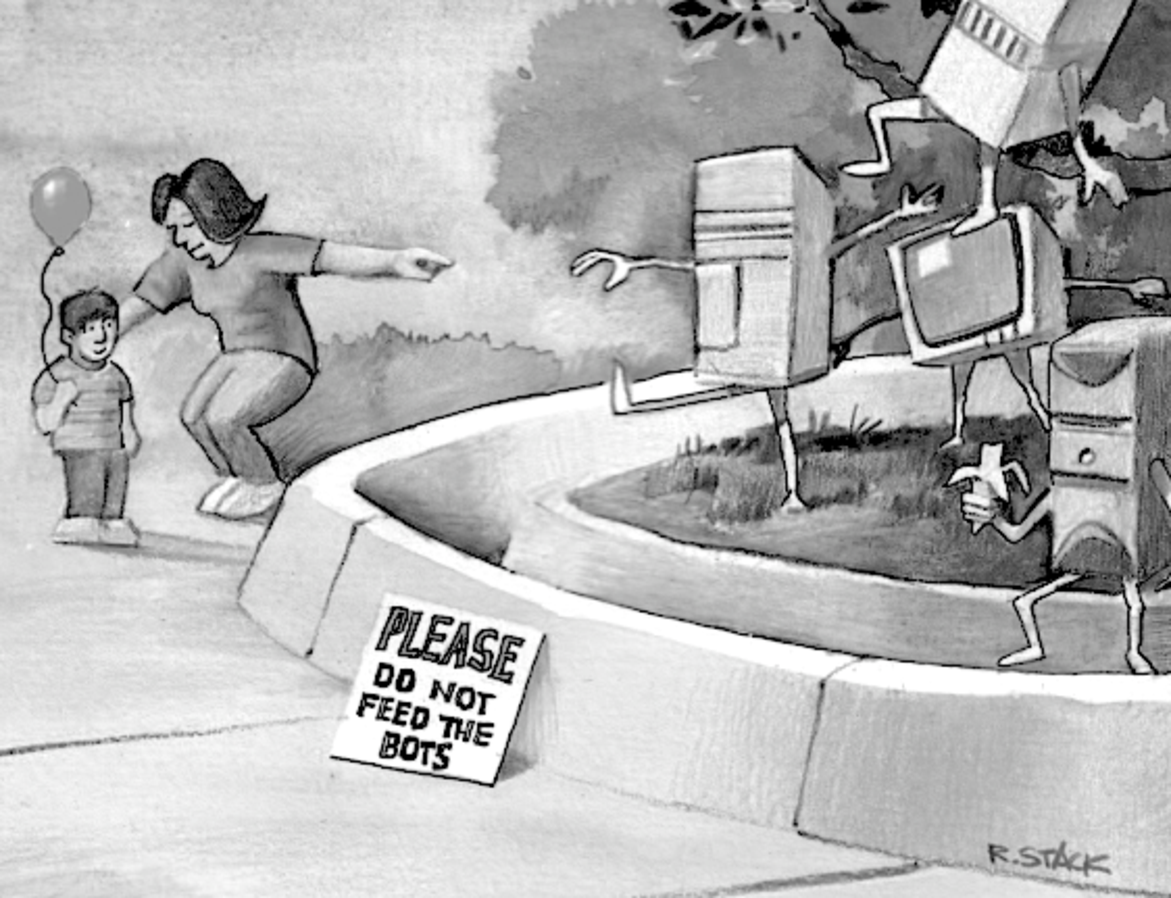
\includegraphics[width=\textwidth]{figures/intro/bots}
  \caption{Illustration taken from~\citep{holz} and \copyright 2005
  IEEE. Authorized license limited to \polimi.}
  \label{fig:bots}
\end{figure}

\begin{quotation}
  [...] the current threat landscape --- such as the increasing
  complexity and sophistication of attacks, the evolution of attackers
  and attack patterns, and malicious activities being pushed to
  emerging countries --- show not just the benefits of, but also the
  need for increased cooperation among security companies,
  governments, academics, and other organizations and individuals to
  combat these changes~\citep{symantec_threat_report_2009}.
\end{quotation}

Todays' underground economy run a very proficient market: everyone can
buy credit card information for as low as \$0.06--\$30, full
identities for just \$0.70--\$60 or rent a scam hosting solution for
\$3--\$40 per week plus \$2-\$20 for the
design~\citep{symantec_threat_report_2009}.

The main underlying technology actually employs a classic type of
software called \emph{bot} (jargon for \emph{robot}), which is not
malicious \emph{per s\'e}, but is used to remotely control a network
of compromised hosts, called \emph{botnet}~\citep{holz}. Remote
commands can be of any type and typically include launching an attack,
starting a phishing or spam campaign, or even updating to the latest
version of the bot software by downloading the binary code from a host
controlled by the attackers (usually called \emph{bot
master})~\citep{torpig}. The exchange good has now become the botnet
infrastructure itself rather than the data that can be stolen or the
spam that can be sent. These are mere outputs of todays' most popular
service offered for rent by the underground economy.

\subsection{The Role of Intrusion Detection}
\label{introduction:motivation:ids-role}
The aforementioned, dramatic big picture may lead to think that the
malicious software will eventually proliferate at every host of the
Internet and no effective remediation exists. However, a more careful
analysis reveals that, despite the complexity of this scenario, the
problems that must be solved by a security infrastructure can be
decomposed into relatively simple tasks that, surprisingly, may
already have a solution. Let us look at an example.

\begin{example}
  This is how a sample exploitation can be structured:
  \begin{description}
  \item [injection] --- a malicious request is sent to the vulnerable
  web application with the goal of corrupting all the responses sent
  to legitimate clients from that moment on. For instance, more than
  one releases of the popular \textsf{WordPress} blog application are
  vulnerable to injection
  attacks\footnote{http://secunia.com/advisories/23595} that allow an
  attacker to permanently include arbitrary content to the
  pages. Typically, such an arbitrary content is malicious code (e.g.,
  JavaScript, VBSCrip, ActionScript, ActiveX) that, every time a
  legitimate user requests the infected page, executes on the client
  host.
  \item [infection] --- Assuming that the compromised site is
  frequently accessed --- this might be the realistic case of the
  \textsf{WordPress}\hyp{}powered \textsf{ZDNet} news
  blog\footnote{http://wordpress.org/showcase/zdnet/} --- a
  significant amount of clients visit it. Due to the high popularity
  of vulnerable browsers and plug-ins, the client may run
  \textsf{Internet Explorer} --- that is the most popular --- or an
  outdated release of \textsf{Firefox} on \textsf{Windows}. This
  create the perfect circumstances for the malicious page to
  successfully execute. In the best case, it may download a virus or a
  generic malware from a website under control of the attacker, so
  infecting the machine. In the worst case, this code may also exploit
  specific browser vulnerabilities and execute in privileged mode.
  \item [control \& use] --- The malicious code just download installs
  and hides itself onto the victim's computer, which has just joined a
  botnet. As part of it, the client host can be remotely controlled by
  the attackers who can, for instance, rent it, use its bandwidth and
  computational power along with other computers to run a distributed
  \ac{DoS} attack. Also, the host can be used to automatically perform
  the same attacks described above against other vulnerable web
  applications. And so forth.
  \end{description}
\end{example}

This simple yet quite realistic example shows the various kinds of
malicious activity that are generated during a typical drive-by
exploitation. It also shows its requirements and assumptions that must
hold to guarantee success. More precisely, we can recognize:

\begin{description}
\item[network activity] --- clearly, the whole interaction relies on a
  network connection over the Internet: the \ac{HTTP} connections
  used, for instance, to download the malicious code as well as to
  launch the injection attack used to compromise the web server.
\item[host activity] --- similarly to every other type of attack
  against an application, when the client-side code executes, the
  browser (or one of its extension plug-ins) is forced to behave
  improperly. If the malicious code executes till completion the
  attack succeeds and the host is infected. This happens only if the
  platform, operating system, and browser all match the requirements
  assumed by the exploit designer. For instance, the attack may
  succeed on \textsf{Windows} and not on \textsf{Mac OS X}, although
  the vulnerable version of, say, \textsf{Firefox} is the same on both
  the hosts.
\item[HTTP traffic] --- in order to exploit the vulnerability of the
  web application, the attacking client must generate malicious
  \ac{HTTP} requests. For instance, in the case of an \ac{SQL}
  injection --- that is the second most common vulnerability in a web
  application --- instead of a regular

  \begin{logs}
    GET /index.php?username=myuser
  \end{logs}
  
\noindent the web server might be forced to process a

\begin{logs}
  GET /index.php?username=' OR 'x'='x'--\&content=<script
  src="evil.com/code.js">
\end{logs}

\noindent that causes the \texttt{index.php} page to behave
improperly.
\end{description}

It is now clear that protection mechanisms that analyze the network
traffic, the activity of the client's operating system, the web
server's \ac{HTTP} logs, or any combination of the three, have chances
of recognizing that something malicious is happening in the
network. For instance, if the \ac{ISP} network adopt \textsf{Snort}, a
lightweight \ac{IDS} that analyzes the network traffic for known
attack patterns, could block all the packets marked as
suspicious. This would prevent, for instance, the \ac{SQL} injection
to reach the web application. A similar protection level can be
achieved by using other tools such as \textsf{ModSecurity}
\citep{ristic:mod_security}. One of the problems that may arise with
these classic, widely adopted solutions is if a zero day\index{0-day}
attack is used. A zero day attack or threat exploits a vulnerability
that is unknown to the public, undisclosed to the software vendor, or
a fix is not available; thus, protection mechanisms that merely
blacklist known malicious activity immediately become ineffective. In
a similar vein, if the client is protected by an anti-virus, the
infection phase can be blocked. However, this countermeasure is once
again successful only if the anti-virus is capable of recognizing the
malicious code, which assumes that the code is known to be malicious.

Ideally, an effective and comprehensive countermeasure can be achieved
if all the protection tools involved (e.g., client\hyp{}side,
server\hyp{}side, network\hyp{}side) can collaborate together. For
instance, if a website is publicly reported to be malicious, a
client\hyp{}side protection tool should block all the content
downloaded from that particular website. This is only a simple
example.

Thus, countermeasures against todays' threats already exist but are
subject to at least two drawbacks:

\begin{itemize}
\item they offer protection only against known threats. To be
effective we must assume that all the hostile traffic can be
enumerated, which is clearly an impossible task.

  \begin{quotation}
    Why is ``Enumerating Badness'' a dumb idea? It's a dumb idea
    because sometime around 1992 the amount of Badness in the Internet
    began to vastly outweigh the amount of Goodness. For every
    harmless, legitimate, application, there are dozens or hundreds of
    pieces of malware, worm tests, exploits, or viral code. Examine a
    typical antivirus package and you'll see it knows about 75,000+
    viruses that might infect your machine. Compare that to the
    legitimate 30 or so apps that I've installed on my machine, and
    you can see it's rather dumb to try to track 75,000 pieces of
    Badness when even a simpleton could track 30 pieces of
    Goodness~\citep{ranum-myths}.
  \end{quotation}

\item they lack of cooperation, which is crucial to detect global and
slow attacks.
\end{itemize}

This said, we conclude that classic approaches such as dynamic and
static code analysis and \ac{IDS} already offer good protection but
industry and research should move toward methods that require little
or no knowledge. In this work, we indeed focus on the so called
anomaly-based approaches, i.e., those that attempt to recognize the
threats by detecting any variation from a system's normal operation,
rather than looking for signs of known\hyp{}to\hyp{}be\hyp{}malicious
activity.

\section{Original Contributions}
\label{introduction:contributions} Our main research area is
\ac{ID}. In particular, we focus on anomaly-based approaches to detect
malicious activities. Since todays' threats are complex, a single
point of inspection is not effective. A more comprehensive monitoring
system is more desirable to protect both the network, the applications
running on a certain host, and the web applications (that are
particularly exposed due to the immense popularity of the Web). Our
contributions focus on the mitigation of both host-based and web-based
attacks, along with two techniques to correlate alerts from hybrid
sensors.

\subsection{Host-based Anomaly Detection} Typical malicious processes
can be detected by modeling the characteristics (e.g., type of
arguments, sequences) of the system calls executed by the kernel, and
by flagging unexpected deviations as attacks. Regarding this type of
approaches, our contributions focus on hybrid models to accurately
characterize the behavior of a binary application. In particular:

\begin{itemize}
\item we enhanced, re-engineered, and evaluated a novel tool for
  modeling the normal activity of the Linux 2.6 kernel. Compared to
  other existing solutions, our system shows better detection
  capabilities and good contextualization of the alerts
  reported. These results are detailed in Section~\ref{host:syscall}.
\item We engineered and evaluated an \ac{IDS} to demonstrate that the
  combined use of (1) deterministic models to characterize a process'
  control flow and (2) stochastic models to capture normal features of
  the data flow, lead to better detection accuracy. Compared to the
  existing deterministic and stochastic approaches separately, our
  system shows better accuracy, with almost zero false
  positives. These results are detailed in
  Section~\ref{host:improving}.
\item We adapted our techniques for forensics investigation. By
  running experiments on real-world data and attacks, we show that our
  system is able to detect hidden tamper evidence although
  sophisticated anti-forensics tools (e.g., userland process
  execution) have been used. These results are detailed in
  Section~\ref{host:forensics}.
\end{itemize}

\subsection{Web-based Anomaly Detection} Attempts of compromising a
web application can be detected by modeling the characteristics (e.g.,
parameter values, character distributions, session content) of the
\ac{HTTP}\index{HTTP} messages exchanged between servers and clients
during normal operation. This approach can detect virtually any
attempt of tampering with \ac{HTTP}\index{HTTP} messages, which is
assumed to be evidence of attack. In this research field, our
contributions focus on training data scarcity issues along with the
problems that arise when an application changes its legit behavior. In
particular:

\begin{itemize}
\item we contributed to the development of a system that learns the
  legit behavior of a web application. Such a behavior is defined by
  means of features extracted from 1) HTTP requests, 2) HTTP
  responses, 3) SQL queries to the underlying database, if any. Each
  feature is extracted and learned by using different models, some of
  which are improvements over well-known approaches and some others
  are original. The main contribution of this work is the
  \emph{combination} of database query models with HTTP-based
  models. The resulting system has been validated through preliminary
  experiments that shown very high accuracy. These results are
  detailed in Section~\ref{web:intro:masibty}.
\item we developed a technique to automatically detect legit changes
  in web applications with the goal of suppressing the large amount of
  false detections due to code upgrades, frequent in todays' web
  applications. We run experiments on real-world data to show that our
  simple but very effective approach accurately predict changes in web
  applications and can distinguish good \emph{vs.} malicious changes
  (i.e., attacks). These results are detailed in
  Section~\ref{web:conceptdrift}.
\item We designed and evaluated a machine learning technique to
  aggregate \ac{IDS} models with the goal of ensuring good detection
  accuracy even in case of scarce training data available. Our
  approach relies on clustering techniques and nearest-neighbor search
  to look-up well-trained models used to replace under-trained ones
  that are prone to overfitting and thus false detections. Experiments
  on real-world data have shown that almost every false alert due to
  overfitting is avoided with as low as 32-64 training samples per
  model. These results are described in Section~\ref{web:longtail}.
\end{itemize}

Although these techniques have been developed on top of a web-based
anomaly detector, they are sufficiently generic to be easily adapted
to other systems using learning approaches.

\subsection{Alert Correlation} \ac{IDS} alerts are usually
post-processed to generate compact reports and eliminate redundant,
meaningless, or false detections. In this research field, our
contributions focus on unsupervised techniques applied to aggregate
and correlate alert events with the goal of reducing the effort of the
security officer. In particular:

\begin{itemize}
\item We developed and tested an approach that accounts for the common
measurement errors (e.g., delays and uncertainties) that occur in the
alert generation process. Our approach exploits fuzzy metrics both to
model errors and to construct an alert aggregation criterion based on
distance in time. This technique has been show to be more robust
compared to classic time-distance based aggregation metrics. These
results are detailed in Section~\ref{correlation:fusion}.
\item We designed and tested a prototype that models the alert
generation process as a stochastic process. This setting allowed us to
construct a simple, non-parametric hypothesis test that can detect
whether two alert streams are correlated or not. Besides its
simplicity, the advantage of our approach is to not requiring any
parameter. These results are described in
Section~\ref{correlation:causality}.
\end{itemize}

The aforementioned results have been published in the proceedings of
international conferences and international journals.

\section{Document Structure}
\label{introduction:structure} This document is structured as
follows. Chapter~\ref{detection} introduces the \ac{ID}, that is the
topic of our research. In particular, Chapter~\ref{detection}
rigorously describes all the basic components that are necessary to
define the \ac{ID} task and an \acp{IDS}. The reader with knowledge on
this subject may skip the first part of the chapter and focus on
Section~\ref{detection:ad} and \ref{detection:correlation} that
include a comprehensive review of the most relevant and influential
modern approaches on network-, host-, web-based \ac{ID} techniques,
along with a separate overview of the alert correlation approaches.

As described in Section~\ref{introduction:contributions}, the
description of our contributions is structured into three
chapters. Chapter~\ref{host} focuses on host-based techniques,
Chapter~\ref{web} regards web-based anomaly detection, while
Chapter~\ref{correlation} described two techniques that allow to
recognize relations between alerts reported by network- and host-based
systems. Reading Section~\ref{detection:ad:network} is recommended
before reading Chapter~\ref{correlation}.

The reader interested in protection techniques for the operating
system can skim through Section~\ref{detection:ad:host} and then read
Chapter~\ref{host}. The reader with interests on web-based protection
techniques can read Section~\ref{detection:ad:web} and then
Chapter~\ref{web}. Similarly, the reader interested in alert
correlation systems can skim through
Section~\ref{detection:ad:network} and \ref{detection:ad:host} and
then read Chapter~\ref{correlation}.

%%% Local Variables: 
%%% mode: latex
%%% TeX-master: "thesis"
%%% End: 


\let\stdsection\section
\renewcommand\section{\newpage\stdsection}

\chapter{Detecting Malicious Activity}
\label{detection}
Malicious activity is a generic term that refers to automated or
manual attempts of compromising the security of a computer
infrastructure. Examples of malicious activity include the output
generated (or its effect on a system) by the execution of simple
script kiddies, viruses, \ac{DoS} attacks, exploits of \ac{XSS} or
\ac{SQL} injection vulnerabilities, and so forth. This chapter
describes the research tools and methodologies available to detect and
mitigate malicious activity on a network, a single host, a web-server
and the combination of the three.

First, the background concepts and the \ac{ID} problem are described
in this chapter along with a taxonomic description of the most
relevant aspects of an \ac{IDS}. Secondly, a detailed survey of the
selected state-of-the-art anomaly detection approaches is presented
with the help of further classification dimensions. In addition, the
problem of alert correlation, that is an orthogonal topic, is
described and the most relevant, recent research approaches are
overviewed. Last but not least, the problem of evaluating an \ac{IDS}
is presented to provide the essential terminology and criteria to
understand the effectiveness of both the reviewed literature and our
original contributions.

\section{Intrusion Detection}
\label{detection:id}
\ac{ID} is the practice of analyzing a system to find malicious
activity. This section defines this concept more precisely by means of
simple but rigorous definitions. The context of such definitions is
the generic scenario of an Internet site, for instance, the network of
an \ac{ISP}. An example is depicted in
Figure~\ref{fig:ids-generic-scenario}. An Internet site ---and, in
general, the Internet itself--- is the state-of-the-art computer
infrastructure. In fact, it is a network that adopts almost any kind
of known computer technology (e.g., protocols, standards, containment
measures), it runs a rich variety of servers such as
\ac{HTTP}\index{HTTP}, \ac{FTP}\index{FTP}, \ac{SSH}\index{SSH},
\ac{VPN}\index{VPN} to support a broad spectrum of sophisticated
applications and services (e.g., web applications, e-commerce,
applications, the \textsf{Facebook Platform}, \textsf{Google
  Applications}). In addition, a generic Internet site receives and
process traffic from virtually any user connected to the Net and thus
represents the perfect research testbed for \ac{IDS}.

\begin{figure}[t]
  \centering
  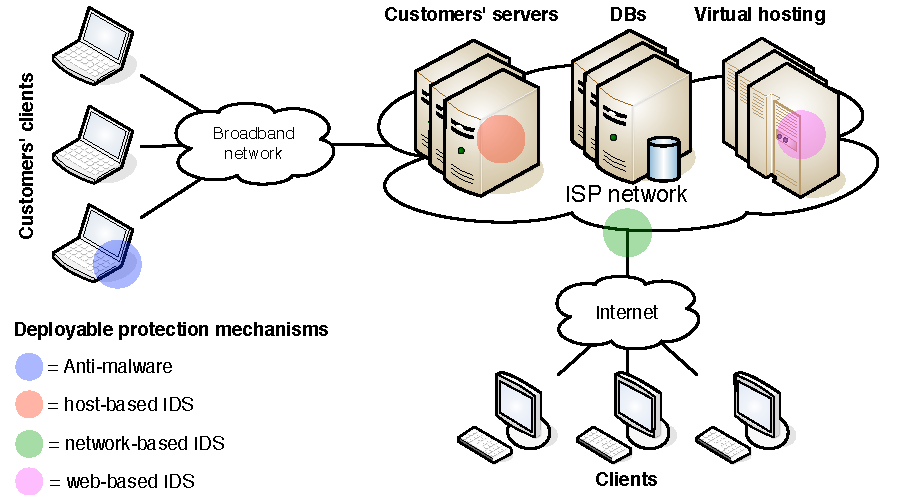
\includegraphics[width=\textwidth]{figures/detection/ids-generic-scenario}
  \caption{Generic and comprehensive deployment scenario for
  \acp{IDS}\index{IDS}.}
  \label{fig:ids-generic-scenario}
\end{figure}

\begin{definition}[System]
  A \emph{system} is the domain of interest for security.
\end{definition}

\noindent Note that a system can be a physical or a logical one. For
instance, a physical system could be a host (e.g., the
\ac{DB}\index{DB} server or one of the client machines shown in the
figure), a whole network (e.g., the \ac{ISP} network shown in the
figure); a logical system can be an application, a service, such as
one of the web services run in a virtual machine deployed in the
\ac{ISP} network. While running, each system produces \emph{activity},
that we define as follows.

\begin{definition}[System activity]
  A system \emph{activity} is any data generated while the system is
  working. Such activity is formalized a sequence of events
  $\mathbb{I} = [I_{1}, I_{2}, I_{i}, \dots, I_{N}]$.
\end{definition}

\noindent For instance, each of the clients of
Figure~\ref{fig:ids-generic-scenario} produces system logs: in this
case $\mathbb{I}$ would contain an $I_{i}$ for each log entry. A human
readable representation follows.

\begin{logs} Aug 18 00:30:22 Adium[55011]: Warning: -[AIChatController
chatWithContact:(null)] got a nil targetContact.  Aug 18 00:29:40
[0x0-0x1b01b].org.mozilla.firefox[0]: NPP_Initialize called Aug 18
00:29:40 [0x0-0x1b01b].org.mozilla.firefox[0]: 2009-08-18 00:29:40.039
firefox-bin[254:10b] NPP_New(instance=0x169e0178,mode=2,argc=5) Aug 18
00:29:40 [0x0-0x1b01b].org.mozilla.firefox[0]: 2009-08-18 00:29:40.052
firefox-bin[254:10b] NPP_NewStream end=396239
\end{logs}

Similarly, the web servers generates \ac{HTTP}\index{HTTP} requests
and responses: in this case $\mathbb{I}$ would contain an $I_{i}$ for
each \ac{HTTP}\index{HTTP} message. Its human readable representation
follows.

\begin{logs} 128.111.48.4 [20/May/2009:15:25:42 -0700] "GET
/media//images/favicon.ico HTTP/1.0" 200 1150 "-" "Mozilla/5.0
(Macintosh; U; Intel Mac OS X 10.5; en-US; rv:1.9.0.10)
Gecko/2009042315 Firefox/3.0.10 Ubiquity/0.1.4" 128.111.48.4
[20/May/2009:15:26:44 -0700] "POST /report/ HTTP/1.0" 200 19171
"http://www.phonephishing.info/report/" "Mozilla/5.0 (Macintosh; U;
Intel Mac OS X 10.5; en-US; rv:1.9.0.10) Gecko/2009042315
Firefox/3.0.10 Ubiquity/0.1.4" 128.111.48.4 [20/May/2009:15:26:44
-0700] "GET /media//css/main.css HTTP/1.0" 200 5525
"http://www.phonephishing.info/report/" "Mozilla/5.0 (Macintosh; U;
Intel Mac OS X 10.5; en-US; rv:1.9.0.10) Gecko/2009042315
Firefox/3.0.10 Ubiquity/0.1.4" 128.111.48.4 [20/May/2009:15:26:44
-0700] "GET /media//css/roundbox.css HTTP/1.0" 200 731
"http://www.phonephishing.info/media//css/main.css" "Mozilla/5.0
(Macintosh; U; Intel Mac OS X 10.5; en-US; rv:1.9.0.10)
Gecko/2009042315 Firefox/3.0.10 Ubiquity/0.1.4"
\end{logs}

Other examples of system activity are described in Section
\ref{detection:id:taxonomy}.

In this document, we often used the term \emph{normal behavior}
referring to a set of characteristics (e.g., the distribution of the
characters of string parameters, the mean and standard deviation of
the values of integer parameters) extracted from the system activity
gathered during normal operation (i.e., without being
compromised). Moreover, in the remainder of this document, we need
other definitions.

\begin{definition}[Activity Profile]\label{def:activity-model}
  The \emph{activity profile} (or activity model) $c_{\mathbb{I}}$ is
  a set of models
  \begin{displaymath}
    c_{\mathbb{I}} = \langle m^{(1)}, \dots, m^{(u)}, \dots, m^{(U)}
    \rangle
  \end{displaymath} generated by extracting features from the system
  activity $\mathbb{I}$.
\end{definition}

\noindent This definition will be used in
Section~\ref{sec:misuse-vs-anomaly} and
Example~\ref{ex:misuse-vs-anomaly} and
\ref{ex:character-distribution-model} describe an instance of
$m^{(u)}$. An example of a real-world profile is described in
Example~\ref{ex:web-models}. We can now define the:

\begin{definition}[System Behavior]\label{def:system-behavior}
  The \emph{system behavior} is the set of features (or models), along
  with their numeric values, extracted by (or contained in) the
  activity profile.
\end{definition}

In particular, we will use this term as a synonym of \emph{normal}
system behavior, referring to the system behavior during normal
operation.

Given the high-accessibility of the Internet, publicly available
systems such as web servers, web applications, \ac{DB}\index{DB}
servers, are constantly at risk. In particular, they can be
compromised with the goal of stealing valuable information, deploying
infection kits or running phishing\index{phishing} and spam
campaigns. These are all examples of \emph{intrusions}. More formally.

\begin{definition}[Intrusion]
  An \emph{intrusion} is the automated or manual act of violating one
  or more security paradigms (i.e., confidentiality, integrity,
  availability) of a system. Intrusions are formalized as a sequence
  of events:

  \begin{displaymath}
    \mathbb{O} = [O_{1}, O_{2}, O_{i}, \dots, O_{M}] \subseteq
    \mathbb{I}
  \end{displaymath}
\end{definition}

\noindent Typically, when an intrusion takes place, a system behaves
unexpectedly and, as a consequence, its activity differs than during
normal operation. This is because an attack or the execution of
malware\index{malware} code often exploit vulnerabilities to bring the system into
states it was not designed for. For this reason, the activity that the
system generates is called \emph{malicious activity}; often, this term
is also used to indicate the attack or the malware\index{malware} code execution
itself. An example of $O_{i}$ is the following log entry: it shows
evidence of a \ac{XSS} attack that will make a vulnerable page to
display the arbitrary content supplied as part of the GET request
(while the page was not intentionally designed to this purpose).

\begin{logs} 128.111.48.4 [20/May/2009:15:29:44 -0700] "GET
/report/add/comment/<DIV
STYLE="background-image:\0075\0072\006C\0028'\006a\0061\0076\0061\0073\0063\0072\0069\0070\0074\003a\0061\006c\0065\0072\0074\0028.1027\0058.1053\0053\0027\0029'\0029">/
HTTP/1.0" 200 731 "http://www.phonephishing.info/report/add/"
"Mozilla/5.0 (Macintosh; U; Intel Mac OS X 10.5; en-US; rv:1.9.0.10)
Gecko/2009042315 Firefox/3.0.10 Ubiquity/0.1.4"
\end{logs}

\begin{note}
  We adopt a simplified representation of intrusions with respect to a
  dataset $\mathbb{D}$ (i.e., both normal and malicious): with
  $\mathbb{O} \subseteq \mathbb{D}$ we indicate that the activity
  $\mathbb{I}$ contains malicious events $\mathbb{O}$; however,
  strictly speaking, intrusions events and activity events can be of
  completely different types, thus the ''$\subseteq$'' relation may
  not be defined in a strict mathematical sense.
\end{note}

\noindent If a system is well-designed, any intrusion attempts always
leave some traces in the system's activity. These traces are called
\emph{tamper evidence} and are essential to perform \emph{intrusion
detection}.

\begin{definition}[Intrusion Detection]
  Intrusion \emph{detection} is the separation of intrusions from
  normal activity through the analysis of the activity of a system,
  while the system is running. Intrusions are marked as \emph{alerts},
  which are formalized as a sequence of event $\mathbb{A} = [A_{1},
  A_{2}, A_{i}, \dots, A_{L}] \subseteq \mathbb{O}$.
\end{definition}

\noindent Similarly, $\mathbb{A} \subseteq \mathbb{O}$ must not be
interpreted in a strict sense: it is just a notation to indicate that
for each intrusion, an alert may or may not exist. Note that \ac{ID}
can be also performed by manually inspecting a system activity. This
is clearly a tedious and unefficient task, thus research and
industrial interests are focused on automatic approaches.

\begin{definition}[Intrusion Detection System]
  An \emph{intrusion detection system} is an automatic tool that
  performs the \ac{ID} task.
\end{definition}

\noindent Given the above definitions, an abstract model of an
\ac{IDS} is shown in Figure~\ref{fig:ids-abstract-model}.

\begin{figure}[t]
  \centering
  \begin{tikzpicture}[node distance=6em]
    \node (I) {$\mathbb{I}, \mathbb{O}$}; \node
    [draw,shape=rectangle,inner sep=1em] (ids) [right of=I] {IDS};
    \node (A) [right of=ids] {$\mathbb{A}$}; \draw[-stealth] (I) --
    (ids); \draw[-stealth] (ids) -- (A);
  \end{tikzpicture}
  \caption{Abstract I/O model of an \ac{IDS}.}
  \label{fig:ids-abstract-model}
\end{figure}

Although each \ac{IDS} relies on its own data model and format to
represent $\mathbb{A}$, the \ac{IETF} proposed \ac{IDMEF}
\citep{IDMEF} as a common format for reporting alert streams generated
by different \ac{IDS}.

\subsection{Evaluation}
\label{detection:evaluation} Evaluating an \ac{IDS} means running it
on collected data $\mathbb{D} = \mathbb{I} \cup \mathbb{O}$ that
resembles real-world scenarios. This means that such data includes
both intrusions $\mathbb{O}$ and normal activity $\mathbb{I}$, i.e.,
$|\mathbb{I}|, |\mathbb{O}| > 0$ and $\mathbb{I} \cap \mathbb{O} =
\varnothing$, i.e., $\mathbb{I}$ must include no malicious activity
other than $\mathbb{O}$.  The system is run in a controlled
environment to collect $\mathbb{A}$ along with performance indicators
for comparison with other systems. This section presents the basic
criteria used to evaluate modern \acp{IDS}\index{IDS}.

More precisely, to perform an evaluation experiment correctly a
fundamental hypothesis must hold: the set $\mathbb{O}$ must be known
and perfectly distinguishable from $\mathbb{I}$. In other words, this
means that, $\mathbb{D}$ must be labeled with a \emph{truth file},
i.e., a list of all the events known to be malicious. This allows to
treat the \ac{ID} problem as a classic classification problem, for
which a set of well-established evaluation metrics are available. In
particular, we are interested at calculating the following sets.

\begin{definition}[\acfp{TP}\index{TP}]
  The set of \emph{true positives} is $TP := \{A_{i} \in \mathbb{A}
  \mid \exists O_{j}: f(A_{i}) = O_{j}\}$.
\end{definition}

\noindent Where $f: \mathbb{A} \mapsto \mathbb{O}$ is a generic
function that, given an alert $A_{i}$ finds the corresponding
intrusion $O_{j}$ by parsing the truth file. The $TP$ set is basically
the set of alerts that are fired because a real intrusion has taken
place. The perfect \ac{IDS} is such that $TP \equiv \mathbb{O}$.

\begin{definition}[\acfp{TP}\index{TP}]
  The set of \emph{false positives} is
  \begin{displaymath}
    FP := \{A_{i} \in \mathbb{A} \mid \not\exists O_{j}: f(A_{i}) =
    O_{j}\}.
  \end{displaymath}
\end{definition}

\noindent On the other hand, the alerts in $FP$ are incorrect because
no real intrusion can be found in the observed activity. The perfect
\ac{IDS} is such that $FP = \varnothing$.

\begin{definition}[\acfp{TN}\index{TN}]
  The set of \emph{true negatives} is
  \begin{displaymath}
    TN := \{I_{j} \in \mathbb{I} \mid \not\exists A_{i}: f(A_{i}) =
    I_{j}\}.
  \end{displaymath}
\end{definition}

\noindent Note that the set of $TN$ does not contain
alerts. Basically, it is the set of correctly unreported alerts. The
perfect \ac{IDS} is such that $TN \equiv \mathbb{I}$.

\begin{definition}[\acfp{FN}\index{FN}]
  The set of \emph{false negatives} is
  \begin{displaymath}
    FN := \{O_{j} \in \mathbb{O} \mid \not\exists A_{i}: f(A_{i}) =
    O_{j}\}.
  \end{displaymath}
\end{definition}

\noindent Similarly to $TN$, $FN$ does not contain alerts. Basically,
it is the set of incorrectly unreported alerts. The perfect \ac{IDS}
is such that $FN = \varnothing$. Note that, $TP + TN + FP + TN = 1$
must hold.

In this and other documents, the term \emph{false alert} refers to $FN
\cup FP$. Given the aforementioned sets, aggregated measures can be
calculated.

\begin{definition}[\ac{DR}]
  The \emph{detection rate}, or \emph{true positive rate}, is defined
  as:

  \begin{displaymath}
    DR := \frac{TP}{TP + FN}.
  \end{displaymath}
\end{definition}

\noindent The perfect \ac{IDS} is such that $DR = 1$. Thus, the
\ac{DR} measures the detection capabilities of the system, that is,
the amount of malicious events correctly classified and reported as
alerts. On the other side, the \ac{FPR} is defined as follows.

\begin{definition}[\ac{FPR}]
  The \emph{false positive rate} is defined as:

  \begin{displaymath}
    FPR := \frac{FP}{FP + TN}.
  \end{displaymath}
\end{definition}

\noindent The perfect \ac{IDS} is such that $FPR = 0$. Thus, the
\ac{FPR} measures the inaccuracies of the system, that is, the amount
of legit events incorrectly classified and reported as alerts. There
are also other metrics such as the \emph{accuracy} and the
\emph{precision} which are often used to evaluate information
retrieval systems; however, these metrics are not popular for \ac{IDS}
evaluation.

\begin{figure}[tt]
  \centering
  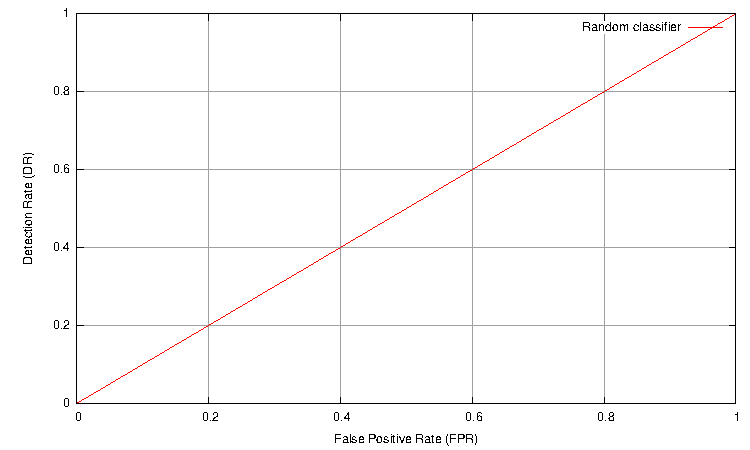
\includegraphics[width=.8\textwidth]{figures/detection/roc-space}
  \caption{The \ac{ROC} space.}
  \label{fig:roc-space}
\end{figure}

The \ac{ROC} analysis, originally adopted to measure transmission
quality of radar systems, is often used to produce a compact and easy
to understand evaluation of classification systems. Even though there
is no standardized procedure to evaluate an \ac{IDS}, the research
community agrees on the use of \ac{ROC} curves to compare the
detection capabilities and quality of an \ac{IDS}. A \ac{ROC} curve is
the plot of $DR = DR(FPR)$ and is obtained by tuning the \ac{IDS} to
trade off \acp{FP}\index{FP} against true positives. Without going
into the details, each point of a \ac{ROC} curve correspond to a fixed
amount of $DR$ and $FPR$ calculated under certain conditions (e.g.,
sensitivity parameters). By modifying its configuration the quality of
the classification changes and other points of the \ac{ROC} are
determined. The \ac{ROC} space is plotted in
Figure~\ref{fig:roc-space} along with the performances of a random
classifiers, characterized by $DR = FPR$. The perfect, ideal \ac{IDS}
can increase its $DR$ from 0 to 1 with $FPR = 0$: however, it must
hold that $FPR \to 1 \Rightarrow DR \to 1$.

\subsection{Alert Correlation}
\label{detection:id:alert-correlation} The problem of intrusion
detection is challenging in todays' complex networks. In fact, it is
common to have more than one \ac{IDS}\index{IDS} deployed, monitoring
different segments and different aspects of the whole infrastructure
(e.g., hosts, applications, network, etc.). The amount of alerts
reported by a network of \acp{IDS}\index{IDS} running in a complex
computer infrastructure is larger, by several orders of magnitude,
than what was common in the smaller networks monitored years ago. In
such a context, network administrators are loaded by several alerts
and long security reports often containing a non-negligible amount of
\acp{FP}\index{FP}. Thus, the creation of a clean, compact, and
unified view of the security status of the network is needed. This
process is commonly known as alert correlation
\citep{valeur04comprehensive} and it is currently one of the most
difficult challenges of this research field. More precisely.

\begin{definition}[Alert Correlation]
  The \emph{alert correlation} is the identification of relations
  among alerts

  \begin{displaymath}
    A_{1}, A_{2}, A_{i}, \dots, A_{L} \in \mathbb{A}_{1} \cup
    \mathbb{A}_{2} \cup \cdots \cup \mathbb{A}_{K}
  \end{displaymath}

  to generate a unique, more compact and comprehensive sequence of
  alerts $\mathbb{A'} = [A'_{1}, A'_{2}, \dots, A'_{P}]$.
\end{definition}

A desirable property is that $\mathbb{A}'$ should be as complete as
$\mathbb{A}_{1} \cup \mathbb{A}_{2} \cup \cdots \cup \mathbb{A}_{K}$
without introducing errors such as alerts that do not correspond to a
real intrusion. As for the \ac{ID}, alert correlation can be a manual,
and tedious, task. Clearly, automatic alert correlation systems are
more attractive and can be considered a complement of a modern
\ac{IDS}.

\begin{definition}[Alert Correlation System]
  An \emph{alert correlation system} is an automatic tool that
  performs the alert correlation task.
\end{definition}

\noindent The overall \ac{IDS} abstract model is complemented with an
alert correlation engine as shown in
Figure~\ref{fig:ids-ac-abstract-model}.

\begin{figure}[t]
  \centering
  \begin{tikzpicture}[node distance=6em]
    \node (I) {$\mathbb{I}, \mathbb{O}$}; \node
    [draw,shape=rectangle,inner sep=1em,double copy shadow,fill=white]
    (ids) [right of=I] {IDS}; \node (A) [right of=ids,text
    width=1.2em] {$\mathbb{A}_{1}$\\...\\$\mathbb{A}_{n}$}; \node
    [draw,shape=rectangle,inner sep=1em,fill=white] (acs) [right of=A]
    {ACS}; \node (Ap) [right of=acs] {$\mathbb{A}'$}; \draw[-stealth]
    (I) -- (ids); \draw[-stealth] (ids) -- (A); \draw[-stealth] (A) --
    (acs); \draw[-stealth] (acs) -- (Ap);
  \end{tikzpicture}
  \caption{Abstract I/O model of an \ac{IDS} with an alert correlation
  system.}
  \label{fig:ids-ac-abstract-model}
\end{figure}

\subsection{Taxonomic Dimensions}
\label{detection:id:taxonomy}
The first comprehensive taxonomy of \acp{IDS}\index{IDS} has been
proposed in \citep{debar1999towards} and revised in
\citep{debar2000revised}. Another good survey appeared in
\citep{axelsson-intrusion}.

Compared to the classic survey found in the literature, this section
complements the basic taxonomic dimensions by focusing on
\emph{modern} techniques. In particular, todays' intrusion detection
approaches can be categorized by means of the specific modeling
techniques appeared in recent research.

It is important to note that the taxonomic dimensions that are
hereby suggested are not exhaustive, thus certain \acp{IDS} may not
fit into it (e.g.,
\citep{vigilante,argos:eurosys06,newsome2005dynamic}). On the other
hand, an exhaustive and detailed taxonomy would be difficult to
read. To overcome this difficulty, in this section we describe a
high-level, technique-agnostic taxonomy based on the dimensions
summarized in Table~\ref{tab:misuse-vs-anomaly}; in each sub-section
of Section~\ref{detection:ad}, which focus on anomaly-based models, we
expand the taxonomic dimensions by listing and accurately detailing
further classification criteria.

\subsubsection{Type of model}
\label{sec:misuse-vs-anomaly} \acp{IDS}\index{IDS} must be divided
into two opposite groups: misuse\hyp{}based \emph{vs.}
anomaly\hyp{}based. The former create models of the \emph{malicious}
activity while the latter create models of \emph{normal}
activity. Misuse-based models look for \emph{patterns} of malicious
activity; anomaly-based models look for \emph{unexpected} activity. In
some sense, \acp{IDS}\index{IDS} can either ``blacklist'' or
``whitelist'' the observed activity.

Typically, the first type of models consists in a database of all the
known attacks. Besides requiring frequent updates ---which is just a
technical difficulty and can be easily automated--- misuse-based
systems assumes the feasibility of enumerating \emph{all} the
malicious activity.

Despite the limitation of being inherently incomplete, misuse-based
systems widely adopted in the real-world
\citep{snortlisa,snortsite}. This is mainly due to their simplicity
(i.e., attack models are triggered by means of pattern matching
algorithms) and accuracy (i.e., they generate virtually no false
alerts because an attack signature can either match or not).

Anomaly-based approaches are more complex because creating a
specification of normal activity is obviously a difficult task. For
this reason, there are no well-established and widely-adopted
techniques; instead, misuse models are as sophisticated as a pattern
matching problem. In fact, the research on anomaly-based systems is
very active.

These systems are effective only under the assumption that malicious
activity, such as an attack or malware\index{malware} being executed, \emph{always}
produces sufficient deviations from normal activity such that models
are triggered, i.e., anomalies. This clearly has the positive
side-effect of requiring zero knowledge on the malicious activity,
which makes these systems particularly interesting. The negative
side-effect is their tendency of producing a significant amount of
false alerts (the notion of ``significant amount of false alerts''
will be discussed in detail in Section
\ref{detection:evaluation:base-rate-fallacy}).

Obviously, an \ac{IDS} can benefit of both the techniques by, for
instance, enumerating all the known attacks and using anomaly-based
heuristics to prompt for suspicious activity. This practice is often
adopted by modern anti-viruses.

It is important to remark that, differently from the other taxonomic
dimensions, the distinction between misuse- and anomaly-based
approaches is fundamental: they are based on opposite hypotheses and
yield to completely different system designs and results. Their
duality is highlighted in Table \ref{tab:misuse-vs-anomaly}.

\begin{table}[t]
  \centering
  \begin{tabular}{rcc}
    \toprule \emph{Feature} & \textsc{Misuse-based} &
    \textsc{Anomaly-based}\\
    
    \midrule Modeled activity: & Malicious &
    Normal\\
    
    Detection method: & Matching & Deviation\\

    Threats
    detected: & Known & Any\\

    False negatives: & High & Low\\

    False
    positives: & Low & High\\

    Maintenance cost: & High & Low\\ Attack
    desc.: & Accurate & Absent\\

    System design: & Easy & Difficult\\
    \bottomrule
  \end{tabular}
  \caption{Duality between misuse- and anomaly-based intrusion
    detection techniques. Note that, an anomaly-based \ac{IDS} can
    detect ``Any'' threat, under the assumption that an attack always
    generates a deviation in the modeled activity.}
  \label{tab:misuse-vs-anomaly}
\end{table}

\begin{example}[Misuse \emph{vs.} Anomaly]\label{ex:misuse-vs-anomaly}
  A misuse-based system $M$ and an anomaly-based system $A$ process
  the same log containing a full dump of the system calls invoked by
  the kernel of an audited machine. Log entries are in the form:

  \begin{center}\small
    \begin{verbatim} <function_name>(<arg1_value>, <arg2_value>, ...)
    \end{verbatim}
  \end{center}

\noindent The system $M$ has the following simple attack
model\footnote{Generated from the real world exploit
\url{http://milw0rm.com/exploits/9303}}:

\begin{pseudoc}
  if (function_name == "read") {
    /* ... */ if (match(decode(arg3_value), "a{4}b{4}c{4}d{4}e{4}\
        f{4}...x{4}3RH~TY7{33}QZjAXP0A0AkAAQ2AB2BB0BBAB\
        XP8ABuJIXkweaHrJwpf02pQzePMhyzWwSuQnioXPOHuBxKn\
        aQlkOjpJHIvKOYokObPPwRN1uqt5PA..." ))
    fire_alert("VLC bug 35500 is being exploited!"); /* ... */
  }
\end{pseudoc}
\end{example}

The simple attack signature looks for a pattern generated from the
exploit. If the content of the buffer (i.e., \texttt{arg3\_value})
that stores the malicious file matches the given pattern then an alert
is fired.

\noindent On the other hand, the system $A$ has the following model,
based on the sample character distribution of each file's
content. Such frequencies are calculated during normal operation of
the application.

\begin{pseudoc}
  /* ... */ cd['<'] = {0.1, 0.11} cd['a'] = {0.01, 0.2} cd['b'] =
  {0.13, 0.23} /* ... */

  b = decode(arg3_value);
  
  if ( !(cd['c'][0] < count('c', b) < cd['c'][1]) ||\
       !(cd['<'][0] < count('<', b) < cd['<'][1]) ||\
       ... || ...)  fire_alert("Anomalous content detected!");
  /* ... */
\end{pseudoc}

Obviously, more sophisticated models can be designed. The purpose of
this example is that of highlighting the main differences between the
two approaches.

\medskip

A generalization of the aforementioned examples allows us to better
define an anomaly-based \ac{IDS}.

\begin{definition}[Anomaly-based \ac{IDS}]
  An \emph{anomaly-based \ac{IDS}} is a type of \ac{IDS} that generate
  alerts $\mathbb{A}$ by relying on normal activity profiles
  (Definition~\ref{def:activity-model}).
\end{definition}

\subsubsection{System activity} \acp{IDS}\index{IDS} can be classified
based on the type of the activity they monitor. The classic literature
distinguishes between network\hyp{}based and host\hyp{}based systems;
\ac{NIDS} and \ac{HIDS}, respectively. The former inspect network
traffic (i.e., raw bytes sniffed from the network adapters), and the
latter inspect the activity of the operating system. The scope of a
network-based system is as large as the broadcast domain of the
monitored network. On the other hand, the scope host-based systems is
limited to the single host.

Network-based \acp{IDS}\index{IDS} have the advantage of having a
large scope, while host-based ones have the advantage of being fed
with detailed information about the host they run on (e.g., process
information, \ac{CPU}\index{CPU} load, number of active processes,
number of users). This information is often unavailable to
network-based systems and can be useful to refine a decision regarding
suspicious activity. For example, by inspecting both the network
traffic and the kernel activity, an \ac{IDS} can filter the alerts
regarding the \textsf{Apache} web server version 2.0.0 on all the
hosts running version 2.0.2. On the other hand, network-based systems
are centralized and are much more easy to manage and deploy. However,
\ac{NIDS} are limited to the inspection of unencrypted payload, while
\ac{HIDS} may have it decrypted by the application layer. For example,
a \ac{NIDS} cannot detect malicious HTTPS traffic.

The network stack is standardized (see
Note~\ref{note:network-stack-standardized}), thus the definition of
network-based \ac{IDS} is precise. On the other hand, because of the
immense variety of operating system implementations, a clear
definition of ``host data'' lacks. Existing host-based
\acp{IDS}\index{IDS} analyze audit log files in several formats, other
systems keep track of the commands issued by the users through the
console. Some efforts have been made to propose standard formats for
host data: \ac{BSM}\index{BSM} and its modern re-implementation called
\textsf{OpenBSM} \citep{openbsm,openbsm_site} are probably the most
used by the research community as they allow developers to gather the
full dump of the system calls before execution in the kernel.

\begin{note}\label{note:network-stack-standardized}
  Although the network stack implementation may vary from system to
  system (e.g., \textsf{Windows} and \textsf{Cisco} platforms have
  different implementation of \ac{TCP}), it is important to underline
  that the notion of IP, TCP, HTTP \emph{packet} is well defined in a
  system-agnostic way, while the notion of \emph{operating system
    activity} is rather vague and by no means standardized.
\end{note}

Example \ref{ex:misuse-vs-anomaly} describes a sample host-based
misuse detection system that inspects the arguments of the system
calls. A similar, but more sophisticated, example based on network
traffic is \textsf{Snort} \citep{snortlisa,snortsite}.

\begin{note}[Inspection layer]
  Network-based systems can be further categorized by their protocol
  inspection capabilities, with respect to the network
  stack. \webanomaly \citep{kruegel:jcn2005:webanomaly,webanomalysite}
  is network\hyp{}based, in the sense that runs in promiscuous mode
  and inspects network data. On the other hand, it also
  \ac{HTTP}\index{HTTP}-based, in the sense that decodes the payload
  and reconstructs the \ac{HTTP}\index{HTTP} messages (i.e., request
  and response) to detect attacks against web applications.
\end{note}

\subsubsection{Model construction method} Regardless of their type,
misuse- or anomaly-based, models can be specified either manually or
automatically. However, for their nature, misuse models are often
manually written because they are based on the exhaustive enumeration
of known malicious activity. Typically, these models are called attack
signatures; the largest repository of manually generated misuse
signatures is released by the \textsf{Sourcefire Vulnerability
Research Team\texttrademark} \citep{snortrules}. Misuse signatures can
be generated automatically: for instance, in \citep{1251258} a method
to build misuse models of worms is described. Similarly,
low-interaction honeypots often uses malware\index{malware} emulation to
automatically generate signatures. Two recently proposed techniques
are \citep{argos:eurosys06,1224380}.

On the other hand, anomaly-based models are more suitable for
automatic generation. Most of the anomaly-based approaches in the
literature focus on unsupervised learning mechanisms to construct
models that precisely capture the normal activity observed. Manually
specified models are typically more accurate and are less prone to
\acp{FP}\index{FP}, although automatic techniques are clearly more
desirable.

\begin{example}[Learning character
distributions]\label{ex:character-distribution-model}
  In Example \ref{ex:misuse-vs-anomaly}, the described system $A$
  adopts a learning based character distribution model for
  strings. Without going into the details, the idea described in
  \citep{mutz06:syscalls} observes string arguments and estimate the
  characters' distribution over the \ac{ASCII}\index{ASCII} set. More
  practically, the model is a histogram $H(c), \forall c \in {0,
  255}$, where $H(c)$ is the normalized frequency of character
  $c$. During detection, a $\chi^{2}$ test is used to decide whether
  or not a certain sting is deemed anomalous.

Beside the obvious advantage of being resilient against evasion, this
model requires no human intervention.
\end{example}

\section{Relevant Anomaly Detection Techniques}
\label{detection:ad} Our research focuses on anomaly detection. In
this section, the selected state of the art approaches are reviewed
with particular attention to network\hyp{}, host\hyp{} and
web\hyp{}based techniques, along with the most influential approaches
in the recent literature alert correlation. This section provides the
reader with the basic concepts to understand our contributions.

\subsection{Network-based techniques}
\label{detection:ad:network}
Our research does not include network-based \acp{IDS}\index{IDS}. Our
contributions in alert correlation, however, leverage both network-
and host-based techniques, thus a brief overview of the latest (i.e.,
proposed between 2001 and 2006) network-based detection approaches is
provided in this section. We remark that all the techniques included
in the following are based on \ac{TCP}\index{TCP}/IP, meaning that
models of normal activity are constructed by inspecting the decoded
network frames up to the \ac{TCP}\index{TCP} layer.

In Table \ref{tab:network-sota-taxonomy} the selected approaches are
marked with bullets to highlight their specific characteristics. Such
characteristics are based on our analysis and experience, thus, other
classifications may be possible. They are defined as follows:

\begin{description}
\item[Time] refers to the use of \emph{timestamp} information,
extracted from network packets, to model normal packets. For example,
normal packets may be modeled by their minimum and maximum
inter-arrival time.
\item[Header] means that the \ac{TCP}\index{TCP} header is decoded and
the fields are modeled. For example, normal packets may be modeled by
the observed ports range.
\item[Payload] refers to the use of the payload, either at
\ac{IP}\index{IP} or \ac{TCP}\index{TCP} layer. For example, normal
packets may be modeled by the most frequent byte in the observed
payloads.
\item[Stochastic] means that stochastic techniques are exploited to
create models. For example, the model of normal packets may be
constructed by estimating the sample mean and variance of certain
features (e.g., port number, content length).
\item[Deterministic] means that certain features are modeled following
a deterministic approach. For example, normal packets may be only
those containing a specified set of values for the \ac{TTL}\index{TTL}
field.
\item[Clustering] refers to the use of clustering (and subsequent
classification) techniques. For instance, payload byte vectors may be
compressed using a \ac{SOM} where class of different packets will
stimulate neighbor nodes.
\end{description}

Note that, since recent research have experimented with several
techniques and algorithms, mixed approaches exist and often lead to
better results.

\begin{sidewaystable}
  \renewcommand{\arraystretch}{1.5} \centering
  \begin{tabular}{rcccccc}
    \toprule \textsc{Approach} & \textsc{Time} & \textsc{Header} &
    \textsc{Payload} & \textsc{Stochastic} & \textsc{Determ.} &
    \textsc{Clustering}\\

    \midrule \citep{phad} & & $\bullet$ & & & &
    $\bullet$ \\

    \citep{kruegel:sac2002:anomaly} & & $\bullet$ &
    $\bullet$ & $\bullet$ & & \\

    \citep{protocolanom} & & $\bullet$ &
    & $\bullet$ & $\bullet$ & \\

    \citep{ramadas} & & & $\bullet$ & & &
    $\bullet$ \\

    \citep{rules-payl} & $\bullet$ & & $\bullet$ & &
    $\bullet$ & \\

    \citep{zanero-savaresi} & & $\bullet$ & $\bullet$ &
    & & $\bullet$ \\

    \citep{wang:raid2004:payl} & & & $\bullet$ &
    $\bullet$ & & \\

    \citep{zanero-pattern} & & $\bullet$ & $\bullet$
    & & & $\bullet$ \\

    \citep{DBLP:conf/iwia/BolzoniEHZ06} & & $\bullet$ & $\bullet$
    & & & $\bullet$ \\

    \citep{wang:raid2006:anagram} & & & $\bullet$ &
    $\bullet$ & & \\

 \bottomrule
  \end{tabular}
  \caption{Taxonomy of the selected state of the art approaches for
    network-based anomaly detection.}
  \label{tab:network-sota-taxonomy}
\end{sidewaystable}

In~\citep{phad} a mostly deterministic, simple detection technique is
presented. During training, each field of the header of the \ac{TCP}
packets are extracted and tokenized into 4 bytes bins (for memory
efficiency reasons). The tokenized values are clustered by means of
their values and every time a new value is observed the clustering is
updated. The detection approach is deterministic, since a packet is
classified as anomalous if the values of its header do not match any
of the clusters. Besides the fact of being completely unsupervised,
this techniques detects between 50\% and 75\% of the probe and
\ac{DoS} attacks, respectively, in \ac{IDEVAL} 1999
\citep{ideval_1999_doc}. Slight performance issues and a rate of 10
\acp{FP}\index{FP} per day (i.e., roughly, 1 false alert every 2
hours) are the only disadvantage of the approach.

The approach described in~\citep{kruegel:sac2002:anomaly} reconstructs
the payload stream for each service (i.e., port); this avoids to evade
the detection mechanism by using packet fragmentation. In addition to
this, a basic application inspection is performed to distinguish among
the different types of request of the specific service, e.g., for
\ac{HTTP}\index{HTTP} the service type could be GET, POST, HEAD. The
sample mean and variance of the content length are also calculated and
the distribution of the bytes (interpreted as \ac{ASCII}\index{ASCII}
characters) found in the payload is estimated using simple
histograms. The anomaly score used for detection aggregates
information regarding the type of service, expected content length and
payload distribution. With a low performance overhead and low
\ac{FPR}, this system is capable of detecting anomalous interactions
with the application layer. One critique is that the system has not
been tested on several applications other than \ac{DNS}\index{DNS}.

Probably inspired by the misuse-based, finite-state technique
described in~\citep{vigna:1999:netstat}, in \citep{protocolanom} the
authors describe a system to learn the \ac{TCP} specification. The
basic finite state model is extended with a network of stochastic
properties (e.g., the frequency of certain transitions, the most
common value of a state attribute, the distribution of the values
found in the fields of the \ac{IP} packets) among states and
transitions. Such properties are estimated during training and
exploited at detection to implement smoother thresholds that ensure as
low as 5.5 false alerts per day. On the other hand, the deterministic
nature of the finite state machine detects attacks with a 100\%
\ac{DR}.

\ac{LERAD}, the system described in~\citep{rules-payl} is an optimized
rule mining algorithm that works well on data with tokenized domains
such as the fields of \ac{TCP}\index{TCP} or \ac{HTTP}\index{HTTP}
packets. Although the idea implemented in \ac{LERAD} can be applied at
any protocol layer, it has been tested on \ac{TCP} and \ac{HTTP} but
no more than the 64\% of the attack in the testing dataset were
detected. Even if the \ac{FPR} is acceptable (i.e., 10 alerts per day)
its limited detection capabilities worsen if real-world data is used
instead of synthetic datasets such as \ac{IDEVAL}. In
\citep{rulessystemcallarguments} the \ac{LERAD}\index{LERAD} algorithm
(Learning Rules for Anomaly Detection) is used to mine rules
expressing ``normal'' values of arguments, normal sequences of system
calls, or both. No relationship is learned among the values of
different arguments; sequences and argument values are handled
separately; the evaluation is quite poor however, and uses
non-standard metrics.

Unsupervised learning techniques to mine pattern from payload of
packets has been shown to be an effective approach. Both the
network-based approaches described so far and other proposals
\citep{nsom,NETAD} had to cope with data represented using a high
number of dimensions (e.g., a vector with 1460 dimensions, that is the
maximum number of bytes in the \ac{TCP}\index{TCP} payload). While the
majority of the proposals circumvent the issue by ignoring the
payload, the aforementioned issue is brilliantly solved in
\citep{ramadas} and extended in \ac{ULISSE}
\citep{zanero-savaresi,zanero-pattern} by exploiting the clustering
capabilities of a \ac{SOM} \citep{bibbiasom} with a faster algorithm
\citep{zanero-speedup}, specifically designed for high-dimensional
data. The payload of \ac{TCP} packets is indeed compressed into the
bi-dimensional grid representing the \ac{SOM}, organized in such a way
that class of packets can be quickly extracted. The approach relies
on, and confirms, the assumption that the traffic belongs to a
relatively small number of services and protocols that can be mapped
onto a small number of clusters. Network packet are modeled as a
multivariate time-series, where the variables include the packet class
into the \ac{SOM} plus some other features extracted from the
header. At detection, a fast discounting learning algorithm for
outlier detection \citep{smartsifter} is used to detect anomalous
packets. Although the system has not been released yet, the prototype
is able to reach a 66.7\% \ac{DR} with as few as 0.03\%
\acp{FP}\index{FP}. In comparison, one of the prototype dealing with
payloads available in literature \citep{wang:raid2005:payl}, the best
overall result leads to the detection of 58.7\% of the attacks, with a
\ac{FPR} that is between 0.1\% and 1\%. The main weakness of this
approach is that it works at the granularity of the packets and thus
might be prone to simple evasion attempts (e.g., by splitting an
attack onto several malicious packets, interleaved with long sequence
of legit packets). Inspired by~\citep{wang:raid2005:payl}
and~\citep{zanero-savaresi}, \citep{DBLP:conf/iwia/BolzoniEHZ06} has
been proposed.

The approach presented in~\citep{wang:raid2005:payl} differs from the
one described in~\citep{zanero-savaresi,zanero-pattern} even though
the underlying key idea is rather similar: byte frequency
distribution. Both the two approaches, and
also~\citep{kruegel:sac2002:anomaly}, exploit the distribution of byte
values found in the network packets to produce some sort of
``normality'' signatures. \citep{wang:raid2005:payl} utilizes a simple
clustering algorithm to aggregate similar packets and produce a
smoother and more abstract signature,
\citep{zanero-savaresi,zanero-pattern} introduces the use of \ac{SOM}
to accomplish the task of finding classes of normal packets.

An extension to~\citep{wang:raid2004:payl}, which uses $1$-grams, is
described in~\citep{wang:raid2006:anagram} that uses higher-order,
randomized $n$-grams to mitigate mimicry attacks. In addition, the
newer approach does not estimate the frequency distribution of the
$n$-grams, which causes many \acp{FP}\index{FP} if $n$
increases. Instead, it adopts a filtering technique to compress the
$n$-grams into memory efficient arrays of bits. This decreased the
\ac{FPR} of about two orders of magnitude.

\subsection{Host-based techniques}
\label{detection:ad:host} A survey of the latest (i.e., proposed
between 2000 and 2009) host-based detection approaches is provided in
this section. Most of the techniques leverage system call invoked by
the kernel to create models of normal behavior of processes.

In Table \ref{tab:host-sota-taxonomy} the selected approaches are
marked with bullets to highlight their specific characteristics. Such
characteristics are based on our analysis and experience, thus, other
classifications may be possible. They are defined as follows:

\begin{description}
\item[Syscall] refers, in general, to the use of system calls to
characterize normal host activity. For example, a process may be
modeled by the stream of system calls invoked during normal operation.
\item[Stochastic] means that stochastic techniques are exploited to
create models. For example, the model of normal processes may be
constructed by estimating the sample mean and variance of certain
features (e.g., length of the \texttt{open}'s \texttt{path} argument).
\item[Deterministic] means that certain features are modeled following
a deterministic approach. For example, normal processes may be only
those that use a fixed number, say 12, of file descriptors.
\item[Comprehensive] approaches are those that have been extensively
developed and, in general, incorporate a rich set of features, beyond
the proof-of-concept.
\item[Context] refers to the use of context information in
general. For example, the normal behavior of processes can be modeled
also by means of the number of the environmental variables utilized or
by the sequence of system calls invoked.
\item[Data] means that the data flow is taken into account. For
example, normal processes may be modeled by the set of values of the
system call arguments.
\item[Forensics] means that the approach has been also evaluated for
off-line, forensics analysis.
\end{description}

Our contributions are included in Table \ref{tab:host-sota-taxonomy}
and are detailed in Chapter \ref{host}. Note that, since recent
research have experimented with several techniques and algorithms,
mixed approaches exist and often lead to better results.

\begin{sidewaystable}
  \renewcommand{\arraystretch}{1.3}
  \centering\footnotesize
  \begin{tabular}{rcccccccc}
    \toprule \textsc{Approach} & \textsc{Syscall} & \textsc{Determ.} &
    \textsc{Stochastic} & \textsc{Comprehen.} & \textsc{Context} &
    \textsc{Data} & \textsc{Forensics} \\

    \midrule

    \citep{lee:2000:framework} & & & $\bullet$ & $\bullet$ & & & \\

    \citep{sekar:sp2001:automaton} & $\bullet$ & $\bullet$ & & & & &
    \\

    \citep{wagner:sp2001:staticanalysis} & $\bullet$ & $\bullet$ &
    & & & & \\

    \citep{rulessystemcallarguments} & $\bullet$ &
    $\bullet$ & & & $\bullet$ & & \\

    \citep{libanomaly} & $\bullet$ &
    & $\bullet$ & $\bullet$ & $\bullet$ & $\bullet$ & \\

    \citep{zanero-ethology} & $\bullet$ & & $\bullet$ & & $\bullet$ &
    & \\

    \citep{giffin} & $\bullet$ & $\bullet$ & & & $\bullet$ &
    $\bullet$ & \\

    \citep{mutz06:syscalls} & $\bullet$ & & $\bullet$ &
    $\bullet$ & & $\bullet$ & \\

    \citep{venkat_dataflow} & $\bullet$ &
    $\bullet$ & & & $\bullet$ & $\bullet$ & \\

    \citep{mutz:raid2007:syscalls} & $\bullet$ & & $\bullet$ &
    $\bullet$ & & $\bullet$ & \\

    \citep{1352621} &
    $\bullet$ & $\bullet$ & & & $\bullet$ & $\bullet$ & \\

    \textbf{\citep{zanero_self}} &
    $\bullet$ & & $\bullet$ & & $\bullet$ & $\bullet$ & $\bullet$ \\

    \textbf{\citep{10.1109/TDSC.2008.69}} & $\bullet$ & & $\bullet$ &
    $\bullet$ & $\bullet$ & $\bullet$ & \\

    \textbf{\citep{2009_frossi_maggi_rizzo_zanero_improving_syscall_models}}
    & $\bullet$ & $\bullet$ &
    $\bullet$ & & $\bullet$ & $\bullet$ & \\

    \bottomrule
  \end{tabular}
  \caption{Taxonomy of the selected state of the art approaches for
    host-based anomaly detection. Our contributions are highlighted.}
  \label{tab:host-sota-taxonomy}
\end{sidewaystable}

Host-based anomaly detection has been part of intrusion detection
since its very inception: it already appears in the seminal
work~\citep{anderson}. However, the definition of a set of statistical
characterization techniques for events, variables and counters such as
the \ac{CPU}\index{CPU} load and the usage of certain commands is due
to~\citep{denning:tse1987:ides}. The first mention of intrusion
detection through the analysis of the sequence of syscalls from system
processes is in \citep{Self}, where ``normal sequences'' of system
calls are considered. A similar idea was presented earlier in
\citep{PrivilegedProgramsMonitoring}, which proposes a misuse-based
idea by manually describe the canonical sequence of calls of each and
every program, something evidently impossible in practice.

In \citep{lee:2000:framework} a set of models based on data mining
techniques is proposed. In principle, the models are agnostic with
respect to the type of raw event collected, which can be user activity
(e.g., login time, \ac{CPU}\index{CPU} load), network packets (e.g.,
data collected with \textsf{tcpdump}\index{tcpdump}), or operating
system activity (e.g., system call traces collected with
\textsf{OpenBSM}). Events are processed using automatic classification
algorithms to assign labels drawn from a finite set. In addition,
frequent episodes are extracted and, finally, association rules among
events are mined. Such there algorithms are combined together at
detection time. Events marked with wrong labels, unexpectedly frequent
episodes or rule violations will all trigger alerts.

Alternatively, other authors proposed to use static analysis, as
opposed to dynamic learning, to profile a program's normal
behavior. The technique described in
\citep{wagner:sp2001:staticanalysis} combines the benefits of dynamic
and static analysis. In particular, three models are proposed to
automatically derive a specification of the application behavior:
call-graph, context-free grammars (or non-deterministic pushdown
automata), and digraphs. All the models' building blocks are system
calls. The call-graph is statically constructed and then simulated,
while the program is running, to resolve non-deterministic paths. In
some sense, the context-free grammar model ---called abstract stack---
is the evolution of the call-graph model as it allows to keep track of
the state (i.e., call stack). The digraph ---actually $k$-graph---
model is keeps track of $k$-long sequences of system calls from an
arbitrary point of the execution. Despite is simplicity, which ensures
a negligible performance overhead with respect to the others, this
model achieves the best detection precision.

In \citep{rulessystemcallarguments} the \ac{LERAD}\index{LERAD}
algorithm (Learning Rules for Anomaly Detection) is
described. Basically, it is a learning system to mine rules expressing
normal values of arguments, normal sequences of system calls, or
both. In particular, the basic algorithm learns rules in the form $A =
a, B = b, \dots \Rightarrow X \in \{x_{1}, x_{2}, \dots\}$ where
uppercase letters indicate parameter names (e.g., \texttt{path},
\texttt{flags}) while lowercase symbols indicate their corresponding
values. For some reason, the rule-learning algorithm first extracts
random pairs from the training set to generate a first set of
rules. After this, two optimization steps are run to remove rules with
low coverage and those prone to generate \acp{FP}\index{FP} (according
to a validation dataset). A system call is deemed anomalous if no
matching rule is found. A similar learning and detection algorithm is
run among sequences of system calls. The main advantage of the
described approach is that no relationship is learned among the values
of different arguments of the same system call. Beside the unrealistic
assumption regarding the availability of a labeled validation dataset,
another side issue is that the evaluation is quite poor and uses
non-standard metrics.

\LibAnomaly \citep{libanomaly} is a library to implement stochastic,
self-learning, host-based anomaly detection systems. A generic anomaly
detection model is trained using a number of system calls from a
training set. At detection time, a likelihood rating is returned by
the model for each new, unseen system call (i.e., the probability of
it being generated by the model). A confidence rating can be computed
at training for any model, by determining how well it fits its
training set; this value can be used at runtime to provide additional
information on the reliability of the model. When data is available,
by using cross-validation, an overfitting\index{overfitting} rating can also be
optionally computed.

\LibAnomaly includes four basic models. The string length model
computes, from the strings seen in the training phase, the sample mean
$\mu$ and variance $\sigma^2$ of their lengths. In the detection
phase, given $l$, the length of the observed string, the likelihood
$p$ of the input string length with respect to the values observed in
training is equal to one if $l < \mu + \sigma$ and
$\frac{\sigma^2}{(l-\mu)^2}$ otherwise. As mentioned in the Example
\ref{ex:character-distribution-model}, the character distribution
model analyzes the discrete probability distribution of characters in
a string. At training time, the so called ideal character distribution
is estimated: each string is considered as a set of characters, which
are inserted into an histogram, in decreasing order of occurrence,
with a classical rank order/frequency representation. During the
training phase, a compact representation of mean and variance of the
frequency for each rank is computed. For detection, a $\chi^2$ Pearson
test returns the likelihood that the observed string histogram comes
from the learned model. The structural inference model encodes the
syntax of strings. These are simplified before the analysis, using a
set of reduction rules, and then used to generate a probabilistic
grammar by means of a Markov model induced by exploiting a Bayesian
merging procedure, as described in \citep{stolcke:icsi1994:merging,
stolcke93hidden, InducingProbabilisticGrammarsMerging}. The token
search model is applied to arguments which contain flags or
modes. During detection, if the field has been flagged as a token, the
input is compared against the stored values list. If it matches a
former input, the model returns 1 (i.e., not anomalous), else it
returns 0 (i.e., anomalous).

In \citep{zanero-ethology} a general Bayesian framework for encoding
the behavior of users is proposed. The approach is based on hints
drawn from the quantitative methods of ethology and behavioral
sciences. The behavior of a user interacting with a text-based console
is encoded as a \ac{HMM}. The observation set includes the commands
(e.g., \texttt{ls}, \texttt{vim}, \texttt{cd}, \texttt{du})
encountered during training. Thus, the system learns the user behavior
in terms of the model structure (e.g., number of states) and
parameters (e.g., transition matrix, emission probabilities). At
detection, unexpected or out of context commands are detected as
violations (i.e., lower value) of the learned probabilities. One of
the major drawbacks of this system is its applicability to real-world
scenarios: in fact, todays' host-based threats perform more
sophisticated and stealthy operations than invoking commands.

In \citep{giffin} an improved version of
\citep{wagner:sp2001:staticanalysis} is presented. It is based on the
analysis of the binaries and incorporates the execution environment as
a model constraint. More precisely, the environment is defined as the
portion of input known at process load time and fixed until it
exits. In addition, the technique deals with dynamically-linked
libraries and is capable of constructing the data-flow analysis even
across different shared-objects.

An extended version of \LibAnomaly is described in
\citep{mutz06:syscalls}. The basic detection models are essentially
the same. In addition, the authors exploit Bayesian networks instead
of naive thresholds to classify system calls according to each model
output. This results in an improvement in the \acp{DR}\index{DR}. Some
of our work described in Section \ref{host} is based upon this and the
original version of \LibAnomaly.

Data-flow analysis has been also recently exploited in
\citep{venkat_dataflow}, where an anomaly detection framework is
developed. Basically, it builds an \ac{FSA} model of each monitored
program, on top of which it creates a network of relations (called
\emph{properties}) among the system call \emph{arguments} encountered
during training. Such a network of properties is the main difference
with respect to other \ac{FSA} based \acp{IDS}\index{IDS}. Instead of
a pure \emph{control flow} check, which focuses on the behavior of the
software in terms of sequences of system calls, it also performs a so
called \emph{data flow} check on the internal variables of the program
along their existing cycles. This approach has really interesting
properties, among which the fact that not being stochastic useful
properties can be demonstrated in terms of detection assurance. On the
other hand, though, the set of relationships that can be learned is
limited (whereas the relations encoded by means of the stochastic
models we describe in Section~\ref{host:syscall:markov} are not
decided a priori and thus virtually infinite). The relations are all
deterministic, which leads to a brittle detection model potentially
prone to \acp{FP}\index{FP}. Finally, it does not discover any type of
relationship between different arguments of the same call.

\begin{figure}[t]
  \hspace*{-5mm}
  \begin{tabular}{p{0.45\textwidth}p{0.55\textwidth}}
    \begin{minipage}{\linewidth}
\begin{pseudoctiny} int foo(char* dir, char* file) {
  source_dir = dir; target_file = file; out = open(target_file, WR);
  push(source_dir); while ((dir_name = pop()) != NULL) {
    d = opendir(dir_name); foreach (dir_entry $\in$ d) {
      if (isdirectory(dir_entry))
        push(dir_entry); else {
        in = open(dir_entry, RD); read(in, buf); write(out, buf);
        close(in);
      } }
  } close(out); return 0;
}
\end{pseudoctiny}
    \end{minipage} & \hspace*{-10mm}
    \begin{minipage}{\linewidth}
      \begin{flushright}
        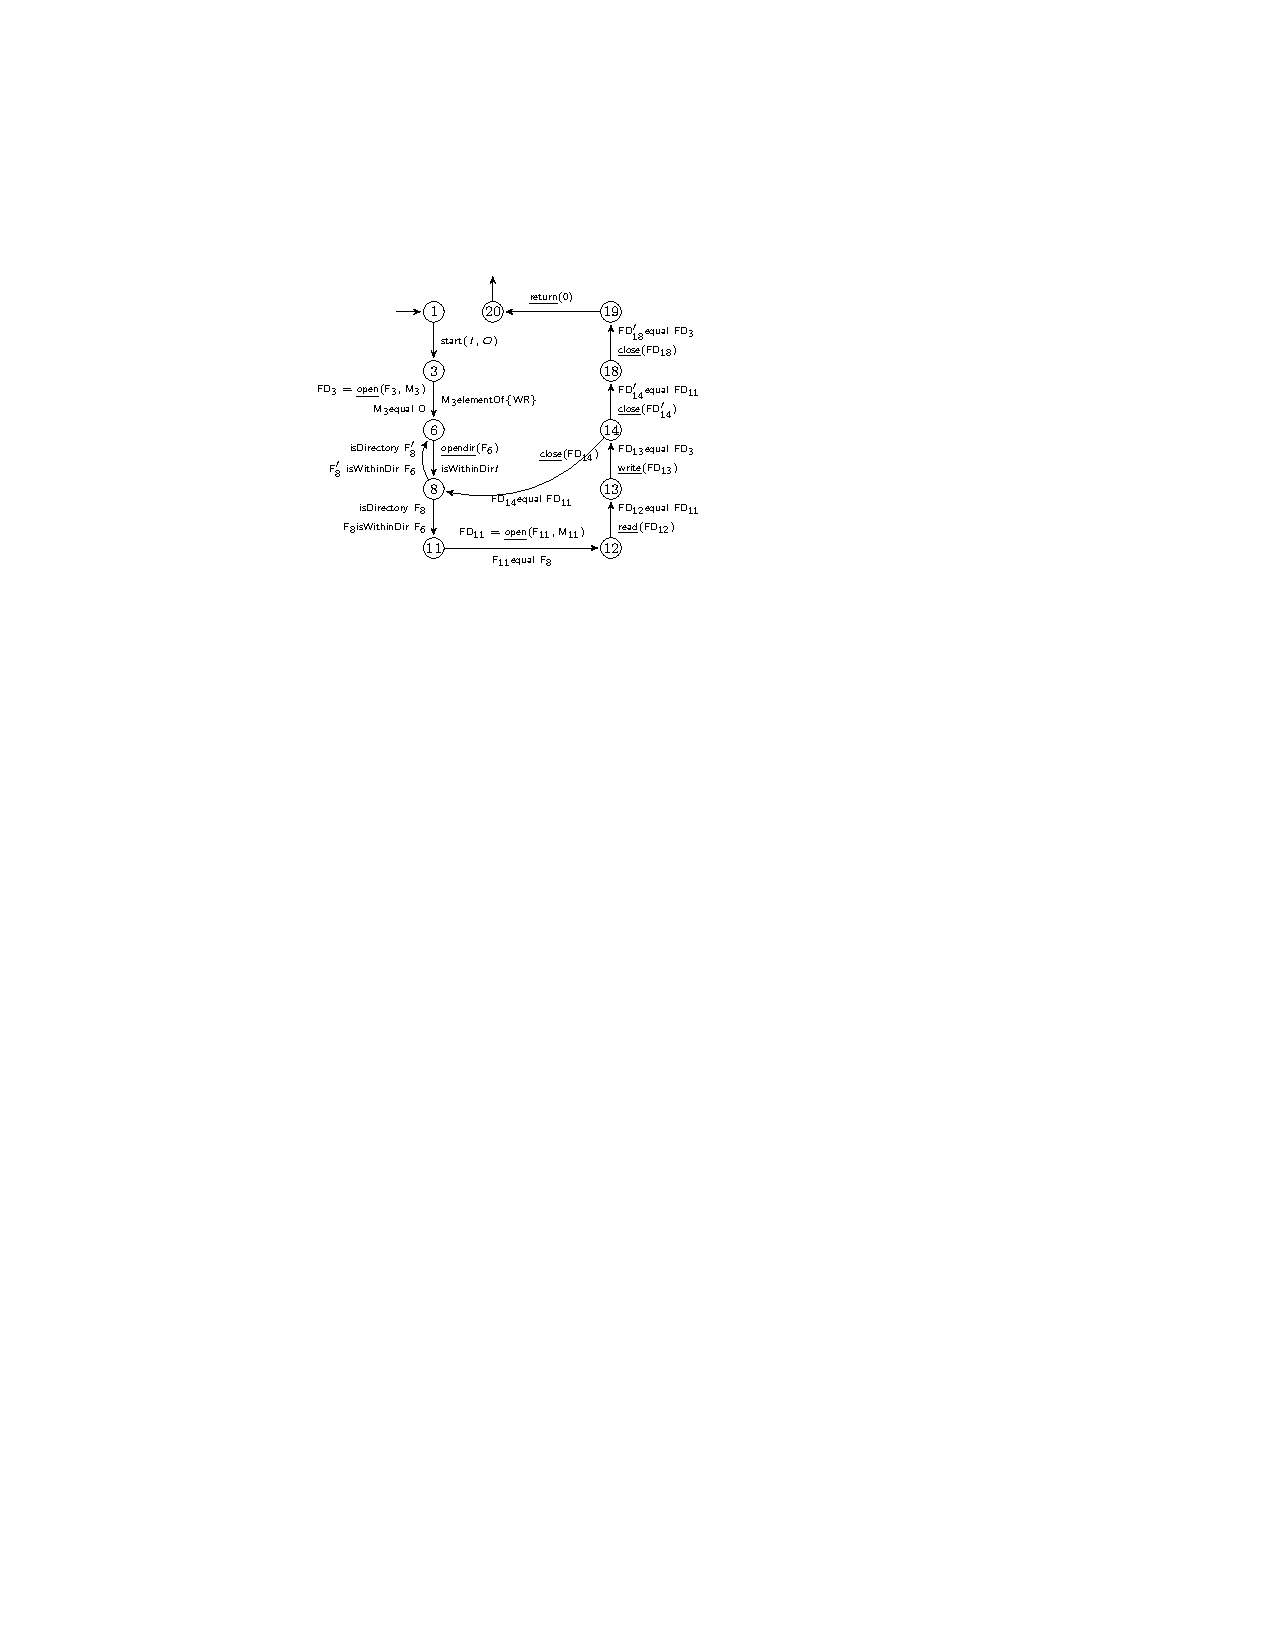
\includegraphics{figures/host/improving/rels}
      \end{flushright}
    \end{minipage}
  \end{tabular}
  \caption{A data flow example with both unary and binary relations.}
  \label{fig:rels}
\end{figure}

This knowledge is exploited in terms of \emph{unary} and \emph{binary}
relationships. For instance, if an \texttt{open} system call always
uses the same filename at the same point, a unary property can be
derived. Similarly, relationships among two arguments are supported,
by inference over the observed sequences of system calls, creating
constraints for the detection phase. Unary relationships include
\textsf{equal} (the value of a given argument is always constant),
\textsf{elementOf} (an argument can take a limited set of values),
\textsf{subsetOf} (a generalization of \textsf{elementOf}, indicating
that an argument can take multiple values, all of which drawn from a
set), \textsf{range} (specifies boundaries for numeric arguments),
\textsf{isWithinDir} (a file argument is always contained within a
specified directory), \textsf{hasExtension} (file extensions). Binary
relationships include: \textsf{equal} (equality between system call
operands), \textsf{isWithinDir} (file located in a specified
directory; \textsf{contains} is the opposite), \textsf{hasSameDirAs},
\textsf{hasSameBaseAs}, \textsf{hasSameExtensionAs} (two arguments
have a common directory, base directory or extension, respectively).

The behavior of each application is logged by storing the \ac{PID},
the \ac{PC}, along with the system calls invoked, their arguments and
returned value. The use of the \ac{PC}\index{PC} to identify the
states in the \ac{FSA}\index{FSA} stands out as an important
difference from other approaches. The \ac{PC} of each system call is
determined through \emph{stack unwinding} (i.e., going back through
the activation records of the process stack until a valid \ac{PC} is
found). The technique obviously handles process cloning and forking.

The learning algorithm is rather simple: each time a new value is
found, it is checked against all the known values of the same
type. Relations are inferred for each execution of the monitored
program and then pruned on a set intersection basis. For instance, if
relations $R_{1}$ and $R_{2}$ are learned from an execution trace
$T_{1}$ but $R_{1}$ only is satisfied in trace $T_{2}$, the resulting
model will not contain $R_{2}$. Such a process is obviously prone to
\acp{FP}\index{FP} if the training phase is not exhaustive, because
invalid relations would be kept instead of being discarded. Figure
\ref{fig:rels} shows an example (due to \citep{venkat_dataflow}) of
the final result of this process. During detection, missing
transitions or violations of properties are flagged as alerts. The
detection engine keeps track of the execution over the learned
\ac{FSA}\index{FSA}, comparing transitions and relations with what
happens, and raising an alert if an edge is missing or a constraint is
violated.

This \ac{FSA}\index{FSA} approach is promising and has interesting
features especially in terms of detection capabilities. On the other
hand, it only takes into account relationships between different types
of arguments. Also, the set of properties is limited to pre-defined
ones and totally deterministic. This leads to a possibly incomplete
detection model potentially prone to false alerts. In Section
\ref{host:improving} we detail how our approach improves the original
implementation.

Another approach based on the analysis of system calls
is~\citep{1352621}. In principle, the system is similar to the
behavior-based techniques we mentioned before. However, the authors
have tried to overcome two limitations of the learning-based
approaches which, typically, have high \acp{FPR} and require a quite
ample training set. This last issue is mitigated by adopting a
completely different approach: instead of requiring training, the
system administrator is required to specify a set of small
whitelist-like models of the desired behavior of a certain
application. At runtime, these models are evolved and adapted to the
particular context the protected application runs into; in particular,
the system exploits taint analysis to update a system call model
on-demand. This system can offer very high levels of protection but
the effort required to specify the initial model may not be so
trivial; however, the effort may be worth for mission-critical
applications on which customized hardening would be needed anyways.

\subsection{Web-based techniques}
\label{detection:ad:web} A survey of the latest (i.e., proposed
between 2003 and 2009) host-based detection approaches is provided in
this section. All the techniques included in the following are based
on \ac{HTTP}\index{HTTP}, meaning that models of normal activity are
constructed either by inspecting the decoded network frames up to the
\ac{HTTP}\index{HTTP} layer, or by acting as reverse
\ac{HTTP}\index{HTTP} proxies.

In Table \ref{tab:web-sota-taxonomy} the selected approaches are
marked with bullets to highlight their specific characteristics. Such
characteristics are based on our analysis and experience, thus, other
classifications may be possible. They are defined as follows:

\begin{description}
\item[Adaptive] refers to the capability of self-adapting to
variations in the normal behavior.
\item[Stochastic] means that stochastic techniques are exploited to
create models. For example, the model of normal \ac{HTTP}\index{HTTP}
requests may be constructed by estimating the sample mean and variance
of certain features (e.g., length of the string parameters contained
in a POST request).
\item[Deterministic] means that certain features are modeled following
a deterministic approach. For example, normal \ac{HTTP}\index{HTTP}
sessions may be only those that are generated by a certain finite
state machine.
\item[Comprehensive] approaches are those that have been extensively
developed and, in general, incorporate a rich set of features, beyond
the proof-of-concept.
\item[Response] indicates that \ac{HTTP}\index{HTTP} responses are
modeled along with \ac{HTTP}\index{HTTP} requests. For instance,
normal \ac{HTTP}\index{HTTP} responses may be modeled with the average
number of \texttt{<script />} nodes found in the response body.
\item[Session] indicates that the concept of web application session
is taken into account. For example, normal \ac{HTTP}\index{HTTP}
interactions may be modeled with the sequences of paths corresponding
to a stream of \ac{HTTP}\index{HTTP} requests.
\item[Data] indicates that parameters (i.e., GET and POST variables)
contained into \ac{HTTP}\index{HTTP} requests are modeled. For
example, normal \ac{HTTP}\index{HTTP} request may be modeled as the
cardinality of string parameters in each request.
\end{description}

Our contributions are included in Table \ref{tab:web-sota-taxonomy}
and detailed in Chapter~\ref{web}. Note that, since recent research
have experimented with several techniques and algorithms, mixed
approaches exist and often lead to better results.

\begin{sidewaystable}
  \renewcommand{\arraystretch}{1.5} \centering
  \begin{tabular}{rccccccc}
    \toprule
    
    \textsc{Approach} & \textsc{Adaptive} &
    \textsc{Stochastic} & \textsc{Deterministic} & \textsc{Comprehen.}
    & \textsc{Response} & \textsc{Session} & \textsc{Data} \\

    \midrule

    \citep{cho:cs2004:anomaly} & & $\bullet$ & & & & $\bullet$ & \\

    \citep{kruegel:jcn2005:webanomaly} & & $\bullet$ & & $\bullet$ & &
    & $\bullet$ \\

    \citep{ingham:2007:dfa} & & & $\bullet$ & & & $\bullet$ & $\bullet$ \\
    
    \citep{masibty} & & $\bullet$ & & $\bullet$ & $\bullet$ & $\bullet$ & $\bullet$ \\


    \citep{song2009smm} & & $\bullet$ & & & & & $\bullet$ \\


    \textbf{\citep{2009_maggi_robertson_kruegel_vigna}}
                                          & $\bullet$ & & $\bullet$ &
    & $\bullet$ & $\bullet$ & $\bullet$ \\


    \textbf{\citep{2009_robertson_maggi_kruegel_vigna}} & $\bullet$ & $\bullet$ & &
    & & & $\bullet$ \\

    \bottomrule
  \end{tabular}
  \caption{Taxonomy of the selected state of the art approaches for
  web-based anomaly detection. Our contributions are highlighted.}
  \label{tab:web-sota-taxonomy}
\end{sidewaystable}

Anomaly-based detectors specifically designed to protect web
applications are relatively recent. They have been first proposed
in~\citep{cho:cs2004:anomaly}, where a system to detect anomalies in
web application sessions is described. Like most of the approaches in
the literature, this technique assumes that malicious activity
expresses itself in the parameters found into \ac{HTTP}\index{HTTP}
requests. In the case of this tool, such data is parsed from the
access logs. Using Bayesian technique to assign a probability score to
the $k$-sequences ($k = 3$ in the experiments) of requested resources
(e.g., \texttt{/path/to/page}), the system can spot out unexpected
sessions. Even though this approach has been poorly evaluated, it
proposed the basic ideas on which the current research is still based.

The first technique to accurately model the normal behavior of web
application parameters is described
in~\citep{kruegel:jcn2005:webanomaly}. This approach is implemented in
\webanomaly, a tool that can be deployed in real-world scenarios. In
some sense, \webanomaly \citep{webanomalysite} is the adaptation of
\LibAnomaly models to capture the normal features of the interaction
between client and server-side applications through the
\ac{HTTP}\index{HTTP} protocol. Instead of modeling a system call and
its arguments, the same models are mapped onto resources and their
parameters (e.g., \texttt{?p=1\&show=false}). Obviously, parameters
are the focus of the analysis which employs string lenght models,
token finder models, and so forth; in addition, sessions features are
captured as well in terms of sequences of resources. In recent
versions of the tools, \webanomaly incorporated models of
\ac{HTTP}\index{HTTP} responses similar to those described
in~\citep{masibty} (see Section~\ref{web:intro:masibty}). Besides the
features shared with~\citep{kruegel:jcn2005:webanomaly}, the approach
models the \ac{DOM}\index{DOM} to enhance the detection capabilities
against \ac{SQL} injection and \ac{XSS} attacks. In Section
\ref{web:conceptdrift} an approach that exploit \ac{HTTP}\index{HTTP}
responses to \emph{detect changes} and update \emph{other} anomaly
models is described.

The approach described in \citep{ingham:2007:dfa} learns deterministic
models, \ac{FSA}, of \ac{HTTP}\index{HTTP} requests. The idea of
extracting resources and parameters is similar to that described in
\citep{kruegel:jcn2005:webanomaly}. However, instead of adopting
sophisticated models such as \ac{HMM} to encode strings' grammar, this
system applies drastic reductions to the parameters values. For
instance, dates are mapped to $\{0,1\}$ where 1 indicates that the
format of the date is known, 0 otherwise; filenames are replaced with
either a length or the extension, if the file-type is known; and so
forth. For each request, the output of this step is a list of tokens
that represent the states of the \ac{FSA}. Transitions are labeled
with the same tokens by processing them in chronological order (i.e.,
as they appear in the request). In some sense, this approach can be
considered a porting to the web domain of the techniques used to model
process behavior by means of \ac{FSA}
\citep{wagner:sp2001:staticanalysis,venkat_dataflow}.

A tool to protect against code-injection attacks has been recently
proposed in~\citep{song2009smm}. The approach exploits a mixture of
Markov chains to model legitimate payloads at the
\ac{HTTP}\index{HTTP} layer. The computational complexity of $n$-grams
with large $n$ is solved using Markov chain factorization, making the
system algorithmically efficient.

\section{Relevant Alert Correlation Techniques}
\label{detection:correlation} A survey of the latest (i.e., proposed
between 2001 and 2009) alert correlation approaches is provided in
this section.

In Table \ref{tab:correlation-sota-taxonomy} the selected approaches
are marked with bullets to highlight their specific
characteristics. Such characteristics are based on our analysis and
experience, thus, other classifications may be possible. They are
defined as follows:

\begin{description}
\item[Formal] means that formal methods are used to specify rigorous
models used in the correlation process. For instance, the relations
among alerts are specified by means of well defined first-order logic
formulae.
\item[Verification] means that the success of each alert is taken into
account. For instance, all the alerts related to attacks against port
80 are discarded if the target system does not run
\ac{HTTP}\index{HTTP} services.
\item[Stochastic] means that stochastic techniques are exploited to
create models. For example, statistic hypothesis tests may be used to
decide correlation among stream of alerts.
\item[Comprehensive] approaches are those that have been extensively
developed and, in general, incorporate a rich set of features, beyond
the proof-of-concept.
\item[Time] refers to the use of \emph{timestamp} information
extracted from alerts. For example, alerts streams may be modeled as
time series.
\item[Impact] refers to techniques that take into account the impact
(e.g., the cost) of handling alerts. For instance, alerts regarding
non-business critical machines are marked low priority.
\item[Clustering] refers to the use of clustering (and subsequent
classification) techniques. For instance, similar alerts can be
grouped together by exploiting custom distance metrics.
\end{description}

Our contributions are included in Table
\ref{tab:correlation-sota-taxonomy} and are detailed in Chapter
\ref{correlation}. Note that, since recent research have experimented
with several techniques and algorithms, mixed approaches exist and
often lead to better results.

\begin{sidewaystable}
  \renewcommand{\arraystretch}{1.5}
  \begin{tabular}{rccccccc}
    \toprule \textsc{Approach} & \textsc{Formal} & \textsc{Verif.} &
    \textsc{Comprehen.} & \textsc{Time} & \textsc{Stochastic} &
    \textsc{Clustering} & \textsc{Impact} \\

 \midrule
    \citep{herve-debar} & $\bullet$ & & & & & & \\

    \citep{valdes:raid2001:correlation} & & & & & $\bullet$ & & \\

    \citep{impactcorrelation} & & & & & & & $\bullet$ \\

    \citep{mirador} & & & $\bullet$ & & & $\bullet$ & \\

    \citep{morinmdd02} & $\bullet$ & & & & & & \\

    \citep{episodic_rule} & & & & & & $\bullet$ & \\

    \citep{dblp:conf/raid/qinl03} & & & & $\bullet$ & $\bullet$ &
    $\bullet$ & \\

    \citep{valeur04comprehensive} & & $\bullet$ &
    $\bullet$ & $\bullet$ & & & \\

    \citep{kruegel:dimva2004:verification} & & $\bullet$ & & & & & \\

    \citep{me-alert} & & & & $\bullet$ & $\bullet$ & & \\

    \textbf{\citep{MaggiZaneroRAID07}} & & & & $\bullet$ & $\bullet$ &
    & \\

    \citep{martinez:acsac2008:clustering} & & & & & $\bullet$ &
    $\bullet$ & \\

    \textbf{\citep{2009_maggi_zanero_matteucci_fusion}}&& & &
    $\bullet$ & & & \\

 \bottomrule
\end{tabular}

\caption{Taxonomy of the selected state of the art approaches for
  alert correlation. Our contributions are highlighted. Our
  contributions are highlighted.}

\label{tab:correlation-sota-taxonomy}
\end{sidewaystable}

A deterministic intrusion detection technique adapted for alert
correlation is shown in \citep{STATL}. The use of finite state
automata enables for complex scenario descriptions, but it requires
known scenarios signatures. It is also unsuitable for pure anomaly
detectors which cannot differentiate among different types of
events. Similar approaches, with similar strengths and shortcomings
but different formalisms, have been tried with the specification of
pre- and post-conditions of the attacks \citep{jigsaw}, sometimes
along with time-distance criteria \citep{ning04techniques}. It is
possible to mine scenario rules directly from data, either in a
supervised \citep{dain-fusing} or unsupervised \citep{episodic_rule}
fashion.

Statistical techniques have been also proposed, for instance
E\-ME\-RALD implements an alert correlation engine based on
probabilistic distances \citep{valdes:raid2001:correlation} which
relies on a set of similarity metrics between alerts to fuse ``near''
alerts together. Unfortunately, its performance depends on appropriate
choice of weighting parameters.

The best examples of algorithms that do not require such features are
based on time-series analysis and modeling. For instance,
\citep{me-alert} is based on the construction of time-series by
counting the number of alerts occurring into sampling intervals; the
exploitation of trend and periodicity removal algorithms allows to
filter out predictable components, leaving \emph{real} alerts only as
the output. More than a correlation approach, this is a false-positive
and noise-suppression approach, though.

In \citep{dblp:conf/raid/qinl03} an interesting algorithm for alert
correlation which seems suitable also for anomaly-based alerts is
proposed. Alerts with the same feature set are grouped into
collections of time-sorted items belonging to the same ``type''
(following the concept of type of \citep{me-alert}). Subsequently,
frequency time series are built, using a fixed size sliding-window:
the result is a time-series for each collection of alerts. The
prototype then exploits the \ac{GCT}\index{GCT} \citep{chickegg}, a
statistical hypothesis test capable of discovering causality
relationships between two time series when they are originated by
linear, stationary processes. The \ac{GCT}\index{GCT} gives a
stochastic measure, called \ac{GCI}, of how much of the history of one
time series (the supposed cause) is needed to ``explain'' the
evolution of the other one (the supposed consequence, or target). The
\ac{GCT}\index{GCT} is based on the estimation of two models: the
first is an \ac{AR} model, in which future samples of the target are
modeled as influenced only by past samples of the target itself; the
second is an \ac{ARMAX} model, which also takes into account the
supposed cause time series as an exogenous component. A statistical
F-test built upon the model estimation errors selects the best-fitting
model: if the \ac{ARMAX}\index{ARMAX} fits better, the cause
effectively influences the target.

In \citep{dblp:conf/raid/qinl03} the unsupervised identification of
causal relationships between events is performed by repeating the
above procedure for each couple of time-series. The advantage of the
approach is that it does not require prior knowledge (even if it may
use attack probability values, if available, for an optional
prioritization phase). However, in Section~\ref{correlation} we show
that the \ac{GCT}\index{GCT} fails however in recognizing
``meaningful'' relationships between \ac{IDEVAL}\index{IDEVAL}
attacks.

Techniques based on the reduction of \acp{FP}\index{FP} in anomaly
detection systems has also been studied
in~\citep{martinez:acsac2008:clustering}. Similar behavioral profiles
for individual hosts are grouped together using a $k$-means clustering
algorithm. However, the distance metric used was not explicitly
defined. Coarse network statistics such as the average number of hosts
contacted per hour, the average number of packets exchanged per hour,
and the average length of packets exchanged per hour are all examples
of metrics used to generate behavior profiles. A voting scheme is used
to generate alerts, in which alert-triggering events are evaluated
against profiles from other members of that cluster. Events that are
deemed anomalous by all members generate alerts.

Last, as will be briefly explained in Chapter~\ref{correlation}, the
alert correlation task may involve alert verification, i.e., before
reporting an alert, a procedure is run to \emph{verify} whether or not
the attack actually left some traces or, in general, had some
effect. For example, this may involve checking whether a certain
\ac{TCP} port, say, 80, is open; if not, all alerts regarding attacks
against the protected \ac{HTTP} server may be safely discarded, thus
reducing the \ac{FPR}. Although an alert correlation system would
benefit from such techniques, we do not review them, since our focus
is on the actual \emph{correlation} phase, i.e., recognizing
\emph{related} events, rather than pruning uninteresting events. The
interested reader may refer to a recent work~\citep{1349438} that,
beside describing an implementation of a novel verification system,
introduces the alert verification problem and provides a comprehensive
review of the related work.

\section{Evaluation Issues and Challenges}
\label{detection:evaluation:issues} The evaluation of
\acp{IDS}\index{IDS} is \emph{per s\'e} an open, and very difficult to
solve, research problem. Besides two attempts of proposing a rigorous
methodology for \ac{IDS} evaluation
\citep{puketza96methodology,puketza97software}, there are no standard
guidelines to perform this task. This problem is magnified by the lack
of a reliable source of test data, that is a well-known
issue. However, building a dataset to conduct repeatable experiments
is clearly a very difficult task because it is nearly impossible to
reproduce the activity of a real-world computer infrastructure. In
particular:

\begin{itemize}
\item for \emph{privacy reasons}, researchers cannot audit an
infrastructure and collect arbitrary data; in the best case, the use
of obfuscation and anonymization\index{anonymization} of the payload (e.g., character
substitution on text-based application protocol) to protect the
privacy, produces unrealistic content that will make inspection
techniques adopted by many \ac{IDS} to fail. For instance, changes in
the syntax and lexicon of strings have negative consequences for
models such as the character distribution estimator described in
Example~\ref{ex:character-distribution-model}.
\item System activity collected from real-world infrastructures
inevitably contain intrusions and not all of them are known in advance
(i.e., 0-day attacks); this makes the generation of a \emph{truth
file} a very difficult task. To workaround this problem, it is a
common practice to filter out known attacks using misuse-based systems
such as \textsf{Snort} and use the alert log as the truth
file. Unfortunately, this implicitly assumes that the chosen
misuse-based system is the baseline of the evaluation (i.e., the best
tool). On the other hand, anomaly-based systems are supposed to detect
unknown attacks; thus, using the alert log as the truth file makes the
evaluation of such systems completely meaningless.
\item In the past, two attempts have been made to simulate the user
activity on a comprehensive computer infrastructure, i.e., a military
computer network, to collect clean, background audit data to train
\acp{IDS}\index{IDS} based on unsupervised learning techniques. Even
though this ensures that the traffic contain no intrusions, the
approach has been shown to have at least two types of
shortcomings. The first is described in Section
\ref{detection:evaluation:darpa}. The second problem is that, the
attacks included (labeled in advance) do once again represent only
known attacks since the exploits are taken from public
repositories. Thus, \acp{IDS}\index{IDS} cannot be tested against
realistic intrusions such as custom attacks against proprietary and
never-exploited-before systems.
\end{itemize}

Attempts to partially solve these issues can be divided into two
groups. Some approaches proposes automated mechanisms to
\emph{generating} testing datasets, while other concentrate on the
\emph{methodologies} used to perform the evaluation task. Notably, in
\citep{cretu:sp2008:sanitization} a traffic sanitization procedure is
proposed in order to clean the background traffic; however, it is not
clear to what extent this method is substantially different from
running an arbitrary anomaly-based \ac{IDS} to filter out
attacks. Examples of publicly available, but obsolete or unreliable,
datasets are
\citep{ideval_1998_results,ideval_1999_doc,shmoosite,exploittree,kddcup}:
as exemplified by the critique described in the next section, however,
all these dataset are either unusable because of their lack of a
\emph{truth file} or are extremely biased with respect to the real
world. Among the methodological approaches,
\citep{vigna:ccs2004:sploit} proposes a tool to automatically test the
effectiveness of evasion techniques based on mutations of the
attacks. Instead, \citep{lee:2001:measures} proposes alternative
metrics to evaluate the detection capabilities,
\citep{dblp:conf/raid/sharifsgl07} focuses on the evaluation issues in
the case of host-based \acp{IDS}\index{IDS} and defines some criteria
to correctly calculate their accuracy.

Recently, probably inspired by \citep{shmoosite}, the research is
moving toward mechanisms to instrument large computer security
exercises \citep{Augustine_cyberdefense} and contests such as the
DEFCON \ac{CTF}\index{CTF}\footnote{Details available at
\url{www.defcon.org}} with the goal of collecting datasets to test
\ac{IDS}. The most up-to-date example is \citep{cdx2009}, which
describes the efforts made to collect the public dataset available at
\citep{cdx2009_site}. This dataset have the advantage of containing a
rich variety of attacks including 0-days and custom, unpublished
exploits. However, because of the aforementioned reasons, this
approach fails once again on the labeling phase since \textsf{Snort}
is used to generate the truth file. A side question is to what extent
the background traffic represent the real activity on the Internet. In
fact, since the competition was run in the controlled environment of a
private network, the users tend to behave in a different way, not to
mention that most of the participants are experienced computer users.

\subsection{Regularities in audit data of IDEVAL}
\label{detection:evaluation:darpa} \ac{IDEVAL}\index{IDEVAL} is
basically the only dataset of this kind which is freely available
along with truth files; in particular we used the 1999 dataset
\citep{ideval_1999_doc}. These data are artificially generated and
contain both network and host auditing data. A common question is how
realistic these data are. Many authors already analyzed the network
data of the 1999 dataset, finding many shortcomings
\citep{mchugh:2000:testing, Analysis1999DARPA}. Our own analysis,
published in \citep{10.1109/TDSC.2008.69}, of the 1999 host-based
auditing data revealed that this part of the dataset is all but immune
from problems. The first problem is that in the training datasets
there are too few execution instances for each software, in order to
properly model its behavior, as can be seen in
Table~\ref{tab:open-perc}. Out of (just) 6 programs present, for two
(\texttt{fdformat}\index{fdformat} and \texttt{eject}), only a handful
of executions is available, making training unrealistically simple.

The number of system calls used is also extremely limited, making
execution flows very plain. Additionally, most of these executions are
similar, not covering the full range of possible execution paths of
the programs (thus causing overfitting\index{overfitting} of any
anomaly model). For instance, in Figure \ref{fig:exectelnet} we have
plotted the frequency of the length (in system calls) of the various
executions of \texttt{telnetd}\index{telnetd} on the training data. The natural
clustering of the data in a few groups clearly shows how the
executions of the program are sequentially generated with some script,
and suffer of a lack of generality.

\begin{figure}[tb]
  \centering
  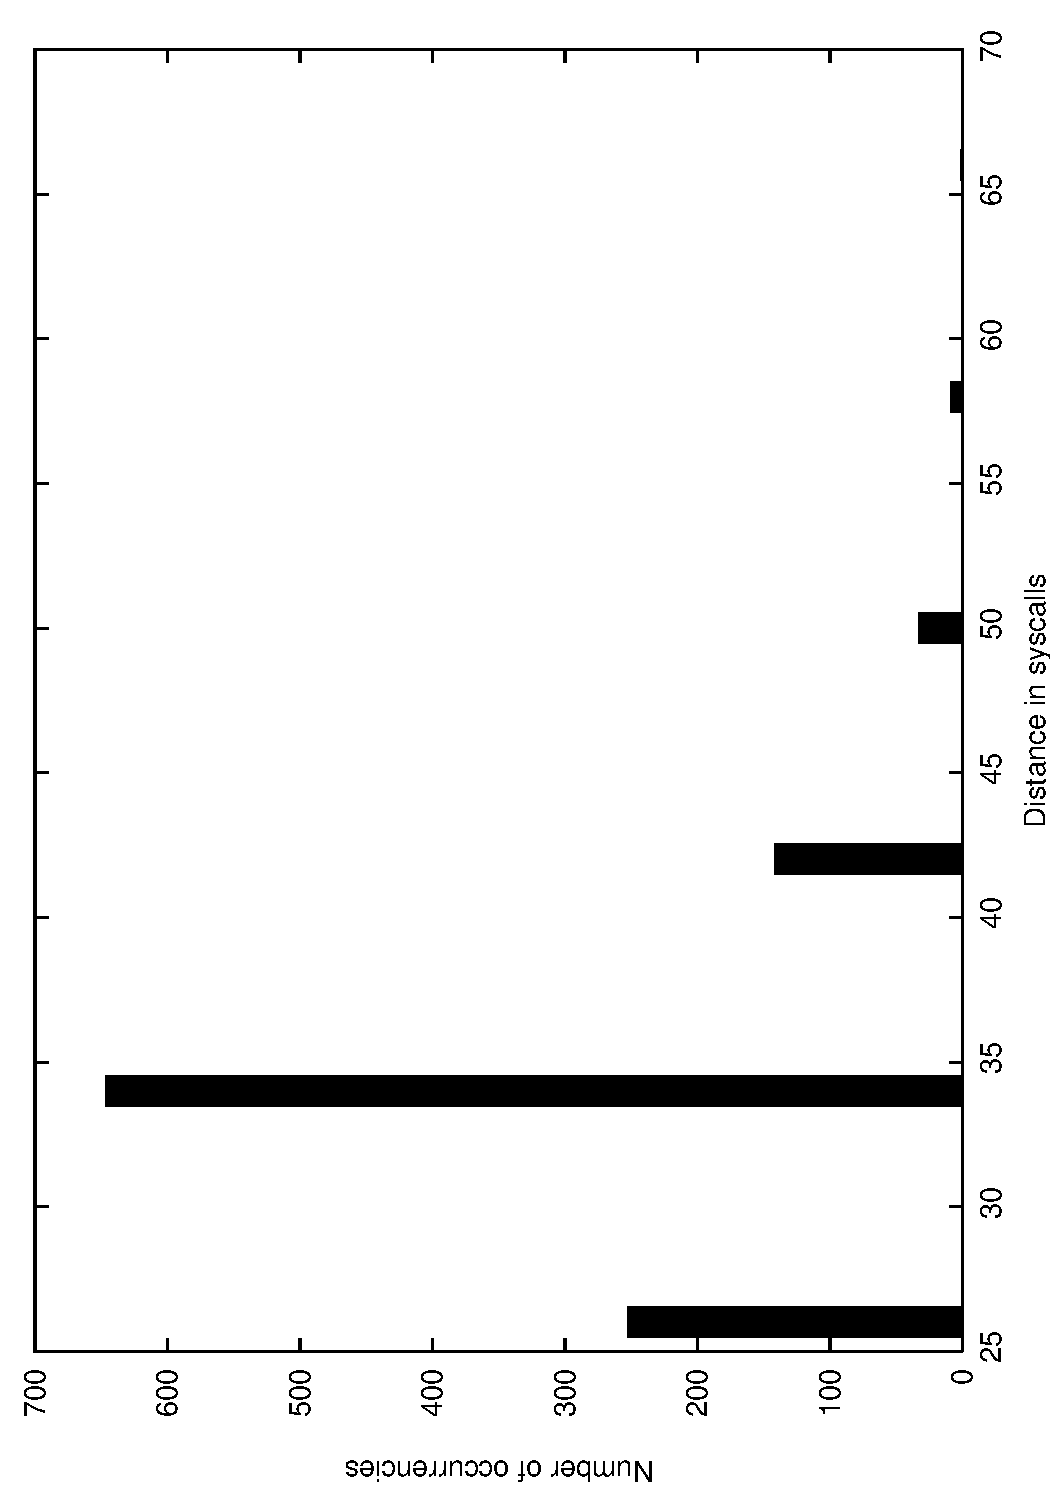
\includegraphics[angle=-90,width=.8\textwidth]{figures/host/syscall/telnet}
  \caption{\texttt{telnetd}: distribution of the number of other
  system calls among two \texttt{execve} system calls (i.e., distance
  between two consecutive \texttt{execve}).}
  \label{fig:exectelnet}
\end{figure}

System calls arguments show the same lack of variability: in all the
training dataset, all the arguments of the system calls related to
\texttt{telnetd}\index{telnetd} belong to the following set:

\begin{center}\footnotesize\ttfamily
  fork, .so.1, utmp, wtmp, initpipe, exec, netconfig,\\ service\_door,
  :zero, logindmux, pts
\end{center}

The application layer contains many flaws, too. For instance, the
\ac{FTP}\index{FTP} operations (30 sessions on the whole) use a very
limited subset of file (on average 2 per session), and are performed
always by the same users on the same files, for a limitation of the
synthetic generator of these operations. In addition, during training,
no uploads or idle sessions were performed. Command executions are
also highly predictable: for instance, one script always execute a
cycle composed of \texttt{cat}, \texttt{mail}, \texttt{mail} again,
and at times \texttt{lynx}, sometimes repeated twice. The same happens
(but in a random order) for \texttt{rm}, \texttt{sh}, \texttt{ps} and
\texttt{ls}. In addition, a number of processes have evidently crafted
names (e.g. \texttt{logout} is sometimes renamed \texttt{lockout} or
\texttt{log0ut}); the same thing happens with path names, which are
sometimes different (e.g. \texttt{/usr/bin/lynx} or
\texttt{/opt/local/bin/lynx}), but an analysis shows that they are the
same programs (perhaps symbolic links generated to create noise over
the data). The combination of the two creates interesting results such
as \texttt{/etc/loKout} or \texttt{/opt/local/bin/l0gout}. In a number
of cases, processes \texttt{lynx}, \texttt{mail} and \texttt{q} have
duplicate executions with identical \ac{PID}\index{PID} and
timestamps, and with different paths and/or different arguments; this
is evidently an inexplicable flaw of the dataset. We also found many
program executions to be curiously meaningless. In fact, the
\ac{BSM}\index{BSM} traces of some processes contain just
\texttt{execve}\index{execve} calls, and this happens for 28\% of the programs in
the testing portion dataset (especially for those with a crafted name,
like \texttt{loKout}). It is obvious that testing an host-based
\ac{IDS}\index{IDS} with one-syscall-long sequences does not make a
lot of sense, not to talk about the relevance of training against such
sequences.

An additional problem is that since 1999, when this dataset was
created, everything changed: the usage of network protocols, the
protocols themselves, the operating systems and applications used. For
instance, all the machines involved are \textsf{Solaris} version 2.5.1 hosts,
which are evidently ancient nowadays. The attacks are similarly
outdated: the only attack technique used are buffer overflows, and all
the instances are detectable in the \texttt{execve}\index{execve} system call
arguments. Nowadays attackers and attack type are much more complex
than this, operating at various layers of the network and application
stack, with a wide range of techniques and scenarios that were just
not imaginable in 1999.

To give an idea of this, we were able to create a detector which finds
all the buffer overflow attacks without any \ac{FP}: a simple script
which flags as anomalous any argument longer than 500 characters can
do this (because all the overflows occur in the parsing of the command
line, which is part of the parameters of the \texttt{execve}\index{execve} system
call which originates the process). This is obviously unrealistic.

Because of the aforementioned lack of alternatives, most existing
researches use \ac{IDEVAL}. This is a crucial factor: any bias or
error in the dataset has influenced, and will influence in the future,
the very basic research on this topic.

\subsection{The base-rate fallacy}
\label{detection:evaluation:base-rate-fallacy} The \ac{ID} is a
classification task, thus can be formalized as a Bayesian
classification problem. In particular $FPR$ and $DR$ can be defined as
probabilities. More precisely, let us define the following event
predicates:

\begin{itemize}
\item $O = $``Intrusion'', $\neg O =$``Non-intrusion'';
\item $A = $``Alert reported'', $\neg A =$``No alert reported''.
\end{itemize}

\noindent Then, we can re-write $DR$ and $FPR$ as follows.

\begin{itemize}
\item $DR = P(A \mid O)$, i.e., the probability to classify an
intrusive event as an actual intrusion.
\item $FPR = P(A \mid \neg O)$, i.e., the probability to classify a
legit event as an intrusion.
\end{itemize}

\noindent Given the above definition and the Bayes' theorem, two
measures that are more interesting than $DR$ and $FPR$ can be
calculated.

\begin{definition}[Bayesian \ac{DR}]
  The \emph{Bayesian \ac{DR}} \citep{axelsson:tissec2000:fallacy} is
  defined as:

  \begin{displaymath}
    P(O \mid A) = \frac{P(O) \cdot P(A \mid O)}{P(O) \cdot P(A \mid O)
    + P(\neg O) \cdot P(A \mid \neg O)}.
  \end{displaymath}
\end{definition}

\noindent $P(O)$ is the \emph{base-rate} of intrusions, i.e., the
probability for an intrusion to take place, regardless of the presence
of an \ac{IDS}. The Bayesian \ac{DR} not only quantifies the
probability for an alert to indicate an intrusion, it also take into
account how frequently an intrusion really happens. As pointed out by
\citep{axelsson:tissec2000:fallacy}, in this equation the $FPR = P(A
\mid \neg O)$ is strictly dominated by $P(\neg O)$. In fact, in the
real world, $P(O)$ is very low (e.g., $10^{-5}$, given two intrusions
per day, 1,000,000 audit records per day and 10 records per intrusion)
and thus $P(O) \to 1$. This phenomenon, called \emph{base-rate
fallacy}, magnifies the presence of \ac{FP}. In fact, even in the
unrealistic case of $DR = 1$, a very low $FPR = 10^{-5}$ quickly drops
the \ac{DR} to $0.0066$, which is three orders of magnitude below 1.

Besides its impact on the evaluation of an \ac{IDS}, the base-rate
fallacy has a practical impact. When inspecting the alerts log, the
security officer would indeed tend to safely ignore most of the alerts
because the past alarms have been shown to be incorrect.

\section{Concluding Remarks}
\label{detection:conclusions} In this chapter we first introduced the
basic concepts and definitions of \ac{ID}, including the most relevant
issues that arise during experimental evaluation. \ac{ID} techniques
play a fundamental role to recognize malicious activity in todays'
scenario. In particular, learning-based anomaly detection techniques
have been shown to be particularly interesting since, basically, they
implement a black-box \ac{IDS} which is easy to deploy and requires no
or scarce maintenance efforts. These systems, however, are not with
their drawbacks. From the industrial point of view, the amount of
\ac{FP} generated by anomaly-based systems is not negligible; further
exacerbating this problem is the base-rate fallacy summarized in
Section~\ref{detection:evaluation:base-rate-fallacy}. In fact, if one
considers the popularity of real attacks, even a minuscule \ac{FPR} is
magnified and instantly becomes a cost for the organization. From the
research point of view, the lack of a well-established methodology to
evaluate \ac{IDS} is an issue; in addition to this, the generation of
a reliable testing dataset is an open research problem. Todays'
evaluation is limited to two, major datasets: \ac{IDEVAL}, which,
besides being deprecated, contains several regularities that make the
evaluation extremely biased. An alternative is the modern
\ac{CDX}\index{CDX} 2009 labeled dataset collected during a security
competition; this is clearly better than \ac{IDEVAL} if ignoring the
fact that the labeling phase is consists in running
\textsf{Snort}. This inherently assumes \textsf{Snort} as the
evaluation baseline of every \ac{IDS}.

Secondly, focusing on anomaly-based techniques, we reviewed the most
recent state-of-the-art \acp{IDS}\index{IDS} to protect a host
application and a web server. We also overviewed a few approaches to
capture and analyze the network traffic as a stream of packets. This
topic is included in the reviewed literature because the contributions
in Chapter~\ref{correlation} work on alerts generated by host- and
network-based systems. Network-based \ac{IDS} are popular as they are
easy to deploy and can protect a wide range of machine (i.e., the
whole network); however, it has been shown how these systems can be
evaded by exploiting the lack of local knowledge on the single
host. The need of both global and local knowledge about a network is
probably the main motivation in favor of alert correlation
systems. The most advanced network-based anomaly detectors inspect
packet up to the \ac{TCP} layer and exploit payload clustering and
classification techniques to recognize anomalous traffic.

On the other hand, host-based systems have been shown to be effective
at detecting malicious processes on a single computer. Almost all the
reviewed approaches analyze the system calls intercepted in the
operating system kernel. Some tools known to work well for
network-based systems have been utilized in this field as well: for
instance, clustering and Bayesian classification techniques of network
packets has been adapted by several approaches to cluster similar
system calls and flag process with low Bayesian probability as
malicious, respectively. Stochastic and deterministic techniques have
been shown to be very effective. In particular, as we detail in
Section~\ref{host:improving}, deterministic models such as automata
are well suited to capture a process' control flow. On the other hand,
stochastic techniques such as character distribution or Gaussian
intervals have been show to correctly model the data flow (e.g., the
content of system call arguments) with low \ac{FP}.

Web-based \ac{ID} approaches have been overviewed as well. Although
this topic is relatively new, web-based approaches are enjoying
immense popularity. In fact, the tremendous ubiquity of the Web has
become a high-profit opportunity for the underground criminals to
spread malware\index{malware} by violating vulnerable, popular websites. The research
community have immediately recognized the relevance of this
problem. As a consequence, the industry started to adopt web-based
protection tools that have became remarkably accurate and, basically,
ready to be deployed in real-world environments.

Finally, by comparing Table~\ref{tab:network-sota-taxonomy},
\ref{tab:host-sota-taxonomy}, and \ref{tab:web-sota-taxonomy}
\emph{vs.}  \ref{tab:correlation-sota-taxonomy} it can be immediately
noticed how new this problem is. In fact, during the last decade a
common line for network-based techniques can be traced (i.e.,
exploiting payload classification). The same holds for both host-based
(i.e., the use of hybrid deterministic/stochastic techniques on system
call sequences and arguments) and web-based (i.e., the use of ensemble
of stochastic models on \ac{HTTP}\index{HTTP} parameters) techniques,
but not for alert correlation approaches. They indeed explore the use
of different techniques, but no well-established ideas can be
recognized, yet.

%%% Local Variables: 
%%% mode: latex
%%% TeX-master: "thesis"
%%% End: 

% LocalWords:  HTTPS BSM OpenBSM openbsm Cisco TCP IP webanomalysite Sourcefire
% LocalWords:  snortrules mutz syscalls timestamp TTL SOM rcccccc Determ phad
% LocalWords:  protocolanom ramadas payl zanero savaresi tokenized IDEVAL DNS
% LocalWords:  ideval LERAD datasets rulessystemcallarguments nsom NETAD ULISSE
% LocalWords:  bibbiasom smartsifter Syscall rcccccccc Comprehen libanomaly HMM
% LocalWords:  giffin venkat dataflow frossi maggi rizzo syscall anderson du na
% LocalWords:  PrivilegedProgramsMonitoring tcpdump pushdown automata stolcke
% LocalWords:  InducingProbabilisticGrammarsMerging ive FSA dir WR opendir buf
% LocalWords:  foreach isdirectory unary filename elementOf subsetOf PID smm ps
% LocalWords:  isWithinDir hasExtension hasSameDirAs hasSameBaseAs rccccccc GCT
% LocalWords:  hasSameExtensionAs masibty robertson kruegel vigna lenght Verif
% LocalWords:  filenames formulae herve impactcorrelation mirador morinmdd ning
% LocalWords:  MaggiZaneroRAID matteucci STATL dain RALD chickegg GCI ARMAX CTF
% LocalWords:  puketza anonymization shmoosite exploittree kddcup cyberdefense
% LocalWords:  DEFCON cdx DARPA fdformat telnetd execve utmp wtmp initpipe pts
% LocalWords:  netconfig logindmux logout ut loKout Solaris

\chapter{Host-based Anomaly Detection}
\label{host}
A host-based anomaly detector builds profiles of the system activity
by observing data collected on a single host (e.g., a personal
computer, a database server or a web server). By adopting learning
techniques, a host-based \ac{IDS} can automatically capture the normal
behavior of the host and flag significant deviations.

In this chapter we describe in details two contributions we proposed
to mitigate malicious activity in a POSIX-like operating system. In
both these works, our tools analyze the activity at the granularity of
the system call (e.g., \texttt{open}, \texttt{read}, \texttt{chmod})
and monitor each running process in parallel using a multi-threaded
scheduling. Our approaches integrate the most advanced techniques
that, according to the recent literature, have been shown to be
effective. We also propose novel techniques, such as clustering of
system calls to classify system calls and Markov models to capture
each process' behavior, and their refinements to further lower the
\ac{FPR}. All the systems described in this chapter have been
evaluated using both \ac{IDEVAL} and a more realistic dataset that
also includes new attacks (details on the generation of such a dataset
are described). In addition, we describe our tests on a dataset we
created through the implementation of an innovative technique of
anti-forensics, and we show that our approach yields promising results
in terms of detection. The goal of this extensive set of experiments
is to use our prototype to circumvent definitive anti-forensics
tools. Basically, we demonstrate how our tool can detect stealthy
in-memory injections of executable code, and in-memory execution of
binaries (the so-called ``userland\index{userland} exec'' technique, which we
re-implement in a reliable way).

\section{Preliminaries}
\label{host:experimental-setup}
In order to avoid the shortcomings mentioned in
Section~\ref{detection:evaluation:issues}, besides the use of
\ac{IDEVAL}\index{IDEVAL} for comparison purposes with \SyscallAnomaly
(which was tested on that dataset), we generated an additional
experimental dataset for other frequently used console
applications. We chose different buffer overflow exploits that allow
to execute arbitrary code.

More precisely, in the case of \texttt{mcweject 0.9}\index{mcweject},
the vulnerability \citep{adv-eject} is a very simple stack overflow,
caused by improper bounds checking. By passing a long argument on the
command line, an aggressor can execute arbitrary code on the system
with root privileges. There is a public exploit for the vulnerability
\citep{exp-eject} which we modified slightly to suit our purposes and
execute our own payload. The attack against
\texttt{bsdtar}\index{bsdtar} is based on a publicly disclosed
vulnerability in the PAX handling functions of \texttt{libarchive
  2.2.3} and earlier \citep{adv-libarchive}, where a function in file
\texttt{archive\_read\_support\_format\_tar.c} does not properly
compute the length of a buffer when processing a malformed PAX archive
extension header (i.e., it does not check the length of the header as
stored in a header field), resulting in a heap overflow which allows
code injection through the creation of a malformed PAX archive which
is subsequently extracted by an unsuspecting user on the target
machine. In this case, we developed our own exploit, as none was
available online, probably due to the fact that this is a heap
overflow and requires a slightly more sophisticated exploitation
vector. In particular, the heap overflow allows to overwrite a pointer
to a structure which contains a pointer to a function which is called
soon after the overflow. So, our exploit overwrites this pointer,
redirecting it to the injected buffer. In the buffer we craft a clone
of the structure, which contains a pointer to the
shellcode\index{shellcode} in place of the correct function pointer.

Our testing platform runs a vanilla installation of
\textsf{FreeBSD}\index{FreeBSD} 6.2 on a x86 machine; the kernel has
been recompiled enabling the appropriate auditing modules. Since our
systems, and other host-based anomaly detectors
\citep{libanomaly,mutz06:syscalls}, accept input in the \ac{BSM}
format, the \textsf{OpenBSM} \citep{openbsm} auditing tools collection
has been used for collecting audit trails. We have audited vulnerable
releases of \texttt{eject} and \texttt{bsdtar}\index{bsdtar}, namely:
\texttt{mcweject 0.9}\index{mcweject} (which is an alternative to the
BSD \texttt{eject}) and the version of \texttt{bsdtar}\index{bsdtar}
which is distributed with \textsf{FreeBSD}\index{FreeBSD} 6.2. During the generation
process, the audit trails keep changing, along with the simulated user
behavior. It is important to underline that normal users would never
use really random names for their files and directories, they usually
prefer to use words from their tongue plus a limited set of characters
(e.g., \texttt{.}, \texttt{-}, \texttt{\_}) for concatenating
them. Therefore, we rely on a large dictionary of words for generating
file names.

The \texttt{eject} executable has a small set of command line option
and a very plain execution flow. For the simulation of a legitimate
user, we simply chose different permutations of flags and different
devices. For this executable, we manually generated 10 executions,
which are remarkably similar (as expected).

Creating a dataset of normal activity for the \texttt{bsdtar}\index{bsdtar} program
is more challenging. It has a large set of command line options, and
in general is more complex than \texttt{eject}. While the latter is
generally called with an argument of \texttt{/dev/*}, the former can
be invoked with any argument string, for instance \texttt{bsdtar cf
  myarchive.tar /first/path /second/random/path} is a perfectly
legitimate command line. Using a procedure similar to the one used for
creating the \ac{IDEVAL}\index{IDEVAL} dataset, and in fact used also
in \citep{sekar:sp2001:automaton}, we prepared a shell script which
embeds pseudo-random behaviors of an average user who creates or
extracts archives. To avoid the regularities found in
\ac{IDEVAL}\index{IDEVAL}, to simulate user activity, the script
randomly creates random-sized, random-content files inside a snapshot
of a real-world desktop file-system. In the case of the simulation of
super-user executions, these files are scattered around the system; in
the case of a regular user, they are into that user's own home
directory. Once the file-system has been populated, the tool randomly
walks through the directory tree and randomly creates TAR
archives. Similarly, found archives are randomly expanded. The
randomization takes also into account the different use of flags made
by users: for instance, some users prefer to uncompress an archive
using \texttt{tar xf archive.tar}, many others still use the dash
\texttt{tar -xf archive.tar}, and so on.

In addition to the aforementioned datasets, we used attacks against
\texttt{sing}, \texttt{mt-daapd}, \texttt{proftpd}, \texttt{sudo}, and
\texttt{BitchX}. To generate clean training data we followed similar
randomization and scripting mechanisms described previously.

Specifically, \texttt{sing} is affected by CVE-2007-6211, a
vulnerability which allows to write arbitrary text on arbitrary files
by exploiting a combination of parameters. This attack is meaningful
because it does not alter the control flow, but just the data flow,
with an \texttt{open} which writes on unusual files. Training datasets
contain traces of regular usage of the program invoked with large sets
of command line options.

\texttt{mt-daapd} is affected by a format string vulnerability
(CVE-2007-5825) in \texttt{ws\_addarg()}. It allows remote execution
of arbitrary code by including the format specifiers in the username
or password portion of the base64-encoded data on the
\texttt{Authorization: Basic} \ac{HTTP}\index{HTTP} header sent to
\texttt{/xml-rpc}. The \texttt{mod\_ctrls} module of \texttt{proftpd}
let local attackers to fully control the integer \texttt{regarglen}
(CVE-2006-6563) and exploit a stack overflow to gain root privileges.

\texttt{sudo} does not properly sanitize data supplied through
\texttt{SHELLOPTS} and \texttt{PS4} environment variables, which are
passed on to the invoked program (CVE-2005-2959). This leads to the
execution of arbitrary commands as privileged user, and it can be
exploited by users who have been granted limited superuser
privileges. The training set includes a number of execution of
programs commonly run through sudo (e.g., \texttt{passwd},
\texttt{adduser}, editing of \texttt{/etc/} files) by various users
with different, limited superuser privileges, along with benign traces
similar to the attacks, invoked using several permutations of option
flags.

\texttt{BitchX} is affected by CVE-2007-3360, which allows a remote
attacker to execute arbitrary commands by overfilling a hash table and
injecting an EXEC hook function which receives and executes shell
commands. Moreover, failed exploit attempts can cause DoS. The
training set includes several \ac{IRC}\index{IRC} client sessions and
a legal \ac{IRC}\index{IRC} session to a server having the same
address of the malicious one.

\begin{note}
  First, it is important to underline that the scripts that we
  prepared to set up the experiments are only meant to generate the
  system calls that are generated when a particular executable is
  stimulated with different command line options and different
  inputs. By no means we claim that such scripts can emulate a user's
  overall activity. Although the generation of large dataset for
  \ac{IDS} evaluation goes beyond the scope of our work, these scripts
  attempt to reflect the way a regular user invokes \texttt{tar} or
  \texttt{eject}; this was possible because they are both simple
  programs which require a limited number of command line
  options. Clearly, generating such a dataset for more sophisticated
  applications (e.g., a browser, a highly-interactive graphic tool)
  would be much more difficult.

  Secondly, we recall that these scripts have been set up \emph{only}
  for collecting clean data. Such data collection is not needed by our
  system when running, since the user data would be already available.
\end{note}

In \citep{venkat_dataflow} a real web and \ac{SSH}\index{SSH} server
logs were used for testing. While this approach yields interesting
results, we did not follow it for three reasons. Firstly, in our
country various legal concerns limit what can be logged on real-world
servers. In second place, \ac{HTTP}\index{HTTP} and
\ac{SSH}\index{SSH} are complex programs where understanding what is
correctly identified and what is not would be difficult (as opposed to
simply counting correct and false alerts). Finally, such a dataset
would not be reliable because of the possibility of the presence of
real attacks inside the collected logs (in addition to the attacks
inserted manually for testing).

\section{Malicious System Calls Detection}
\label{host:syscall}
In this section we describe our contribution regarding anomaly
detection of host-based attacks by exploiting unsupervised system
calls arguments and sequences \citep{10.1109/TDSC.2008.69}. Analyzing
both the theoretical foundations described in
\citep{libanomaly,mutz06:syscalls}, and the results of our tests, we
proposed an alternative system, which improves some of the ideas of
\SyscallAnomaly (the \ac{IDS} developed on top of \LibAnomaly) along
with clustering, Markov based modeling, and behavior
identification. The approach is implemented in a prototype called
\ac{SSAADE}, written in \ac{ANSI}\index{ANSI} C. A set of anomaly
detection models for the individual parameters of the calls is
defined. Then, a clustering process which helps to better fit models
to system call arguments, and creates inter-relations among different
arguments of a system call is defined by means of ad-hoc distance
metrics. Finally, we exploit Markov models to encode the monitored
process' normal behavior. The resulting system needs no prior
knowledge input; it has a good \ac{FPR}, and it is also able to
correctly contextualize alarms, giving the security officer more
information to understand whether a \ac{TP} or \ac{FP} happened, and
to detect variations over the entire execution flow, as opposed to
punctual variations over individual instances.

\ac{SSAADE} uses the sequence as well as the parameters of the system
calls executed by a process to identify anomalous behaviors. As
detailed in Section~\ref{detection:ad:host}, the use of system calls
as anomaly indicators is well established in literature (e.g. in
\citep{Self,DetClassSequences,seqsys,System-CallDelays,Ripper,stolfo,HMMDetecting,markov-simile,State-basedDetection,sekar:sp2001:automaton,wagner:sp2001:staticanalysis,giffin,ding}),
usually without handling their parameters (with the notable exceptions
of
\citep{libanomaly,rulessystemcallarguments,venkat_dataflow}). \ac{SSAADE}
is an improvement to the existing tool by means of four key novel
contributions:

\begin{itemize}
\item we build and carefully test anomaly detection models for system
  call parameters, in a similar way to \citep{libanomaly};
\item we introduce the concept of \emph{clustering} arguments in order
  to automatically infer different ways to use the same system call;
  this leads to more precise models of normality on the arguments;
\item the same concept of clustering also creates correlations among
  the different parameters of a same system call, which is not present
  in any form in
  \citep{libanomaly,rulessystemcallarguments,venkat_dataflow};
\item the traditional detector based on deviations from previously
  learned Markov models is complemented with the concept of
  clustering; the sequence of system calls is transformed into a
  sequence of labels (i.e., classes of calls): this is conceptually
  different than what has been done in other works (such as
  \citep{rulessystemcallarguments}), where sequences of events and
  single events by themselves are both taken into account but in an
  orthogonal way.
\end{itemize}

The resulting model is also able to correctly contextualize alarms,
providing the user with more information to understand what caused any
\ac{FP}, and to detect variations over the execution \emph{flow}, as
opposed to variations over \emph{single} system call. We also discuss
in depth how we performed the implementation and the evaluation of the
prototype, trying to identify and overcome the pitfalls associated
with the usage of the \ac{IDEVAL}\index{IDEVAL} dataset.

\subsection{Analysis of SyscallAnomaly}
\label{host:syscall:crit-libanomaly}
In order to replicate the original tests of \SyscallAnomaly, we used
the host-based auditing data in \ac{BSM}\index{BSM} format contained
in the \ac{IDEVAL}\index{IDEVAL} dataset. For now, it is sufficient to
note that we used the \ac{BSM}\index{BSM} audit logs from the system
named \texttt{pascal.eyrie.af.mil}, which runs a \textsf{Solaris}
2.5.1 operating system. Before describing the dataset used, we briefly
summarize the models used by \SyscallAnomaly: string length model, the
character distribution model, the structural inference model and the
token search model.

\begin{description}

\item [string length model] --- computes, from the strings seen in the
  training phase, the sample mean $\mu$ and variance $\sigma^2$ of
  their lengths. In the detection phase, given $l$, the length of the
  observed string, the likelihood $p$ of the input string length with
  respect to the values observed in training is equal to one if $l <
  \mu + \sigma$ and $\frac{\sigma^2}{(l-\mu)^2}$ otherwise.

\item [character distribution model] --- analyzes the discrete
  probability distribution of characters in a string. Each string is
  considered as a set of characters, which are inserted into an
  histogram, in decreasing order of occurrence, with a classical rank
  order/frequency representation. For detection, a $\chi^2$ Pearson
  test returns the likelihood that the observed string histogram comes
  from the learned model.

\item [structural inference model] --- learns the structure of
  strings, that are first simplified using the following translation
  rules: \texttt{[A-Z]} $\to$ \texttt{A}, \texttt{[a-z]} $\to$
  \texttt{a}, \texttt{[0-9]} $\to$ \texttt{0}. Finally, multiple
  occurrences of the same character are simplified. For instance,
  \texttt{/usr\-/lib\-/libc\-.so} is translated into
  \texttt{/aaa\-/aaa\-/aaaa\-.aa}, and further compressed into
  \texttt{/a/a/a.a}. A probabilistic grammar encoded in a
  \acf{HMM}\index{HMM} is generated by exploiting a Bayesian merging
  procedure, as described in
  \citep{stolcke93hidden,stolcke:icsi1994:merging,InducingProbabilisticGrammarsMerging}.
  
\item [token search model] --- applied to arguments which contain
  flags or modes. This model uses a statistical test to determine
  whether or not an argument contains a finite set of values. The core
  idea (drawn from \citep{lee-learning}) is that if the set is finite,
  then the number of different arguments in the training set will grow
  in a much slower way than the total number of samples. This is
  tested using a Kolgomorov-Smirnov non parametric test. If the field
  contains a set of tokens, the set of values observed during training
  is stored. During detection, if the field has been flagged as a
  token, the input is compared against the stored values list. If it
  matches a former input, the model returns 1, else it returns 0,
  without regard to the relative frequency of the tokens in the
  training data.
\end{description}

A confidence rating is computed at training for each model, by
determining how well it fits its training set; this value is meant to
be used at runtime to provide additional information on the
reliability of the model.

Returning to the analysis, we used a dataset that contains 25 buffer
overflow attacks against 4 different applications: \texttt{eject},
\texttt{fdformat}, \texttt{ps}, and \texttt{ffbconfig} (not
tested). We used data from weeks 1 and 3 for training, and data from
weeks 4 and 5 for testing the detection phase. However, it must be
noted that some attacks are not directly detectable through system
call analysis. The most interesting attacks for testing
\SyscallAnomaly are the ones in which an attacker exploits a
vulnerability in a local or remote service to allow an intruder to
obtain or escalate privileges.

In addition to the programs named above, we ran \SyscallAnomaly also
on three other programs, namely \texttt{ftpd}, \texttt{sendmail} and
\texttt{telnetd}, which are known not to be subject to any attack in
the dataset, in order to better evaluate the \ac{FPR} of the
system. In Table \ref{tab:risultatisyscallanom} we compare our results
with the released version of \SyscallAnomaly \citep{libanomalySite} to
reproduce the results reported in \citep{libanomaly}.

\begin{table}[t]
  \centering
  \begin{tabular}{lcc}
    \toprule
    \textsc{Program} & \SyscallAnomaly & \ac{SSAADE}\\
    \midrule
    \texttt{fdformat} & 0 & 1 (4)\\
    \texttt{eject} & 0 & 1 (6)\\
    \texttt{ps} & 0 & 2 (10) \\
    \texttt{ftpd} & 14 &  2 (45)\\
    \texttt{telnetd} & 17 & 2 (198) \\
    \texttt{sendmail} & 8 & 4 (97)\\
    \bottomrule
  \end{tabular}

  \caption{Comparison of \SyscallAnomaly (results taken from
    \citep{libanomaly}) and \ac{SSAADE}\index{SSAADE} in terms of number
    \acp{FP}\index{FP} on the \ac{IDEVAL}\index{IDEVAL} dataset. For
    \ac{SSAADE}\index{SSAADE}, the amount of system calls flagged as
    anomalous is reported between brackets.}
  \label{tab:risultatisyscallanom}
\end{table}

As can be seen, our results are different from those reported in
\citep{libanomaly}, but the discrepancy can be explained by a number
of factors:

\begin{itemize}
\item the version of \SyscallAnomaly and \LibAnomaly available online
  could be different from or older than the one used for the published
  tests;
\item several parameters can be tuned in \SyscallAnomaly, and a
  different tuning could produce different results;
\item part of the data in the \ac{IDEVAL}\index{IDEVAL} dataset under
  consideration are corrupted or malformed;
\item in \citep{libanomaly} it is unclear if the number of
  \acp{FP}\index{FP} is based on the number of executions erroneously
  flagged as anomalous, or on the number of anomalous syscalls\index{syscalls}
  detected.
\end{itemize}

These discrepancies make a direct comparison difficult, but our
numbers confirm that \SyscallAnomaly performs well overall as a
detector. However, \acp{FP}\index{FP} and detected anomalies are
interesting to study, in order to better understand how and where
\SyscallAnomaly fails, and to improve it. Therefore we analyzed in
depth a number of executions. Just to give a brief example, let us
consider \texttt{eject}: it is a very plain, short program, used to
eject removable media on UNIX-like systems: it has a very simple and
predictable execution flow, and thus it is straightforward to
characterize: dynamic libraries are loaded, the device
\texttt{vol@0:volctl} is accessed, and finally, the device
\texttt{unnamed\_floppy} is accessed.

\begin{table}[tb]
  \centering
  \begin{tabular}{rrl}
    \toprule
    \multicolumn{3}{c}{\textsc{True positive} (\texttt{execve})}\\
    \midrule
    file & \multicolumn{2}{l}{\texttt{/usr/bin/eject}}\\
    argv & \multicolumn{2}{l}{\texttt{eject$\backslash$0x20$\backslash$0x20$\backslash$0x20$\backslash$0x20[...]}}\\
    \cmidrule{2-3}
    & \emph{Models} & \emph{Prob. (Conf.)}\\
    \cmidrule{2-3}
    file & Token Search & 0.999999 (0)\\
    & String Length & $10^{-6}$ (0)\\
    argv & Character Distribution& 0.005 (0.928)\\
    & Structural Inference & $10^{-6}$ (0.025)\\
    \midrule
    \multicolumn{2}{r}{Total Score (Threshold)} & 1.316 (0.0012)\\
    \bottomrule
  \end{tabular}

  \vspace*{5mm}

  \begin{tabular}{rrl}
    \toprule
    \multicolumn{3}{c}{\textsc{False positive} (\texttt{open})}\\
    \midrule
    file & \multicolumn{2}{l}{\texttt{/vol/dev/rdiskette0/c0t6d0/volume\_1}}\\
    flags & \multicolumn{2}{l}{\texttt{crw-rw-rw-}}\\
    \cmidrule{2-3}
    & \emph{Models} & \emph{Prob. (Conf.)}\\
    \cmidrule{2-3}
    & String Length & 0.667 (0.005)\\
    path & Character Distribution& 0.99 (0.995)\\
    & Structural Inference & $10^{-6}$ (1)\\
    & Token Search & 0.999 (1)\\
    \midrule
    \multicolumn{2}{r}{Total Score (Threshold)} & 8.186 (1.454)\\
    \bottomrule
  \end{tabular}

  \caption{A true positive and a \ac{FP} on \texttt{eject}.}
  \label{tab:eject-exec}
\end{table}

The dataset contains only one kind of attack against \texttt{eject}:
it is a buffer overflow with command execution (see Table
\ref{tab:eject-exec}). The exploit is evident in the \texttt{execve}
system call, since the buffer overflow is exploited from the command
line. Many of the models in \SyscallAnomaly are able to detect this
problem: the character distribution model, for instance, performs
quite well. The anomaly value turns out to be 1.316, much higher than
the threshold (0.0012). The string length and structural inference
models flag this anomaly as well, but interestingly they are mostly
ignored since their confidence value is too low. The confidence value
for the token model is 0, which in \SyscallAnomaly convention means
that the field is not recognized as a token. This is actually a
shortcoming of the association of models with parameters in
\SyscallAnomaly, because the ``filename'' argument is not really a
token.

A \ac{FP} happens when a removable unit, unseen during training, is
opened (see Table \ref{tab:eject-exec}). The structural inference
model is the culprit of the false alert, since the name structure is
different from the previous one for the presence of an underscore. As
we will see later on, the extreme brittleness of the transformation
and simplification model is the main weakness of the Structural
Inference model.

\begin{table}[tb]
  \centering
  \begin{tabular}{rrl}
    \toprule
    \multicolumn{3}{c}{\textsc{True positive} (\texttt{open})}\\
    \midrule
    path & \multicolumn{2}{l}{\texttt{/usr/lib/locale/iso\_8859\_1/[...]}}\\
    flags & \multicolumn{2}{l}{\texttt{-r-xr-xr-x}}\\
    \cmidrule{2-3}
    & \emph{Models} & \emph{Prob. (Conf.)}\\
    \cmidrule{2-3}
    & String Length & 0.0096 (0.005)\\
    & Character Distribution& 0.005 (0.995)\\
    & Structural Inference & $10^{-6}$ (0.986)\\
    & Token Search & $10^{-6}$ (1)\\
    \midrule
    \multicolumn{2}{r}{Total Score (Threshold)} & 8.186 (1.454)\\
    \bottomrule
  \end{tabular}
  \caption{True positive on \texttt{fdformat} while opening a localization file.}
  \label{tab:fdformat-locale}
\end{table}

Another alert happens in the opening of a localization file (Table
\ref{tab:fdformat-locale}), which triggers the string length model and
creates an anomalous distribution of characters; moreover, the
presence of numbers, underscores and capitals creates a structure that
is flagged as anomalous by the structural inference model. The anomaly
in the token search model is due to the fact that the open mode
(\texttt{-r-xr-xr-x}) is not present in any of the training
files. This is not an attack, but is the consequence of the buffer
overflow attack, and as such is counted as a true positive. However,
it is more likely to be a lucky, random side effect.

Without getting into similar details for all the other programs we
analyzed (details which can be found in Section
\ref{detection:evaluation:darpa}), let us summarize our
findings. \texttt{ps} is a jack-of-all-trades program to monitor
process execution, and as such is much more articulated in its options
and execution flow than any of the previously analyzed
executables. However, the sequence of system calls does not vary
dramatically depending on the user specified options: besides library
loading, the program opens \texttt{/tmp/ps\_data} and the files
containing process information in \texttt{/proc}. Also in this case,
attacks are buffer overflows on a command-line parameter. In this
case, as was the case for \texttt{fdformat}, a correlated event is
also detected, the opening of file \texttt{/tmp/foo} instead of file
\texttt{/tmp/ps\_data}. Both the Token Search model and the Structural
Inference model flag an anomaly, because the opening mode is unseen
before, and because the presence of an underscore in
\texttt{/tmp/ps\_data} makes it structurally different from
\texttt{/tmp/foo}. However, if we modify the exploit to use
\texttt{/tmp/foo\_data}, the Structural Inference model goes quiet. A
\ac{FP} happens when \texttt{ps} is executed with options
\texttt{lux}, because the structural inference model finds this usage
of parameters very different from \texttt{-lux} (with a dash), and
therefore strongly believes this to be an attack. Another \ac{FP}
happens when a zone file is opened, because during training no files
in \texttt{zoneinfo} were opened. In this case it is very evident that
the detection of the opening of the \texttt{/tmp/foo} file is more of
another random side effect than a detection, and in fact the model
which correctly identifies it also creates \acp{FP}\index{FP} for many
other instances. In the case of \texttt{in.ftpd}, a common
\ac{FTP}\index{FTP} server, a variety of commands could be
expected. However, because of the shortcomings of the
\ac{IDEVAL}\index{IDEVAL} dataset detailed in Section
\ref{detection:evaluation:darpa}, the system call flow is fairly
regular. After access to libraries and configuration files, the logon
events are recorded into system log files, and a \texttt{vfork} call
is then executed to create a child process to actually serve the
client requests. In this case, the \acp{FP}\index{FP} mostly happen
because of the opening of files never accessed during training, or
with ``unusual modes''.

\texttt{sendmail} is a really complex program, with complex execution
flows that include opening libraries and configuration files,
accessing the mail queue (\texttt{/var/spool/mqueue}), transmitting
data through the network and/or saving mails on disk. Temporary files
are used, and the \texttt{setuid} call is also used, with an argument
set to the recipient of the message (for delivery to local users).

A \ac{FP} happens for instance when \texttt{sendmail} uses
\texttt{UID} 2133 to deliver a message. In training that particular
\texttt{UID} was not used, so the model flags it as anomalous. Since
this can happen in the normal behavior of the system, it is evidently
a generic problem with the modeling of \texttt{UID}s as it is done in
LibAnomaly. Operations in \texttt{/var/mail} are flagged as anomalous
because the file names are similar to \texttt{/var/mail/emonca000Sh},
and thus the alternation of lower and upper case characters and
numbers easily triggers the Structural Inference model.

We outlined different cases of failure of \SyscallAnomaly. But what
are the underlying reasons for these failures? The \emph{structural
  inference model} is probably the weakest overall. It is too
sensitive against non alphanumeric characters, since they are not
altered nor compressed: therefore, it reacts strongly against slight
modifications that involve these characters. This becomes visible when
libraries with variable names are opened, as it is evident in the
\acp{FP}\index{FP} generated on the \texttt{ps} program. On the other
hand, the compressions and simplifications introduced are excessive,
and cancel out any interesting feature: for instance, the strings
\texttt{/tmp/tempfilename} and \texttt{/etc/shadow} are
indistinguishable by the model. Another very surprising thing, as we
already noticed, is the choice of ignoring the probability values in
the Markov model, turning it into a binary value (0 if the string
cannot be generated, 1 otherwise). This assumes an excessive weight in
the total probability value, easily causing a false alarm.

\begin{table}[tb]
  \centering
  \begin{tabular}{lcc}
    \toprule
    \textsc{Executable} & \multicolumn{2}{c}{\scshape False Positives (Syscalls flagged)} \\
    \midrule
    & With the \ac{HMM}\index{HMM} & Without the \ac{HMM}\index{HMM}\\
    \cmidrule{2-3}
    \texttt{fdformat} & 1 (4) & 1(4)\\
    \texttt{eject} & 1 (6) & 1 (3)\\
    \texttt{ps} & 2 (10) & 1 (6)\\
    \texttt{ftpd} & 2 (45) & 2 (45)\\
    \texttt{telnetd} & 2 (198) & 0 (0)\\
    \texttt{sendmail} & 4 (97) & 4 (97)\\
    \bottomrule
  \end{tabular}
  \caption{Behavior of \SyscallAnomaly with and without the Structural Inference Model}
  \label{tab:excl-HMM}
\end{table}

To verify our intuition, we re-ran the tests excluding the Structural
Inference model: the \ac{DR} is unchanged, while the \ac{FPR} strongly
diminishes, as shown in Table \ref{tab:excl-HMM} (once again, both in
terms of global number of alerts, and of flagged system
calls). Therefore, the Structural Inference model is not contributing
to detection; instead it is just causing a growth in the anomaly
scores which could lead to an increased number of false positives. The
case of \texttt{telnetd} is particularly striking: excluding the
Structural Inference model makes all the false positives disappear.

The \emph{character distribution model} is much more reliable, and
contributes positively to detection. However, it is not accurate about
the particular distribution of each character, and this can lead to
possible mimicry attacks. For instance, executing \texttt{ps -[x)} has
a very high probability, because it is indistinguishable from the
usual form of the command \texttt{ps -axu}.

The \emph{token search model} has various flaws. First of all, it is
not probabilistic, as it does not consider the relative probability of
the different values. Therefore, a token with 1000 occurrences is
considered just as likely as one with a single occurrence in the whole
training set. This makes the training phase not robust against the
presence of outliers or attacks in the training dataset. Additionally,
since the model is applied only to fields that have been determined
beforehand to contain a token, the statistical test is not useful: in
fact, in all our experiments, it never had a single negative
result. It is also noteworthy that the actual implementation of this
test in \citep{libanomalySite} differs from what is documented in
\citep{libanomaly, mutz06:syscalls, lee-learning}.

Finally, the \emph{string length model} works very well, even if this
is in part due to the artifacts in the dataset, as we describe in
Section~\ref{detection:evaluation:darpa}.

\subsection{Improving \SyscallAnomaly}
\label{host:syscall:our-proposal}
We can identify and propose three key improvements over
\SyscallAnomaly. Firstly, we redesign improved models for anomaly
detection on arguments, focusing on their reliability. Over these
improved models, we introduce a clustering phase to create
correlations among the various models on different arguments of the
same system call: basically, we divide the set of the invocations of a
single system call into subsets which have arguments with an higher
similarity. This idea arises from the consideration that some system
calls do not exhibit a single normal behavior, but a plurality of
behaviors (ways of use) in different portions of a program. For
instance, as we will see in the next sections, an \texttt{open}
system call can have a very different set of arguments when used to load a
shared library or a user-supplied file. Therefore, the clustering step
aims to capture relationships among the values of various arguments
(e.g. to create correlations among some filenames and specific opening
modes). In this way we can achieve better characterization.

Finally, we introduce a sequence-based correlation model through a
Markov chain. This enables the system to detect deviations in the
control flow of a program, as well as abnormalities in each individual
call, making evident the whole anomalous context that arises as a
consequence, not just the single point of an attack.

The combination of these improvements solves the problems we outlined
in the previous sections, and the resulting prototype thus outperforms
\SyscallAnomaly, achieving also a better generality.

\subsubsection{Distance metrics for system calls clustering}
\label{host:syscall:clust-syst-calls}

\begin{table}[tb]
  \centering
  \begin{tabular}{lcc}
    \toprule
    \textsc{Executable} & \textsc{\% of} \texttt{open} & \textsc{Executions}\\
    \midrule
    \texttt{fdformat} & 92.42\% & 5\\
    \texttt{eject} & 93.23\% & 7\\
    \texttt{ps} & 93.62\% & 105\\
    \texttt{telnetd} & 91.10\% & 65\\
    \texttt{ftpd} & 95.66\% & 1082\\
    \texttt{sendmail} & 86.49\% & 827\\
    \bottomrule
  \end{tabular}
  \caption{Percentage of \texttt{open} syscalls and number of executions (per program) in the \ac{IDEVAL}\index{IDEVAL} dataset.}
  \label{tab:open-perc}
\end{table}

We applied a hierarchical agglomerative clustering algorithm
\citep{kamber} to find, for each system call, subclusters of
invocation with similar arguments; we are interested in creating
models on these clusters, and not on the general system call, in order
to better capture normality and deviations. This is important because,
as can be seen from Table \ref{tab:open-perc}, in the
\ac{IDEVAL}\index{IDEVAL} dataset the single system call \texttt{open}
constitutes up to 95\% of the calls performed by a process. Indeed,
\texttt{open} (and probably \texttt{read}) is one of the most used
system calls on UNIX-like systems, since it opens a file or device in
the file system and creates a handle (descriptor) for further
use. \texttt{open} has three parameters: the file path, a set of flags
indicating the type of operation (e.g. read-only, read-write, append,
create if non existing, etc.), and an optional opening mode, which
specifies the permissions to set in case the file is created. Only by
careful aggregation over these parameters we may divide each
``polyfunctional'' system call into ``subgroups'' that are specific to
a single function.

We used a single-linkage, bottom-up agglomerative
technique. Conceptually, such an algorithm initially assigns each of
the $N$ input elements to a different cluster, and computes an $N
\times N$ distance matrix $D$. Distances among clusters are computed
as the \emph{minimum} distance between an element of the first cluster
and an element of the second cluster. The algorithm progressively
joins the elements $i$ and $j$ such that $D(i,j) =
\mathrm{min}(D)$. $D$ is updated by substituting $i$ and $j$ rows and
columns with the row and column of the distances between the newly
joined cluster and the remaining ones. The minimum distance between
two different clusters $d_{stop,min}$ is used as a stop criterion, in
order to prevent the clustering process from lumping all of the system
calls together; moreover, a lower bound $d_{stop,num}$ for the number
of final clusters is used as a stop criterion as well. If any of the
stop criteria is satisfied, the process is stopped. The time
complexity of a naive implementation is roughly $O(N^2)$. This would
be too heavy, in both time and memory. Besides introducing various
tricks to speed up our code and reduce memory occupation (as suggested
in \citep{golub}), we introduced an heuristic to reduce the average
number of steps required by the algorithm. Basically, at each step,
instead of joining just the elements at minimum distance $d_{min}$,
also all the elements that are at a distance $d < \beta d_{min}$ from
both the elements at minimum distance are joined, where $\beta$ is a
parameter of the algorithm. In this way, groups of elements that are
very close together are joined in a single step, making the algorithm
(on average) much faster, even if worst-case complexity is
unaffected. Table \ref{tab:exec-times} indicates the results measured
in the case of $d_{stop,min} = 1$ and $d_{stop,num} = 10$; we want to
recall that these timings, seemingly very high, refer to the training
phase and not to the run time phase.

\begin{table}[t]
  \centering
  \begin{tabular}{lccc}
    \toprule
    \textsc{Exec.} & \textsc{\#elements} & \textsc{Na\"ive} & \textsc{Optimized}\\
    \midrule
    \texttt{fdformat} & 11 & 0.14'' (0.12'') & 0.014'' (0.002'') \\
    \texttt{eject} & 13 & 0.24'' (0.13'') & 0.019'' (0.003'')\\
    \texttt{ps} & 880 & 19'52'' (37'') & 7'' (5'') \\
    \texttt{sendmail} & 3450 & $\infty$ & 7'19'' (6'30'')\\
    \bottomrule
  \end{tabular}
  \caption{Execution times with and without the heuristic (and in parenthesis, values obtained by performance tweaks)}
  \label{tab:exec-times}
\end{table}

The core step in creating a good clustering is of course the
definition of the \emph{distance} among different sets of
arguments. We proceed by comparing corresponding arguments in the
calls, and for each couple of arguments $a$ we compute the following.

\begin{definition}[Arguments Distance]
  The \emph{argument distance} between two instances $i$ and $j$ of
  the same system call with respect to argument $a$ is defined as:

  \begin{equation}
    d_a(i,j) := \left\{
      \begin{array}{lll}
        K_a + \alpha_{a} \delta_{a}(i,j) & \mbox{if the elements are different} \\
        0           & \mbox{otherwise}
      \end{array}
    \right.
    \label{eq:distfunction}
  \end{equation}
\end{definition}

\noindent where $K_{a}$ is a fixed quantity which creates a step
between different elements, while the second term is the real distance
between the arguments $\delta_{a}(i,j)$, normalized by a parameter
$\alpha_{a}$. Note that, the above formula is a template: the index
$a$ denotes that such variables are parametric with respect to the
type of argument; how $K_{(\cdot)}$, $\alpha_{(\cdot)}$, and
$\delta_{(\cdot)}$ are computed will be detailed below for each type
of argument. The distance total between two occurrences $i$ and $j$
system calls is defined as follows.

\begin{definition}[Total Distance]
  The \emph{total distance} between two instances $i$ and $j$ of the
  same system call is defined as:

  \begin{equation}
    D(i,j) := \sum_{a \in A} d_a(i,j)
    \label{eq:totaldistfunction}
  \end{equation}

  where $A$ is the set of system call arguments.
\end{definition}

Hierarchical clustering, however, creates a problem for the detection
phase, since there is no concept analogous to the centroid of
partitioning algorithms that can be used for classifying new inputs,
and we cannot obviously afford to re-cluster everything after each
one. Thus, we need to generate, from each cluster, a representative
model that can be used to cluster (or classify) further inputs. This
is a well known problem which needs a creative solution. For each type
of argument, we decided to develop a stochastic model that can be used
to this end. These models should be able to associate a
\emph{probability} to inputs, i.e. to generate a \emph{probability
  density function} that can be used to state the probability with
which the input belongs to the model. As we will see, in most cases,
this will be in the form of a discrete probability, but more complex
models such as \acp{HMM}\index{HMM} will also be used. Moreover, a
concept of distance must be defined between each model and the
input. The model should be able to incorporate new candidates during
training, and to slowly adapt in order to represent the whole
cluster. It is important to note that it is not strictly necessary for
the candidate model and its distance functions to be the same used for
clustering purposes. It is also important to note that the clustering
could be influenced by the presence of outliers (such as attacks) in
the training set. This could lead to the formation of small clusters
of anomalous call instances. As we will see in
Section~\ref{host:syscall:markov}, this does not inficiate the ability
of the overall system to detect anomalies.

As previously stated, at least four different types of arguments are
passed to system calls: path names and file names, discrete numeric
values, arguments passed to programs for execution, users and group
identifiers (\texttt{UID}s and \texttt{GID}s). For each type of
argument, we designed a representative model and an appropriate
distance function.

\paragraph{File name arguments}
Path names and file names are very frequently used in system
calls. They are complex structures, rich of useful information, and
therefore difficult to model properly. A first interesting information
is commonality of the \emph{path}, since files residing in the same
branch of the file system are usually more similar than the ones in
different branches. Usually, inside a path, the \emph{first} and the
\emph{last} directory carry the most significance. If the filename has
a similar \emph{structure} to other filenames, this is indicative: for
instance common \emph{prefixes} in the filename, such as the prefix
\texttt{lib}, or common suffixes such as the extensions.

For the clustering phase, we chose to re-use a very simple model
already present in \SyscallAnomaly, the directory tree depth. This is
easy to compute, and experimentally leads to fairly good results even
if very simple. Thus, in Equation \ref{eq:distfunction} we set
$\delta_{a}$ to be the distance in depth. For instance, let $K_{path}
= 5$ and $\alpha_{path} = 1$; comparing \texttt{/usr/lib/libc.so} and
\texttt{/etc/passwd} we obtain $d_{a} = 5 + 1 \cdot 1 = 6$, while
comparing \texttt{/usr/lib/libc.so} and \texttt{/usr/lib/libelf.so.1}
we obtain $d_{a} = 0$.

After clustering has been done, we represent the path name of the
files of a cluster with a probabilistic tree which contains all the
directories involved with a probability weight for each. For instance,
if a cluster contains: \texttt{/usr/\-lib/\-libc.so},
\texttt{/usr/\-lib/\-libelf.so}, or
\texttt{/usr/\-local/\-lib/\-libintl.so}, the generated tree will be
as in Figure \ref{fig:albero}.

File names are usually too variable, in the context of a single
cluster, to allow a meaningful model to be always created. However, we
chose to set up a system-wide threshold below which the filenames are
so regular that they can be considered a model, and thus any other
filename can be considered an anomaly. The probability returned by the
model is therefore $P_T = P_t \cdot P_f$, where $P_t$ is the
probability that the path has been generated by the probabilistic tree
and $P_f$ is set to 1 if the filename model is not significant (or if
it is significant and the filename belongs to the learned set), and to
0 if the model is significant and the filename is outside the set.

\begin{note}[Configuration parameters]
  According to the experiments described in
  Section~\ref{host:syscall:result-analysis}, the best detection
  accuracy is achieved with the default value of $K_{path} = 1$ and
  $\alpha_{path} = 1$. In particular, $\alpha_{path}$ is just a
  normalization parameter and, in most of the cases, does not require
  to be changed. $K_{path}$ influences the quality of the clustering
  and thus may need to be changed if some particular, pathological
  false positives need to be eliminated in a specific setting.
\end{note}

\begin{figure}[t]
  \centering
  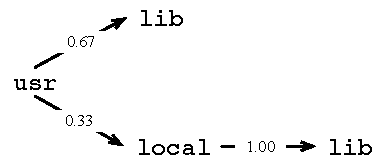
\includegraphics[scale=.7]{figures/host/syscall/probabilistic_tree}
  \caption{Probabilistic tree example.}
  \label{fig:albero}
\end{figure}

\paragraph{Discrete numeric values}
Flags, opening modes, etc. are usually chosen from a limited
set. Therefore we can store all of them along with a discrete
probability. Since in this case two values can only be ``equal'' or
``different'', we set up a binary distance model for clustering.

\begin{definition}[Discrete numeric args. distance]
  Let $x = i_{disc}$, $y = j_{disc}$ be the values of the arguments of
  type \emph{disc} (i.e., discrete numeric argument) of two instances
  $i$ and $j$ of the same system call. The \emph{distance} is defined
  as:

  \begin{displaymath}
    d_{disc}(i,j) := \left\{
      \begin{array}{lll}
        K_{disc} & \mbox{if $x \neq y$}\\
        0 & \mbox{if $x = y$},
    \end{array}
  \right.
\end{displaymath}

where $K_{disc}$ is a configuration parameter.
\end{definition}

Models fusion and incorporation of new elements are straightforward,
as well as the generation of probability for a new input to belong to
the model.

\begin{note}[Configuration parameters]
  According to the experiments described in
  Section~\ref{host:syscall:result-analysis}, the best detection
  accuracy is achieved with the default value of $K_{disc} = 1$. This
  parameter influences the quality of the clustering and thus may need
  to be changed if some particular, pathological false positives need
  to be eliminated in a specific setting.
\end{note}

\paragraph{Execution argument}
We also noticed that execution argument (i.e. the arguments passed to
the \texttt{execve} system call) are difficult to model, but we found the
length to be an extremely effective indicator of similarity of
use. Therefore we set up a binary distance model.

\begin{definition}[Execution arguments distance]
  Let $x = i_{disc}$ and $y = j_{disc}$ be the string values of the
  arguments of type \emph{disc} (i.e., execution argument) of two
  instances $i$ and $j$ of the same system call. The \emph{distance}
  is defined as:

\begin{displaymath}
  d_{arg}(i,j) := \left\{
    \begin{array}{lll}
      K_{arg} & \mbox{if $|x| \neq |y|$}\\
      0 & \mbox{if $|x| = |y|$},
    \end{array}
  \right.
\end{displaymath}

where $K_{arg}$ is a configuration parameter and $|x|$ is the length
of string $x$.
\end{definition}

\begin{note}[Configuration parameters]
  According to the experiments described in
  Section~\ref{host:syscall:result-analysis}, the best detection
  accuracy is achieved with the default value of $K_{arg} = 1$. This
  parameter influences the quality of the clustering and thus may need
  to be changed if some particular, pathological false positives need
  to be eliminated in a specific setting.
\end{note}

In this way, arguments with the same length are clustered
together. For each cluster, we compute the minimum and maximum value
of the length of arguments. Fusion of models and incorporation of new
elements are straightforward. The probability for a new input to
belong to the model is 1 if its length belongs to the interval, and 0
otherwise.

\paragraph{Token arguments}
Many arguments express \texttt{UID}s or \texttt{GID}s, so we developed
an ad-hoc model for \emph{users and groups} identifiers. Our reasoning
is that all these discrete values have three different meanings:
\texttt{UID} 0 is reserved to the super-user, low values usually are
for system special users, while real users have \texttt{UID}s and
\texttt{GID}s above a threshold (usually 1000). So, we divided the
input space in these three groups, and computed the distance for
clustering using the following definition.

\begin{definition}[UID/GID argument distance]
  Let $x = i_{disc}$ and $y = j_{disc}$ be the values of the arguments
  of type \emph{disc} (i.e., \texttt{GID}/\texttt{UID} argument) of
  two instances $i$ and $j$ of the same system call.

\begin{displaymath}
  d_{uid}(i,j) := \left\{
    \begin{array}{lll}
      K_{uid} & \mbox{if $g(x) = g(y)$}\\
      0 & \mbox{if $g(x) \neq g(y)$}
    \end{array}
  \right.,
\end{displaymath}

where $K_{uid}$ is a configuration parameter, the function $g:
\mathbb{N} \mapsto \{groups\}$ and $\{groups\}$ is the set of user
groups.
\end{definition}

Since \texttt{UID}s are limited in number, they are preserved for
testing, without associating a discrete probability to them. Fusion of
models and incorporation of new elements are straightforward. The
probability for a new input to belong to the model is 1 if the UID
belongs to the learned set, and 0 otherwise.

\begin{note}[Configuration parameters]
  According to the experiments described in
  Section~\ref{host:syscall:result-analysis}, the best detection
  accuracy is achieved with the default value of $K_{uid} = 1$. This
  parameter influences the quality of the clustering and thus may need
  to be changed if some particular, pathological false positives need
  to be eliminated in a specific setting.
\end{note}


\begin{table}[p]
  \centering
    \begin{tabular}{rll}
      \toprule
      \textsc{System call} & \multicolumn{2}{c}{\textsc{Model used for the arguments}} \\
      \midrule
      \texttt{open} & \texttt{pathname} & Path\\
      & \texttt{flags} & Discrete Numeric \\
      & \texttt{mode} & Discrete Numeric \\

      \texttt{execve} & \texttt{filename} & Path\\
      & \texttt{argv} & Execution Argument \\ 

      \texttt{setuid} & \texttt{uid} & User/Group\\
      \texttt{setgid} & \texttt{gid} & User/Group\\

      \texttt{setreuid} & \texttt{ruid} & User/Group\\
      \texttt{setregid} & \texttt{euid} & User/Group\\

      \texttt{setresuid, setresgid} & \texttt{ruid} & User/Group\\
      & \texttt{euid} & User/Group\\
      & \texttt{suid} & User/Group\\

      \texttt{symlink, link} & \texttt{oldpath} & Path\\
      \texttt{rename}& \texttt{newpath} & Path\\

      \texttt{mount} & \texttt{source} & Path\\
      & \texttt{target} & Path\\
      & \texttt{flags} & Discrete Numeric\\

      \texttt{umount} & \texttt{target} & Path\\
      & \texttt{flags} & Path\\

      \texttt{exit} & \texttt{status} & Discrete Numeric\\

      \texttt{chown} & \texttt{path} & Path\\
      \texttt{lchown} & \texttt{group} & User/Group\\
      & \texttt{owner} & User/Group\\

      \texttt{chmod, mkdir} & \texttt{path} & Path\\
      \texttt{creat} & \texttt{mode} & Discrete Numeric\\

      \texttt{mknode} & \texttt{pathname} & Path\\
      & \texttt{mode} & Discrete Numeric\\
      & \texttt{dev} & Discrete Numeric\\

      \texttt{unlink, rmdir} & \texttt{pathname} & Path\\
      \bottomrule
    \end{tabular}
    \caption{Association of models to system call arguments in our prototype}
  \label{tab:models-our-proto}
\end{table}

In Table \ref{tab:models-our-proto} we summarize the association of
the models described above with the arguments of each of the system
calls we take into account. This model based clustering is somehow
error prone since we would expect obtained centroids to be more
general and thus somehow to interfere when clustering either new or
old instances. To double check this possible issue we follow a simple
process:

\begin{enumerate}
\item creation of clusters on the training dataset;
\item generation of models from each cluster;
\item use of models to classify the original dataset into clusters,
  and check that inputs are correctly assigned to the same cluster
  they contributed to create.
\end{enumerate}

This is done both for checking the representativeness of the models,
and to double-check that the different distances computed make sense
and separate between different clusters.

\begin{table}[t]
  \centering
    \begin{tabular}{lccc}
      \toprule
      \textsc{Executable} & \textsc{\#elements} & \textsc{\% correct} & \textsc{Conf.}\\
      \midrule
      \texttt{fdformat} & 10 & 100\% & 1\\
      \texttt{eject} & 12 & 100\% & 1\\
      \texttt{ps} & 525 & 100\% & 1\\
      \texttt{telnetd} & 38 & 100\% & 0.954\\
      \texttt{ftpd} & 69 & 97.1\% & 0.675\\
      \texttt{sendmail} & 3211 & 100\% & 0.996\\
      \bottomrule
    \end{tabular}
  \caption{Cluster validation process.}
  \label{tab:cluster-validation}
\end{table}

As Table \ref{tab:cluster-validation} shows, for each program in the
\ac{IDEVAL}\index{IDEVAL} dataset (considering the representative open
system call), the percentage of inputs correctly classified, and a
confidence value, computed as the average ``probability to belong''
computed for each element w.r.t. the cluster it helped to build. The
results are almost perfect, as expected, with a lower value for the
ftpd program, which has a wider variability in file names.

\subsection{Capturing process behavior}
\label{host:syscall:markov}
To take into account the execution context of each system call, we use
a first order Markov chain to represent the program flow. The model
states represent the system calls, or better they represent the
various clusters of each system call, as detected during the
clustering process. For instance, if we detected three clusters in the
\texttt{open} system call, and two in the \texttt{execve} system call, then
the model will be constituted by five states: $\texttt{open}_1$,
$\texttt{open}_2$, $\texttt{open}_3$, $\texttt{execve}_1$,
$\texttt{execve}_2$. Each transition will reflect the probability of
passing from one of these groups to another through the program. As we
already observed in Section~\ref{detection:ad:host}, this approach was
investigated in former literature, but never in conjunction with the
handling of parameters and with a clustering approach.

A time domain process demonstrates a Markov property if the
conditional probability density of the current event, given all
present and past events, depends only on the $K$ most recent
events. $K$ is known as the \emph{order} of the underlying
model. Usually, models of order $K=1$ are considered, because they are
simpler to analyze mathematically. Higher-order models can usually be
approximated with first order models, but approaches for using
high-order Markov models in an efficient manner have also been
proposed, even in the intrusion detection field \citep{high}. A good
estimate of the order can be extracted from data using the criteria
defined in \citep{merhav}; for normal Markov models, a $\chi^2$-test
for first against second order dependency can be used
\citep{chiquadro}, but also an information criterion such as
\ac{BIC}\index{BIC} or \ac{MDL}\index{MDL} can be used.

\subsubsection{Training Phase}
Each execution of the program in the training set is considered as a
sequence of observations. Using the output of the clustering process,
each system call is classified into the correct cluster, by computing the
probability value for each model and choosing the cluster whose models
give out the maximum composite probability along all known models:
$\max(\prod_{i \in \mathrm{M}}{P_i})$. The probabilities of the Markov
model are then straightforward to compute. The final results can be
similar to what is shown in \ref{fig:markov}. On a first sight, this
could resemble a simple Markov chain, however it should be noticed
that each of the state of this Markov model could be mapped into the
set of possible cluster elements associated to it. From this
perspective, it could be seen as a very specific \ac{HMM}\index{HMM}
where states are fully observable through an uniform emission
probability over the associated syscalls\index{syscalls}. By simply turning the
clustering algorithm into one with overlapping clusters we could
obtain a proper \ac{HMM}\index{HMM} description of the user behavior
as it would be if we decide to further merge states together. This is
actually our ongoing work toward full \ac{HMM}\index{HMM} behavior
modeling with the aim, through overlapping syscalls\index{syscalls} clustering, of
improving the performance of the classical Baum-Welch algorithm and
solving the issue of \ac{HMM}\index{HMM} hidden space cardinality
selection~\citep{rabiner}. From our experiments, in the case of the
simple traces like the ones found in the \ac{IDEVAL}\index{IDEVAL}
dataset, the used model suffice so we are working on more complex
scenarios (i.e., new real datasets) to improve in a more grounded way
the proposed algorithm.

This type of model is resistant to the presence of a limited number of
outliers (e.g. abruptly terminated executions, or attacks) in the
training set, because the resulting transition probabilities will drop
near zero. For the same reason, it is also resistant to the presence
of any cluster of anomalous invocations created by the clustering
phase. Therefore, the presence of a minority of attacks in the
training set will not adversely affect the learning phase, which in
turn does not require then an attack-free training set.

The final result can be similar to what is shown in Figure
\ref{fig:markov}. In future extensions, the Markov model could then be
simplified by merging some states together: this would transform it in
a Hidden Markov Model, where the state does not correspond directly to
a system call cluster, but rather to a probability distribution of
possible outcomes. However, the use of \acp{HMM}\index{HMM}
complicates both training and detection phases \citep{rabiner}. From
our experiments, in the case of the simple traces like ones found in
the \ac{IDEVAL}\index{IDEVAL} dataset, this step is unnecessary.

\begin{figure}[t]
  \centering
  \begin{tikzpicture}[node distance=1.8cm,
    every node/.style={font=\footnotesize}]
    \node[state,initial]   (execve0)                         {ex$0$};
    \node[state]           (open24)  [right of=execve0]      {op$24$};
    \node[state]           (open12)  [right of=open24]       {op$12$};
    \node[state]           (open3)   [above right of=open12] {op$3$};
    \node[state]           (open45)  [right of=open12]       {op$45$};
    \node[state]           (rename0) [below right of=open12] {re$0$};
    \node[state]           (setuid0) [right of=rename0]      {se$0$};
    \node[state,accepting] (exit0)   [right of=open3]        {e$0$};

    \path[-stealth] (execve0) edge node [above] {1}    (open24)
                    (open24)  edge node [above] {1}    (open12)
                    (open12)  edge node [above left] {0.33} (open3)
                    (open12)  edge node [above] {0.33} (open45)
                    (open12)  edge node [below left] {0.33} (rename0)
                    (rename0) edge node [above] {1}    (setuid0)
                    (open45)  edge node [above] {1}    (setuid0)
                    (open3)   edge node [above] {0.50} (exit0)
                    (setuid0) edge node [right] {1}    (exit0)
                    (open3)   edge [loop above] node {0.50} ();
  \end{tikzpicture}
  \caption{Example of Markov model.}
  \label{fig:markov}
\end{figure}

\subsubsection{Detection Phase}
For detection, three distinct probabilities can be computed for each executed system call: the probability of the \emph{execution} sequence inside the Markov model up to now, $P_s$; the probability of the \emph{system call} to belong to the best-matching cluster, $P_c$; the \emph{last transition} probability in the Markov model, $P_m$.

The latter two probabilities can be combined into a single ``punctual'' probability of the single system call, $P_p = P_c \cdot P_m$, keeping a separate value for the ``sequence'' probability $P_s$. In order to set appropriate threshold values, we use the training data, compute the lowest probability over all the dataset for that single program (both for the sequence probability and for the punctual probability), and set this (eventually modified by a tolerance value) as the anomaly threshold. The tolerance can be tuned to trade off \ac{DR} for \ac{FPR}.

During detection, each system call is considered in the context of the process. The cluster models are once again used to classify each system call into the correct cluster as explained above: therefore ($P_c = \max(\prod_{i \in \mathrm{M}}{P_i})$). $P_s$ and $P_m$ are computed from the Markov model, and require our system to keep track of the current state for each running process. If either $P_s$ or $P_p = P_c \cdot P_m$ are lower than the anomaly threshold, the process is flagged as malicious.  

\begin{note}[Probability Scaling]
Given an $l$-long sequence of system calls, its sequence probability is $P_{s}(l) = \prod_{i = 0}^{l} P_{p}(i)$ where $P_{p}(i) \in [0,1]$ is the punctual probability of the $i$-th system call in the sequence. Therefore, it is self-evident that $\lim_{l \to +\infty} P_{s}(l) = 0$. Experimentally, we observed that the sequence probability quickly decreases to zero, even for short sequences (on the \ac{IDEVAL}\index{IDEVAL} dataset, we found that $P_{s}(l) \simeq 0$ for $l \geq 25$). This leads to a high number of false positives, since many sequences are assigned probabilities close to zero (thus, always lower than any threshold value).

To overcome this shortcoming, we implemented two probability scaling functions, both based on the geometric mean. As a first attempt, we computed $P_{s}(l) = \sqrt[l]{\prod_{i = 1}^{l} P_{p}(i)}$, but in this case

\begin{displaymath}
  \mathrm{P}\left[\lim_{l \to +\infty} P_{s}(l) = e^{-1}\right] = 1.
\end{displaymath}

\begin{proof}
  Let $\mathrm{G}(P_{p}(1), \ldots, P_{p}(l)) = \sqrt[l]{\prod_{i = 1}^{l} P_{p}(i)}$ the geometric mean of the sample $P_{p}(1), \ldots, P_{p}(l)$. If we assume that the sample is generated by a uniform distribution (i.e., $P_{p}(1), \ldots, P_{p}(l) \sim \mathcal{U}(0,1)$) then $\log P_{p}(i) \sim \mathcal{E}(\beta = 1) \: \forall i = 1, \ldots, l$: this can be proven by observing that the \ac{CDF} \citep{pestman} of $\log X$ (with $X = P_{p} \sim \mathcal{U}(0,1)$) equals the \ac{CDF}\index{CDF} of an exponentially distributed variable with $\beta = 1$.

  The arithmetic mean $\mathrm{A}(\cdot)$ of the sample

  \begin{displaymath}
    -\log(P_{p}(1)), \ldots, -\log(P_{p}(l))
  \end{displaymath}

  converges (in probability) to $\beta = 1$ for $l \to +\infty$, that is:
  \[
  \mathrm{P}\left[\lim_{l \to +\infty} \frac{1}{l}\sum_{i = 1}^{l} -\log P_{p}(i) = -\beta = -1 \right] = 1
  \]

  because of the strong law of large numbers. Being the geometric mean:

  \[
  \mathrm{G}(P_{p}(1), \ldots, P_{p}(l)) = \left(\prod_{i=1}^{l} P_{p}(i)\right)^{\frac{1}{l}} = e^{\frac{1}{l}\sum_{i = 1}^{l} -\log P_{p}(i)}
  \]

  we have

  \[
  \mathrm{P}\left[\lim_{l \to +\infty} \left( e^{\frac{1}{l}\sum_{i = 1}^{l} -\log P_{p}(i)} \right) = e^{-\beta} = e^{-1} \right] = 1
  \]
  \hfill$\qed$
\end{proof}

This is not our desired result, so we modified this formula to introduce a sort of ``forgetting factor'': $P_{s}(l) = \sqrt[2l]{\prod_{i = 1}^{l} P_{p}(i)^{i}}$. In this case, we can prove that $\mathrm{P}\left[\lim_{l \to +\infty} P_{s}(l) = 0\right] = 1$.

\begin{proof}
  The convergence of $P_{s}(l)$ to zero can be proven by observing that:
  \begin{eqnarray*}
    P_{s}(l) & = & \left(\sqrt[l]{\prod_{i = 1}^{l} P_{p}(i)^{i}}\right)^{\frac{1}{2}} = \left(e^{ \frac{1}{l} \sum_{i = 1}^{l} i \cdot \log P_{p}(i) }\right)^{\frac{1}{2}} =\\
    & = & \left(e^{ \frac{1}{l} \sum_{j = 0}^{l} \left( \sum_{i = 1}^{l-j} \log P_{p}(i) \right)}\right)^{\frac{1}{2}} =\\
    & = & \left(e^{ \sum_{j = 0}^{l} \left( \frac{1}{l} \sum_{i = 1}^{l} \log P_{p}(i) - \frac{1}{l} \sum_{i = l-j+1}^{l} \log P_{p}(i) \right)}\right)^{\frac{1}{2}}
  \end{eqnarray*}
  Because of the previous proof, we can write that:
  \[
  \mathrm{P}\left[\lim_{l \to +\infty} \frac{1}{l} \sum_{i = 1}^{l} \log P_{p}(i) = - 1 \right] = 1
  \]
  We can further observe that, being $\log P_{p}(i) < 0$:
  \[
  \forall j, l > 0: \sum_{i = 1}^{l} \log P_{p}(i) < \sum_{i = l-j+1}^{l} \log P_{p}(i)
  \]
  therefore, the exponent is a sum of infinite negative quantities lesser than $0$, leading us to the result that, \emph{in probability}
  \begin{eqnarray*}
    &&\lim_{l \to +\infty} \left(e^{ \sum_{j = 0}^{l} \left( \frac{1}{l} \sum_{i = 1}^{l} \log P_{p}(i) - \frac{1}{l} \sum_{i = l-j+1}^{l} \log P_{p}(i) \right) }\right)^{\frac{1}{2}} =\\
    &&\lim_{x \to -\infty} e^{x} = 0
  \end{eqnarray*}
  \hfill$\qed$
\end{proof}

Even if this second variant once again makes $P_{s}(l) \to 0$ (in probability), our experiments have shown that this effect is much \emph{slower} than in the original formula: $P_{s}(l) \simeq 0$ for $l \geq 300$ (vs. $l \geq 25$ of the previous version), as shown in Figure \ref{fig:normalization}. In fact, this scaling function also leads to much better results in terms of \ac{FPR} (see Section~\ref{host:syscall:result-analysis}).  
\end{note}

\begin{figure}[t]
  \centering
  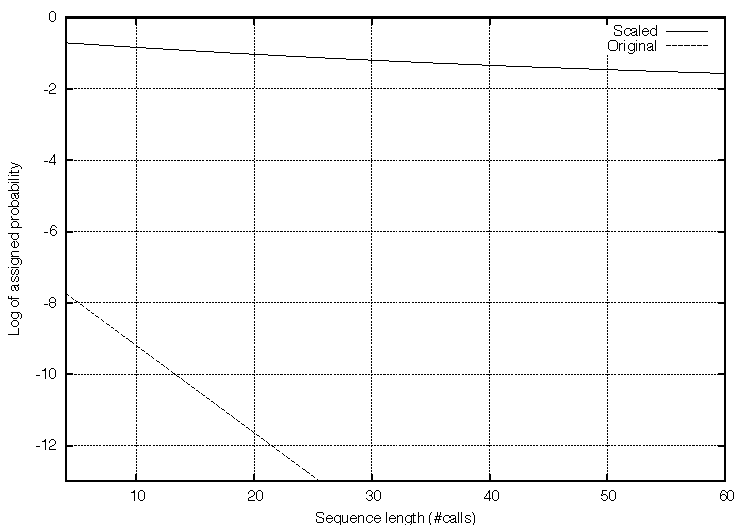
\includegraphics[width=.8\textwidth]{figures/host/syscall/normalization}
  \caption{Measured sequence probability (log) vs. sequence length, comparing the original calculation and the second variant of scaling.}
  \label{fig:normalization}
\end{figure}

Instead of using probabilities --- that are sensitive to the sequence length --- a possible alternative, which we are currently exploring, is the exploitation of distance metrics between Markov models \citep{stolcke93hidden,stolcke:icsi1994:merging,InducingProbabilisticGrammarsMerging} to define robust criteria to compare new and learned sequence models. Basically, the idea is to create and continuously update a Markov model associated to the program instance being monitored, and to check how much such a model differs from the ones the system has learned for the same program. This approach is complementary to the one proposed above, since it requires long sequences to get a proper Markov model. So, the use of both criteria (sequence likelihood in short activations, and model comparison in longer ones) could lead to a reduction of false positives on the sequence model.

\subsection{Prototype implementation}
\label{host:syscall:prot-impl}
We implemented the above described system into a two-stage, highly configurable, modular architecture written in \ac{ANSI}\index{ANSI} C. The high-level structure is depicted in Figure \ref{fig:architetura_hids}: the system is plugged into the Linux \texttt{auditd}. The Cluster Manager is in charge of the clustering phase while the Markov Model Manager implements Markov modeling features. Both the modules are used in both training phase and detection phase, as detailed below.

The Cluster Manager module implements abstract clustering procedures along with abstract representation and storage of generated clusters. The Markov Model Manager is conceptually similar to Cluster Manager: it has a basic Markov chains implementation, along with ancillary modules for model handling and storage.

During training, Cluster Manager is invoked to create the clusters on a given system call trail while Markov Model Manager infers the Markov model according to the clustering. At running time, for each system call, the Cluster Manager is invoked to find the appropriate cluster; the Markov Model Manager is also used to keep track of the current behavior of the monitored process: if significant deviations are found alerts are fired and logged accordingly.

The system can output to both standard output, \texttt{syslog} facilities and \ac{IDMEF}\index{IDMEF} files. Both the clustering phase and the behavioral analysis are multi-threaded and intermediate results of both procedures can be dumped in \ac{XML}\index{XML}.

\begin{figure}[t]
  \hspace*{-.9cm}
  \begin{tikzpicture}[node distance=6.5em,
    every node/.style={text centered,shape=rectangle,draw=black,font=\scriptsize},
    function/.style={font=\scriptsize\itshape,shape=rectangle,draw=black,dashed,thick},
    e/.style={text width=5em,font=\tiny\itshape,draw=none}
    ]

    \node (auditd) {\texttt{auditd}};
    \node [font=\tiny,text width=6em,draw=none,right of=auditd] (syscalls)
    {
      \texttt{execve(args**)}\\
      \texttt{<syscall>(args**)}\\
      \texttt{...}\\
      \texttt{exit()}
    };
    \node (clustering) [text width=3.8em,right of=syscalls] {Cluster Manager};
    \node (mm) [text width=3.8em,right of=clustering] {Markov Model Manager};
    \node (syslogd) at ($ (mm) + (5em,1em) $) {\texttt{syslogd}};
    \node [font=\tiny] (idmef) at ($ (mm) - (-5em,1em) $) {\texttt{<IDMEF />}};

    \node [e] at ($ (auditd) + (0,3em) $) {Kernel\\ Auditing};
    \node [e] at ($ (syscalls) + (0,3em) $) {Syscall \\ Extraction};
    \node [e] at ($ (clustering) + (0,3em) $) {Syscall\\ Classification};
    \node [e] at ($ (mm) + (0,3em) $) {Behavior\\ Modeling};
    \node [e] at ($ (syslogd) + (0,2em) $) {Alerting};

    \draw[-stealth] (auditd) to (syscalls);
    \draw[-stealth] (syscalls) to (clustering);
    \draw[-stealth] (clustering) to (mm);
    \draw[-stealth] (mm) to (syslogd);
    \draw[-stealth] (mm) to (idmef);
  \end{tikzpicture}
  \caption{The high-level structure of our prototype.}
  \label{fig:architetura_hids}
\end{figure}

\subsection{Experimental Results}
\label{host:syscall:result-analysis}
In this section, we both compare the detection accuracy of our
proposal and analyze the performances of the running prototype we
developed. Because of the known issues of \ac{IDEVAL}\index{IDEVAL}
(plus our findings summarized in
Section~\ref{detection:evaluation:darpa}), we also collected fresh
training data and new attacks to further prove that our proposal is
promising in terms of accuracy.

As we detailed in Section~\ref{host:syscall:clust-syst-calls}, our
system can be tuned to avoid overfitting\index{overfitting}; in the current
implementation, such parameters can be specified for \emph{each}
system call, thus in the following we report the bounds of variations
instead of listing \emph{all} the single values: $d_{stop,num} \in
\{1,2,3\}$, $d_{stop,min} = \{6,10,20,60\}$.

\subsubsection{Detection accuracy}
\label{host:syscall:detection-accuracy}
For the reasons outlined above and in
Section~\ref{detection:evaluation:darpa}, as well for the uncertainty
outlined in Section~\ref{host:syscall:crit-libanomaly}, we did not
rely on purely numerical results on \ac{DR} or \ac{FPR}. Instead, we
compared the results obtained by our software with the results of
\SyscallAnomaly in the terms of a set of case studies, comparing them
singularly. What turned out is that our software has two main
advantages over \LibAnomaly:

\begin{itemize}
\item a better contextualization of anomalies, which lets the system
  detect whether a single syscall has been altered, or if a sequence
  of calls became anomalous consequently to a suspicious attack;
\item a strong characterization of subgroups with closer and more
  reliable sub-models.
\end{itemize}

\begin{table}[p]
  \centering
  \begin{tabular}{rl}
    \toprule
    \textsc{HMM State} & \texttt{execve0} (\texttt{START} $\Rightarrow$ \texttt{execve0}) \\
    \cmidrule{2-2}
    filename & \texttt{/usr/bin/fdformat}\\
    argv & \texttt{fdformat$\backslash$0x20$\backslash$0x20$\backslash$0x20$\backslash$0x20[...]} \\
    \cmidrule{2-2}
    $P_c$ & $0.1$ \\
    $P_m$ & $1$ \\
    $P_p$ (thresh.) & $0.1$ ($1$)\\
    \midrule

    \textsc{HMM State} & \texttt{open10} (\texttt{open2} $\Rightarrow$ \texttt{open10}) \\
    \cmidrule{2-2}
    pathname & \texttt{/usr/lib/locale/iso\_8859\_1/[...]}\\
    flags & \texttt{-r-xr-xr-x} \\
    mode & \texttt{33133}\\
    \cmidrule{2-2}
    $P_c$ & $5 \cdot 10^{-4}$ \\
    $P_m$ & $0$ \\
    $P_p$ (thresh.) & $0$ (\emph{undefined})\\
    \midrule

    \textsc{HMM State} & \texttt{open11} (\texttt{open10} $\Rightarrow$ \texttt{open11}) \\
    \cmidrule{2-2}
    pathname & \texttt{/devices/pseudo/vol@0:volctl}\\
    flags & \texttt{crw-rw-rw-} \\
    mode & \texttt{8630}\\
    \cmidrule{2-2}
    $P_c$ & $1$ \\
    $P_m$ & $0$ \\
    $P_p$ (thresh.) & $0$ (\emph{undefined})\\
    \midrule

    \textsc{HMM State} & \texttt{chmod} (\texttt{open11} $\Rightarrow$ \texttt{chmod}) \\
    \cmidrule{2-2}
    pathname & \texttt{/devices/pseudo/vol@0:volctl}\\
    flags & \texttt{crw-rw-rw-} \\
    mode & \texttt{8630}\\
    \cmidrule{2-2}
    $P_c$ & $0.1$\\
    $P_m$ & $0$ \\
    $P_p$ (thresh.) & $0$ (\emph{undefined})\\
    \midrule

    \textsc{HMM State} & \texttt{exit0} (\texttt{chmod} $\Rightarrow$ \texttt{exit0}) \\
    \cmidrule{2-2}
    status & \texttt{0}\\
    \cmidrule{2-2}
    $P_c$ & $1$ \\
    $P_m$ & $0$ \\
    $P_p$ (thresh.) & $0$ (\emph{undefined})\\
    \bottomrule
  \end{tabular}
  \caption{\texttt{fdformat}: attack and consequences}
  \label{tab:fdformat-our-results}
\end{table}

As an example of the first advantage, let us analyze again the program
\texttt{fdformat}, which was already analyzed in
Section~\ref{host:syscall:crit-libanomaly}. As can be seen from Table
\ref{tab:fdformat-our-results}, our system correctly flags
\texttt{execve} as anomalous (due to an excessive length of input). It
can be seen that $P_m$ is 1 (the system call is the one we expected),
but the models of the syscall are not matching, generating a very low
$P_c$. The localization file opening is also flagged as anomalous for
two reasons: scarce affinity with the model (because of the strange
filename), and also erroneous transition between the open subgroups
\texttt{open2} and \texttt{open10}. In the case of such an anomalous
transition, thresholds are shown as ``undefined'' as this transition
has never been observed in training. The attack effect (\texttt{chmod}
and the change of permissions on \texttt{/export/home/elmoc/.cshrc})
and various intervening syscalls\index{syscalls} are also flagged as anomalous because
the transition has never been observed ($P_m = 0$); while reviewing
logs, this also helps us in understanding whether or not the buffer
overflow attack has succeeded. A similar observation can be done on
the execution of \texttt{chmod} on \texttt{/etc/shadow} ensuing an
attack on \texttt{eject}.

In the case of \texttt{ps}, our system flags the \texttt{execve}
system call, as usual, for excessive length of input. File
\texttt{/tmp/foo} is also detected as anomalous argument for
\texttt{open}. In \texttt{LibAnomaly}, this happened just because of
the presence of an underscore, and was easy to bypass. In our case,
\texttt{/tmp/foo} is compared against a sub-cluster of \texttt{open}
which contains only the \texttt{/tmp/ps\_data}, and therefore will
flag as anomalous, with a very high confidence, any other name, even
if structurally similar. A sequence of \texttt{chmod} syscalls\index{syscalls}
executed inside directory \texttt{/home/secret} as a result of the
attacks are also flagged as anomalous program flows.

\begin{table}[t]
  \centering
  \begin{tabular}{cccc}
    \toprule
    & \multicolumn{1}{c}{DR} & \multicolumn{2}{c}{FPR} \\
    \midrule
    \emph{Granularity:} & Sequence & Sequence & Call \\
    \midrule
    Markov model &\multicolumn{3}{c}{\texttt{bsdtar}}\\
    \cmidrule{2-4}
    Y & $100\%$ & $1.6\%$ & $0.1\%$ \\
    N & $88\%$ & $1.6\%$ & $0.1\%$ \\
    \midrule
    &\multicolumn{3}{c}{\texttt{eject}}\\
    \cmidrule{2-4}
    Y & $100\%$ & $0\%$ & $0\%$ \\
    N & $0\%$ & $0\%$ & $0\%$ \\
    \bottomrule
  \end{tabular}
  \caption{\acp{DR}\index{DR} and \acp{FPR}\index{FPR} on two test programs, with (Y) and without (N) Markov models.}
  \label{tab:res-sum}
\end{table}

Limiting the scope to the detection accuracy of our system, we
performed several experiments with both \texttt{eject} and
\texttt{bsdtar}\index{bsdtar}, and we summarize the results in Table
\ref{tab:res-sum}. The prototype has been trained with ten different
execution of \texttt{eject} and more than a hundred executions of
\texttt{bsdtar}\index{bsdtar}. We then audited eight instances of the activity of
\texttt{eject} under attack, while for \texttt{bsdtar}\index{bsdtar} we logged seven
malicious executions. We report \acp{DR}\index{DR} and
\acp{FPR}\index{FPR} with (Y) and without (N) the use of Markov
models, and we compute \acp{FPR}\index{FPR} using cross-validation
through the data set (i.e., by training the algorithm on a subset of
the dataset and subsequently testing the other part of the
dataset). Note that, to better analyze the false positives, we
accounted for both false positive sequences (Seq.) and false positive
system calls (Call).

In both cases, using the complete algorithm yield a 100\% \ac{DR} with
a very low \ac{FPR}. In the case of \texttt{eject}, the exploit is
detected in the very beginning: since a very long argument is passed
to the \texttt{execve}, this triggers the argument model. The
detection of the shellcode\index{shellcode} we injected exploiting the buffer overflow
in \texttt{bsdtar}\index{bsdtar} is identified by the \texttt{open} of the
unexpected (special) file \texttt{/dev/tty}. Note that, the use of
thresholds calculated on the overall Markov model allows us to achieve
a 100\% \ac{DR} in the case of \texttt{eject}; without the Markov
model, the attack wouldn't be detected at all.

\begin{figure}[t]
  \centering
  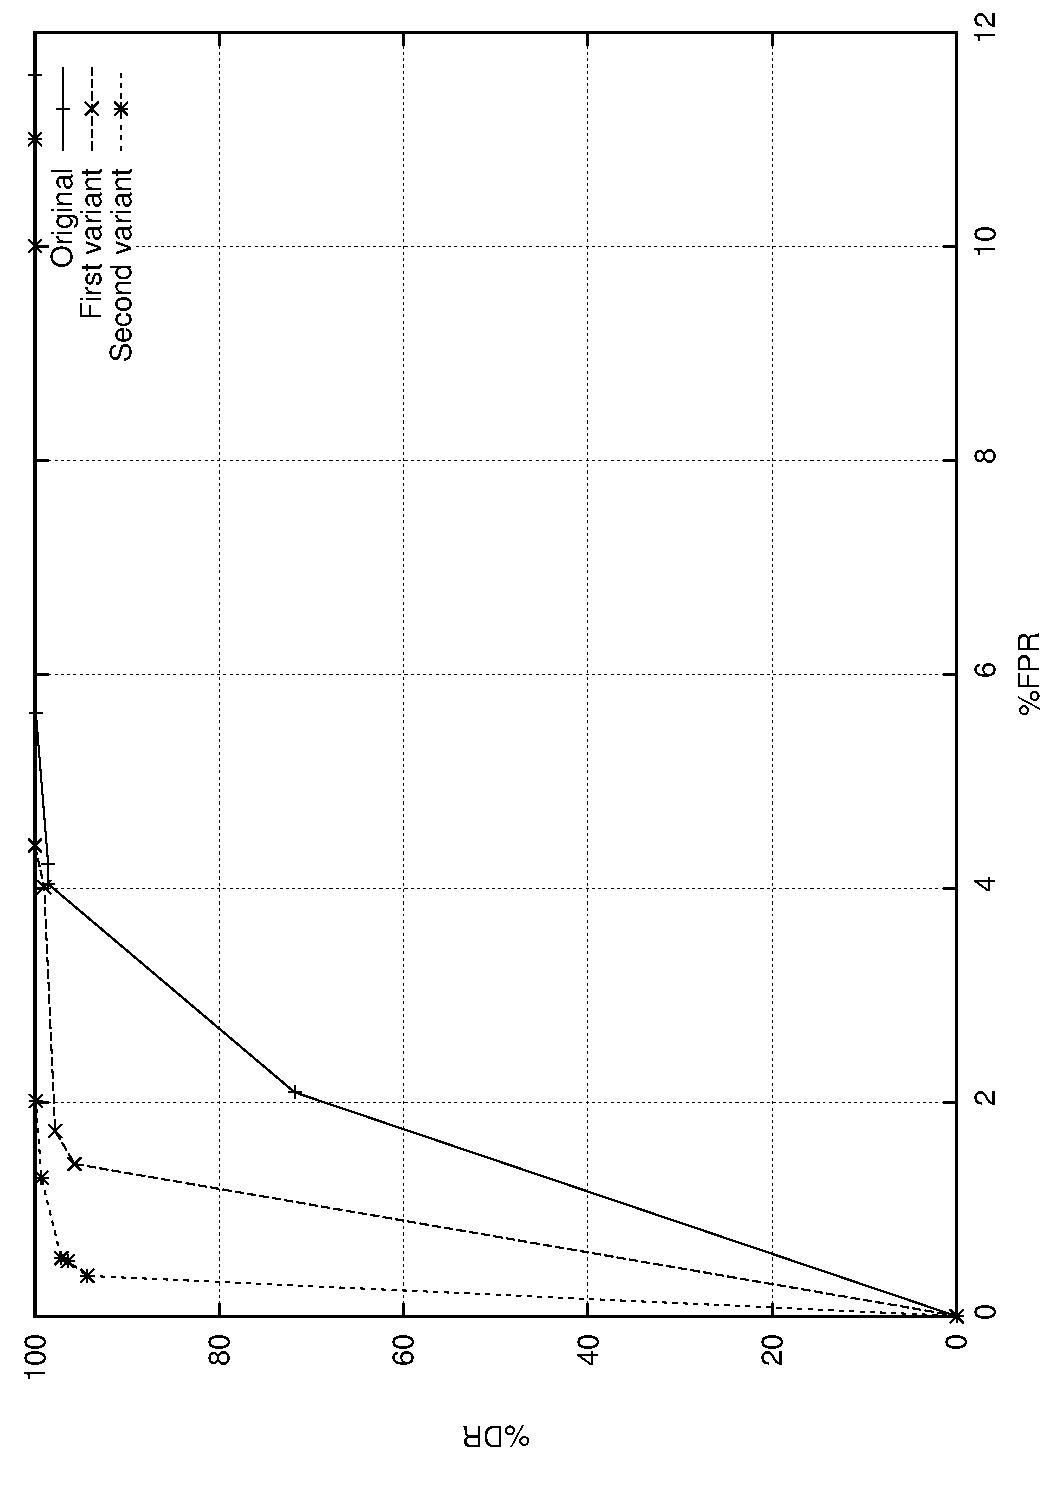
\includegraphics[angle=-90,width=\textwidth]{figures/host/syscall/roc}
  \caption{Comparison of the effect on detection of different probability scaling functions.}
  \label{fig:scaling_comparison}
\end{figure}

It is very difficult to compare our results directly with the other
similar systems we identified in Section~\ref{detection:ad:host}. In
\citep{rulessystemcallarguments} the evaluation is performed on the
\ac{DARPA}\index{DARPA} dataset, but \acp{DR}\index{DR} and
\acp{FPR}\index{FPR} are not given (the number of detections and false
alarms is not normalized), so a direct comparison is
difficult. Moreover, detection is computed using an arbitrary time
window, and false alerts are instead given in ``alerts per day''.  It
is correspondingly difficult to compare against the results in
\citep{venkat_dataflow}, as the evaluation is ran over a dataset which
is not disclosed, using two programs that are very different from the
ones we use, and using a handful of exploits chosen by the
authors. Different scalings of the false positives and
\acp{DR}\index{DR} also make a comparison impossible to draw.

As a side result, we tested the detection accuracy of the two scaling
functions we proposed for computing the sequence probability
$P_{s}$. As shown in Figure \ref{fig:scaling_comparison}, the first
and the second variant both show lower \ac{FPR} w.r.t. to the
original, unscaled version.

\begin{note}[Configuration parameters]
  Although we performed all the experiments with different values of
  $d_{stop,min}$ and $d_{stop,num}$, we report only the best detection
  accuracy, achieved with the default settings: $d_{stop,min} = 10$,
  $d_{stop,num} = 3$.

  These parameters influence the quality of the clustering and thus
  may need to be changed if some particular, pathological false
  positives need to be eliminated in a specific setting. In this case,
  human intervention is required; in particular, it is required to run
  the tool on a small dataset collected on a live system and check the
  clustering for outliers. If clusters containing too many outliers
  exist, then $d_{stop,min}$ may be increased. $d_{stop,num}$ should
  be increased only if outliers cannot be eliminated.
\end{note}

\subsubsection{Performance measurements}
\label{host:syscall:perf-meas}
An \ac{IDS}\index{IDS} should not introduce significant performance overheads in terms of the time required to classify events as malicious (or not). An \ac{IDS}\index{IDS} based on the analysis of system calls has to intercept and process every single syscall invoked on the operating system by userspace\index{userspace} applications; for this reason, the fastest a system call is processed, the best. We profiled the code of our system with \texttt{gprof} and \texttt{valgrind} for \ac{CPU}\index{CPU} and memory requirements. We ran the \ac{IDS}\index{IDS} on data drawn from the \ac{IDEVAL}\index{IDEVAL} 1999 dataset (which is sufficient for performance measurements, as in this case we are only interested in the throughput and not in realistic \acp{DR}\index{DR}).

In Table~\ref{tab:throughput} we reported the measurement of
performance on the five working days of the first week of the dataset
for training, and of the fourth week for testing. The throughput $X$
varies during training between 6120 and 10228 syscalls\index{syscalls}
per second. The clustering phase is the bottleneck in most cases,
while the Markov model construction is generally faster. Due to the
clustering step, the training phase is memory consuming: in the worst
case, we recorded a memory usage of about 700 MB. The performance
observed in the detection phase is of course even more important: in
this case, it varies between 12395 and 22266 syscalls/sec. Considering
that the kernel of a typical machine running services such as
\ac{HTTP}\index{HTTP}/F\ac{TP}\index{TP} on average executes system
calls in the order of thousands per second (e.g., around 2000 system
calls per second for \texttt{wu-ftpd} \citep{mutz06:syscalls}), the
overhead introduced by our \ac{IDS}\index{IDS} is noticeable but does
not severely impact system operations.

\begin{table}[p]
  \centering
  \begin{tabular}{lcccc}
    \toprule
    \multicolumn{5}{c}{\scshape Training throughput}\\
    \midrule
    Ses. & \#Calls & \#Progr. & $t$ (Clust., HMM) [$s$] & $X$ [$call/s$]\\
    \midrule
    1 & 97644 & 111 & 12.056 (7.683, 3.268) & 8099\\ 
    2 & 34931 & 67 & 3.415 (1.692, 1.356) & 10228\\ 
    3 & 41133 & 129 & 6.721 (3.579, 2.677) & 6120\\ 
    4 & 50239 & 152 & 7.198 (3.019, 3.578) & 6979\\ 
    5 & 38291 & 115 & 4.503 (2.219, 1.849) & 8503\\ 
    \midrule
    \multicolumn{3}{l}{Avg. processing time} & $1.2910 \cdot 10^{-4}$ &\\
    \midrule
    \multicolumn{5}{c}{\scshape Detection throughput}\\
    \midrule
    Ses. & \#Calls & \#Progr. & $t$ [$s$] & $X$ [$call/s$]\\
    \midrule
    1 & 109160 & 149 & 6.722 & 16239\\ 
    2 & 160565 & 186 & 12.953 & 12395\\ 
    3 & 103605 & 143 & 4.653 & 22266\\ 
    4 & 115334 & 107 & 5.212 & 22128\\ 
    5 & 112242 & 147 & 5.674 & 19781\\ 
    \midrule
    \multicolumn{3}{l}{Avg. processing time} & $5.6581 \cdot 10^{-5}$ &\\
  \end{tabular}
  
  \caption{Training and detection throughput $X$. On the same dataset,
    the average processing time with \SSAADE disabled is around
    $0.08741084$, thus, in the worst case, \SSAADE introduces a
    $0.1476\%$ overhead (estimated).}
  \label{tab:throughput}
\end{table}

\section{Mixing Deterministic and Stochastic Models}
\label{host:improving}
In this section, we describe an improvement to the syscall-based anomaly detection system described in Section \ref{host:syscall}, which incorporates both the deterministic models of what we called FSA-DF, detailed in \citep{venkat_dataflow} (that we analyzed in detail in Section \ref{detection:ad:host}), and the stochastic models of \ac{SSAADE}. In \citep{2009_frossi_maggi_rizzo_zanero_improving_syscall_models} we propose a number of modifications, described in the following, that significantly improve the performance of both the original approaches. In this section we begin by comparing FSA-DF with \ac{SSAADE} and analyzing their respective performance in terms of detection accuracy. Then, we outline the major shortcomings of the two systems, and propose various changes in the models that can address them. In particular, we kept the deterministic control flow model of FSA-DF and substituted some deterministic dataflow relations with their stochastic equivalent, using the technique described in Section~\ref{host:improving:path-model}. This allowed us to maintain an accurate characterization of the process control flow and, at the same time, to avoid many \ac{FP} due to the deterministic relations among arguments. More precisely, the original learning algorithm of FSA-DF can be schematized as follow:

\begin{pseudo}
  $\forall \mathtt{c} = \langle syscall_{i-1}, syscall_{i} \rangle$
  make_state(c, PC)
  learn_relations(c)
    equal
    elementOf
    subsetOf
    range
    hasExtension
    isWithinDir
    contains
    hasSameDirAs
    hasSameBaseAs
    hasSameExtensionAs
\end{pseudo}

We noticed that simple relations such as \textsf{equal}, \textsf{elementOf}, \textsf{contains} were not suitable for strings. In particular, they raise too many \ac{FP} also in obvious cases like \texttt{``/tmp/php1553''} \emph{vs.} \texttt{``/tmp/php9022''} where the deterministic \texttt{equal} does not hold, but a smoother predicate could easily detect the common prefix, and thus group the two strings in the same class. This problem is clearly extended to the other two relations that are based on string confrontation as well. To mitigate these side-effects, we augmented the learning algorithm as follows:

\begin{pseudo}
  learn_string_domain($\mathtt{syscall}_{i}$)
  $\forall \mathtt{c} = \langle \mathtt{syscall}_{i-1}, \mathtt{syscall}_{i} \rangle$
  make_state(c, PC)
  learn_relations(c)
    save_model
    subsetOf
    range
    hasExtension
    isWithinDir
    hasSameDirAs
    hasSameBaseAs
    hasSameExtensionAs
\end{pseudo}

where the pseudo-function \texttt{learn\_string\_domain} equals to the training of the \ac{SOM} as described in Section~\ref{host:improving:path-model}, and \texttt{save\_model} plays the role the three relations mentioned above. Basically, it stores the \ac{BMU} corresponding to the string arguments of the current system call. The \ac{BMU} is retrieved by querying the \ac{SOM} previously trained. In addition to this, we complemented the resulting system with two new models to cope with \ac{DoS} attacks (see Section~\ref{host:improving:dos-detection-using}) and the presence of outlier in the training dataset (see Section~\ref{host:improving:exec-models}).

We show how targeted modifications of their anomaly models, as opposed to the redesign of the global system, can noticeably improve the overall detection accuracy. Finally, the impact of these modifications are discussed by comparing the performance of the two original implementations with two modified versions complemented with our models.

\subsection{Enhanced Detection Models}
\label{host:improving:improved-models}
The improvements we made focus on \emph{path} and \emph{execution} arguments. A new \emph{string length} model is added exploiting a Gaussian interval as detailed in Section~\ref{host:improving:exec-models}. The new \emph{edge frequency} model described in Section~\ref{host:improving:dos-detection-using} have been added to detect \ac{DoS} attacks. Also, in Section~\ref{host:improving:path-model} we describe how we exploited \ac{SOM} to model the similarity among \emph{path arguments}. The resulting system, Hybrid IDS incorporates the models of FSA-DF and \ac{SSAADE} along with the aforementioned enhancements.

\subsubsection{Arguments Length Using Gaussian Intervals}
\label{host:improving:exec-models}
The model for system call execution arguments implemented in \ac{SSAADE} takes into account the minimum and maximum length of the parameters found during training, and checks whether each string parameter falls into this range (model probability 1) or not (model probability 0). This technique allows to detect common attempts of buffer overflow through the command line, for instance, as well as various other command line exploits. However, such criteria do not model ``how different'' two arguments are to each others; a smoother function is more desirable. Furthermore, the frequency of each argument in the training set is not taken into account at all. Last but not least, the model is not resilient to the presence of attacks in the training set; just one occurrence of a malicious string would increase the length of the maximum interval allowing argument of almost every length.

The improved version of the interval model uses a Gaussian distribution for modeling the argument length $X_{args} = |args|$, estimated from the data in terms of sample mean and sample variance. The anomaly threshold is a percentile $T_{args}$ centered on the mean. Arguments which length is \emph{outside} the stochastic interval are flagged as anomalous. This model is resilient to the presence of outliers in the dataset. The Gaussian distribution has been chosen since is the natural stochastic extension of a range interval for the length. An example is shown in Figure \ref{fig:args_distribution_normal}.

\begin{figure}[t]
  \hspace*{-0.3cm}
  \begin{tabular}{lr}
    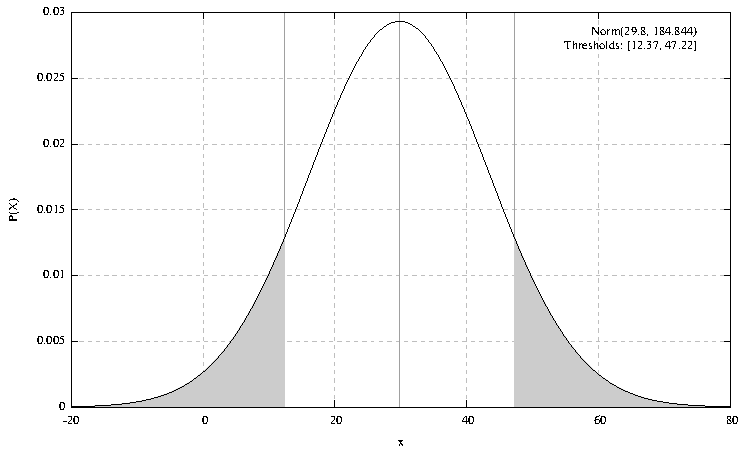
\includegraphics[width=.48\textwidth]{figures/host/improving/args_normal} &
    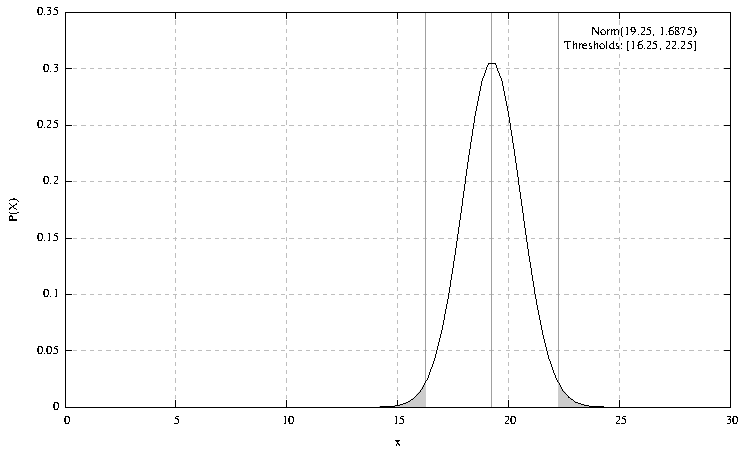
\includegraphics[width=.48\textwidth]{figures/host/improving/args_normal_1}
  \end{tabular}
  \caption[Sample estimated Gaussian intervals for string length.]{Sample estimated Gaussian intervals for string length. Training data of \texttt{sudo} (left) and \texttt{ftp} (right) was used. $\mathcal{N}(29.8, 184.844)$, thresholds [12.37, 47.22] (left) and $\mathcal{N}(19.25, 1.6875)$, thresholds [16.25, 22.25] (right).}
  \label{fig:args_distribution_normal}
\end{figure}

\paragraph{Model Validation} During detection the model self-assesses its precision by calculating the kurtosis measure \citep{joanes1998cms}, defined as $\gamma_{X} = \frac{\mathrm{E}^{4}(X)}{\mathrm{\mathrm{Var}(X)^{2}}}$. Thin tailed distributions with a low peak around the mean exhibit $\gamma_{X} < 0$ while positive values are typical of fat tailed distributions with an acute peak. We used $\hat{\gamma}_{X} = \frac{\mu_{X,4}}{\sigma^{4}_{X}} - 3$ to estimate $\gamma_{X}$. Thus, if $\gamma_{X_{args}} < 0$ means that the sample is spread on a big interval, while positive the values indicates a less ``fuzzy'' set of values. It is indeed straightforward that highly negative values indicates not significant estimations as the interval would include almost all lengths. In this case, the model falls back to a simple interval.

\subsubsection{DoS Detection Using Edge Traversal Frequency}
\label{host:improving:dos-detection-using}
\ac{DoS} attacks which force the process to get stuck in a legal section of the normal control flow could be detected by \ac{SSAADE} as violations of the Markov model, but not by FSA-DF. On the other hand, the statistical models implemented in \ac{SSAADE} are more robust but have higher \acp{FNR}\index{FNR} than the deterministic detection implemented in FSA-DF. However, as already stated in Section~\ref{host:syscall}, the cumulative probability of the traversed edges works well only with execution traces of similar and fixed length, otherwise even the rescaled score decreases to zero, generating false positives on long traces.

\begin{figure}[t]
  \hspace*{-0.3cm}
  \subfloat[][]{
    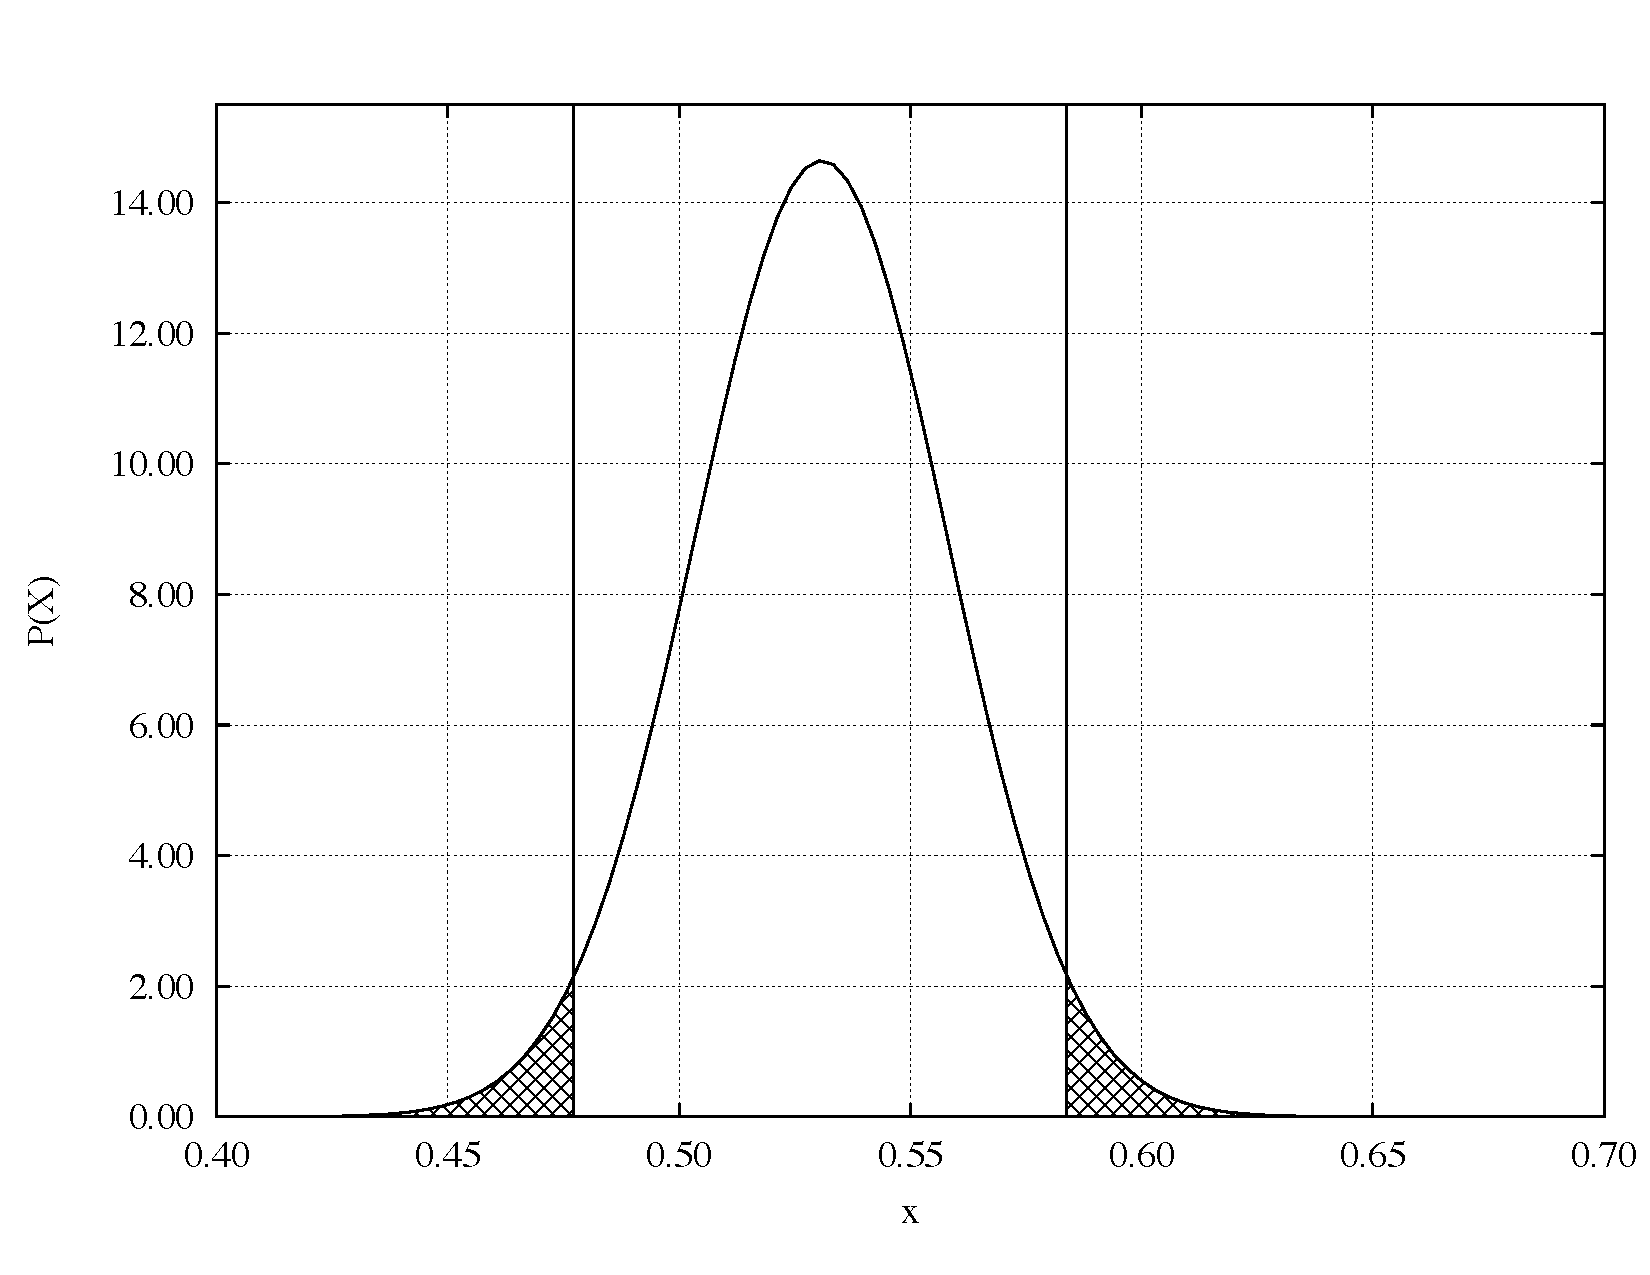
\includegraphics[width=.48\textwidth]{figures/host/improving/beta_left}
  }
  \subfloat[][]{
    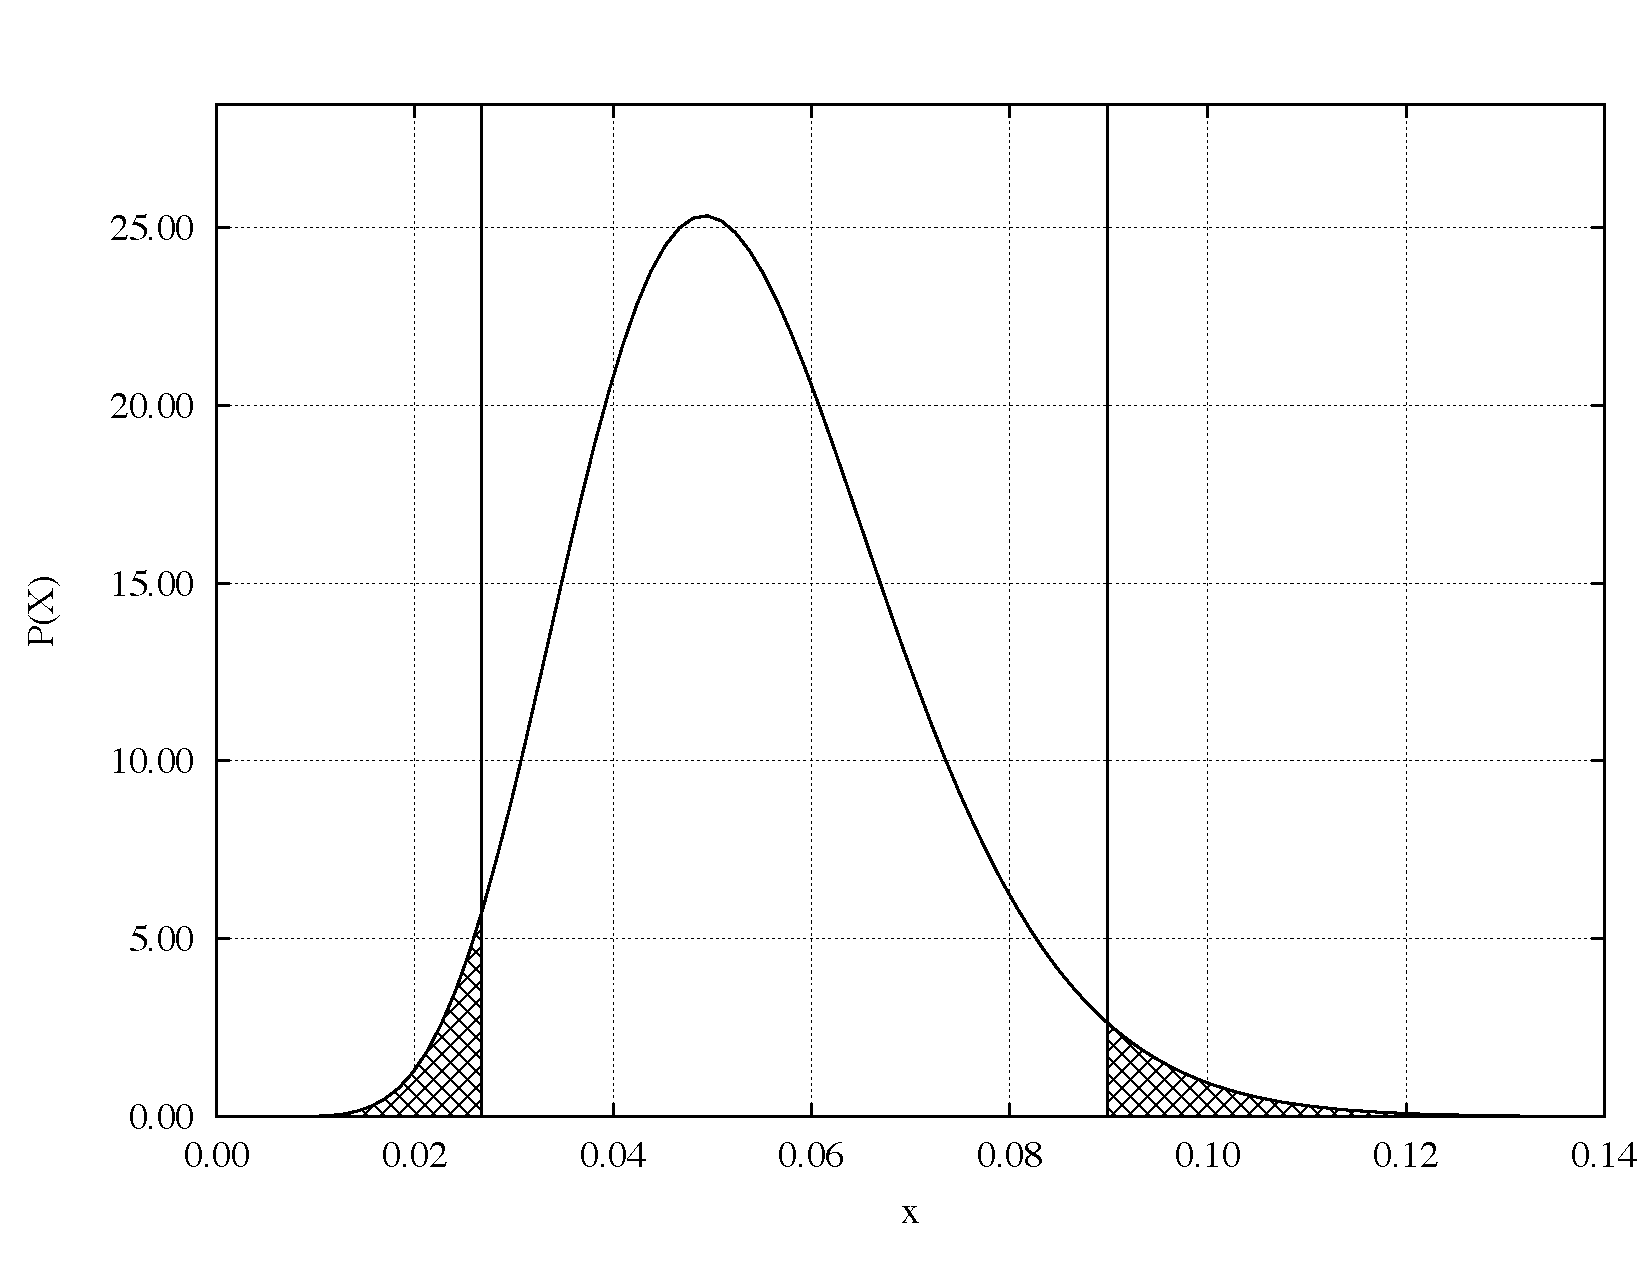
\includegraphics[width=.48\textwidth]{figures/host/improving/beta_right}
  }
  \caption{Two different estimations of the edge frequency distribution. Namely, Beta(178.445, 157.866) with thresholds [0.477199, 0.583649] (left) and Beta(10.3529,181.647) with thresholds [0.0266882, 0.0899057] (right).}
  \label{fig:execve beta}
\end{figure}

To solve these issues a stochastic model of the edge frequency traversal is used. For each trace of the training set, our algorithm counts the number of edge traversals (i.e., Markov model edge or \ac{FSA}\index{FSA} edge). The number is then normalized w.r.t. all the edges obtaining frequencies. Each edge is then associated to the sample $X_{edge} = x_{1}, x_{2}, \dots$. We show that the random samples $X_{edge}$ is well estimated using a Beta distribution. Figure \ref{fig:execve beta} shows sample plots of this model estimated using the \texttt{mt-daapd} training set; the quantiles associated to the thresholds are computed and shown as well. As we did for the Gaussian model, the detection thresholds are defined at configuration time as a percentile $T_{edge}$ centered on the mean (Figure \ref{fig:execve beta}). We chose the Beta for its high flexibility; a Gaussian is unsuitable to model skewed phenomena.

\paragraph{Model Validation} Our implementation is optimized to avoid
overfitting\index{overfitting} and meaningless estimations. A model is
valid only if the training set includes a significant (e.g.,
$|\min_{i}\{x_{i}\} - \max_{i}\{x_{i}\}| \geq \delta x_{min} = 0.04$)
amount ($N_{edge}^{min} = 6$) of paths. Otherwise it construct a
simpler frequency range model. The model exhibits the side effect of
discarding the extreme values found in training and leads to erroneous
decisions. More precisely, if the sample is $X_{edge} = 1, 1, \dots,
0.9, 1$, the right boundary will never be exactly $1$, and therefore
legal values will be discarded. To solve this issue, the quantiles
close to $1$ are approximated to $1$ according to a configuration
parameter $\bar{X}_{cut}$. For instance, if $\bar{X}_{cut} = 3$ the
quantile $F_{X}(\cdot) = 0.99\underline{\bar{9}}$ is approximated to
$1$.

\subsubsection{Path Similarity Using Self Organizing Maps}
\label{host:improving:path-model}
Path argument models are already implemented in \ac{SSAADE} and FSA-DF. Several, general-purpose string comparison techniques have been proposed so far, especially in the field of database systems and data cleansing \citep{elmagarmid2007drd}. We propose a solution based on Symbol-\acp{SOM}\index{SOM} \citep{symbolsom_online} to define an accurate distance metric between paths. Symbol \ac{SOM}\index{SOM} implements a smooth similarity measure otherwise unachievable using common, crisp distance functions among strings (e.g., edit distance).

The technique exploits \acp{SOM}\index{SOM}, which are unsupervised neural algorithms. A \ac{SOM} produces a compressed, multidimensional representation (usually a bi-dimensional \emph{map}) of the input space by preserving the main topological properties. It is initialized randomly, and then adapted via a competitive and cooperative learning process. At each cycle, a new input is compared to the known models, and the \ac{BMU} node is selected. The \ac{BMU} and its neighborhood models are then updated to make them better resemble future inputs.

We use the technique described in \citep{symbolsom_intro} to map \emph{strings} onto \acp{SOM}\index{SOM}. Formally, let

\begin{displaymath}
  S_{t} = [s_{t}(1)\cdots s_{t}(L)]
\end{displaymath}

denote the $t$-th string over the alphabet $\mathcal{A}$ of size $|\mathcal{A}|$. Each symbol $s_{t}(i), i = 1 \ldots L$, is then encoded into a vector $\underline{s}_{t}(i)$ of size $|\mathcal{A}|$ initialized with zeroes except at the $w$-th position which corresponds to the index of the encoded symbol (e.g., $s_{t}(i) = `b'$ would be $\underline{s}_{t}(i) = [0~1~0~0 \cdots 0]^{T}$, $w = 2$). Thus, each string $S_{t}$ is represented with sequence of $L$ vectors like $\underline{s}_{t}(i)$, i.e. a $L \times |\mathcal{A}|$-matrix: $\underline{\underline{S}}_{t}$.

Let $\underline{\underline{S}}_{t}$ and
$\underline{\underline{M}}_{k}$ denote two vector-encoded strings,
where $\underline{\underline{M}}_{k}$ is the model associated with
\ac{SOM}\index{SOM} node $k$. The distance between the two strings is
$D'(S_{t}, M_{k}) = D(\underline{\underline{S}}_{t},
\underline{\underline{M}}_{k})$. $D(\cdot, \cdot)$ is also defined in
the case of $L_{S_{t}} = |S_{t}| \neq |M_{k}| = L_{M_{k}}$ relying on
dynamic time warping techniques to find the best alignment between the
two sequences before computing the distance. Without going into
details, the algorithm \citep{symbolsom_online} aligns the two
sequences $\underline{s}_{t}(i) \in \underline{\underline{S}}_{t},
\underline{m}_{k}(j) \in \underline{\underline{M}}_{k}$ using a
mapping $[\underline{s}_{t}(i), \underline{m}_{k}(j)]$ $\mapsto$
$[\underline{s}_{t}(i(p)), \underline{m}_{k}(j(p))]$ defined through
the warping function $F: [i, j] \mapsto [i(p), j(p)]$:

\begin{displaymath}
  F = [[i(1), j(1)], \dots, [i(p), j(p)], \dots, [i(P), j(P)]].
\end{displaymath}

The distance function $D$ is defined over the warping alignment of size $P$, $D(\underline{\underline{S}}_{t}, \underline{\underline{M}}_{k}) = \sum_{p = 1}^{P} d(i,j)$, which is $P = L_{S_{t}} = L_{M_{k}}$ if the two strings have equal lengths. More precisely:

\begin{displaymath}
  d(i,j) = d(i(p), j(p)) ||\underline{s}_{t}(i(p)) - \underline{m}_{k}(j(p))||.
\end{displaymath}

The distance is defined upon $g_{i,j} = g(i, j)$, the variable which stores the cumulative distance in each trellis point $(i, j) = (i(p), i(p))$. The trellis is first initialized to $0$ in $(0,0)$, to $+\infty$ for both $(0,\cdot)$ and $(\cdot,0)$, otherwise:

\begin{displaymath}
  g(i,j) = \min\left\{
    \begin{array}{l}
      g(i,j-1) + d(i,j)\\
      g(i-1,j-1) + d(i,j)\\
      g(i-1,j) + d(i,j)
    \end{array}\right.
\end{displaymath}

Note that $i \in [1, L_{S_{t}}]$ and $j \in [1, L_{M_{k}}]$ thus the total distance is $D(\underline{\underline{S}}_{t}, \underline{\underline{M}}_{k}) = g(L_{S_{t}}, L_{M_{k}})$. A simple example of distance computation is show in Figure \ref{fig:distance-matrix} ($\mathcal{A}$ is the English alphabet plus extra characters). The overall distance is $D'(S_{t}, M_{k}) = 8.485$. We used a symmetric Gaussian neighborhood function $h$ whose center is located at the \ac{BMU}\index{BMU} $c(t)$. More precisely

\begin{displaymath}
  h(k, c(t), t) = \alpha(t) e^{-\frac{d(c(t),k)}{2\sigma^{2}(t)}}
\end{displaymath}


where $\alpha(t)$ controls the learning rate and $\sigma(t)$ is the actual width of the neighborhood function. The \ac{SOM}\index{SOM} algorithm uses \emph{two} training cycles. During (1) \emph{adaptation} the map is more flexible, while during (2) \emph{tuning} the learning rate $\alpha_{(\cdot)}$ and the width of the neighborhood $\sigma_{(\cdot)}$ are decreased. On each phase such parameters are denoted as $\alpha_{1}, \alpha_{2}, \sigma_{1}, \sigma_{2}$.

\begin{figure}[t]
  \begin{equation*}
     \bordermatrix{
      &&               \mathsf{/}&\mathsf{b}&\mathsf{i}&\mathsf{n}&\mathsf{/}&\mathsf{s}&\mathsf{h} \cr
      &0&+\infty&+\infty&+\infty&+\infty&+\infty&+\infty&+\infty \cr
      \mathsf{/}&+\infty & 0 &  1.414 & 2.828 & 4.242 & 4.242 & 5.656 & 7.071 \cr
      \mathsf{v}&+\infty & 1.414 & 1.414 & 2.828 & 4.242 & 5.656 & 5.656 & 7.071 \cr
      \mathsf{a}&+\infty & 2.828 & 2.828 & 2.828 & 4.242 & 5.656 & 7.071 & 7.071 \cr
      \mathsf{r}&+\infty & 4.242 & 5.656 & 5.656 & 5.656 & 4.242 & 5.656 & 7.071 \cr
      \mathsf{/}&+\infty & 4.242 & 4.242 & 4.242 & 4.242 & 5.656 & 7.071 & 8.485 \cr
      \mathsf{l}&+\infty & 5.656 & 5.656 & 7.071 & 7.071 & 5.656 & 5.656 & 7.071 \cr
      \mathsf{o}&+\infty & 7.071 & 7.071 & 7.071 & 8.485 & 7.071 & 7.071 & 7.071 \cr
      \mathsf{g}&+\infty & 8.485 & 8.485 & 8.485 & 8.485 & 8.485 & 8.485 & \mathbf{8.485}
    }
  \end{equation*}

  \caption{Distance computation example.}
\label{fig:distance-matrix}
\end{figure}

Symbol \acp{SOM}\index{SOM} are ``plugged'' into FSA-DF by associating each transition with the \emph{set} of \acp{BMU}\index{BMU} learned during training. At detection, an alert occurs whenever a path argument falls into neighborhood of a non-existing \ac{BMU}\index{BMU}. Similarly, in the case of \ac{SSAADE}, the neighborhood function is used to decide whether the string is anomalous or not, according to a proper threshold which is the minimum value of the neighborhood function encountered during training, for each node.

\subsection{Experimental Results}
\label{host:improving:accuracy}
In this section we describe our efforts to cope with the lack of reliable testing datasets for intrusion detections. The testing methodology is here detailed along with the experiments we designed. Both detection accuracy and performance overhead are subjects of our tests.

\begin{table}[p]
  \centering\footnotesize
  \begin{tabular*}{\columnwidth}{@{\extracolsep{\fill}}rccccccc}

    \toprule

    & \texttt{sing} & \texttt{mt-daapd} & \texttt{proftpd} & \texttt{sudo} & \multicolumn{1}{c}{\texttt{BitchX}}\\

    \midrule

    SOM & 15 $\times$ 15 & 15 $\times$ 15 & 15 $\times$ 15 & 15 $\times$ 15 & 10 $\times$ 10\\
    Traces & 18 & 18 & 18 & 18 & 14\\
    Syscalls & 5808 & 194879 & 64640 & 52034 & 103148\\
    Paths & 2700 & 2700 & 23632 & 1316 & 14921 \\
    Paths/cycle\% & 2 & 2 & 1 & 8 & 1 \\
    \bottomrule
  \end{tabular*}
  
  \caption{Parameters used to train the \acp{IDS}\index{IDS}. Values includes the number of traces used, the amount of paths encountered and the number of paths per cycle.}
  \label{tab:testing}
\end{table}

In order to evaluate and highlight the impact of each specific model, we performed targeted tests rather than reporting general \acp{DR}\index{DR} and \acp{FPR}\index{FPR} only. Also, we ensured that all possible alerts types are inspected (i.e., true/false positive/negative). In particular, for each \ac{IDS}\index{IDS}, we included one \emph{legal} trace in which file operations are performed on files \emph{never} seen during training but with a similar name (e.g., training on \texttt{/tmp/log}, testing on \texttt{/tmp/log2}); secondly, we inserted a trace which mimics an attack.

\subsubsection{Comparison of Detection Accuracy}
\label{host:improving:test_hybrid}
The detection accuracy of Hybrid IDS (H), FSA-DF (F) and \ac{SSAADE} (S) is here analyzed and compared. Both training parameters and detection results are summarized in Table \ref{tab:testing}. The parameters used to train the \ac{SOM}\index{SOM} are fixed except for $\sigma_{1}(t)$: $\alpha_{1}(t) = 0.5\div0.01$, $\sigma_{2}(t) = 3$ and $\alpha_{2}(t) = 0.1\div0.01$. Percentiles for both $X_{args}$ and $X_{edge}$ are detailed. The ``paths/cycle\%'' (paths per cycle) row indicates the amount of paths arguments used for training the \ac{SOM}\index{SOM}. The settings for clustering stage of \ac{SSAADE} are constant: minimum number of clusters ($3$, or $2$ in the case of the \texttt{open}); maximum merging distance ($6$, or $10$ in the case of the \texttt{open}); the ``null'' and the ``don't care'' probability values are fixed at $0.1$ and $10$, respectively, while $10$ is the maximum number of leaf clusters. In order to give a better understanding of how each prototype works, we analyzed by hand the detection results on each target application.

\begin{table}[p]
  \centering\footnotesize
  \begin{tabular*}{\columnwidth}{@{\extracolsep{\fill}}rccccccc}

    \toprule

       & \texttt{sing} & \texttt{mt-daapd} & \texttt{profdtpd} & \texttt{sudo} & \multicolumn{1}{c}{\texttt{BitchX}}\\

    \midrule

    Traces & 22 & 18 & 21 & 22 & 15\\
    Syscalls & 1528 & 9832 & 18114 & 3157 & 107784\\
    \ac{SSAADE} & 10.0\% & 0\% & 0\% & 10.0\% & 0.0\%\\
    FSA-DS & 5.0\% & 16.7\% & 28\% & 15.0\% & 0.0\%\\
    Hybrid IDS & 0.0\% & 0\% & 0\% & 10.0\% & 0.0\%\\

    \bottomrule
  \end{tabular*}
  
  \caption{Comparison of the \ac{FPR} of \ac{SSAADE} vs. FSA-DF vs. Hybrid IDS. Values include the number of traces used. Accurate description of the impact of each \emph{individual} model is in Section~\ref{host:improving:test_hybrid}}
  \label{tab:testing2}
\end{table}

\begin{description}
  \item [\texttt{sing}:] Hybrid IDS is not tricked by the false positive mimic trace inserted. The Symbol SOM model recognizes the similarity of \texttt{/tmp/log3} with the other paths inserted in the training. Instead, both FSA-DF and \ac{SSAADE} raise false alarms; the former has never seen the path during training while the latter recognizes the string in the tree path model but an alarm is raised because of threshold violation. \ac{SSAADE} recognizes the attack containing the longer subsequent invocations of \texttt{mmap2}; FSA-DF also raises a violation in the file name because it has never been trained against \texttt{/etc/passwd} nor \texttt{/etc/shadow}; and Hybrid IDS is triggered because the paths are placed in a different \ac{SOM}\index{SOM} region w.r.t. the training.
  \item[\texttt{mt-daapd}:] The legit traces violate the binary and unary relations causing several false alarms on FSA-DF. On the other hand, the smoother path similarity model allows Hybrid IDS and \ac{SSAADE} to pass the test with no false positives. The changes in the control flow caused by the attacks are recognized by all the \acp{IDS}\index{IDS}. In particular, the DoS attack (special-crafted request sent fifty times) triggers an anomaly in the edge frequency model.
  \item[\texttt{proftpd}:] The legit trace is correctly handled by all the \acp{IDS}\index{IDS} as well as the anomalous root shell that causes unexpected calls (\verb#setuid#, \verb#setgid# and \verb#execve#) to be invoked. However, FSA-DF flags more than 1000 benign system calls as anomalous because of temporary files path not present in the training.
\item [\texttt{sudo}:] Legit traces are correctly recognized by all the engines and attacks are detected without errors. \ac{SSAADE} fires an alert because of a missing edge in the Markov model (i.e., the unexpected execution of \texttt{chown root:root script} and \texttt{chmod +s script}). Also, the absence of the \texttt{script} string in the training triggers a unary relation violation in FSA-DF and a \ac{SOM}\index{SOM} violation in Hybrid IDS. The traces which mimic the attack are erroneously flagged as anomalous, because the system call sequences are \emph{strictly} similar to the attack.
\item [\texttt{BitchX}:] The exploit is easily detected by all the \acp{IDS}\index{IDS} as a control flow violation through extra \texttt{execve} system calls are invoked to execute injected commands. Furthermore, the Hybrid IDS anomaly engine is triggered by three edge frequency violations due to paths passed to the \ac{FSA}\index{FSA} when the attack is performed which are different w.r.t. the expected ones.
\end{description}

\subsubsection{Specific Comparison of SOM-\ac{SSAADE} and \ac{SSAADE}}
\label{host:improving:test_som}
We also specifically tested how the introduction of a Symbol \ac{SOM}\index{SOM} improves over the original probabilistic tree used for modeling the path arguments in \ac{SSAADE}. Training parameters are reported in Table \ref{tab:testing-som} while results are summarized in Table \ref{tab:testing2-som}, the \ac{FPR} decreases in the second test. However, the first test exhibits a lower \ac{FNR} as detailed in the following.

\begin{table}[p]
  \centering
  \begin{tabular*}{\columnwidth}{@{\extracolsep{\fill}}rcc}

    \toprule

    & \texttt{mcweject} & \texttt{bsdtar} \\

    \midrule

    SOM & 15 $\times$ 15 & 15 $\times$ 15\\
    Traces & 10 & 240 \\
    Syscalls & 84 & 12983\\
    Paths & 48 & 3477 \\
    Paths/cycle\% & 50 & 2 \\
    \bottomrule
  \end{tabular*}
  
  \caption{Parameters used to train the \acp{IDS}\index{IDS}. Values includes the number of traces used, the amount of paths encountered and the number of paths per cycle.}
  \label{tab:testing-som}
\end{table}

The \texttt{mcweject}\index{mcweject} utility is affected by a stack overflow CVE-2007-1719 caused by improper bounds checking. Root privileges can be gained if \texttt{mcweject}\index{mcweject} is \texttt{setuid}. Launching the exploit is as easy as \texttt{eject -t illegal\_payload}, but we performed it through the userland\index{userland} execution technique we describe in Section~\ref{host:forensics:antifor} to make it more stealthy avoiding the \texttt{execve} that obviously triggers an alert in the \ac{SSAADE} for a missing edge in the Markov chain. Instead, we are interested in comparing the string models only. SOM-\ac{SSAADE} detects it with no issues because of the use of different ``types'' of paths in the \texttt{open}s.

An erroneous computation of a buffer length is exploited to execute code via a specially crafted PAX archives passed to \texttt{bsdtar}\index{bsdtar} (CVE-2007-3641). A heap overflow allows to overwrite a structure pointer containing itself another pointer to a function called right after the overflow. The custom exploit \citep{zanero_self} basically redirects that pointer to the injected shellcode\index{shellcode}. Both the original string model and the Symbol \ac{SOM}\index{SOM} models detect the attack when an unexpected special file (i.e., \texttt{/dev/tty}) is opened. However, the original model raises many false positives when significantly different paths are encountered. This situation is instead handled with no false positives by the smooth Symbol \ac{SOM}\index{SOM} model.

\begin{table}[p]
  \centering
  \begin{tabular*}{\columnwidth}{@{\extracolsep{\fill}}rcc}

    \toprule

    & \texttt{mcweject} & \texttt{bsdtar} \\

    \midrule

    Traces & 12 & 2 \\
    Syscalls & 75 & 102\\
    \ac{SSAADE} & 0.0\% & 8.7\%\\
    SOM-\ac{SSAADE} & 0.0\% & 0.0\%\\
    \bottomrule
  \end{tabular*}
  
  \caption{Comparison of the \ac{FPR} of \ac{SSAADE} vs. SOM-\ac{SSAADE}. Values include the number of traces used.}
  \label{tab:testing2-som}
\end{table}

Since this dataset has been originally prepared for \citep{zanero_self,10.1109/TDSC.2008.69}, details on its generation are described in Section~\ref{host:experimental-setup}.

\subsubsection{Performance Evaluation and Complexity Discussion}
\label{host:improving:test_performance}
We performed both empirical measurements and theoretical analysis of the performance of the various proposed prototypes. Detection speed results are summarized in Table \ref{tab:performance_measurements}. The datasets for detection accuracy were reused: we selected the five test applications on which the \acp{IDS}\index{IDS} performed worst. Hybrid IDS is slow because the \ac{BMU}\index{BMU} algorithm for the symbol \ac{SOM}\index{SOM} is invoked for each system call with a path argument (\texttt{open}s are quite frequent), slowing down the detection phase. Also, we recall that the current prototype relies on a system call interceptor based on \texttt{ptrace} which \emph{introduces high runtime overheads}, as shown in \citep{venkat_dataflow}. To obtain better performance, an in-kernel interceptor could be used. The theoretical performance of each engine can be estimated by analyzing the bottleneck algorithm.

\begin{table}[t]
  \centering\footnotesize

  \begin{tabular*}{\columnwidth}{@{\extracolsep{\fill}}rcccccc}
    \toprule

     & \texttt{sing} & \texttt{sudo} & \texttt{BitchX} & \texttt{mcweject} & \texttt{bsdtar} &\\

    \cmidrule{1-6}

    System calls & 3470 & 15308 & 12319 & 97 & 705 & Speed\\
    
    \midrule

    \ac{SSAADE} & 0.4 & 0.8 & 1.9 & 0.1 & 0.1 & 8463 \\
    FSA-DF & 1.3  & 1.5 & 1.2 & - & - & 7713 \\
    Hybrid IDS & 29 & 5.8 & 27.7 & - & - & 1067 \\
    SOM-\ac{SSAADE} & - & - & - & 8.8 & 19 & 25 \\

    \bottomrule
  \end{tabular*}
  \caption{Detection performance measured in ``seconds per system call''. The average speed is measured in system calls per second (last column).}
  \label{tab:performance_measurements}
\end{table}

\subsubsection{Complexity of FSA-DF}
During training, the bottleneck is the binary relation learning algorithm. $T_{F}^{train} = O(S \cdot M + N)$, where $M$ is the total number of system calls, $S = |Q|$ is the number of states of the automaton, and $N$ is the sum of the length of all the string arguments in the training set. At detection $T_{FSA-DF}^{det} = O(M + N)$.

Assuming that each system call has $O(1)$ arguments, the training algorithm is invoked $O(M)$ times. The time complexity of each $i$-th iteration is $Y_{i} + |X_{i}|$, where $Y_{i}$ is the time required to compute all the unary and binary relations and $|X_{i}|$ indicates the time required to process the $i-th$ system call $X$. Thus, the overall complexity is bounded by $\sum^{M}_{i=1} Y + |X_{i}| = M \cdot Y + \sum^{M}_{i=1} |X_{i}|$. The second factor $\sum^{M}_{i=1} |X_{i}|$ can be simplified to $N$ because strings are represented as a tree; it can be shown \citep{venkat_dataflow} that the total time required to keep the longest common prefix information is bounded by the total length of all input strings. Furthermore, $Y$ is bounded by the number of unique arguments, which in turn is bounded by $S$; thus, $T^{train}_{F} = O(S \cdot M + N)$. This also prove the time complexity of the detection algorithm which, at each state and for each input, requires unary and binary checks to be performed; thus, its cost is bounded by $M + N$.\hfill $\qed$\\

\subsubsection{Complexity of Hybrid IDS}
In the training phase, the bottleneck is the Symbol \ac{SOM}\index{SOM} creation time: $T^{train}_{H} = O(C \cdot D \cdot (L^{2} + L))$, where $C$ is the number of learning cycles, $D$ is the number of nodes, and $L$ is the maximum length of an input string. At detection time $T^{det}_{H} = O(M \cdot D \cdot L^{2})$.

$T^{train}_{H}$ depends on both the number of training cycles, the BMU algorithm and node updating. The input is randomized at each training session and a constant amount of paths is used, thus the input size is $O(1)$. The \ac{BMU}\index{BMU} algorithm depends on both the \ac{SOM}\index{SOM} size and the distance computation, bounded by $L_{input} \cdot L_{node}=L^{2}$, where $L_{input}$ and $L_{node}$ are the \emph{lengths} of the input string and the node string, respectively. More precisely, the distance between strings is performed by comparing all the vectors representing, respectively, each character of the input string and each character of the node string. The char-by-char comparison is performed in $O(1)$ because the size of each character vector is fixed. Thus, the distance computation is bounded by $L^{2} \simeq L_{input} \cdot L_{node}$. The node updating algorithm depends on both the number of nodes $D$, the length of the node string $L_{node}$ and the training cycles $C$, hence each cycle requires $O(D \cdot (L^{2} + L))$, where $L$ is the length of the longest string. The creation of the \ac{FSA}\index{FSA} is similar to the FSA-DF training, except for the computation of the relations between strings which time is no longer $O(N)$ but it is bounded by $M \cdot D \cdot L^{2}$ (i.e., the time required to find the Best Matching Unit for one string). Thus, according to \emph{Proof 1}, this phase requires $O(S \cdot M + M \cdot D \cdot L^{2}) < O(C \cdot D \cdot (L^{2} + L))$. The detection time $T_{H}^{det}$ is bounded by the \ac{BMU}\index{BMU} algorithm, that is $O(M \cdot D \cdot L^{2})$.\hfill$\qed$\\

The clustering phase of \ac{SSAADE} is $O(N^{2})$ while with SOM-\ac{SSAADE} it grows to $O(N^{2}L^{2})$.

In the worst case, the clustering algorithm used in \citep{10.1109/TDSC.2008.69} is known to be $O(N^{2})$, where $N$ is the number of system calls: the distance function is $O(1)$ and the distance matrix is searched for the two closest clusters. In the case of SOM-\ac{SSAADE}, the distance function is instead $O(L^{2})$ as it requires one run of the \ac{BMU}\index{BMU} algorithm.\hfill$\qed$

\section{Forensics Use of Anomaly Detection Techniques}
\label{host:forensics}
Anti-forensics is the practice of circumventing classical forensics
analysis procedures, making them unreliable or impossible. In this
section we describe how machine learning algorithms and anomaly
detection techniques can be exploited to cope with a wide class of
definitive anti-forensics techniques. In \citep{zanero_self} we tested
\ac{SSAADE}, described in Section~\ref{host:syscall} including the
improvements detailed in Section~\ref{host:improving}, on a dataset we
created through the implementation of an innovative technique of
anti-forensics, and we show that our approach yields promising results
in terms of detection.

Computer forensics is usually defined as the process of applying
scientific, repeatable analysis processes to data and computer
systems, with the objective of producing evidence that can be used in
an investigation or in a court of law. More in general, it is the set
of techniques that can be applied to understand if, and how, a system
has been used or abused to commit mischief \citep{mohay}. The
increasing use of forensic techniques has led to the development of
anti-forensic techniques that can make this process difficult, or
impossible \citep{garfinkel,berghel,ryan}.

Anti\hyp{}forensics techniques can be divided into at least two
groups, depending on their target. If the \emph{identification} phase
is targeted, we have \emph{transient} anti-forensics techniques, which
make the acquired evidence difficult to analyze with a specific tool
or procedure, but not impossible to analyze in general. If instead the
\emph{acquisition} phase is targeted, we have the more effective class
of \emph{definitive} anti-forensics techniques, which effectively deny
once and forever any access to the evidence. In this case, the
evidence may be destroyed by the attacker, or may simply not exist on
the media. This is the case of in-memory injection techniques that are
described in the following.

In particular, we propose the use of machine learning algorithms and
anomaly detectors to circumvent such techniques. Note that, referring
once again to the aforementioned definition of computer forensics
in~\citep{mohay}, we focused only on detecting \emph{if} a system has
been compromised. In fact, if definitive anti-forensics techniques can
make it impossible to detect \emph{how} the system has been
exploited. We illustrate a prototype of anomaly detector which
analyzes the sequence and the arguments of system calls to detect
intrusions. We also use this prototype to detect in-memory injections
of executable code, and in-memory execution of binaries (the so-called
``userland\index{userland} exec'' technique, which we re-implement in a reliable
way). This creates a usable audit trail, without needing to resort to
complex memory dump and analysis operations
\citep{burdach,ring2004vmc}.

\subsection{Problem statement}
\label{host:forensics:antifor}
Anti-forensics is defined by symmetry on the traditional definition of computer forensics: it is the set of techniques that an attacker may employ to make it difficult, or impossible, to apply scientific analysis processes to the computer systems he penetrates, in order to gather evidence \citep{garfinkel,berghel,ryan}. The final objective of anti-forensics is to reduce the quantity and spoil the quality \citep{grugq} of the evidence that can be retrieved by an investigation and subsequently used in a court of law.

Following the widely accepted partition of forensics \citep{pollitt} in \emph{acquisition}, \emph{identification}, \emph{evaluation}, and \emph{presentation}, the only two phases where technology can be critically sabotaged are both acquisition and identification. Therefore, we can define anti-forensics as follows.

\begin{definition}[Anti-forensics]
  \emph{Anti-forensics} is a combination of all the methods that make acquisition, preservation and analysis of computer-generated and computer-stored data difficult, unreliable or meaningless for law enforcement and investigation purposes.
\end{definition}

Even if more complex taxonomies have been proposed \citep{ryan}, we can use the traditional partition of the forensic process to distinguish among two types of anti-forensics:

\begin{description}
\item [Transient anti-forensics] when the \emph{identification} phase is targeted, making the acquired evidence difficult to analyze with a specific tool or procedure, but not impossible to analyze in general.
\item [Definitive anti-forensics] when the \emph{acquisition} phase is targeted, ruining the evidence or making it impossible to acquire.
\end{description}

Examples of transient anti-forensics techniques are the fuzzing and abuse of file-systems in order to create malfunctions or to exploit vulnerabilities of the tools used by the analyst, or the use of log analysis tools vulnerabilities to hide or modify certain information \citep{foster,grugq}. In other cases, entire file-systems have been hidden inside the metadata of other file-systems \citep{grugq}, but techniques have been developed to cope with such attempts \citep{det-hidd}. Other examples are the use of steganography \citep{johnson1998ess}, or the modification of file metadata in order to make filetype not discoverable. In these cases the evidence is not completely unrecoverable, but it may escape any quick or superficial examination of the media: a common problem today, where investigators are overwhelmed with cases and usually under-trained, and therefore overly reliant on tools.

Definitive anti-forensics, on the other hand, effectively denies access to the evidence. The attackers may encrypt it, or securely delete it from file-systems (this process is sometimes called ``counter-forensics'') with varying degrees of success \citep{counterfor,garfinkel2003rdp}. Access times may be rearranged to hide the time correlation that is usually exploited by analysts to reconstruct the events timeline. The final anti-forensics methodology is not to leave a trail: for instance, modern attack tools (commercial or open source) such as \textsf{Metasploit} \citep{mafia}, \textsf{Mosdef} or \textsf{Core IMPACT} \citep{coreimpact} focus on pivoting and in-memory injection of code: in this case, nothing or almost nothing is written on disk, and therefore information on the attack will be lost as soon as it is powered down, which is usually standard operating procedure on compromised machines. These techniques are also known as ``disk-avoiding'' procedures.

Memory dump and analysis operations have been advocated in response to this, and tools are being built to cope with the complex task of the reliable acquisition \citep{burdach,body} and analysis \citep{burdach,ring2004vmc,fatkit} of a modern system's memory. However, even in the case that the memory can be acquired and examined, if the process injected and launched has already terminated, once more, no trace will be found of the attack: these techniques are much more useful against in-memory resident backdoors\index{backdoors} and rootkits, which by definition are persistent.

\subsection{Experimental Results}
\label{host:forensics:setup}

\begin{figure}[t]
 \centering
 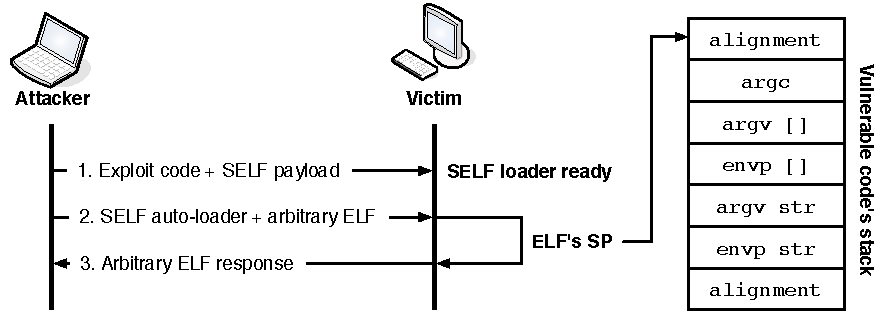
\includegraphics[width=\textwidth]{figures/host/forensics/self_new}
 \caption{An illustration of the in-memory execution technique.}
 \label{fig:self}
\end{figure}

Even in this evaluation, we used the dataset described in
Section~\ref{host:experimental-setup}. However, a slight modification
of the generation mechanism was needed. More precisely, in the tests
conducted we used a modified version of SELF \citep{SELF-TOOL}, which
we improved in order to reliably run under \textsf{FreeBSD}\index{FreeBSD} 6.2 and
ported to a form which could be executed through code injection (i.e.,
to shellcode\index{shellcode} format). SELF implements a technique known as
\emph{userland exec}: it modifies any statically linked
\ac{ELF}\index{ELF} binary and, by building a specially-crafted stack,
it allows an attacker to load and run that \ac{ELF}\index{ELF} in the
memory space of a target process without calling the kernel and, more
importantly, without leaving any trace on the hard disk of the
attacked machine. This is done through a two-stage attack where a
shellcode\index{shellcode} is injected in the vulnerable program, and then retrieves a
modified \ac{ELF}\index{ELF} from a remote machine, and subsequently
injects it into the memory space of the running target process, as
shown schematically in Figure \ref{fig:self}.

Eight experiments with both \texttt{eject} and \texttt{bsdtar}\index{bsdtar} were performed. Our anomaly detector was first trained with ten different execution of \texttt{eject} and more than a hundred executions of \texttt{bsdtar}\index{bsdtar}. We also audited eight instances of the activity of \texttt{eject} under attack, while for \texttt{bsdtar}\index{bsdtar} we logged seven malicious executions. We repeated the tests both with a simple shellcode\index{shellcode} which opens a root shell (a simple \texttt{execve} of \texttt{/bin/sh}) and with our implementation of the userland\index{userland} exec technique.

\begin{table}[t]
  \centering
  \begin{tabular}{rcccc}
    \toprule
    \emph{Executable} & \multicolumn{2}{c}{Regular shellcode} & \multicolumn{2}{c}{Userland exec}\\
    \cmidrule{2-5}
    & FPR     & DR     & FPR     & DR\\
    \midrule
    \texttt{eject}  & 0\%     & 75\% & 0\% & 100\%\\
    \texttt{bsdtar} & 7.81\%  & 71\% & 7.81\% & 100\%\\
    \bottomrule
  \end{tabular}
  \caption{Experimental results with a regular shellcode and with our userland exec implementation.}
  \label{tab:results}
\end{table}

The overall results are summarized in Table \ref{tab:results}. Let us consider the effectiveness of the detection of the attacks themselves. The attacks against \texttt{eject} are detected with no false positive at all. The exploit is detected in the very beginning: since a very long argument is passed to the \texttt{execve}, this triggers the argument model. The detection accuracy is similar in the case of \texttt{bsdtar}\index{bsdtar}, even if in this case there are some false positives. The detection of the shellcode\index{shellcode} happens with the first \texttt{open} of the unexpected special file \texttt{/dev/tty}. It must be underlined that most of the true alerts are correctly fired at system call level; this means that malicious \emph{calls} are flagged by our \ac{IDS}\index{IDS} because of their unexpected arguments, for instance.

On the other hand, exploiting the userland\index{userland} exec an attacker launches an otherwise normal executable, but of course such executable has different system calls, in a different order, and with different arguments than the ones expected in the monitored process. This reflects in the fact that we achieved a 100\% \ac{DR} with no increase in false positives, as each executable we have run through SELF has produced a Markov model which significantly differs from the learned one for the exploited host process.

\section{Concluding Remarks}
\label{host:conclusions}
In this chapter we first described in detail two contributions to host-based anomaly detection and then demonstrated how these techniques can be successfully applied to circumvent anti-forensics tools often used by intruders to avoid to leave traces on the file-system.

First, we described a host-based \ac{IDS}\index{IDS} based on the analysis of system calls arguments and sequences. In particular, we analyzed previous literature on the subject, and found that there exists only a handful of works which take into account the anomalies in such arguments. We improved the models suggested in one of these works, we added a stage of clustering in order to characterize normal invocations of calls and to better fit models to arguments, and finally we complemented it with Markov models in order to capture correlation between system calls. 

We showed how the prototype is able to correctly contextualize alarms, giving the user more information to understand what caused any false positive, and to detect variations over the execution flow, as opposed to punctual variations over single instances. We also demonstrated its improved detection capabilities, and a reduction of false positives. The system is auto-tuning and fully unsupervised, even if a range of parameters can be set by the user to improve the quality of detection.

A possible future extension of the technique we described is the analysis of complementary approaches (such as Markov model merging or the computation of distance metrics) to better detect anomalies in the case of long system call sequences, which we identified as a possible source of false positives. In the following section, we describe how a deterministic behavioral model, i.e., an \ac{FSA}\index{FSA}, often shows a better and more accurate characterization of the process flow. However, to achieve better \ac{FPR} of \ac{SSAADE} we had to add several stochastic models to avoid many false detections; this, as expected, is paid at the price of higher computational overheads.

Secondly, we demonstrated that a good alternative to using distance metrics between Markov models is the exploiting deterministic models for the control flow. More precisely, we showed how the deterministic dataflow relations between arguments implemented in FSA-DF can be improved by using better statistical models. In addition, we partially addressed the problem of spurious datasets by introducing a Gaussian string model, which has been shown to be more resilient to outliers (i.e. too long or too short strings). We also proposed a new model for counting the frequency of traversal of edges on FSA-DF, to make it able to detect \ac{DoS} attacks. Both systems needed an improved model for string (path) similarity. We adapted the Symbol \ac{SOM}\index{SOM} algorithm to make it suitable for computing a distance between two paths. We believe that this is the core contribution. 

We tested and compared the original prototypes with an hybrid solution where the Symbol \ac{SOM}\index{SOM} and the edge traversal models are applied to the \ac{FSA}\index{FSA}, and a version of \ac{SSAADE} enhanced with the Symbol SOM and the correction to the execution arguments model. Both the new prototypes have the \emph{same} \acp{DR}\index{DR} of the original ones, but significantly \emph{lower} \acp{FPR}\index{FPR}. This is paid in terms of a non-negligible limit to detection speed, at least in our proof of concept implementation.

Future efforts will focus on re-engineering the prototypes to use an in-kernel system call interceptor, and generically improve their performance. We are studying how to speed up the Symbol \ac{SOM}\index{SOM} node search algorithm, in order to bring the throughput to a rate suitable for online use.

Last, we analyzed the wide class of \emph{definitive} anti-forensics techniques which try to eliminate evidence by avoiding disk usage. In particular, we focused on in-memory injection techniques. Such techniques are widely used by modern attack tools (both commercial and open source). 

As memory dump and analysis is inconvenient to perform, often not part of standard operating procedures, and does not help except in case of in-memory resident backdoors\index{backdoors} and rootkits, we proposed an alternative approach to circumvent such techniques. We illustrated how a prototype which analyzes (using learning algorithms) the sequence and the arguments of system calls to detect intrusions can be used to detect in-memory injections of executable code, and in-memory execution of binaries.

We proposed an experimental setup using vulnerable versions of two widely used programs on \textsf{FreeBSD}\index{FreeBSD}, \texttt{eject} and \texttt{bsdtar}\index{bsdtar}. We described the creation of a training and testing dataset, how we adapted or created exploits for such vulnerabilities, and how we recorded audit data. We also developed an advanced in-memory execution payload, based on SELF, which implements the ``userland\index{userland} exec'' technique through an injectable shellcode\index{shellcode} and a self-loading object (a specially-crafted, statically linked \ac{ELF}\index{ELF} file). The payload executes any statically linked binary in the memory space of a target process without calling the kernel and, more importantly, without leaving any trace on the hard disk of the attacked machine. 

We performed several experiments, with excellent \acp{DR}\index{DR} for the \emph{exploits}, but even more importantly with a 100\% \ac{DR} for the in-memory execution payload itself. We can positively conclude that our technique yields promising results for creating a forensic audit trail of otherwise ``invisible'' injection techniques. Future developments will include a more extensive testing with different anti-forensics techniques, and the development of a specifically designed forensic output option for our prototype.

%%% Local Variables: 
%%% mode: latex
%%% TeX-master: "thesis"
%%% End: 

% LocalWords:  POSIX chmod IDEVAL mcweject bsdtar PAX libarchive shellcode mutz
% LocalWords:  FreeBSD libanomaly syscalls BSM OpenBSM openbsm dev myarchive

\chapter{Anomaly Detection of Web-based Attacks}
\label{web}
Anomaly detection techniques have been shown to be very effective at mitigating the widespread of malicious activity against web applications. In fact, nowadays, the underground criminals' preferred way of spreading malware\index{malware} consists in compromising vulnerable web applications, deploying a phishing-, spamming-, malware-kit\index{malware} and infecting an enormous amount of users that simply visit the website using a vulnerable browser (or plug-in). Further exacerbating the situation is the use of botnets\index{botnets} to exhaustively compromise vast amounts of web applications. Thus, due to their popularity, web applications play a significant role in the malware\index{malware} spreading work-flow. As a consequence, by blocking attacks against web applications the majority of potential infections can be avoided. Indirectly, all the visitors of the website benefit from the adoption of web-based \acp{IDS}\index{IDS}.

Unfortunately, even the most advanced anomaly detectors of web-based attacks are not with their drawbacks. In particular, in this chapter we discuss our contributions to overcome two relevant training issues, overfitting\index{overfitting} and concept-drift, that both manifest themselves as increased \acp{FPR}\index{FPR}. First, we address overfitting\index{overfitting} due to training data scarcity, which results in under-trained activity models with poor generalization capabilities. Consequently, a considerable amount of normal events is classified as malicious. Secondly, we propose a simple but extremely effective mechanism to detect changes in the monitored system to adapt the models to what we named web application concept drift.

\section{Preliminaries}
\label{web:intro}
The two contributions described in Section~\ref{web:longtail} and \ref{web:conceptdrift} are both based on the generic anomaly detection architecture described in the following. In this section, a generic model of an anomaly-based detector of attacks against web applications is given. In addition, the details of the datasets used to evaluate the effectiveness of both the approach are described.

\subsection{Anomaly Detectors of Web-based Attacks}
\label{web:intro:ad}
Unless differently stated, we use the shorthand term \emph{anomaly detector} to refer to anomaly-based detectors that leverage unsupervised machine learning techniques. Let us first overview the basic concepts.

Without loss of generality, a set of web applications $A$ can be organized into a set of \emph{resource paths} or \emph{components} $R$, and named \emph{parameters} $P$. For example, $A = \{a_{1}, a_{2}\}$ may contain a blog application $a_1=\mathtt{blog.example.com}$ and an e-commerce application $a_{2}=\mathtt{store.example.com}$. They can be decomposed into their resource paths:

\begin{displaymath}\footnotesize
  \begin{array}{cc}
    R_{1} = & R_{2} = \\
    \left\{
      \begin{array}{l}
        r_{1,1} = \mathtt{/article/},\\
        r_{1,2} = \mathtt{/comments/},\\
        r_{1,3} = \mathtt{/comments/edit/},\\
        r_{1,4} = \mathtt{/account/},\\
        r_{1,5} = \mathtt{/account/password/}
      \end{array}
    \right\}
    &
    \left\{
      \begin{array}{l}
        r_{2,1} = \mathtt{/list/},\\
        r_{2,2} = \mathtt{/cart/},\\
        r_{2,3} = \mathtt{/cart/add/},\\
        r_{2,4} = \mathtt{/account/},\\
        r_{2,5} = \mathtt{/account/password/}
      \end{array}
    \right\}
  \end{array}
\end{displaymath}

\noindent In this example, resource path $r_{1,5}$ might take a set of parameters, as part of the \ac{HTTP}\index{HTTP} request. For instance, the following request to $r_{1,5} = \mathtt{/account/password/}$

\begin{logs}
  GET /account/password/id/12/oldpwd/14m3/newpwd/1337/ HTTP/1.1
\end{logs}

\noindent can be parsed into the following abstract data structure:

\begin{displaymath}
  P_{1,5}=\left\{
    \begin{array}{rlrl}
        \langle p_{1,5,1} =& \mathtt{id} & v_{1,5,1} =& \mathtt{12}\rangle,\\
        \langle p_{1,5,2} =& \mathtt{oldpw} & v_{1,5,2} =& \mathtt{14m3}\rangle,\\
        \langle p_{1,5,3} =& \mathtt{newpw} & v_{1,5,3} =& \mathtt{1337}\rangle
    \end{array}
  \right\}.
\end{displaymath}

A generic web application \ac{IDS} based on unsupervised learning
techniques captures the system activity $\mathbb{I}$ as a sequence of
\emph{requests} $Q = \left\{q_1, q_2, \ldots \right\}$, similar to
those exemplified in Section~\ref{detection:id}, issued by web clients
to the set of monitored web applications. Each request $q \in Q$ is
represented by a tuple $\left\langle a_i,r_{i,j},P_q \right\rangle$,
where $P_q$ is a set of parameter name-value pairs such that $P_q
\subseteq P_{i,j}$.

During the initial \emph{training phase}, the anomaly detection system
learns the characteristics of the monitored web applications in terms
of \emph{models}.  As new web application, resource path, and
parameter instances are observed, the sets $A$, $R$, and $P$ are
updated. For each unique parameter $p_{i,j,k}$ observed in association
with a particular application $a_i$ and path $r_{i,j}$, a set of
models that characterize the various features of the parameter is
constructed.  An activity profile
(Definition~\ref{def:activity-model}) associated with each unique
parameter instance is generated $c_{\left(.\right)} = \left\langle
  m^{(1)},m^{2},\ldots,m^{(u)},\ldots,m^{(U)} \right\rangle$, which we
name \emph{(parameter) profile} or \emph{model composition}.
Therefore, for each application $a_i$ and resource path $r_{i,j}$, a
set $\mathcal{C}_{i,j}$ of model compositions is constructed, one for
each parameter $p_{i,j,k}\in P_{i,j}$.  The \emph{knowledge base} of
an anomaly detection system trained on web application $a_i$ is
denoted by $\mathcal{C}_{a_i}=\bigcup_{j}\mathcal{C}_{i,j}$.  A
graphical representation of how a knowledge base is modeled for
multiple web applications is depicted in Figure~\ref{fig:profiles}.

\begin{example}\label{ex:web-models}
  In \webanomaly, a profile for a given parameter $p_{i,j,k}$ is the
  following tuple:

  \begin{displaymath}
    c_{i,j,k}=\langle \mtok, \mint, \mlen, \mchar, \mstruct \rangle.
  \end{displaymath}

  \noindent Similarly to \LibAnomaly:

  \begin{itemize}
  \item [$\mtok$] models parameter values as a set of legal tokens
    (i.e., the set of of possible values for the parameter
    \texttt{gender}, observed during training).
  \item [$\mint$] and $\mlen$ describe normal intervals for literal
    integers and string lengths, respectively, using the Chebyshev\index{Chebyshev}
    inequality.
  \item [$\mchar$] models the character strings as a ranked frequency
    histogram, named \ac{ICD}, that are compared using the $\chi^2$ or
    G tests.
  \item [$\mstruct$] models sets of character strings by inducing a
    \ac{HMM}. The \ac{HMM}\index{HMM} encodes a probabilistic grammar
    that represents a superset of the strings observed in a training
    set. Aside from the addition of $\mint$, which is a
    straightforward generalization of $\mlen$ to numbers, the
    interested reader may refer to~\citep{kruegel:jcn2005:webanomaly}
    for further details.
  \end{itemize}
\end{example}

\begin{figure}[p]
  \centering
  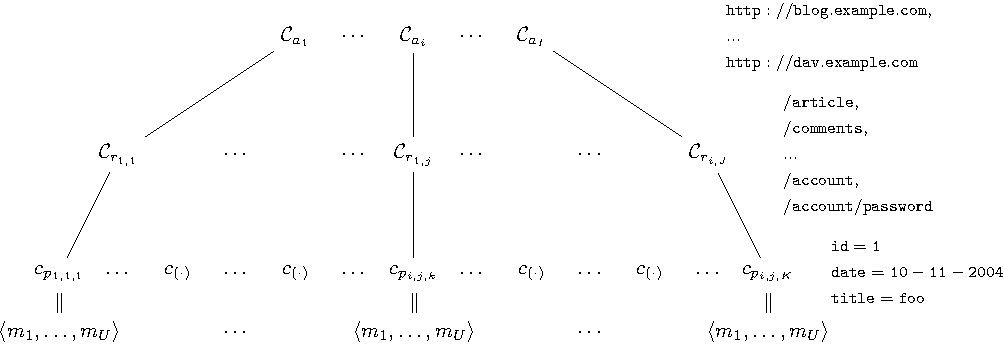
\includegraphics[angle=-90,width=.6\textwidth]{figures/web/profiles}
  \caption{Overview of web application model construction.}
  \label{fig:profiles}
\end{figure}

In addition to requests, the structure of user sessions can be taken
into account to model the normal states of a server-side
application. In this case, the anomaly detector does not consider
individual requests independently, but models their sequence. This
model captures the legitimate order of invocation of the resources,
according to the application logic. An example is when a user is
required to invoke an authentication resource (e.g.,
\texttt{/user/auth}) before requesting a private page (e.g.,
\texttt{/user/profile}). In~\citep{kruegel:jcn2005:webanomaly}, a
session $S$ is defined as a sequence of resources in $R$. For
instance, given $R = \{r_{1}, r_{2}, \dots, r_{10}\}$, a sample
session is $S = \langle r_{3}, r_{1}, r_{2}, r_{10}, r_{2}\rangle$.

Some systems also model \ac{HTTP}\index{HTTP} responses that are
returned by the server. For example,
in~\citep{kruegel:jcn2005:webanomaly}, a model $\mdoc$ is presented
that takes into account the structure of documents (e.g.,
\ac{HTML}\index{HTML}, \ac{XML}\index{XML}, and \ac{JSON}\index{JSON})
in terms of partial trees that include security-relevant nodes (e.g.,
\texttt{<script />} nodes, nodes containing \ac{DOM}\index{DOM} event
handlers, and nodes that contain sensitive data such as credit card
numbers). These trees are iteratively merged as new documents are
observed, creating a superset of the allowed document structure and
the positions within the tree where client-side code or sensitive data
may appear. A similar approach is adopted
in~\citep{masibty}.

\begin{note}[Web Application Behavior]
  The concept of \emph{web application behavior}, used in the
  following, is a particular case of the system behavior as defined by
  Definition~\ref{def:system-behavior}. Depending on the accuracy of
  each model, the behavior of a web application reflects the
  characteristics and functionalities that the application offers and,
  as a consequence, the content of the inputs (i.e., the requests)
  that it process and the outputs (i.e., the responses) that it
  produces. Thus, unless differently stated, we use the same term to
  indicate both the ideas.
\end{note}

After training, the system is switched to \emph{detection mode}, which
is performed online. The models trained in the previous phase are
queried to determine whether or not the new parameters observed are
anomalous. Without going into the details of a particular
implementation, each parameter is compared to all the applicable
models and an aggregated anomaly score between 0 and 1 is calculated
by composing the values returned by the various models. If the anomaly
score is above a certain threshold, an alert is generated. For
example, in~\citep{kruegel:acsac2003:bayesian}, the anomaly score
represents the probability that a parameter value is anomalous and it
is calculated using a Bayesian network that encodes the probability
that a parameter value is actually normal or anomalous given the
scores returned by the individual models.

\subsection{A Comprehensive Detection System to Mitigate Web-based
  Attacks}
\label{web:intro:masibty}
The approach described in~\citep{kruegel:jcn2005:webanomaly} are
further exploited in a recent work, \citep{masibty}, which we
partially contributed to. In particular, we defined a web application
anomaly detector that is able to detect a real-world threats against
the clients (e.g., malicious \textsf{JavaScript}\index{JavaScript} code, trying to
exploit browser vulnerabilities), the application (e.g., cross-site
scripting, permanent content injection), and the database layer (e.g.,
SQL injection). A prototype of the system, called \masibty, has been
evaluated on a set of real-world attacks against publicly available
applications, using both simple and mutated versions of exploits, in
order to assess the resilience to evasion. \masibty has the following
key characteristics:

\begin{itemize}
\item its models are designed with the explicit goal of not requiring
  an attack-free dataset for training, which is an unrealistic
  requirement in real-world applications. Even if in
  \citep{10.1109/SP.2008.11} techniques are suggested to filter
  outliers (i.e., attacks) from the training data, in absence of a
  ground truth there can be no guarantee that the dataset will be
  effectively free of attacks. Using such techniques before training
  \masibty would surely improve its detection capabilities.

\item As depicted in Figure~\ref{fig:masibty-architecture}, \masibty
  intercepts and process both HTTP requests (i.e., \emph{PAnomaly})
  and responses (i.e., \emph{XSS\-Anomaly}) and protects against both
  server-side and client-side attacks, an extremely important feature
  in the upcoming ``Web 2.0'' era of highly interactive websites based
  mainly on user contributed content. In particular, we devised two
  novel anomaly detection models --- referred to as ``engines'' ---
  based on the representation of the responses as trees.

\item \masibty incorporates an optional data protection component,
  i.e., \emph{QueryAnomaly} that extracts and parses the SQL queries
  sent to the database server. This component is part of the analysis
  of HTTP requests, and thus is not merely a reverse proxy to the
  database. In fact, it allows to bind the requests to the SQL queries
  that they generate, directly or indirectly. Hence, queries can be
  modeled although are not explicitly passed as a parameter of the
  HTTP requests.
\end{itemize}

\begin{figure}[p]
  \begin{center}
    \hspace*{2.5cm}
    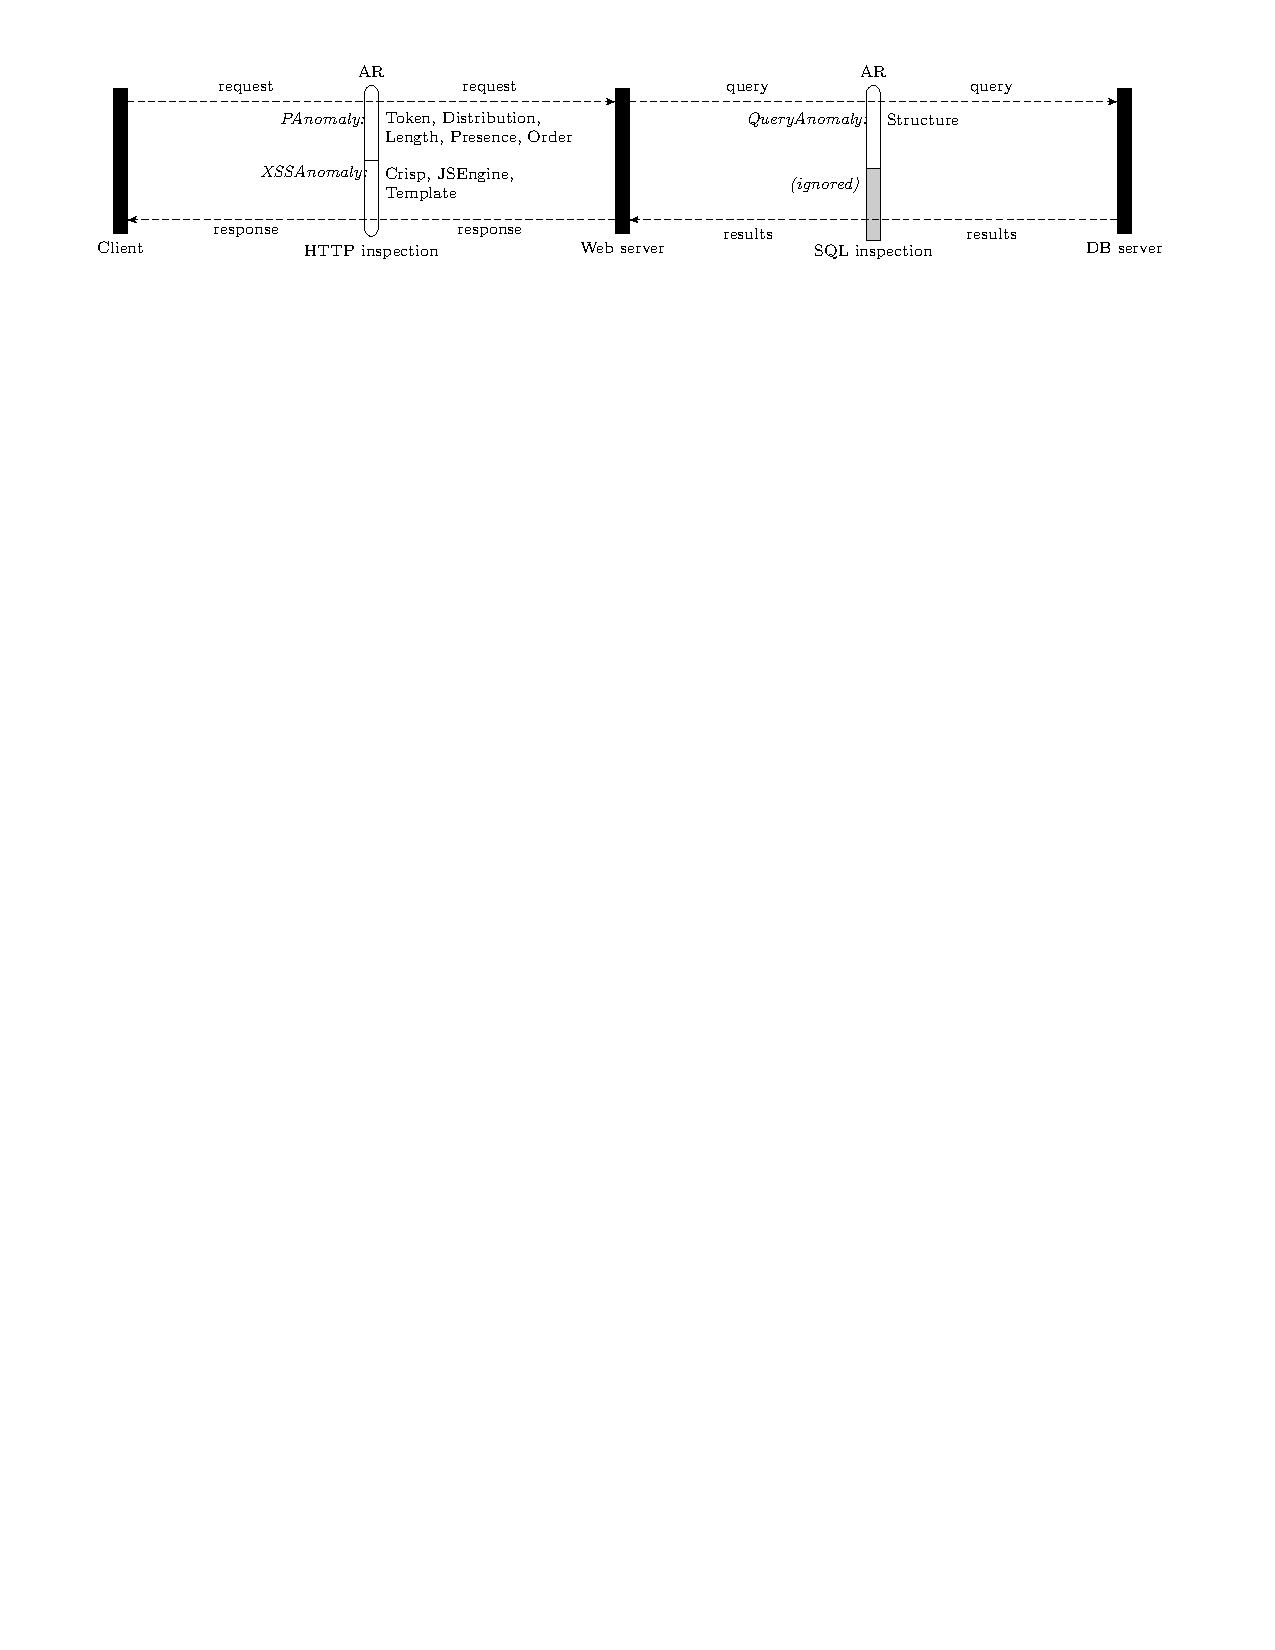
\includegraphics[angle=90,scale=.8]{figures/web/masibty/masibty-architecture}
  \end{center}

  \vspace*{-1cm}
  \caption{The logical structure of \masibty.}
  \label{fig:masibty-architecture}
\end{figure}

\subsection{Evaluation Data}
\label{web:intro:eval}
The experiments in Section~\ref{web:longtail} and \ref{web:conceptdrift} were conducted using a dataset drawn from real-world web applications deployed on both academic and industry web servers.  Examples of representative applications include payroll processors, client management, and online commerce sites.  For each application, the full content of each \ac{HTTP}\index{HTTP} connection observed over a period of several months was recorded.  The resulting flows were then filtered using the most advanced signature-based detection system, \textsf{Snort}\footnote{Source and attack signatures available for download at \url{http://snort.org}.}, to remove known attacks.  In total, the dataset contains 823 distinct web applications, 36,392 unique resource paths, 16,671 unique parameters, and 58,734,624 \ac{HTTP}\index{HTTP} requests.

\begin{note}[Dataset privacy]
  To preserve the privacy, the dataset used has been given to the Computer Security Laboratory of UC Santa Barbara under strict contractual agreements that denies to disclose specific information identifying the web applications themselves.
\end{note}

Two sets of 100,000 and 1,000 attacks was introduced into the dataset used for the approach described in Section~\ref{web:longtail} and \ref{web:conceptdrift}, respectively. These attacks were real-world examples and variations upon \ac{XSS} (e.g., CVE-2009-0781), \ac{SQL} injections (e.g., CVE-2009-1224), and command execution exploits (e.g., CVE-2009-0258) that manifest themselves in request parameter values, which remain the most common attacks against web applications. Representative examples of these attacks include:

\begin{itemize}
\item malicious JavaScript\index{JavaScript} inclusion
\begin{lstlisting}[numbers=none]
  <script src="http://example.com/malware.js"></script>
\end{lstlisting}
\item bypassing login authentication
\begin{lstlisting}[numbers=none]
  ' OR 'x'='x'--
\end{lstlisting}
\item command injection
\begin{lstlisting}[numbers=none]
  cat /etc/passwd | mail attacker@gmail.com \#
\end{lstlisting}

\end{itemize}

More precisely, the \ac{XSS}\index{XSS} attacks are variations on those listed in \citep{xss_cheat_sheet}, the \ac{SQL}\index{SQL} injections were created similarly from \citep{sqli_cheat_sheet}, and the command execution exploits were variations of common command injections against the \textsf{Linux} and \textsf{Windows} platforms.

\section{Training With Scarce Data}
\label{web:longtail}
In this section, we describe our contributions \citep{2009_robertson_maggi_kruegel_vigna} to cope with the difficulty of obtaining sufficient \emph{amounts} of training data. As we explained in Section~\ref{detection:ad:host} and \ref{detection:evaluation:issues}, this limitation has heretofore not been well studied. We developed this technique to work with \webanomaly and, in general, to any learning-based anomaly detection system against web attacks. In fact, the problem described in the following is significantly evident in the case of web applications. However, it can be easily applied to other anomaly-based system, as long as they rely on behavioral models and learning techniques such as those described in Section~\ref{host:syscall}.

The issue that motivates this work is that the number of web application component invocations is non-uniformly distributed. In fact, we noticed that relatively few components are dominant in the traffic and the remainder components are accessed relatively infrequently. Therefore, for those components, it is difficult to gather enough training data to accurately model their normal behavior.  In statistics, the infrequently accessed population is known as the ``long tail''. Note that, however, this does not necessarily imply a power law distribution. Clearly, components that are infrequently accessed lead to undertrained models (i.e., models that do not capture the normal behavior accurately). Consequently, models are subject to overfitting\index{overfitting} due to lack of data, resulting in increases in the \ac{FPR}.

In particular, in this section, we describe our joint work with UC Santa Barbara in which we propose to mitigate this problem by exploiting natural similarities among all web applications. In particular, we show that the values of the parameters extracted from \ac{HTTP}\index{HTTP} requests can generally be categorized according to their type, such as an integer, date, or string.  Indeed, our experiments demonstrate that parameters of similar type induce similar models of normal behavior.  This result is then exploited to supplement a local scarcity of training data for a given web application component with similar data from other web applications.

This section is structured as follows. In Section~\ref{web:longtail:motivation} the problem of the non-uniform distribution to the different components of a web application is discussed. In addition, we provide evidence that it occurs in the real world. In Section~\ref{web:longtail:design} approach to address the problem of model profile undertraining\index{undertraining} by using the notion of \emph{global profiles} that exploit similarities between web application parameters of similar type. In Section~\ref{web:longtail:eval} the application of global profiles is evaluated on a large dataset of real-world traffic from many web applications, and demonstrate that utilizing global profiles allows anomaly detectors to accurately model web application components that would otherwise be associated with undertrained models.

\subsection{Non-uniformly distributed training data}
\label{web:longtail:motivation}
To describe the undertraining\index{undertraining} problem, in this section we refer to the aforementioned, generic architecture of a web-based anomaly detector. To address the problem of undertraining\index{undertraining}, we leverage the set of models described in the Example~\ref{ex:web-models}.

Because anomaly detection systems dynamically learn specifications of
normal behavior from training data, it is clear that the quality of
the detection results critically relies upon the quality of the
training data. For example, as mentioned in
Section~\ref{detection:evaluation:issues}, a training dataset should
be attack-free and should accurately represent the normal behavior of
the modeled features. To our knowledge, the difficulty of obtaining
sufficient amounts of training data to accurately model web
applications is less well-known. In a sense, this issue is similar to
those addressed by statistical analysis methods with missing
data~\citep{little1987statistical}. Although a training procedure would
benefit from such mechanisms, they require a complete redesign of the
training algorithm specific to each model. Instead, a non-obtrusive
approach that can improve an existing system without modifying the
undertrained models is more desirable.  Typically, anomaly-based
detectors cannot assume the presence of a testing environment that can
be leveraged to generate realistic training data that exercises the
web application in a safe, attack-free environment. Instead, an
anomaly detection system is typically deployed in front of live web
applications with no \emph{a priori} knowledge of the applications'
components and their behavior.

In particular, in the case of low-traffic web applications, problems
arise if the rate of client requests is inadequate to allow models to
train in a timely manner. Even in the case of high-traffic web
applications, however, a large subset of resource paths might fail to
receive enough requests to adequately train the associated models.
This phenomenon is a direct consequence of the fact that resource path
invocations issued by web clients often follow a non-uniform
distribution.  To illustrate this point, Figure~\ref{fig:long_tail}
plots the normalized cumulative distribution function of web client
resource path invocations for a variety of real-world, high-traffic
web applications (details on the source of this data are provided in
Section~\ref{web:longtail:eval}). Although several applications have
an approximately uniform client access distribution, a clear majority
exhibits highly skewed distributions.  Indeed, in many cases, a large
percentage of resource paths receive a comparatively minuscule number
of requests. Thus, returning to the example mentioned in
Section~\ref{web:intro:ad}, assuming an overall request volume of
500,000 requests per day, the resource path set would result in the
client access distribution detailed in
Table~\ref{tab:client-access-distribution}.

\begin{table}[t]
  \centering
  \begin{tabular}{rl}
    \toprule
    \textsc{Resource Path} & \textsc{Requests}\\
    \midrule

    \texttt{/article} & 95.0\% \\
    \texttt{/comments} & 3.0\% \\
    \texttt{/comments/edit} & 1.8\% \\
    \texttt{/account} & 0.2\% \\
    \texttt{/account/password} & 0.02\%\\
    \bottomrule
  \end{tabular}

  \caption{Client access distribution on a real-world web application (based on 500,000 requests per day).}
  \label{tab:client-access-distribution}
\end{table}

Profiles for parameters to resource paths such as \texttt{/article} will receive ample training data, while profiles associated with account components will be undertrained. The impact of the problem is also magnified by the fact that components of a web application that are infrequently exercised are also likely to contain a disproportionately large portion of security vulnerabilities.  This could be a consequence of the reduced amount of testing that developers invariably perform on less prominent components of a web application, resulting in a higher rate of software flaws.  In addition, the relatively low request rate from users of the web application results in a reduced exposure rate for these flaws.  Finally, when flaws are exposed and reported, correcting the flaws may be given a lower priority than those in higher traffic components of a web application.

\begin{figure}[t]
  \centering
  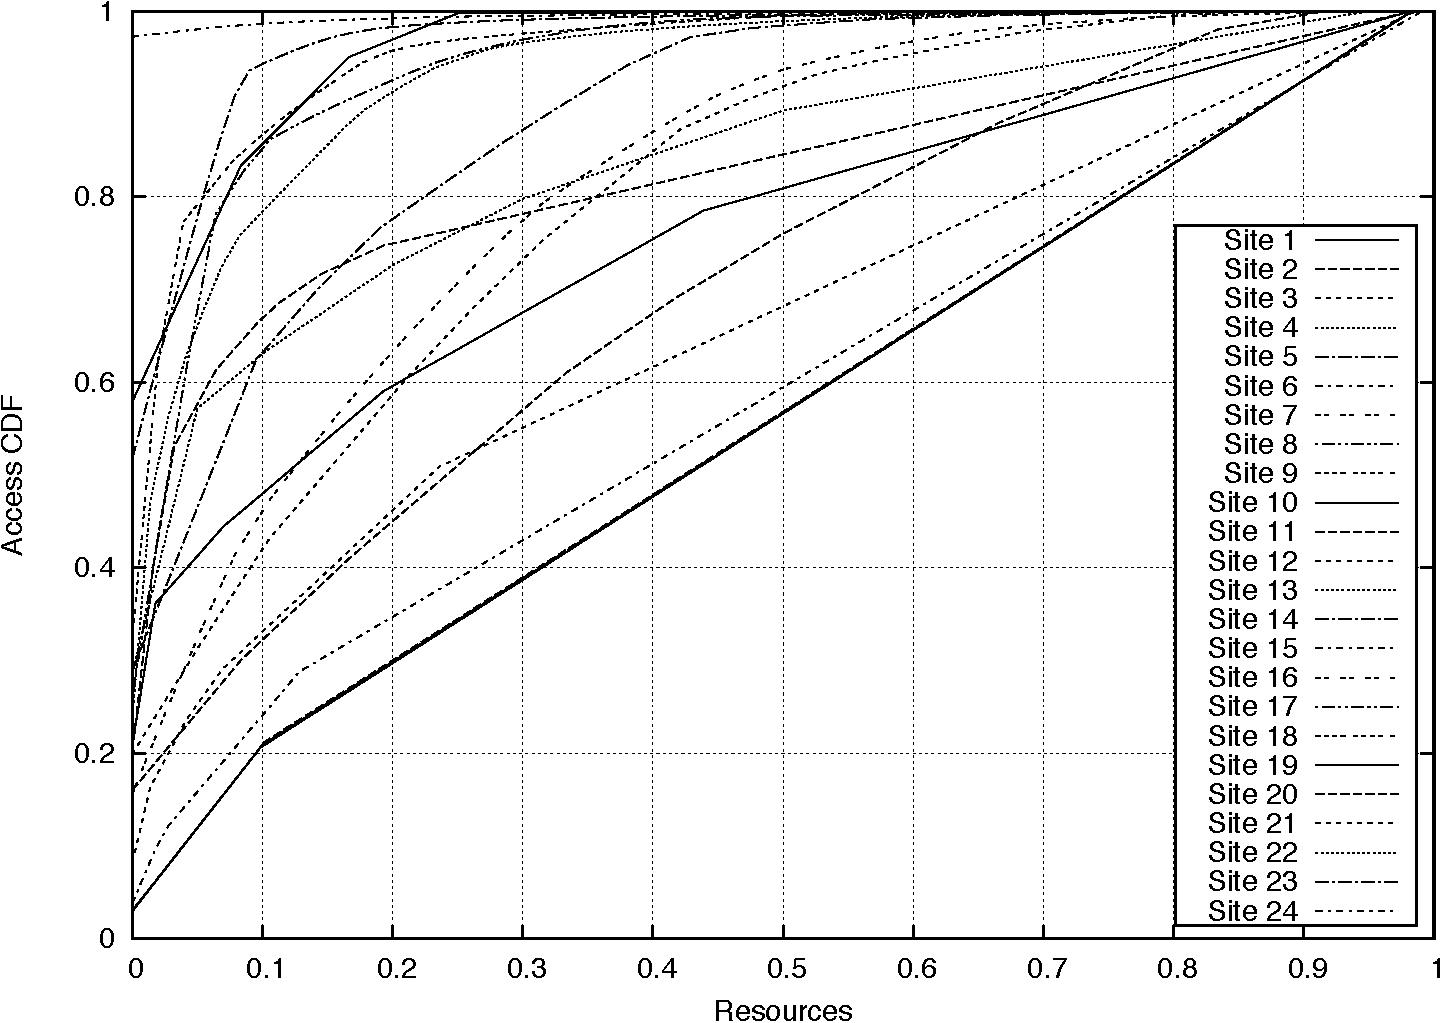
\includegraphics[width=.85\textwidth]{figures/web/longtail/fig_long_tail}
  \caption{Web client resource path invocation distributions from a
    selection of real-world web applications.}
  \label{fig:long_tail}
\end{figure}

\subsection{Exploiting global knowledge}
\label{web:longtail:design}
The approach described in this section is based on a key observation: parameters associated with the invocation of components belonging to different web applications often exhibit a marked similarity to each other. For instance, many web applications take an integer value as a unique identifier for a class of objects such as a blog article or comment, as in the case of the \texttt{id} parameter.  Similarly, applications also accept date ranges similar to the \texttt{date} parameter as identifiers or as constraints upon a search request.  Similarly, as in the case of the \texttt{title} parameter, web applications often expect a short phrase of text as an input, or perhaps a longer block of text in the form of a comment body. In some sense, each of these groupings of similar parameters can be considered as distinct \emph{parameter types}, though this need not necessarily correspond to the concept of types as understood in the programming languages context.

Our approach is based in the following assumption. Parameters of the
same type tend to induce model compositions that are similar to each
other in many respects. Consequently, if the lack of training data for
a subset of the components of a web application prevents an anomaly
detection system from constructing accurate profiles for the
parameters of those components, we claim that it is possible to
substitute, with an acceptably low decrease in the \ac{DR}, profiles
for similar parameters of the same type that were learned when enough
training data was available to construct accurate profiles. It must be
underlined that the substitution operates at the granularity of
\emph{parameters} rather than \emph{requests} (which may contain more
than one parameter). This increases the likelihood of finding
applicable profile similarities, and allows for the substitution of
models taken from radically different components.  However, although
the experiments on real-world data, described in
Section~\ref{web:longtail:eval}, confirm that the aforementioned
insight is realistic, our hypothesis might not hold in some very
specific settings. Thus, to minimize the risks brought by migrating
global knowledge across different deployments, we interpreted this
result only as an insight and developed a robust criterion able to
find similar profiles independently from the actual types of the
modeled parameters.

\begin{figure*}
  \centering
  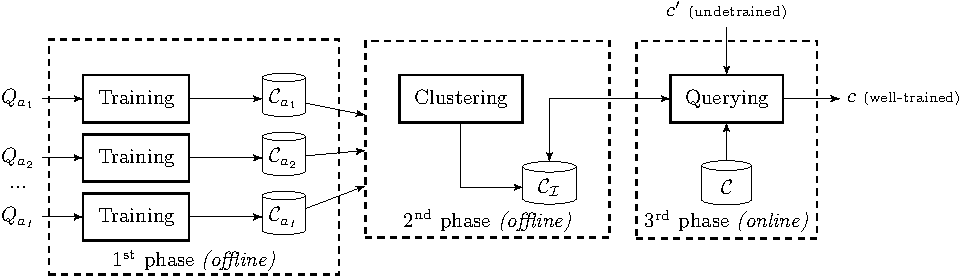
\includegraphics[width=\textwidth]{figures/web/longtail/overview}

  \caption{Overall procedure. Profiles, both undertrained and well-trained, are collected from a set of web applications. These profiles are processed offline to generate the global knowledge base $\kb$ and index $\kb^I$. $\kb$ can then be queried to find similar global profiles.}
  \label{fig:overview}
  
  \vspace*{-.4cm}
\end{figure*}

As schematized in Figure~\ref{fig:overview} our approach is composed of three phases.

\begin{description}
\item [First phase] (offline) Enhancement of the training procedure originally implemented in~\citep{kruegel:jcn2005:webanomaly}.

\item[Second phase] (offline) It is divided into three sub-steps.

  \begin{enumerate}
  \item A \emph{global knowledge base} of profiles $\kb=\bigcup_{a_i}\kb_{a_i}$ is constructed, where $\kb_{a_i}$ are knowledge bases containing only well-trained, stable profiles from anomaly detection systems previously deployed on a set of web applications $\bigcup_{i}a_i$.
  \item A knowledge base $\kb^I=\bigcup_{a_i}\kb_{a_i}^I$ of undertrained profiles is then constructed as an \emph{index} into $\kb$, where $\kb_{a_i}^I$ is a knowledge base of undertrained profiles from the web application $a_i$.
  \item Finally, a \emph{mapping} $f:\left\{\kb^I\right\}\times\kb_{a_i}\mapsto\kb$ is defined.
  \end{enumerate}

\item[Third phase] (online) For any new web application where insufficient training data is available for a component's parameter, the anomaly detector first extracts the undertrained profile $c'$ from the local knowledge base $\kb_{a_i}$.  Then, the global knowledge base $\kb$ is queried to find a similar, previously constructed profile $f\left(\kb_I,c'\right)=c\in\kb$.  The well-trained profile $c$ is then substituted for the undertrained profile $c'$ in the detection process.
\end{description}

The following sections detail how $\kb_I$ and $\kb$ are constructed, and how $f$ maps elements in $\kb_I$ and $\kb_{a_i}$ to elements in $\kb$.

\subsubsection{First Phase: Enhanced Training}
\label{web:longtail:design:enhanced-training}
A significant refinement of the individual models described in~\citep{kruegel:jcn2005:webanomaly} is the criterion used to determine the length of the training phase.  An obvious choice is to fix a constant training length, e.g., a thousand requests.  Unfortunately, an appropriate training length is dependent upon the complexity of modeling a given set of features.  Therefore, we have developed an automated method that leverages two stop criteria, \emph{model stability} and \emph{model confidence}, to determine when a model has observed enough training samples to accurately approximate the normal behavior of a parameter.

\paragraph{Model Stability}
\label{web:longtail:design:enhanced-training:stability}
As new training samples are observed early in the training phase, the
state of a model typically exhibits frequent and significant change as
its approximation of the normal behavior of a parameter is updated.
Informally, in an information-theoretic sense, the average information
gain of new training samples is high.  As a model's state converges to
a more precise approximation of normal behavior, however, its state
exhibits infrequent and incremental changes.  In other words, the
information gain of new training samples approaches zero, and the
model stabilizes. Note that, we refer to the information gain as an
informal and intuitive concept to explain the rationale behind the
development of a sound model stability criterion. By no means we claim
that our procedure relies on the actual information gain to calculate
when a model converges to stability.

Each model self-assesses its stability during the training phase by maintaining a history of snapshots of its internal state.  At regular intervals, a model checks if the sequence of deltas between each successive historical state is monotonically decreasing and whether the degree of change drops below a certain threshold.  If both conditions are satisfied, then the model considers itself stable.  Let $\kappa_{\text{stable}}^{\left(u\right)}$ denote the number of training samples required for a model to achieve stability.  A profile is considered stable when all of its constituent models are stable.

\begin{definition}[Profile stability]
   Let $\kappa_{\text{stable}}$ be the number of training samples required for a single model to achieve stability. The \emph{aggregated stability} measure is defined as:

   \begin{equation}
     \kappa_{\text{stable}}=\max_{u\in
       U}\kappa_{\text{stable}}^{\left(u\right)}.
   \end{equation}
\end{definition}

The notion of model stability is also leveraged in the third phase, as detailed in Section~\ref{web:longtail:design:global}.

\begin{note}
  Instead of describing the internal stop criterion specific to each
  model, if any, we developed a model-agnostic minimization algorithm
  detailed in Section~\ref{web:longtail:design:mapping} (and evaluated
  in Section~\ref{web:longtail:eval:robustness}) that allows one to
  trade off detection accuracy against the number of training samples
  available.
\end{note}

\paragraph{Model Confidence}
\label{web:longtail:design:enhanced-training:confidence}
A related notion to model stability is that of \emph{model confidence}.  Recall that the goal of a model is to learn an abstraction of the normal behavior of a feature from the training data.  There exists a well-known tension in the learning process between accurately fitting the model to the data and generalizing to data that has not been observed in the training set.  Therefore, in addition to detecting whether a model has observed enough training samples to accurately model a feature, each model incorporates a self-confidence measure $z^{\left(u\right)}$ that represents whether the model has generalized so much as to lose all predictive power.

For example, the confidence of a token model should be directly related to the probability that a token set is present.

\begin{definition}[Token model confidence]
  The \emph{token model confidence} is defined as:

\begin{equation}
  z^{\left(\text{tok}\right)}=\tau=\frac{1}{2}+\frac{n_c-n_d}{4n\left(n-1\right)},
\end{equation}

where $n_c$ and $n_d$ are the number of concordant and discordant pairs, respectively, between the unique number of observed samples and the total number of samples observed at each training step, and $n$ is the total number of training samples.
\end{definition}

Note that, $z_{\mtok}$ is an adaptation of the $\tau$ coefficient~\citep{kendalltau}.

For the integer and length models, the generality of a particular model can be related to the statistical dispersion of the training set.

\begin{definition}[Integer model confidence]
  Given the observed standard deviation $\sigma$, minimum observed value $u$, and maximum observed value $v$, the \emph{confidence of an integer or length model} is defined as:

\begin{equation}
  z^{\left(\left\{\text{int,len}\right\}\right)}=
  \begin{cases}
    1-\frac{\sigma}{v-u} &\text{if } v-u>0 \\
    1 &\text{otherwise}
  \end{cases}.
\end{equation}
\end{definition}

The confidence of a character distribution model is determined by the variance of observed \acp{ICD}\index{ICD}.  Therefore, the confidence of this model is given by a similar construction as the previous one, except that instead of operating over observed values, the measure operates over observed variances.

\begin{definition}[Char. distr. model confidence]
  Given the standard deviation of observed variances $\sigma$, the minimum observed variance $u$, and the maximum observed variance $v$, the \emph{confidence of a character distribution model} is:

\begin{equation}
  z^{\left(\text{char}\right)}=
  \begin{cases}
    1-\frac{\sigma}{v-u} &\text{if } v-u>0 \\
    1 &\text{otherwise}
  \end{cases}.
\end{equation}
\end{definition}

Finally, the \ac{HMM}\index{HMM} induced by the structure model can be directly analyzed for generality.  We perform a rough estimate of this by computing the mean probability for any symbol from the learned alphabet to be emitted at any state.

\begin{definition}[Struct. model confidence]
  Given a structural model, i.e. an \ac{HMM}, specified by the tuple $\langle\mathbb{S},\mathbb{O},M_{\mathbb{S}\times\mathbb{S}}, P\left(\mathbb{S},\mathbb{O}\right),P\left(\mathbb{S}\right)\rangle$, where $\mathbb{S}$ is the set of states, $\mathbb{O}$ is the set of emissions, $M_{\mathbb{S}\times\mathbb{S}}$ is the state transition probability matrix, $P\left(\mathbb{S},\mathbb{O}\right)$ is the emission probability distribution over the set of states, and $P\left(\mathbb{S}\right)$ is the initial probability assignment, \emph{the structural model confidence}:

\begin{equation}
  z^{\left(\text{struct}\right)}=1-
  \frac{1}{\left|\mathbb{S}\right|\left|\mathbb{O}\right|}
  \sum_{i=1}^{\left|\mathbb{S}\right|}
  \sum_{j=1}^{\left|\mathbb{O}\right|}P\left(s_i,o_j\right).
\end{equation}
\end{definition}

At the end of this phase, for each web application $a_{i}$, the profiles are stored in the corresponding knowledge base $\kb_{a_{i}}$ and are ready to be processed by the next phase.

\subsubsection{Second Phase: Building a global knowledge base}
\label{web:longtail:design:global}
This phase is divided into the three sub-steps described in the following.

\paragraph{Well-trained profiles}
The construction of $\kb$ begins by merging a collection of knowledge bases $\left\{\kb_{a_1},\kb_{a_2},\ldots,\kb_{a_n}\right\}$ that have previously been built by a web application anomaly detector over a set of web applications $\bigcup_{i}a_i$.  The profiles in $\kb$ are then clustered in order to group profiles that are semantically similar to each other.  Profile clustering is performed in order to time-optimize query execution when indexing into $\kb$, as well as to validate the notion of parameter types.  In this work, an agglomerative hierarchical clustering algorithm using group average linkage was applied, although the clustering stage is, in principle, agnostic as to the specific algorithm.  For an in-depth discussion of clustering algorithms and techniques, we refer the reader to~\citep{clustering:survey}.

Central to any clustering algorithm is the distance function, which defines how distances between the objects to be clustered are calculated.  A suitable distance function must reflect the semantics of the objects under consideration, and should satisfy two conditions:

\begin{itemize}
\item the overall similarity (i.e., inverse of the distance) between elements within the same cluster is maximized, and
\item the similarity between elements within different clusters is minimized.
\end{itemize}

We define the distance between two profiles to be the sum of the distances between the models comprising each profile. More formally.

\begin{definition}[Profile distance]
  The \emph{distance between two profiles} $c_i$ and $c_j$ is defined as:

  \begin{equation}
    d\left(c_i,c_j\right)=\frac{1}{\left|c_i\bigcap c_j\right|}
    \sum_{m_i^{\left(u\right)},m_j^{\left(u\right)}\in c_i\bigcap c_j}
    \delta_u\left(m_i^{\left(u\right)},m_j^{\left(u\right)}\right),
    \label{eq:dist}
  \end{equation}
  
  where $\delta_u:\mathcal{M}_u\times\mathcal{M}_u\mapsto\left[0,1\right]$ is the distance function defined between models of type $u\in U=\left\{\text{tok}, \text{int}, \text{len}, \text{char}, \text{struct}\right\}$.
\end{definition}

The token model $\mtok$ is represented as a set of unique tokens observed during the training phase. Therefore, two token models $\mtok_i$ and $\mtok_j$ are considered similar if they contain similar sets of tokens.  More formally.

\begin{definition}[Token models distance]
  The \emph{distance function for token models} is defined as the Jaccard\index{Jaccard} distance~\citep{clustering:distance_metrics_survey}:

\begin{equation}
  \delta_{\text{tok}}\left(\mtok_i,\mtok_j\right)=
  1-\frac{\left|\mtok_i\bigcap\mtok_j\right|}{\left|\mtok_i\bigcup\mtok_j\right|}.
\end{equation}
\end{definition}

The integer model $\mint$ is parametrized by the sample mean $\mu$ and variance $\sigma$ of observed integers.  Two integer models $\mint_i$ and $\mint_j$ are similar if these parameters are also similar.

\begin{definition}[Integer models distance]
  The \emph{distance function for integer models} is defined as:

  \begin{equation}
    \delta_{\text{int}}\left(\mint_i,\mint_j\right)=
    \frac{\left\|\frac{\sigma_i^2}{\mu_i^2}-\frac{\sigma_j^2}{\mu_j^2}\right\|}
    {\frac{\sigma_i^2}{\mu_i^2}+\frac{\sigma_j^2}{\mu_j^2}}.
  \end{equation}
\end{definition}

\begin{note}[Length models distance]
  As the string length model is internally identical to the integer model, its distance function $\delta_{\text{len}}$ is defined similarly.
\end{note}

Recall that the character distribution model $\mchar$ learns the frequencies of individual characters comprising strings observed during the training phase.  These frequencies are then ranked and coalesced into a $n$ bins to create an \ac{ICD}\index{ICD}.  Two character distribution models $\mchar_i$ and $\mchar_j$ are considered similar if each model's \acp{ICD}\index{ICD} are similar. More formally.

\begin{definition}[Char. distr. models distance]
  The \emph{character distribution models distance} is defined as:
\begin{equation}
  \delta_{\text{char}}\left(\mchar_i,\mchar_j\right)=
  \sum_{l=0}^{n}\frac{\left\|b_i\left(l\right)-b_j\left(l\right)\right\|}
  {\max_{k=i,j}b_k\left(l\right)},
\end{equation}

where $b_i\left(k\right)$ is the value of bin $k$ for $\mchar_i$.
\end{definition}

The structural model $\mstruct$ builds an \ac{HMM}\index{HMM} by observing a sequence of character strings.  The resulting \ac{HMM}\index{HMM} encodes a probabilistic grammar that can produce a superset of the strings observed during the training phase.  The \ac{HMM}\index{HMM} is specified by the tuple $\langle\mathbb{S},\mathbb{O},M_{\mathbb{S}\times\mathbb{S}}, P\left(\mathbb{S},\mathbb{O}\right),P\left(\mathbb{S}\right)\rangle$.  Several distance metrics have been proposed to evaluate the similarity between \acp{HMM}\index{HMM}~\citep{hmm:metrics:1, hmm:metrics:2, hmm:metrics:3, hmm:metrics:4}.  Their time complexity, however, is non-negligible.  Therefore, we adopt a less precise, but considerably more efficient, distance metric between two structural models $\mstruct_i$ and $\mstruct_j$.

\begin{definition}[Struct. models distance]
  The \emph{structural models distance} is defined as the Jaccard\index{Jaccard} distance between their respective emission sets:

\begin{equation}
  \delta_{\text{struct}}\left(\mstruct_i,\mstruct_j\right)=
  1-\frac{\left|\mathbb{O}_i\bigcap\mathbb{O}_j\right|}
  {\left|\mathbb{O}_i\bigcup\mathbb{O}_j\right|}.
\end{equation}
\end{definition}

\paragraph{Undertrained profiles}
Once the global knowledge base $\kb$ has been built, the next step is to construct a knowledge base of undertrained models $\kb^I$.  This knowledge base is composed of profiles that have been deliberately undertrained on $\kappa\ll\kappa_{\text{stable}}$ for each of the web applications $a_i$.  Because each member of $\kb^I$ uniquely corresponds to a member in $\kb$ and undertrained profiles are built for each well-trained profile in $\kb$, a bijective mapping $f':\kb^I\mapsto\kb$ exists between $\kb^I$ and $\kb$.  Therefore, when a web application parameter is identified as likely to be undertrained, the corresponding undertrained profile $c'$ can be compared to a similar undertrained profile in $\kb^I$, which is then used to select a corresponding stable profile from $\kb$. This operation requires the knowledge base $\kb^{I}$ to be indexed. The construction of the indices relies on the notion of model stability, described in Section~\ref{web:longtail:design:enhanced-training:stability}.

\begin{figure}[t]
  \centering
  \begin{tikzpicture}[el/.style={circle,fill=black!75,inner sep=1pt,label={above right:#1}},every label/.style = {font=\footnotesize},every node/.style={font=\footnotesize},ci/.style={shape=rectangle,thin,draw,inner sep=2pt}]

    \foreach \p in {1, 2, ..., 7}
       \foreach \k in {1, 2, ..., 8}
         \node [el] at ($ (5.5,0) + .8*(\k,\p)$) (d_\k_\p) {};

     \foreach \p/\k in {1/1, 2/2, 3/4, 4/8, 5/16, 6/32, 7/64}
       \node at ($ (5.5,0) + .8*(0,\p)$) {$\kappa = \k$};

     \node [ci,fit=(d_1_1)] {}
      node [ci,fit=(d_2_1)] {}
      node [ci,fit=(d_4_1)] {}
      node [ci,fit=(d_5_1)] {}
      node [ci,fit=(d_6_1)] {}
      node [ci,fit=(d_7_1)] {};

      \node [ci,fit=(d_1_2) (d_2_2)] {}
       node [ci,inner sep=3.5pt,fit=(d_2_2) (d_3_2)] {}
       node [ci,fit=(d_4_2) (d_5_2)] {}
       node [ci,fit=(d_7_2) (d_8_2)] {};

     \node [ci,fit=(d_2_3) (d_3_3) (d_4_3) (d_5_3)] {}
      node [ci,inner sep=3.5pt,fit=(d_5_3) (d_6_3) (d_7_3) (d_8_3)] {};

      \node [ci,fit=(d_1_4) (d_8_4)] {};

     \node [rotate=90] at (13,3.25) {Requests in $Q^{\left(p\right)}$};

  \end{tikzpicture}
  \caption{Partitioning of the training set $Q$ for various $\kappa$.}
  \label{fig:slicing}
\end{figure}

The undertrained profiles that comprise $\kb^I$ are constructed using
the following procedure.  Let
$Q^{\left(p\right)}=\{q_1^{\left(p\right)},q_2^{\left(p\right)},\ldots\}$
denote a sequence of client requests containing parameter $p$ for a
given web application.  Over this sequence of requests, profiles are
deliberately undertrained on randomly sampled $\kappa$-sequences.
Each of the resulting profiles is then added to the set $\kb^I$.
Figure~\ref{fig:slicing} depicts this procedure for various $\kappa$.
Note that the random sub-sampling is performed with the goal of
inducing undertraining\index{undertraining} to show that clustering is feasible and leads
to the desired grouping even -- and especially -- in the presence of
undertraining\index{undertraining}.

Recall that $\kappa_{\text{stable}}$ is the number of training samples required for a profile to achieve stability.  Then, a profile is considered undertrained when the number of training samples it has observed, $\kappa$, is significantly less than the number required to achieve stability.  Therefore, an undertrained knowledge base $\kb^I$ is a set of profiles that have observed $\kappa$ samples such that $\kappa\ll\kappa_{\text{stable}}$.

The selection of an appropriate value for $\kappa$ is central to both
the efficiency and the accuracy of this process.  Clearly, it is
desirable to minimize $\kappa$ in order to be able to index into $\kb$
as quickly as possible once a parameter has been identified to be
subject to undertraining\index{undertraining} at runtime.  On the other hand, setting
$\kappa$ too low is problematic, as Figure~\ref{fig:clustering}
indicates.  For low values of $\kappa$, profiles are distributed with
relatively high uniformity within $\kb^I$, such that clusters in
$\kb^I$ are significantly different than clusters of well-trained
profiles in $\kb$.  Therefore, slight differences in the state of the
individual models can cause profiles that are close in $\kb^I$ to map
to radically different profiles in $\kb$.  As
$\kappa\rightarrow\kappa_{\text{stable}}$, however, profiles tend to
form meaningful clusters, and tend to approximate those found in
$\kb$.  Therefore, as $\kappa$ increases, profiles that are close in
$\kb^I$ become close in $\kb$ under $f$ -- in other words, $f$ becomes
\emph{robust} with respect to model semantics.

\begin{figure}[p]
  \centering 
  \begin{tikzpicture}[el/.style={circle,fill=black!75,inner sep=1pt,label={above right:#1}},every label/.style = {font=\footnotesize},every node/.style={font=\footnotesize},ci/.style={shape=rectangle,thin,draw,inner sep=2pt}]

    \node [el,label={above right:$c_{p_{1,1}}$}] at (0, 0) (1_p_1) {};
    \node [el,label={above right:$c_{p_{2,1}}$}] at (0.5, 0.75) (1_p_2) {};
    \node [el,label={above right:$c_{p_{3,1}}$}] at (0, 1.5) (1_p_3) {} ;
    \node [el,label={above right:$c_{p_{4,1}}$}] at (-0.5, 0) (1_p_4) {};
    \node [el,label={above right:$c_{p_{5,1}}$}] at (1, 0.5) (1_p_5) {}; 

    \node [el,label={above right:$c_{p_{6,1}}$}] at (0, 1) (1_p_6) {};
    \node [el,label={above right:$c_{p_{7,1}}$}] at (0.5, 1.75) (1_p_7) {};

    \node [el,label={above right:$c_{p_{8,1}}$}] at (-1, 1) (1_p_8) {};
    \node [el,label={above right:$c_{p_{9,1}}$}] at (-1.5, 1.6) (1_p_9) {};
    \node [el,label={above right:$c_{p_{10,1}}$}] at (-1.25, 1.4) (1_p_10) {};

     \foreach \k/\name/\l in {3/2/2, 6/4/4, 8.5/K/\kappa}
       \foreach \i in {1, 2, ..., 10}
         \node [el,label={above right:$c_{p_{\i,\l}}$}] at ($ (1_p_\i) + (-1/\k*rand,\k) $) (\name_p_\i) {};
    
    \foreach \i in {1, 2, ..., 10}
         \node [el,label={above right:$c_{p_{\i}}$}] at ($ (K_p_\i) + (0,3) $) (s_p_\i) {};

     \foreach \k/\name in {1/1, 3/2, 6/4, 8.5/K}
       \foreach \i in {1, 2, ..., 10}
         \foreach \j in {1, 2, ..., 10}
           \fill [black,opacity=.45] ($ (\name_p_\i) + 0.8/\k*(rand,rand) $) circle (.7pt);

     \foreach \from/\to in {1/2, 2/4, 4/K}
       \foreach \i in {1, 2, ..., 10}
         \draw [opacity=.35] (\from_p_\i) -- (\to_p_\i);

    \node [el,inner sep=1.5pt,label={above right:$\mathbf{c}$}] at ($(K_p_8) - (.4, .4) $) (p) {};
    \node [circle,draw=black,inner sep=10pt,fill=black,opacity=.18] at ($ (p) $) (pn) {};
    \draw [-stealth] (p) to ($ (pn) - (10pt,10pt) $) {} node at ($ (p) - (.1,.25) $) {};
    \node [circle,draw=black,inner sep=15pt,fill=black,opacity=.15] at ($ (p) $) (pnn) {};
    \draw [-stealth] (p) to ($ (pn) - (22pt,0) $) {} node at ($ (p) - (.25,-.2) $) {};

    \draw [-stealth,dashed] (p) to [bend left=25] ($ (s_p_8) - (0.25,0)$) {};

     \node [draw = black!35, inner sep=5pt, thin, ellipse, fit = (1_p_1) (1_p_2) (1_p_3) (1_p_4) (1_p_5) (1_p_6) (1_p_7) (1_p_8) (1_p_9) (1_p_10)]{};

     \node [draw = black!35, inner sep=0pt, thin, ellipse, fit = (2_p_8) (2_p_9) (2_p_10)]{};
     \node [draw = black!35, inner sep=0pt, thin, ellipse, fit = (2_p_4)]{};
     \node [draw = black!35, inner sep=0pt, thin, ellipse, fit = (2_p_1) (2_p_2) (2_p_3) (2_p_5) (2_p_6) (2_p_7)]{};

     \node [draw = black!35, inner sep=0pt, thin, ellipse, fit = (4_p_8) (4_p_9) (4_p_10)]{};
     \node [draw = black!35, inner sep=0pt, thin, ellipse, fit = (4_p_1) (4_p_4) (4_p_5)]{};
     \node [draw = black!35, inner sep=0pt, thin, ellipse, fit = (4_p_2) (4_p_3) (4_p_6) (4_p_7)]{};

     \node [draw = black!35, inner sep=0pt, thin, ellipse, fit = (K_p_8) (K_p_9) (K_p_10)] {};
     \node [draw = black!35, inner sep=0pt, thin, ellipse, fit = (K_p_6) (K_p_5) (K_p_2)] {};
     \node [draw = black!35, inner sep=0pt, thin, ellipse, fit = (K_p_1) (K_p_4)] {};
     \node [draw = black!35, inner sep=0pt, thin, ellipse, fit = (K_p_3) (K_p_7)] {};

     \node [draw = black!35, inner sep=0pt, thin, ellipse, fit = (s_p_8) (s_p_9) (s_p_10)] {};
     \node [draw = black!35, inner sep=0pt, thin, ellipse, fit = (s_p_6) (s_p_5) (s_p_2)] {};
     \node [draw = black!35, inner sep=0pt, thin, ellipse, fit = (s_p_1) (s_p_4)] {};
     \node [draw = black!35, inner sep=0pt, thin, ellipse, fit = (s_p_3) (s_p_7)] {};

     \foreach \i/\k in {-1/0, 2.5/1, 5.5/2, 8.25/4, 11/\kappa_{min}, 14/{\kappa_{stable} \gg \kappa_{min}}}
       \draw [black!40] (-3, \i) to (3, \i) {}
         node [color=black,right] {$\kappa = \k$};

     \node at (-3, 0.75) {$\mathcal{C}_{1}^{I}$};
     \node at (-3, 4) {$\mathcal{C}_{2}^{I}$};
     \node at (-3, 6.75) {$\mathcal{C}_{4}^{I}$};
     \node at (-3, 9.5) {$\mathcal{C}_{\kappa_{min}}^{I}$};
     \node [rotate=90] at (11, 9.5) {Well-trained};
     \node at (10, 9.5) {$\mathcal{C}$};

     \node at ($ (K_p_7) + (1,1) $) {};
     
   \end{tikzpicture}

  \caption{Procedure for building global knowledge base indices.}
  \label{fig:clustering}
  \vspace*{-.4cm}
\end{figure}

\begin{note}[Robustness]
  Our use of the term ``robustness'' is related, but not necessarily equivalent, to the definition of robustness in statistics (i.e., the property of a model to perform well even in the presence of small changes in the underlying assumptions).
\end{note}

\paragraph{Mapping undertrained profiles to well-trained profiles}
\label{web:longtail:design:mapping}
A principled criterion is required for balancing quick indexing against a robust profile mapping.  Accordingly, we first construct a candidate knowledge base $\kb_{\kappa}^I$ for a given $\kappa$, as in the case of the global knowledge base construction.  Then, we define a \emph{robustness metric} as follows.  Let $H^I=\bigcup_{i}h_i^I$ be the set of clusters in $\kb^I$, and $H=\bigcup_{i}h_i$ be the set of clusters in $\kb$.  Let $g:H^I\mapsto\mathbb{N}$ be a mapping from an undertrained cluster to the maximum number of elements in that cluster that map to the same cluster in $\kb$.  The robustness metric $\rho:\left\{\kb^I\right\}\mapsto\left[0,1\right]$ is then defined as

\begin{equation}
  \rho\left(\kb^I\right)=\frac{1}{\left|\kb^I\right|}\sum_{i}g\left(h_i^I\right).
\end{equation}

With this metric, an appropriate value for $\kappa$ can now be chosen as

\begin{equation}
  \kappa_{\text{min}}=\min_{\kappa}\left(\rho\left(\kb_{\kappa}^I\right)\geq \rho_{\text{min}}\right),
\end{equation}

where $\rho_{\text{min}}$ is a minimum robustness threshold.

With the construction of a global knowledge base $\kb$ and an undertrained knowledge base $\kb^I$, online querying of $\kb$ can then be performed.

\subsubsection{Third Phase: Querying and Substitution}
Given an undertrained profile $c'$ from an anomaly detector deployed over a web application $a_i$, the mapping $f:\left\{\kb^I\right\}\times\kb_{a_i}\mapsto\kb$ is defined as follows.  A nearest\hyp{}neighbor match is performed between $c'$ and the previously constructed clusters $H^I$ from $\kb^I$ to discover the most similar cluster of undertrained profiles.  This is done to avoid a full scan of the entire knowledge base, which would be prohibitively expensive due to the cardinality of $\kb^I$.

Then, using the same distance metric defined in Equation~\eqref{eq:dist}, a nearest-neighbor match is performed between $c'$ and the members of $H^I$ to discover the most similar undertrained profile $c^I$.  Finally, the global, well-trained profile $f'\left(c^I\right)=c$ is substituted for $c'$ for the web application $a_i$.

To make explicit how global profiles can be used to address a scarcity
of training data, consider the example introduced in
Section~\ref{web:intro:ad}.  Since the resource path
\texttt{/account/password} has received only 100 requests (see
Table~\ref{tab:client-access-distribution}: \texttt{/account/password}
has received $0.02\%$ of 500,000 total requests), the profiles for
each of its parameters
$\left\{\mathtt{id},\mathtt{oldpw},\mathtt{newpw}\right\}$ are
undertrained, as determined by each profile's aggregate stability
measure.  In the absence of a global knowledge base, the anomaly
detector would provide no protection against attacks manifesting
themselves in the values passed to any of these parameters.

If, however, a global knowledge base and index are available, the situation is considerably improved.  Given $\kb$ and $\kb^I$, the anomaly detector can simply apply $f$ for each of the undertrained parameters to find a well-trained profile from the global knowledge base that accurately models a parameter with similar characteristics \emph{from another web application}.  Then, these profiles can be substituted for the undertrained profiles for each of $\left\{\mathtt{id},\mathtt{oldpw},\mathtt{newpw}\right\}$.  As will be demonstrated in the following section, the substitution of global profiles provides an acceptable detection accuracy for what would otherwise be an unprotected component (i.e., without a global profile 0\% of the attacks against that component would be detected).

\begin{note}[HTTP parameters ``semantics'']
  It is important to underline that the goal of this approach is not
  that of understanding the types of the fields nor their
  semantic. However, if the system administrator and the security
  officer had enough time and skills, the use of manual tools such as
  live debuggers or symbolic execution engines may help to infer the
  types of the fields and, once available, this information may be
  exploited as a lookup criterion. Unfortunately, this would be a
  human-intensive task, thus far from being automatic.

  Instead, our goal is to find groups of similar models, regardless of
  what this may imply in terms of types. According to our experiments,
  similar models tend to be associated to similar types. Thus, in
  principle, our method cannot be used to infer the parameters' types
  but can certainly give insights about parameters with similar
  features.
\end{note}

\subsection{Experimental Results}
\label{web:longtail:eval}
The goal of this evaluation is three-fold.  First, we investigate the
effects of profile clustering, and support the hypothesis of parameter
types by examining global knowledge base clusters.  Then, we discuss
how the quality of the mapping between undertrained profiles and
well-trained profiles improves as the training slice length $\kappa$
is increased.  Finally, we present results regarding the accuracy of a
web application anomaly detection system incorporating the application
of a global knowledge base to address training data scarcity.

\subsubsection{Profile clustering quality}
\label{web:longtail:eval:clustering}

\begin{figure}[p]
  \centering
  \subfloat[][$\kappa = 64$] {
    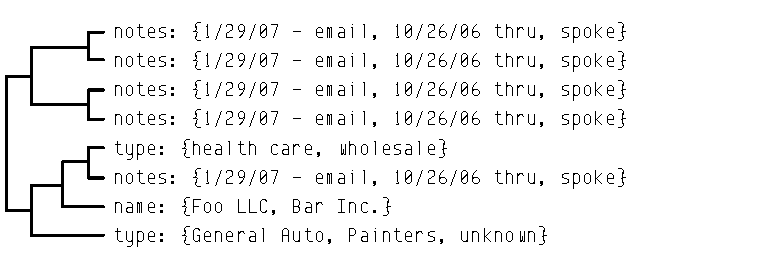
\includegraphics[scale=.5]{figures/web/longtail/undertrained-site-1-k-64-o}
    \label{subfig:undertrained-site-1-k-64}
  }\\
  \subfloat[][$\kappa_{stable} \simeq 10^{3}$] {
    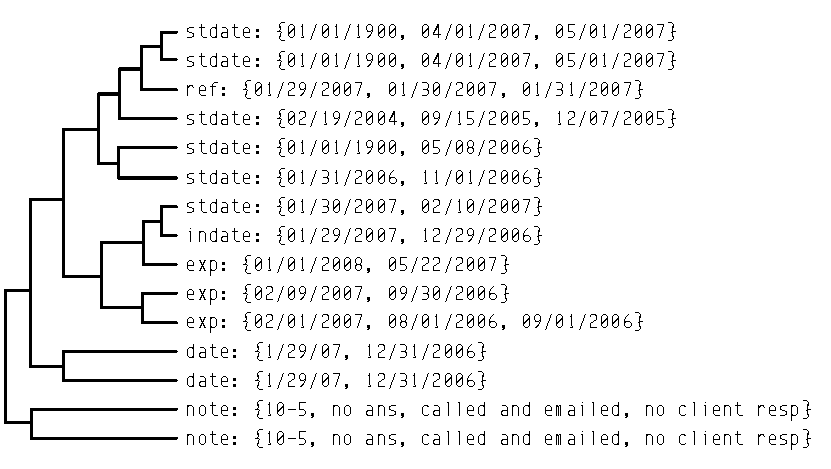
\includegraphics[scale=.5]{figures/web/longtail/undertrained-site-1-k-stable-o}
    \label{subfig:undertrained-site-1-k-stable}
  }\\
  \subfloat[][$\kappa = 8$]{
    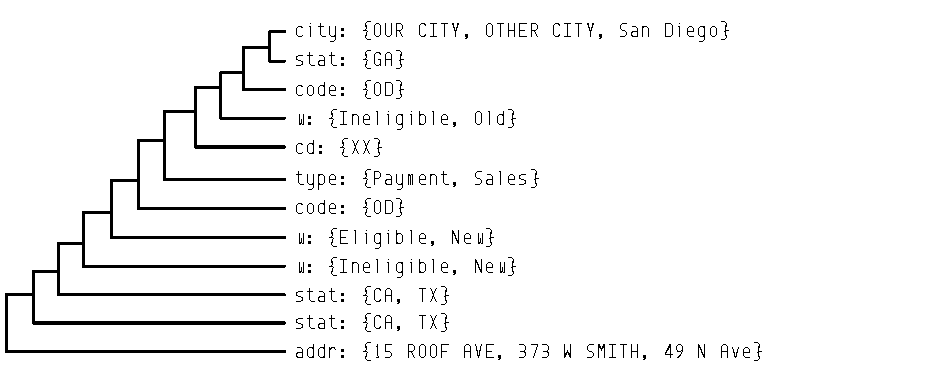
\includegraphics[scale=.5]{figures/web/longtail/undertrained-site-1-k-8-o}
    \label{subfig:undertrained-site-1-k-8}
  }\\
  \subfloat[][$\kappa = 32$]{
    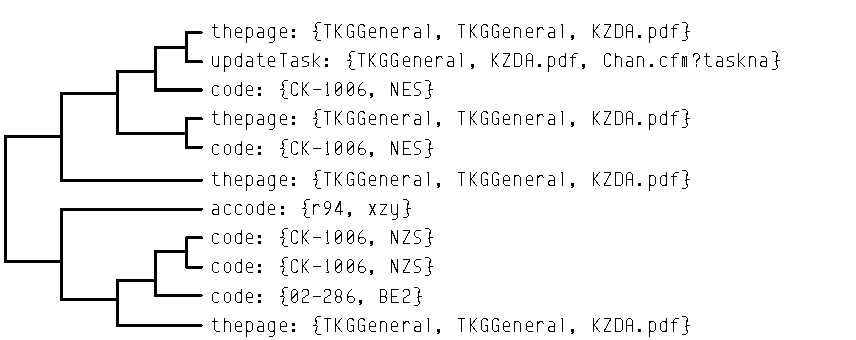
\includegraphics[scale=.5]{figures/web/longtail/undertrained-site-1-k-32-o}
    \label{subfig:undertrained-site-1-k-32}
  }\\
  \caption{Clustering of $\kb$, (a-b), and $\kb^I$, (c-d). Each leaf (a profile) is labeled with the parameter name and samples values observed during training. As $\kappa$ increases, profiles are clustered more accurately.}
  \label{fig:dendrograms}
  \vspace*{-.5cm}
\end{figure}

To evaluate the accuracy of the clustering phase, we first built a global knowledge base $\kb$ from a collection of well-trained profiles.  The profiles were trained on a subset of the data mentioned in Section~\ref{web:intro:eval}; this subset was composed of 603 web applications, 27,990 unique resource paths, 9,023 unique parameters, and 3,444,092 \ac{HTTP}\index{HTTP} requests.  The clustering algorithm described in Section~\ref{web:longtail:design:global} was then applied to group profiles according to their parameter type.  Sample results from this clustering are shown in Figure~\ref{subfig:undertrained-site-1-k-stable}.  Each leaf node corresponds to a profile and displays the parameter name and a few representative sample values corresponding to the parameter.

As the partial dendrogram indicates, the resulting clusters in $\kb$ are accurately clustered by parameter type.  For instance, date parameters are grouped into a single hierarchy, while unstructured text strings are grouped into a separate hierarchy.

The following experiment investigates how $\kappa$ affects the quality of the final clustering.

\subsubsection{Profile mapping robustness}
\label{web:longtail:eval:robustness}
Recall that in order to balance the robustness of the mapping $f$
between undertrained profiles and global profiles against the speed
with which undertraining\index{undertraining} can be addressed, it is necessary to select
an appropriate value for $\kappa$.  To this end, we generated
undertrained knowledge bases for increasing values of $\kappa=
1,2,4,8,16,32,64$ from the same dataset used to generate $\kb$,
following the procedure outlined in
Section~\ref{web:longtail:design:global}.  Partial dendrograms for
various $\kappa$ are presented in
Figure~\ref{subfig:undertrained-site-1-k-8},
\ref{subfig:undertrained-site-1-k-32},
\ref{subfig:undertrained-site-1-k-64}.

At low values of $\kappa$ (e.g.,
Figure~\ref{subfig:undertrained-site-1-k-8}), the clustering process
exhibits non-negligible systemic errors. For instance, the parameter
\texttt{stat} clearly should be clustered as a token set of states,
but instead is grouped with unstructured strings such as cities and
addresses.  A more accurate clustering would have dissociated the
token and string profiles into well-separated sub-hierarchies.

As shown in Figure~\ref{subfig:undertrained-site-1-k-32}, larger
values of $\kappa$ lead to more meaningful groupings. Some
inaccuracies are still noticeable, but the clustering process of the
sub-hierarchy is significantly better that the one obtained at $\kappa
= 8$. A further improvement in the clusters is shown in
Figure~\ref{subfig:undertrained-site-1-k-64}. At $\kappa = 64$, the
separation between dates and unstructured strings is sharper; except
for one outlier, the two types are recognized as similar and grouped
together in the early stages of the clustering process.

Figure~\ref{fig:robustness} plots the profile mapping robustness
$\rho(\cdot)$ against $\kappa$ for different cuts of the dendrogram,
indicated by $D_{\text{max}}$.  $D_{\text{max}}$ is a threshold
representing the maximum distance between two clusters. Basically, for
low $D_{\text{max}}$, the ``cut'' will generate many clusters with a
few elements; on the other hand, for high values of $D_{\text{max}}$
the algorithm will tend to form less clusters, each having a larger
number of elements. Note that this parameter is known to have two
different possible interpretations: it could indicate either a
threshold on the real distance between clusters, or a ``cut level'' in
the dendrogram constructed by the clustering algorithm. Although they
are both valid, we prefer to utilize the former.

Figure~\ref{fig:robustness} shows two important properties of our
technique. First, it demonstrates that the robustness is fairly
insensitive to $D_{\text{max}}$.  Second, the robustness of the
mapping increases with $\kappa$ until saturation at
$32\leq\kappa\leq64$.  This not only confirms the soundness of the
mapping function, but it also provides insights on the appropriate
choice of $\kappa_{min}$ to minimize the delay to global profile
lookup while maximizing the robustness of the mapping.

\begin{figure}[t]
  \centering
  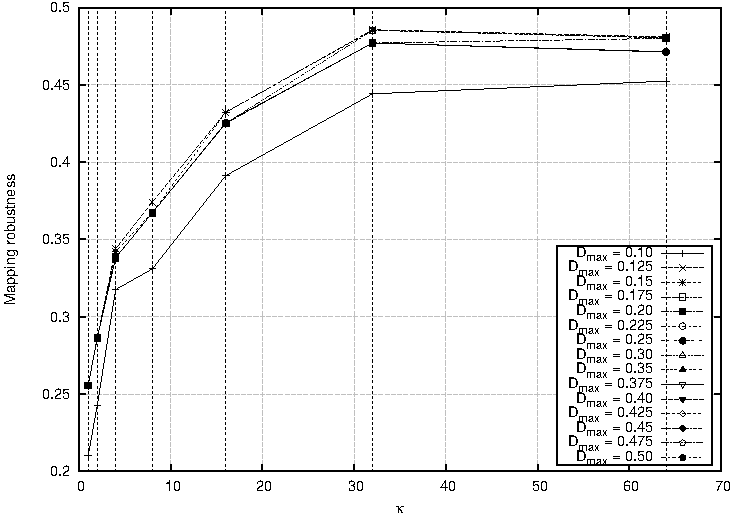
\includegraphics[width=.9\textwidth]{figures/web/longtail/fig_robustness}
  \caption{Plot of profile mapping robustness for varying $\kappa$.}
  \label{fig:robustness}
\end{figure}

\subsubsection{Detection accuracy}
\label{web:longtail:eval:detection}
Having studied the effects of profile clustering and varying values
for $\kappa$ upon the robustness of the profile mapping $f$, a
separate experiment was conducted in order to evaluate the detection
accuracy of a web application anomaly detector incorporating $\kb$,
the global knowledge base constructed in the previous experiments. In
particular, the goal of this experiment is to demonstrate that an
anomaly detector equipped with a global knowledge base exhibits an
improved detection accuracy in the presence of training data scarcity.

The data used in this experiment was a subset of the full dataset
described above, and was completely disjoint from the one used to
construct the global knowledge base and its indices.  It consisted of
220 unique real-world web applications, 8,402 unique resource paths,
7,648 distinct parameters, and 55,290,532 \ac{HTTP}\index{HTTP}
requests.

The intended threat model is that of an attacker attempting to
compromise the confidentiality or integrity of data exposed by a web
application by injecting malicious code in request parameters.

\begin{note}[Threat model]
  Although the anomaly detector used in this study is capable of
  detecting more complex session-level anomalies, we restrict the
  threat model to request parameter manipulation because we do not
  address session profile clustering.
\end{note}

To establish a worst-case bound on the detection accuracy of the
system, profiles for each observed request parameter were deliberately
undertrained to artificially induce a scarcity of training data for
\emph{all} parameters.  That is, for each value of
$\kappa=1,2,4,8,16,32,64$, the anomaly detector prematurely terminated
profile training after $\kappa$ samples, and then used the
undertrained profiles to query $\kb$.  The resulting global profiles
were then substituted for the undertrained profiles and evaluated
against the rest of the dataset.  The sensitivity of the system was
varied over the interval $\left[0,1\right]$, and the resulting
\ac{ROC}\index{ROC} curves for each $\kappa$ are plotted in
Figure~\ref{fig:roc}.

As one can clearly see, low values of $\kappa$ result in the selection
of global profiles that do not accurately model the behavior of the
undertrained parameters. As $\kappa$ increases, however, the quality
of the global profiles returned by the querying process increases as
well.  In particular, this increase in quality closely follows the
mapping robustness plot presented in Figure~\ref{fig:robustness}.  As
predicted, setting $\kappa=32,64$ leads to fairly accurate global
profile selection, with the resulting \ac{ROC}\index{ROC} curves
approaching that of fully-trained profiles.  This means that even if
the component of a web application has received only a few requests
(i.e., 64), by leveraging a global knowledge base it is possible to
achieve effective attack detection.  As a consequence, our approach
can improve the effectiveness of real-world web application firewalls
and web application anomaly detection systems.

Clearly, the detection accuracy will improve as more training samples
(e.g., 128, 256) become available. However, the goal of this
experiment was to evaluate such an improvement with a very limited
training set, rather than showing the detection maximum accuracy
achievable. From these results, we conclude that for appropriate
values of $\kappa$, the use of a global knowledge base can provide
reasonably accurate detection performance even in the presence of
training data scarcity.

\begin{figure}[t]
  \centering
  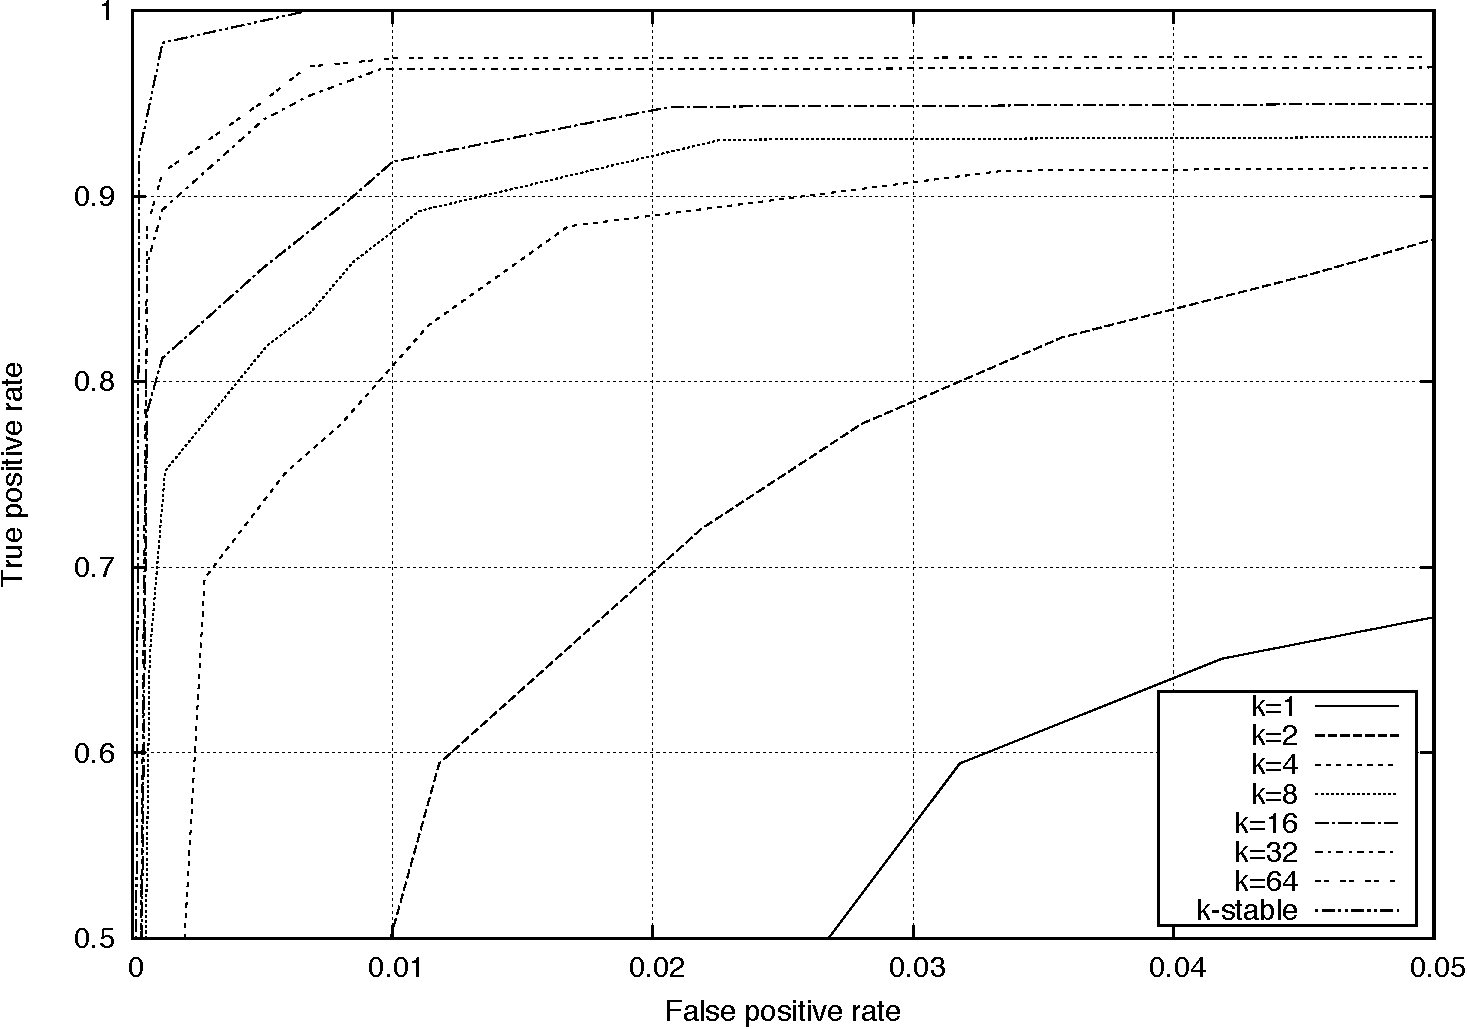
\includegraphics[width=.9\textwidth]{figures/web/longtail/fig_roc}
  \caption{Global profile ROC curves for varying $\kappa$. In the presence
    of severe undertraining ($\kappa \ll \kappa_{\text{stable}}$), the
    system is not able to recognize most attacks and also reports
    several false positives. However, as $\kappa$ increases, detection
    accuracy improves, and approaches that of the well-trained case
    ($\kappa=\kappa_{\text{stable}}$).}
  \label{fig:roc}
  \vspace*{-.5cm}
\end{figure}

One concern regarding the substitution of global profiles for local
request parameters is that a global profile that was trained on
another web application may not detect valid attacks against the
undertrained parameter.  Without this technique, however, recall that
a learning-based web application anomaly detector would otherwise have
no effective model whatsoever, and therefore the undertrained
parameter would be unprotected by the detection system (i.e., zero
true positive rate).  Furthermore, the \ac{ROC}\index{ROC} curves
demonstrate that while global profiles are in general not as precise
as locally-trained models, they do provide a significant level of
detection accuracy.

\begin{note}
  If global profiles were found to be as accurate as local profiles,
  this would constitute an argument against anomaly detection itself.
\end{note}

More precisely, with $\kappa = 1$, undertraining\index{undertraining} condition and system
off, only 67.5\% of the attacks are detected, overall, with around 5\%
of false positives. On the other hand, with $\kappa = 64$
(undertraining\index{undertraining} and system on), more than 91\% of the attacks are
detected with less than 0.2\% of false positives (\emph{vs.}, 0.1\% of
false positives in the case of no undertraining\index{undertraining} and system off).
Therefore, we conclude that, assuming no mistrust among the parties
that share the global knowledge base, our approach is a useful
technique to apply in the presence of undertrained models and, in
general, in the case of training data scarcity. Note that the last
assumption is often satisfied because one physical deployment (e.g.,
one server protected by our system) typically hosts several web
applications under the control of the same system administrator or
institution.

Therefore, we conclude that our approach is a useful technique to
apply in the presence of undertrained models and, in general, in case
of training data scarcity.

\begin{note}[Configuration parameters]
  Our methods provide explicit guidance, based on the training data of
  the particular deployment, to choose the value of the only parameter
  required to trade off accuracy \emph{vs.} length of the training
  phase. In addition, the ``goodness'' of the approach with respect to
  different choices of such a parameter is evaluated on real-world
  data in Section 4.

  In particular, the ROC curve shows how the sampling size ($\kappa$)
  affects the detection accuracy, thus offer some guidance to the
  user. In addition, Figure 8 shows that the system stabilizes for
  $\kappa > 32$, thus some more guidance about ``what is a good
  value'' is given.
\end{note}

\section{Addressing Changes in Web Applications}
\label{web:conceptdrift}
In this section, we describe our
proposal~\citep{2009_maggi_robertson_kruegel_vigna} to cope with
\ac{FP} due to changes in the modeled web applications. Recall that
detection is performed under the assumption that attacks cause
significant changes (i.e., anomalies) in the application
behavior. Thus, any activity that does not fit the expected, learned
models is flagged as malicious. This is true regardless of the type of
system activity, thus it holds for other types of \acp{IDS}\index{IDS}
than web-based ones.

In particular, one issue that has not been well-studied is the
difficulty of adapting to changes in the behavior of the protected
applications. This is an important problem because today's web
applications are user-centric. That is, the demand for new services
causes continuous updates to an application's logic and its
interfaces.

Our analysis, described in Section~\ref{web:conceptdrift:motivation},
reveals that significant changes in the behavior of web applications
are frequent. We refer to this phenomenon as \emph{web application
  concept drift}. In the context of anomaly-based detection, this
means that legitimate behavior might be misclassified as an attack
after an update of the application, causing the generation of false
positives. Normally, whenever a new version of an application is
deployed in a production environment, a coordinated effort involving
application maintainers, deployment administrators, and security
experts is required. That is, developers have to inform administrators
about the changes that are rolled out, and the administrators have to
update or re-train the anomaly models accordingly. Otherwise, the
amount of \acp{FP}\index{FP} will increase
significantly. In~\citep{2009_maggi_robertson_kruegel_vigna} we
describe a solution that makes these tedious tasks unnecessary. Our
technique examines the responses (\ac{HTML}\index{HTML} pages) sent by
a web application. More precisely, we check the forms and links in
these pages to determine when new elements are added or old ones
removed. This information is leveraged to recognizes when anomalous
inputs (i.e., \ac{HTTP}\index{HTTP} requests) are due to previous,
legitimate updates ---changes--- in a web application. In such cases,
\acp{FP}\index{FP} are suppressed by automatically and selectively
re-training models. Moreover, when possible, model parameters can be
automatically updated without requiring any re-training.

\begin{note}[Re-training]
  Often, a complete re-training of all the models is expensive in
  terms of time; typically, it requires $O(P)$ where $P$ represents
  the number of \ac{HTTP}\index{HTTP} messages required to train a
  model. More importantly, such re-training is not always feasible
  since new, attack-free training data is unlikely to be available
  immediately after the application has changed. In fact, to collect a
  sufficient amount of data the new version of the application must be
  executed and real, legitimate clients have to interact with it in a
  controlled environment. Clearly, this task requires time and
  efforts. More importantly, those parts that have changed in the
  application must be known in advance.

  Our technique focuses on the fundamental problem of \emph{detecting}
  those parts of the application that have changed and that will cause
  \acp{FP}\index{FP} if no re-training is performed. Therefore, the
  technique is agnostic with respect to the specific training
  procedure, which is \ac{IDS}-specific and can be different from the
  one we propose.
\end{note}

The core of this contribution is the exploiting of
\ac{HTTP}\index{HTTP} responses, which we show to contain important
insights that can be effectively leveraged to update previously
learned models to take changes into account. The results of applying
our technique on real-world data demonstrate that learning-based
anomaly detectors can automatically \emph{adapt to changes}, and by
doing this, are able to reduce their \ac{FPR} without decreasing their
\ac{DR} significantly. Note that, in general, relying on HTTP
responses may lead to the issue of poisoning of the models used to
characterize them: this limitation is discussed in details in
Section~\ref{web:conceptdrift:design:discussion} in comparison with
the advantages provided by our technique.

In Section~\ref{web:conceptdrift:motivation} the problem of concept
drift in the context of web applications is detailed. In addition, we
provide evidence that it occurs in practice, motivating why it is a
significant problem for deploying learning-based anomaly detectors in
the real world. The core of our contribution is described in
Section~\ref{web:conceptdrift:design} where we detail the technique
based on \ac{HTTP}\index{HTTP} response models that can be used to
distinguish between legitimate changes in web applications and
web-based attacks. A version of \webanomaly incorporating these
techniques has been evaluated over an extensive real-world data set,
demonstrating its ability to deal with web application concept drift
and reliably detect attacks with a low false positive rate. The
results of this evaluation are discussed in
Section~\ref{web:conceptdrift:eval}.

\subsection{Web Application Concept drift}
\label{web:conceptdrift:motivation}
In this section the notion of web application concept drift is defined. We rely upon the generalized model of learning-based anomaly detectors of web attacks described in Section~\ref{web:intro:ad}. Secondly, evidence that concept drift is a problem that exists in the real world is provided to motivate why it should be addressed.

\subsubsection{Changes in Web Applications' Behavior}
\label{web:conceptdrift:motivation:dynamic}
In machine learning, changes in the modeled behavior are known as \emph{concept drift}~\citep{concept-drift:conference}. Intuitively, the \emph{concept} is the modeled phenomenon; in the context of anomaly detection it may be the structure of requests to a web server, the recurring patterns in the payload of network packets, etc. Thus, variations in the main features of the phenomena under consideration result in changes, or \emph{drifts}, in the \emph{concept}. In some sense, the \emph{concept} corresponds to the normal web application behavior (see also Definition~\ref{def:system-behavior}).

Although the generalization and abstraction capabilities of modern learning\hyp{}based anomaly detectors are resilient to noise (i.e., small, legitimate variations in the modeled behavior), concept drift is difficult to detect and to cope with~\citep{concept-drift:journal}. The reason is that the parameters of the models may stabilize to different values. For example, the string length model described in Section~\ref{host:improving:exec-models} ---and also used in \webanomaly--- learns the sample mean and variance of the string lengths that are observed during training. In \webanomaly, during detection, the Chebyshev\index{Chebyshev} inequality is used to detect strings with lengths that significantly deviate from the mean, taking into account the observed variance. As shown in Section~\ref{host:improving:accuracy}, the variance allows to account for small differences in the lengths of strings that will be considered normal.

On the other hand, the mean and variance of the string lengths can completely change because of legitimate and permanent modifications in the web application. In this case, the normal mean and variance will stabilize, or drift, to different values. If appropriate re-training or manual updates are not performed, the model will classify benign, new strings as anomalous. These examples allow us to better define the web application concept drift.

\begin{definition}[Web Application Concept Drift]
  The \emph{web application concept drift} is a permanent modification of the \emph{normal web application behavior}.
\end{definition}

\noindent Since the behavior of a web application is derived from the system activity $\mathbb{I}$ during normal operation, a permanent \emph{change} in $\mathbb{I}$ causes the concept drift. Changes in web applications can manifest themselves in several ways. In the context of learning-based detection of web attacks, those changes can be categorized into three groups: \emph{request} changes, \emph{session} changes, and \emph{response} changes.

\paragraph{Request changes} Changes in requests occur when an application is upgraded to handle different \ac{HTTP}\index{HTTP} requests. These changes can be further divided into two groups: \emph{parameter value} changes and \emph{request structure} changes. The former involve modifications of the actual value of the parameters, while the latter occur when parameters are \emph{added} or \emph{removed}. Parameter \emph{renaming} is the result of removal plus addition.

\begin{example}[Request change]
  A new version of a web forum introduces internationalization (I18N) and localization (L10N). Besides handling different languages, I18N and L10N allow several types of strings to be parsed as valid dates and times. For instance, valid strings for the \texttt{datetime} parameter are \texttt{`3 May 2009 3:00'}, \texttt{`3/12/2009'}, \texttt{`3/12/2009 3:00 PM GMT-08'}, \texttt{`now'}. In the previous version, valid date-time strings had to conform to the regular expression \texttt{`[0-9]\{1,2\}/[0-9]\{2\}/[0-9]\{4\}'}. A model with good generalization properties would learn that the field \texttt{datetime} is composed of numbers and slashes, with no spaces. Thus, other strings such as \texttt{`now'} or \texttt{`3/12/2009 3:00 PM GMT-08'} would be flagged as anomalous. Also, in our example, \texttt{tz} and \texttt{lang} parameters have been added to take into account time zones and languages. To summarize, the new version introduces two classes of changes. Clearly, the parameter domain of \texttt{datetime} is modified. Secondly, new parameters are added.
\end{example}

Changes in \ac{HTTP}\index{HTTP} requests directly affect the request models:

\begin{enumerate}
\item parameter value changes affect any models that rely on the parameters' \emph{values} to extract features. For instance, consider two of the models used in the system described in \citep{kruegel:jcn2005:webanomaly}: $\mchar$ and $\mstruct$. The former models the strings' character distribution by storing the frequency of all the symbols found in the strings during training, while the latter models the strings' structure as a stochastic grammar, using a \ac{HMM}. In the aforementioned example, the I18N and L10N introduce new, legitimate values in the parameters; thus, the frequency of numbers in $\mchar$ changes and new symbols (e.g., \texttt{`-'}, \texttt{`[a-zA-Z]'} have to be taken into account. It is straightforward to note that $\mstruct$ is affected in terms of new transitions introduced in the \ac{HMM}\index{HMM} by the new strings.

\item Request structure changes may affect any type of request model, regardless of the specific characteristics. For instance, if a model for a new parameter is missing, requests that contain that parameter might be flagged as anomalous.
\end{enumerate}

\paragraph{Session changes} Changes in sessions occur whenever resource path sequences are \emph{reordered}, \emph{inserted}, or \emph{removed}. Adding or removing application modules introduces changes in the session models. Also, modifications in the application logic are reflected in the session models as reordering of the resources invoked.

\begin{example}[Session change]
  A new version of a web-based community software grants read-only access to \emph{anonymous} users (i.e., without authentication), allowing them to display contents previously available to subscribed users only. In the old version, legitimate sequences were $\langle$\texttt{/site, /auth, /blog}$\rangle$ or $\langle$\texttt{/site, /auth, /files}$\rangle$, where \texttt{/site} indicates the server-side resource that handles the public site, \texttt{/auth} is the authentication resource, and \texttt{/blog} and \texttt{/files} were formerly private resources. Initially, the probability of observing $\mathtt{/auth}$ before \texttt{/blog} or \texttt{/files} is close to one (since users need to authenticate before accessing private material). This is no longer true in the new version, however, where \texttt{/files|/blog|/auth} are all possible after \texttt{/site}.
\end{example}

Changes in sessions impact all models that rely on the sequence of resources that are invoked during the normal operation of an application. For instance, consider the model $\msess$ described in \citep{kruegel:jcn2005:webanomaly}, which builds a probabilistic finite state automaton that captures sequences of \emph{resource paths}. New arcs must be added to take into account the changes mentioned in the above example. These types of models are sensitive to strong changes in the session structure and should be updated accordingly when they occur.

\paragraph{Response changes} Changes in responses occur whenever an application is upgraded to produce different responses. Interface redesigns and feature addition or removal are example causes of changes in the responses. Response changes are common and frequent, since page updates or redesigns often occur in modern websites.

\begin{example}[Response change]
  A new version of a video sharing application introduces Web 2.0 features into the user interface, allowing for the modification of user interface elements without refreshing the entire page.  In the old version, relatively few nodes of documents generated by the application contained client-side code. In the new version, however, many nodes of the document contain event handlers to trigger asynchronous requests to the application in response to user events. Thus, if a response model is not updated to reflect the new structure of such documents, a large of number of false positives will be generated due to \emph{legitimate} changes in the characteristics of the web application responses.
\end{example}

\subsubsection{Concept Drift in the Real World}
\label{web:conceptdrift:motivation:prevalence}
To understand whether concept drift is a relevant issue for real-world websites, we performed three experiments.  For the first experiment, we monitored 2,264 public websites, including the \textsf{Alexa} Top 500's and other sites collected by querying \textsf{Google} with popular terms extracted from the \textsf{Alexa} Top 500's. The goal was to identify and quantify the changes in the forms and input fields of popular websites at large. This provides an indication of the frequency with which real-world applications are updated or altered.

\paragraph{First Experiment: Frequency of Changes}
Once every hour, we visited one page for each of the 2,264
websites. In total, we collected 3,303,816 pages, comprising more than
1,390 snapshots for each website, between January 29 and April 13,
2009. One tenth of the pages were manually selected to have a
significant number of forms, input fields, and hyperlinks with
\texttt{GET} parameters. By doing this, we gathered a considerable
amount of information regarding the \ac{HTTP}\index{HTTP} messages
generated by some applications. Examples of these pages are
registration pages, data submission pages, or contact form pages. For
the remaining websites, we simply used their home pages. Note that,
the pages we selected may not be fully representative of the whole
website. To overcome this limitation and to further confirm our
intuition, we performed a more detailed experiment --- described in
Section~\ref{web:concept-drift:motivation:third} --- on the source
code of large, real-world web applications.

For each website $w$, each page sample crawled at time $t$ is
associated with a tuple $|F|^{(w)}_{t}, |I|^{(w)}_{t}$, the
cardinality of the sets of forms and input fields, respectively. By
doing this, we collected samples of the variables $|F|^{w} =
|F|^{w}_{t_{1}}, \dots, |F|^{w}_{t_{n}}$, $|I|^{w} = |I|^{w}_{t_{1}},
\dots, |I|^{w}_{t_{n}}$, with $0 < n <
1,390$. Figure~\ref{fig:website-features-changes} shows the relative
frequency of the variables

\begin{eqnarray*}
  X_{I} &=& \stdev(|I|^{(w_{1})}), \dots, \stdev(|I|^{(w_{k})})\\
  X_{F} &=& \stdev(|F|^{(w_{1})}), \dots, \stdev(|F|^{(w_{k})}).
\end{eqnarray*}

This demonstrates that a significant amount of websites exhibit
variability in the response models, in terms of elements modified in
the pages, as well as request models, in terms of new forms and
parameters. In addition, we estimated the expected time between
changes of forms and inputs fields, $E[T_{F}]$ and $E[T_{I}]$,
respectively. In terms of forms, 40.72\% of the websites drifted
during the observation period. More precisely, 922 out of 2,264
websites have a finite $E[T_{F}]$. Similarly, 29.15\% of the websites
exhibited drifts in the number of input fields, i.e., $E[T_{I}] <
+\infty$ for 660 websites. Figure~\ref{fig:website-features-changes}
shows the relative frequency of
\subref{subfig:website-forms-change-time} $E[T_{F}]$, and
\subref{subfig:website-inputs-change-time}
$E[T_{I}]$. $E[T_{F}]$. This confirms that a non-negligible portion of
the websites exhibit significantly frequent changes in the responses.

\begin{figure}[t]
  \centering
  
  \subfloat[Changes of
  forms.]{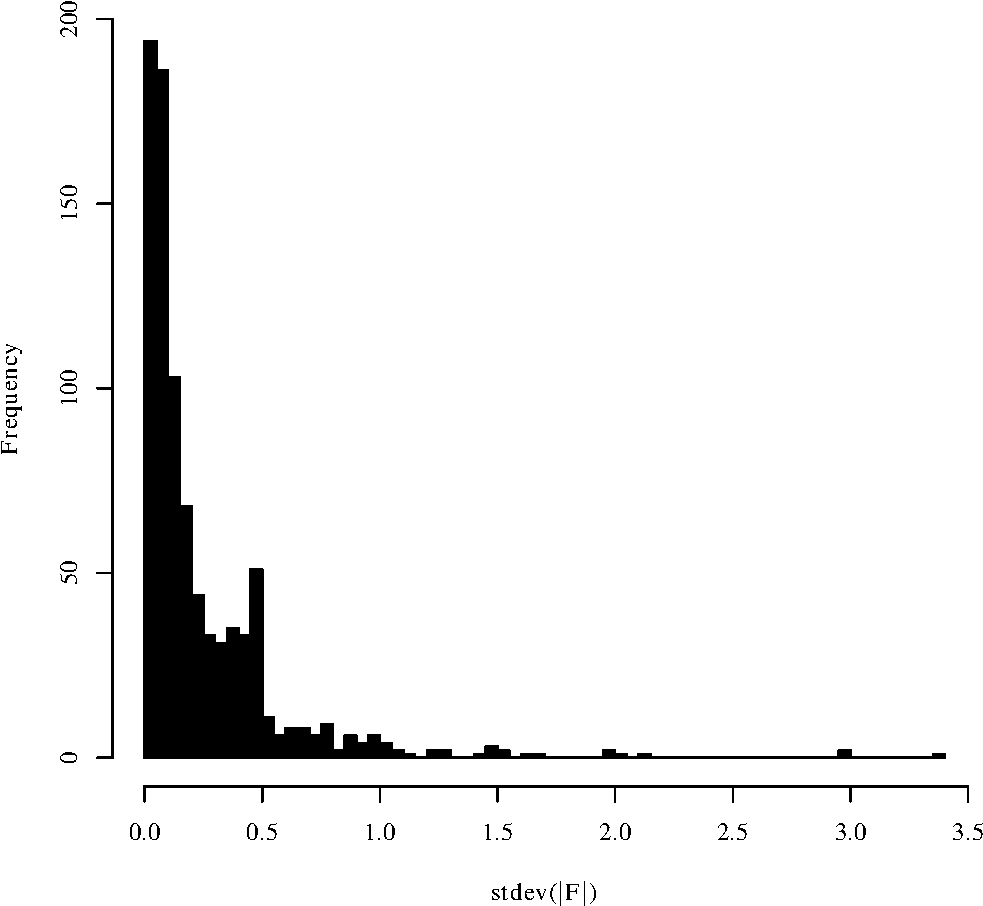
\includegraphics[width=.5\textwidth]{figures/web/conceptdrift/fig_stddev_forms}\label{subfig:website-forms-changes}}
  \subfloat[Avg. time between changes in
  $|F|$.]{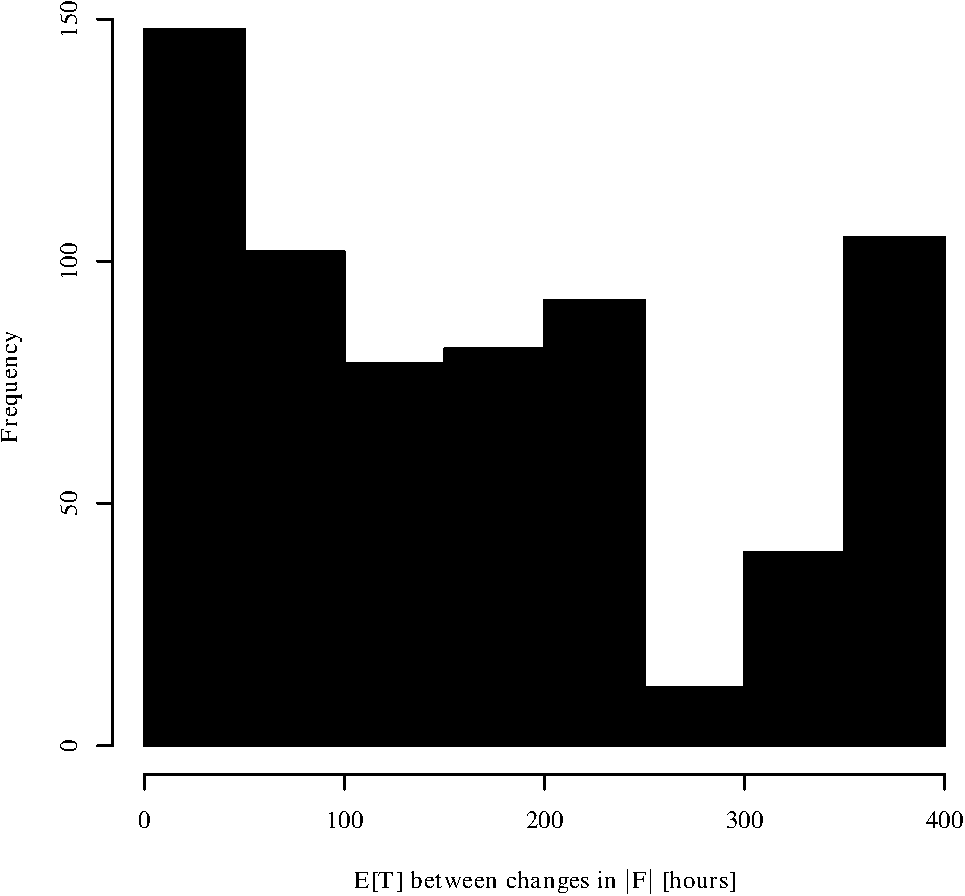
\includegraphics[width=.5\textwidth]{figures/web/conceptdrift/fig_atf}\label{subfig:website-forms-change-time}}\\

  \subfloat[Changes of
  inputs.]{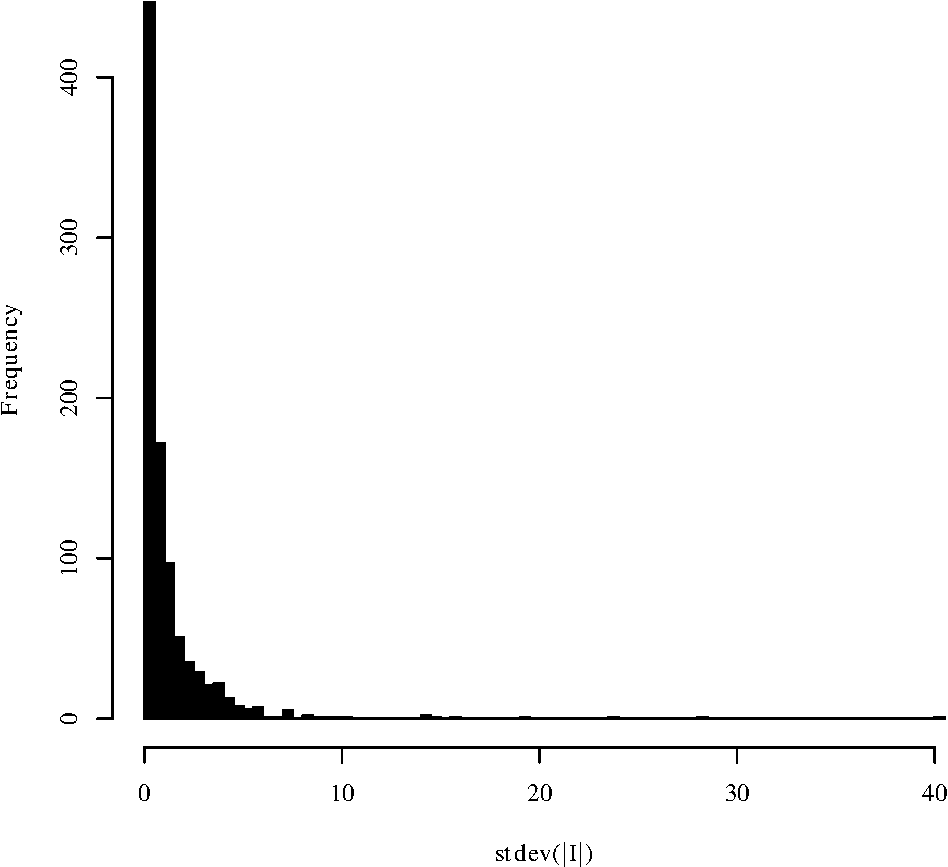
\includegraphics[width=.5\textwidth]{figures/web/conceptdrift/fig_stddev_inputs}\label{subfig:website-inputs-changes}}
  \subfloat[Avg. time between changes in
  $|I|$]{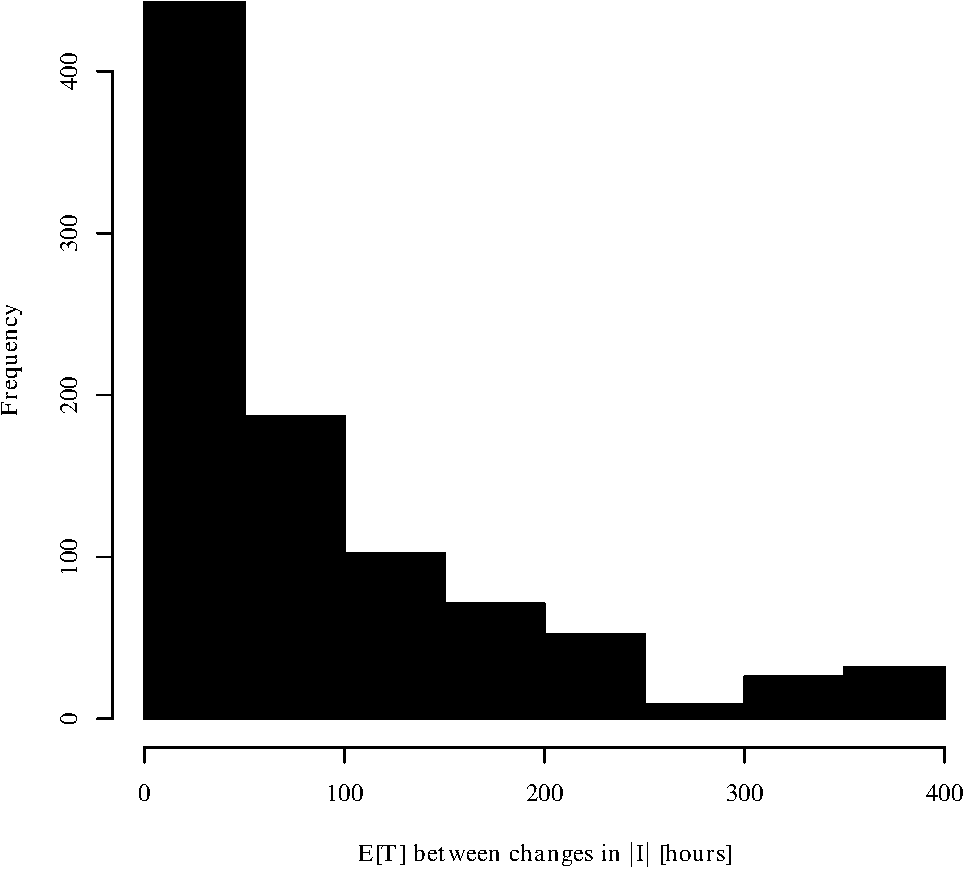
\includegraphics[width=.5\textwidth]{figures/web/conceptdrift/fig_ati}\label{subfig:website-inputs-change-time}}

  \caption{Relative frequency of the standard deviation of the number
    of forms \protect\subref{subfig:website-forms-changes} and input
    fields \protect\subref{subfig:website-inputs-changes}. Also, the
    distribution of the expected time between changes of forms
    \protect\subref{subfig:website-forms-change-time} and input fields
    \protect\subref{subfig:website-inputs-change-time} are plotted. A
    non-negligible portion of the websites exhibits changes in the
    responses. No differences have been noticed between home pages and
    manually-selected pages.}
  \label{fig:website-features-changes}
  \vspace*{-.65cm}
\end{figure}

\paragraph{Second Experiment: Type of Changes}
We monitored in depth three large, data-centric web applications over several months: \textsf{Yahoo!  Mail}, \textsf{YouTube}, and \textsf{MySpace}. We dumped \ac{HTTP}\index{HTTP} responses captured by emulating user interaction using a custom, scriptable web browser implemented with \textsf{Html\hyp{}Unit}. Examples of these interactions are as follows: visit the home page, login, browse the inbox, send messages, return to the home page, click links, log out. Manual inspection revealed some major changes in \textsf{Yahoo! Mail}. For instance, the most evident change consisted of a set of new features added to the search engine (e.g., local search, refined address field in maps search), which manifested themselves as new parameters found in the web search page (e.g. to take into account the country or the ZIP code). User pages of \textsf{YouTube} were significantly updated with new functionalities between 2008 and 2009. For instance, the new version allows users to rearrange widgets in their personal pages. To account for the position of each element, new parameters are added to the profile pages and submitted asynchronously whenever the user drags widgets within the layout. The analysis on \textsf{MySpace} did not reveal any significant change. The results of these two experiments show that changes in server-side applications are common. More importantly, these modifications often involve the way user data is represented, handled, and manipulated.

\paragraph{Third Experiment: Abundance of Code Change}
\label{web:concept-drift:motivation:third}
We analyzed changes in the requests and sessions by inspecting the
code repositories of three of the largest, most popular open-source
web applications: \textsf{WordPress}, \textsf{Movable Type}, and
\textsf{PhpBB}. The goal was to understand whether upgrading a web
application to a newer release results in significant changes in the
features that are used to determine its behavior. In this analysis, we
examined changes in the source code that affect the manipulation of
\ac{HTTP}\index{HTTP} responses, requests, and session data. We used
\textsf{StatSVN}, an open-source tool for tracking and visualizing the
activity of \ac{SVN}\index{SVN} repositories (e.g., the number of
lines changed or the most active developers). We modified
\textsf{StatSVN} to incorporate a set of heuristics to compute
approximate counts of the lines of code that, directly or indirectly,
manipulate \ac{HTTP}\index{HTTP} session, request or response data. In
the case of \ac{PHP}\index{PHP}, examples representative of such lines
include, but are not limited to,
\texttt{\_REQUEST|\_SESSION|\_POST|\_GET|session\_[a-z]+|http\_|strip\_tags|addslashes}. In
order to take into account data manipulation performed through library
functions (e.g., \textsf{WordPress}' custom \texttt{Http} class), we
also generated application-specific code patterns by manually
inspecting and filtering the core
libraries. Figure~\ref{fig:code-changes} shows, over time, the lines
of code in the repositories of \textsf{PhpBB}, \textsf{WordPress}, and
\textsf{Movable Type} that manipulate \ac{HTTP}\index{HTTP} responses,
requests and, sessions. These results show the presence of significant
modifications in the web application in terms of relevant lines of
code added or removed. More importantly, such modifications affect the
way \ac{HTTP}\index{HTTP} data is manipulated and, thus, impact
request, response or session models.

\begin{figure}[p]
  \centering
  \subfloat[\textsf{PhpBB}]{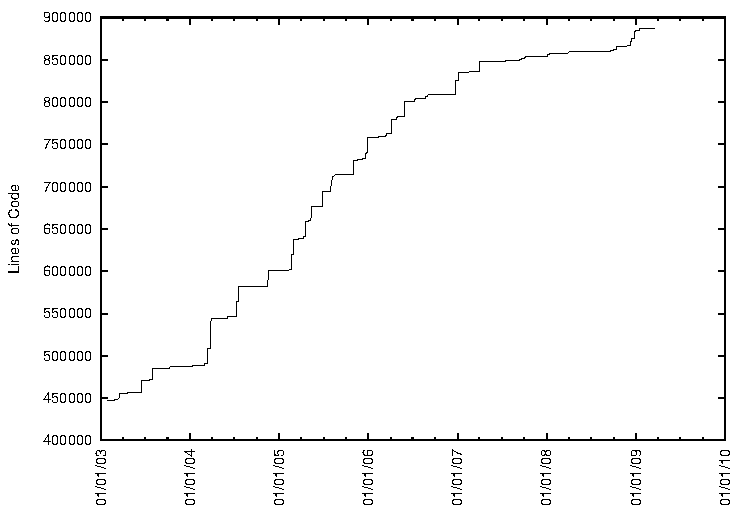
\includegraphics[width=.7\textwidth]{figures/web/conceptdrift/fig_phpbb_svn_loc}\label{subfig:phpbb-code-changes}}\\
  \subfloat[\textsf{WordPress}]{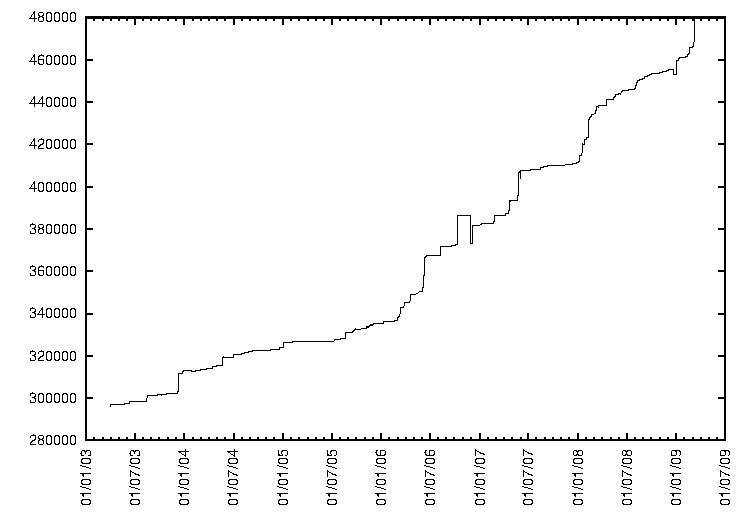
\includegraphics[width=.7\textwidth]{figures/web/conceptdrift/fig_wp_svn_loc}\label{subfig:wordpress-code-changes}}\\
  \subfloat[\textsf{Movable Type}]{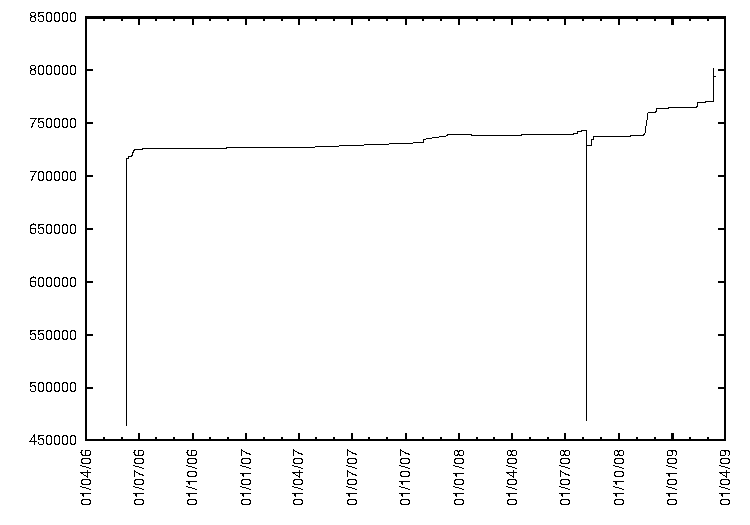
\includegraphics[width=.7\textwidth]{figures/web/conceptdrift/fig_mtos_svn_loc}\label{subfig:movabletype-code-changes}}

  \caption{Lines of codes in the repositories of \textsf{PhpBB}, \textsf{WordPress}, and \textsf{Movable Type}, over time. Counts include only the code that manipulates \ac{HTTP}\index{HTTP} responses, requests and sessions.}
  \label{fig:code-changes}
  \vspace*{-.65cm}
\end{figure}

The aforementioned experiments confirm that the class of changes we described in Section~\ref{web:conceptdrift:motivation:dynamic} is common in real-world web applications. Therefore, anomaly detectors for web applications must incorporate procedures to prevent false alerts due to concept drift. In particular, a mechanism is needed to discriminate between legitimate and malicious changes, and respond accordingly. Note that, this somehow coincides with the original definition of \ac{ID} (i.e., distinguishing among normal \emph{vs.} malicious activity); however, our focus is to recognizes changes in the application \emph{activity} that could lead to concept drift as opposed to spotting out changes in the application \emph{behavior} (i.e., \ac{ID}).

\subsection{Addressing concept drift}
\label{web:conceptdrift:design}
In this section, a technique is presented to distinguish between legitimate changes in web application behavior and evidence of malicious behavior.

\subsubsection{Exploiting HTTP responses}
\label{web:conceptdrift:design:oracle}
An \ac{HTTP}\index{HTTP} response is composed of a header and a body. Under the hypothesis of content-type \texttt{text/html}, the body of \ac{HTTP}\index{HTTP} responses contains a set of links $L_i$ and forms $F_i$ that refer to a set of target resources.  Each form also includes a set of input fields $I_i$.  In addition, each link $l_{i,j}\in L_i$ and form $f_{i,j}\in F_i$ has an associated set of parameters.

A request $q_{i}$ to a resource $r_{i}$ returns a response $resp_{i}$. From $resp_{i}$ the client follows a link $l_{i,j}$ or submits a form $f_{i,j}$.  Either of these actions generates a new \ac{HTTP}\index{HTTP} request to the web application with a set of parameter key-value pairs, resulting in the return of a new \ac{HTTP}\index{HTTP} response to the client, $r_{i+1}$, the body of which contains a set of links $L_{i+1}$ and forms $F_{i+1}$. According to the specifications of the \ac{HTTP}\index{HTTP}, this process continues until the session has ended (i.e., either the user has explicitly logged out, or a timeout has occurred). We then define:

\begin{definition}[Candidate Resource Set]
  Given a resource $r$ within a web application, the \emph{candidate resource set} of $r$ is defined as:

  \begin{eqnarray*}
    \mathrm{candidates(r)} & := & L_{r} \cup F_{r} = \\
                           & = & \{l_{1}, l_{2}, \dots, l_{N}\} \cup\\
                           &    & \{f_{1}, f_{2}, \dots, f_{M}\}.
  \end{eqnarray*}

  \noindent where:

  \begin{itemize}

  \item $l_{(\cdot)} := resp.\mathtt{a_{(\cdot)}.href}$,

  \item $f_{(\cdot)} := resp.\mathtt{form_{\mathrm{(\cdot)}}.action}$,

  \item $resp.$ is the \texttt{plain/text} body of the response $resp$,

  \item $resp.$\texttt{<element>}$_{\mathrm{(\cdot)}}.$\texttt{<attribute>}
    is the content of the attribute,

  \item \texttt{<attribute>}, of the \ac{HTML}\index{HTML}
    \texttt{<element>}$_{(\cdot)}$.
  \end{itemize}
\end{definition}

Our key observation is that, at each step of a web application session, a subset of the \emph{potential} target resources is given exactly by the content of the current resource.  That is, given $r_i$, the associated sets of links $L_i$ and forms $F_i$ directly encode a significant sub-set of the possible $r_{i+1}$.  Furthermore, each link $l_{i,j}$ and form $f_{i,j}$ indicates a precise set of expected parameters and, in some cases, the set of legitimate values for those parameters that can be provided by a client.

Consider a hypothetical banking web application, where the current resource $r_i=\mathtt{/account}$ presented to a client is an account overview. The response $resp_{i}$ may contain:

\begin{html}
<body class="account">
  /* ... */

  <form action="/search" method="get">
    <input name="term" type="text" value="Insert term" />
    <input type="submit" value="Search!" />
  </form>  

  <h1><a href="/account/transfer">Transfer funds</a></h1>
  <a href="/account/transfer/submit">Submit transfer</a>

  /* ... */

  <tr><td><a href="/account/history?aid=328849660322">See details</a></td></tr>
  <tr><td><a href="/account/history?aid=446825759916">See details</a></td></tr>

  /* ... */

  <a href="/logout">Logout</a>

  /* ... */

  <h2>Feedback on this page?</h2>
  <form action="/feedback" method="post" class="feedback-form">
    <select name="subject">
      <option>General</option>
      <option>User interface</option>
      <option>Functionality</option>
    </select>
    <textarea name="message" />
    <input type="submit" />
  </form>

  /* - */
</body>
\end{html}

\noindent containing a set of links $L_{i}$, represented as their \ac{URL}\index{URL}, for instance:

\begin{displaymath}
  L_{i} =
  \left\{
    \begin{array}{l}
      \texttt{/account/history?aid=328849660322},\\
      \texttt{/account/history?aid=446825759916},\\
      \texttt{/account/transfer/submit},\\
      \texttt{/account/transfer},\\
      \texttt{/logout}
    \end{array}
  \right\}.
\end{displaymath}

\noindent Forms are represented as their target action. For instance: $F_{i} =\{$\texttt{/feedback}, \texttt{/search}$\}$.

From $L_i$ and $F_i$, we can deduce the set of legal candidate resources for the next request $r_{i+1}$.  Any other resource would, by definition, be a deviation from a legal session flow through the web application as specified by the application itself.  For instance, it would not be expected behavior for a client to directly access \texttt{/account/transfer/submit} (i.e., a resource intended to submit an account funds transfer) from $r_i$.  Furthermore, for the resource \texttt{/account/history}, it is clear that the web application expects to receive a single parameter \texttt{aid} with an account number as an identifier.

In the case of the form with target \texttt{/feedback}, let the associated input elements be:

\begin{html}
    <select name="subject">
      <option>General</option>
      <option>User interface</option>
      <option>Functionality</option>
    </select>
    <textarea name="message" />
\end{html}

It immediately follows that any invocation of the \texttt{/feedback} resource from $r_i$ should include the parameters \texttt{subject} and \texttt{message}.  In addition, the legal set of values for the parameter \texttt{subject} is given by enumerating the enclosed \texttt{<option~/>} tags. Valid values for the new \texttt{tz} and \texttt{datetime} parameters mentioned in the example of Section~\ref{web:conceptdrift:motivation:dynamic} can be inferred using the same algorithm. Any deviation from these specifications could be considered evidence of malicious behavior.

In this section we described why responses generated by a web application constitute a specification of the intended behavior of clients and the expected inputs to an application's resources.  As a consequence, when a change occurs in the interface presented by a web application, this will be reflected in the content of its responses.  Therefore, as detailed in the following section, an anomaly detection system can take advantage of response modeling to detect and adapt to changes in monitored web applications.

\subsubsection{Adaptive response modeling}
\label{web:conceptdrift:design:responses}
In order to detect changes in web application interfaces, the response modeling of \webanomaly has been augmented with the ability to build $L_{i}$ and $F_{i}$ from the \ac{HTML}\index{HTML} documents returned to a client. The approach is divided into two phases.

\paragraph{Extraction and parsing}
\label{web:conceptdrift:design:responses:extraction-parsing}
The anomaly detector parses each \ac{HTML}\index{HTML} document contained in a response issued by the web application to a client.  For each \texttt{<a~/>} tag encountered, the contents of the \texttt{href} attribute is extracted and analyzed.  The link is decomposed into tokens representing the protocol (e.g., \texttt{http}, \texttt{https}, \texttt{javascript}\index{JavaScript}, \texttt{mailto}), target host, port, path, parameter sequence, and anchor.  Paths are subject to additional processing; for instance, relative paths are normalized to obtain a canonical representation.  This information is stored as part of an abstract document model for later processing.

A similar process occurs for forms.  When a \texttt{<form~/>} tag is encountered, the \texttt{action} attribute is extracted and analyzed as in the case of the link \texttt{href} attribute.  Furthermore, any \texttt{<input~/>}, \texttt{<textarea~/>}, or \texttt{<select~/>} and \texttt{<option~/>} tags enclosed by a particular \texttt{<form~/>} tag are parsed as parameters to the corresponding form invocation.  For \texttt{<input~/>} tags, the \texttt{type}, \texttt{name}, and \texttt{value} attributes are extracted. For \texttt{<textarea~/>} tags, the \texttt{name} attribute is extracted.  Finally, for \texttt{<select~/>} tags, the \texttt{name} attribute is extracted, as well as the content of any enclosed \texttt{<option~/>} tags.  The target of the form and its parameters are recorded in the abstract document model as in the case for links.

\paragraph{Analysis and modeling}
\label{web:conceptdrift:design:responses:analysis-modeling}
The set of links and forms contained in a response is processed by the anomaly engine.  For each link and form, the corresponding target resource is compared to the existing known set of resources.  If the resource has not been observed before, a new model is created for that resource.  The session model is also updated to account for a potential transition from the resource associated with the parsed document and the target resource by training on the observed session request sequence.

For each of the parameters parsed from links or forms contained in a response, a comparison with the existing set of known parameters is performed.  If a parameter has not already been observed (e.g., the new \texttt{tz} parameter), a profile is created and associated with the target resource model.

Any values contained in the response for a given parameter are processed as training samples for the associated models.  In cases where the total set of legal parameter values is specified (e.g., \texttt{<select~/>} and \texttt{<option~/>} tags), the parameter profile is updated to reflect this.  Otherwise, the profile is trained on subsequent requests to the associated resource.

As a result of this analysis, the anomaly detector is able to adapt to changes in session structure resulting from the introduction of new resources.  In addition, the anomaly detector is able to adapt to changes in request structure resulting from the introduction of new parameters and, in a limited sense, to changes in parameter values.

\begin{figure}[t]
  \centering
  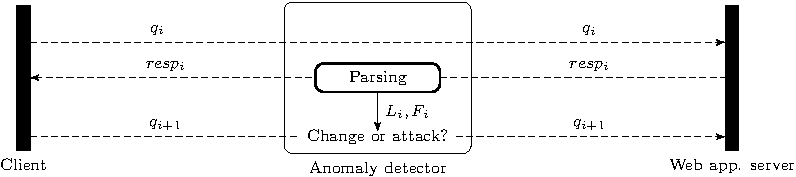
\includegraphics[width=\textwidth]{figures/web/conceptdrift/fig_design}

  \caption{A representation of the interaction between the client and the web application server, monitored by a learning-based anomaly detector. After request $q_{i}$ is processed, the corresponding response $resp_{i}$ is intercepted and link $L_{i}$ and forms $F_{i}$ are parsed to update the request models. This knowledge is exploited as a change detection criterion for the subsequent request $q_{i+1}$.}
  \label{fig:design}
  \vspace*{-.5cm}
\end{figure}

\subsubsection{Advantages and limitations}
\label{web:conceptdrift:design:discussion}
Due to the response modeling algorithm described in the previous section, an anomaly detector is able to automatically adapt to many common changes observed in web applications as modifications are made to the interface presented to clients.  Both changes in session and request structure such as those described in Section~\ref{web:conceptdrift:motivation:dynamic} can be accounted for in an automated fashion.

\begin{example}[I18N and L10N]
  The aforementioned modification is correctly handled as it consists in an addition of the \texttt{tz} parameter and a modification of the \texttt{datetime} parameter.
\end{example}

Furthermore, we claim that web application anomaly detectors that do not perform response modeling cannot reliably distinguish between anomalies caused by legitimate changes in web applications and those caused by malicious behavior.  Therefore, as will be shown in Section~\ref{web:conceptdrift:eval}, any such detector that solely monitors requests is more prone to false positives in the real world.

\medskip

\noindent Clearly, the technique relies upon the assumption that the web application has not been compromised.  Since the web application, and in particular the documents it generates, is treated as an oracle for whether a change has occurred, if an attacker were to compromise the application in order to introduce a malicious change, the malicious behavior would be learned as normal by the detector.  Of course, in this case, the attacker would already have access to the web application. However, modern anomaly detectors like \webanomaly observes all requests and responses to and from untrusted clients, therefore, any attack that would compromise response modeling would be detected and blocked.

\begin{example}
  An attacker could attempt to evade the anomaly detector by introducing a malicious change in the \ac{HTTP}\index{HTTP} responses and then exploits the change detection technique that would interpret the new malicious request as a legit change.

For instance, the attacker could incorporate a link that contain a parameter used to inject the attack vector. To this end, the attacker would have to gain control of the server by leveraging an existing vulnerability of the web application (e.g., a buffer overflow, a \ac{SQL}\index{SQL} injection). However, the \ac{HTTP}\index{HTTP} requests used by the attacker to exploit the vulnerability will trigger several models (e.g., the string length model, in the case of a buffer overflow) and, thus, will be flagged as anomalous\footnote{The threat model assumes that the attacker can interact with the web application only by sending \ac{HTTP}\index{HTTP} requests.}.
\end{example}

In fact, our technique does not alter the ability of the anomaly detector to detect attacks. On the other hand, it avoids many false positives, as demonstrated in Section~\ref{web:conceptdrift:eval:detection}.

Besides the aforementioned assumption, three limitations are important to note.

\begin{itemize}
\item The set of target resources may not always be statically derivable from a given resource. For instance, this can occur when client-side scripts are used to dynamically generate page content, including links and forms.  Accounting for dynamic behavior would require the inclusion of script interpretation.  This, however, has a high overhead, is complex to perform accurately, and introduces the potential for denial of service attacks against the anomaly detection system.  For these reasons, such a component is not implemented in the current version of \webanomaly, although further research is planned to deal with dynamic behavior.

\item The technique does not fully address changes in the behavior of individual request parameters in its current form.  In cases where legitimate parameter values are statically encoded as part of an \ac{HTML}\index{HTML} document, response modeling can directly account for changes in the legal set of parameter values.  Unfortunately, in the absence of any other discernible changes in the response, changes in parameter values provided by clients cannot be detected. However, heuristics such as detecting when all clients switch to a new observable behavior in parameter values (i.e., all clients generate anomalies against a set of models in a similar way) could serve as an indication that a change in legitimate parameter behavior has occurred.

\item The technique cannot handle the case where a resource is the result of a parametrized query and the previous response has not been observed by the anomaly detector.  In our experience, however, this does not occur frequently in practice, especially for sensitive resources.
\end{itemize}

\subsection{Experimental Results}
\label{web:conceptdrift:eval}
In this section, we show that our techniques reliably distinguish between legitimate changes and evidence of malicious behavior, and present the resulting improvement in terms of detection accuracy.

The goal of this evaluation is twofold. We first show that concept drift in modeled behavior caused by changes in web applications results in lower detection accuracy. Second, we demonstrate that our technique based on \ac{HTTP}\index{HTTP} responses effectively mitigates the effects of concept drift. To this end, we adopted the training dataset described in Section~\ref{web:intro:eval}.

\subsubsection{Effects of concept drift}
\label{web:conceptdrift:eval:effects}
In the first experiment, we demonstrate that concept drift as observed in real-world web applications results in a significant negative impact on false positive rates.

\begin{enumerate}
\item \webanomaly was trained on an unmodified, filtered data set.  Then, the detector analyzed a test data set $Q$ to obtain a baseline \ac{ROC}\index{ROC} curve.

\item After the baseline curve had been obtained, the test data set was processed to introduce new behaviors corresponding to the effects of web application changes, such as upgrades or source code refactoring, obtaining $Q_{\text{drift}}$.  In this manner, the set of changes in web application behavior was explicitly known.  In particular, as detailed in Table~\ref{fig:fpr-table}:

\begin{description}
  \item [sessions] 6,749 new session flows were created by introducing requests for new resources and creating request sequences for both new and known resources that had not previously been observed;
  \item [parameters] new parameter sets were created by introducing 6,750 new parameters to existing requests;
  \item [values] the behavior of modeled features of parameter values was changed by introducing 5,785 mutations of observed values in client requests.
\end{description}

\noindent For example, each sequence of resources

\begin{displaymath}
  \langle\texttt{/login, /index, /article}\rangle
\end{displaymath}

might be transformed to

\begin{displaymath}
  \langle\texttt{/login, /article}\rangle.
\end{displaymath}

\noindent Similarly, each request like \texttt{/categories} found in the traffic might be replaced with \texttt{/foobar}.  For new parameters, a set of link or form parameters might be updated by changing a parameter name and updating requests accordingly.

It must be noted that in all cases, responses generated by the web application were modified to reflect changes in client behavior.  To this end, references to new resources were inserted in documents generated by the web application, and both links and forms contained in documents were updated to reflect new parameters.

\item \webanomaly -- without the \ac{HTTP}\index{HTTP} response modeling technique enabled -- was then run over $Q_{\text{drift}}$ to determine the effects of concept drift upon detector accuracy.
\end{enumerate}

The resulting \ac{ROC}\index{ROC} curves are shown in Figure~\ref{fig:changes-increase-fpr}.  The consequences of web application change are clearly reflected in the increase in false positive rate for $Q_{\text{drift}}$ versus that for $Q$.  Each new session flow and parameter manifests as an alert, since the detector is unable to distinguish between anomalies due to malicious behavior and those due to legitimate change in the web application.

\begin{figure}[t]
  \centering
  \subfloat[Response modeling disabled.]{
    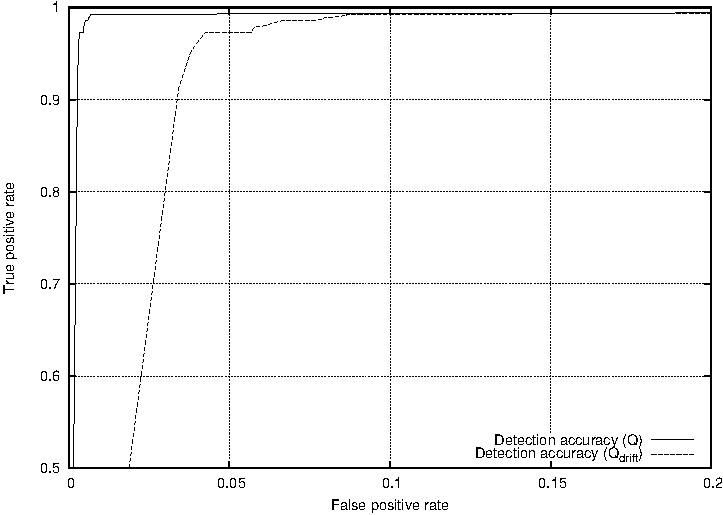
\includegraphics[width=0.48\textwidth]{figures/web/conceptdrift/fig_alerts}
    \label{fig:changes-increase-fpr}}
  \subfloat[Response modeling enabled.]{
    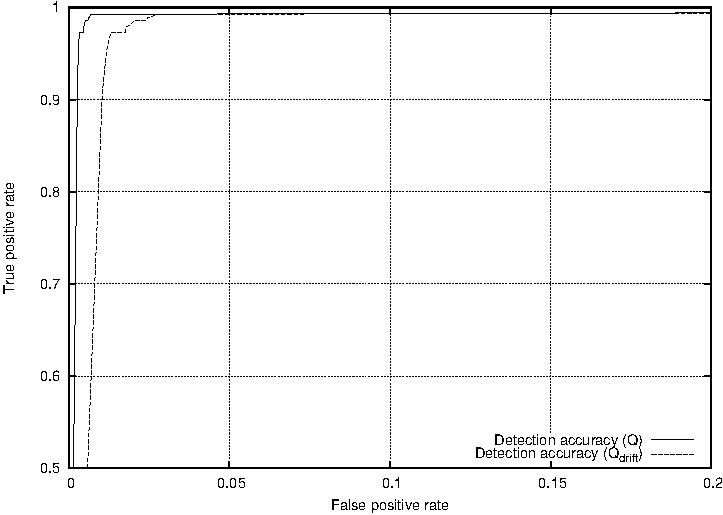
\includegraphics[width=0.48\textwidth]{figures/web/conceptdrift/fig_alerts_resp}
    \label{fig:response-models-fpr}}

  \caption{Detection and false positive rates measured on $Q$ and $Q_{\text{drift}}$, with \ac{HTTP}\index{HTTP} response modeling enabled in (b).}
\end{figure}

\subsubsection{Change detection}
\label{web:conceptdrift:eval:detection}
The second experiment quantifies the improvement in the detection accuracy of \webanomaly in the presence of web application change.  As before, the detector was trained over an unmodified filtered data set, and the resulting profiles were evaluated over both $Q$ and $Q_{\text{drift}}$.  In this experiment, however, the \ac{HTTP}\index{HTTP} response modeling technique was enabled.

Figure~\ref{fig:response-models-fpr} presents the results of analyzing \ac{HTTP}\index{HTTP} responses on detection accuracy.  Since many changes in the behavior of the web application and its clients can be discovered using our response modeling technique, the false positive rate for $Q_{\text{drift}}$ is greatly reduced over that shown in Figure~\ref{fig:changes-increase-fpr}, and approaches that of $Q$, where no changes have been introduced.  The small observed increase in false positive rate can be attributed to the effects of changes in parameter values.  This occurs because a change has been introduced into a parameter value submitted by a client to the web application, and no indication of this change was detected on the preceding document returned to the client (e.g., because no \texttt{<select />} were found).

Table~\ref{fig:fpr-table} displays the individual contributions to the reduction of the false positive rate due to the response modeling technique.  Specifically, the total number of anomalies caused by each type of change, the number of anomalies erroneously reported as alerts, and the corresponding reduction in the false positive rate is shown.  The results displayed were generated from a run using the optimal operating point (0.00144, 0.97263) indicated by the knee of the \ac{ROC}\index{ROC} curve in Figure~\ref{fig:response-models-fpr}.  For changes in session flows and parameters sets, the detector was able to identify an anomaly as being caused by a change in web application behavior in all cases.  This resulted in a large net decrease in the false positive rate of the detector with response modeling enabled.  The modification of parameters is more problematic, though; as discussed in Section~\ref{web:conceptdrift:design:discussion}, it is not always apparent that a change has occurred when that change is limited to the type of behavior a parameter's value exhibits.

\begin{table}[t]
  \centering
  \begin{tabular}{rccc}
    \toprule
    \textsc{Change type} & \textsc{Anomalies} & \textsc{FP} & \textsc{Reduction} \\
    \midrule
    New session flows & 6,749 & 0 & 100.0\% \\
    New parameters & 6,750 & 0 & 100.0\% \\
    Modified parameters & 5,785 & 4,821 & 16.6\% \\
    \cmidrule{2-4}
    \emph{Total} & 19,284 & 4,821 & 75.0\% \\
    \bottomrule
  \end{tabular}

  \caption{Reduction in the false positive rate due to \ac{HTTP}\index{HTTP} response modeling for various types of changes.}
  \label{fig:fpr-table}
  \vspace*{-.65cm}
\end{table}

From the overall improvement in false positive rates, we conclude that \ac{HTTP}\index{HTTP} response modeling is an effective technique for distinguishing between anomalies due to legitimate changes in web applications and those caused by malicious behavior.  Furthermore, any anomaly detector that does not do so is prone to generating a large number of false positives when changes do occur in the modeled application.  Finally, as it has been shown in Section~\ref{web:conceptdrift:motivation}, web applications exhibit significant long-term change in practice, and, therefore, concept drift is a critical aspect of web application anomaly detection that must be addressed.

\section{Concluding Remarks}
\label{web:conclusions}
In this chapter we described in detail two approaches to mitigate training issues. In particular, we presented a technique to reduce \acp{FP}\index{FP} due to scarce training data and a mechanism to automatically recognize changes in the monitored applications, such as code updates, and re-train the models without any human intervention.

First, we have described our efforts to cope with an issue that must be addressed by web application anomaly detection systems in order to provide a reasonable level of security.  The impact of this issue is particularly relevant for commercial web-based anomaly detection systems and web application firewall, which have to operate in real-world environment where sufficient training data might be unavailable within a reasonable time frame.

We have proposed the use of global knowledge bases of well-trained, stable profiles to remediate a local scarcity of training data by exploiting global similarities in web application parameters. We found that although using global profiles does result in a small reduction in detection accuracy, the resulting system, when given appropriate parameters, does provide reasonably precise modeling of otherwise unprotected web application parameters.

A possible future extension of the described approach is to investigate the use of other types of models, particularly \ac{HTTP}\index{HTTP} response and session models. An additional line of future work is the application of different clustering methods in order to improve the efficiency of the querying procedure for high-cardinality knowledge bases.

Secondly, we have identified the natural dynamicity of web applications as an issue that must be addressed by modern anomaly-based web application anomaly detectors in order to prevent increases in the false positive rate whenever the monitored web application is changed. We named this frequent phenomenon the \emph{web application concept drift}.

In \citep{2009_maggi_robertson_kruegel_vigna} we proposed the use of novel \ac{HTTP}\index{HTTP} response modeling techniques to discriminate between legitimate changes and anomalous behaviors in web applications. More precisely, responses are analyzed to find new and previously unmodeled parameters. This information is extracted from anchors and forms elements, and then leveraged to update request and session models. We have evaluated the effectiveness of our approach over an extensive real-world data set of web application traffic. The results show that the resulting system can detect anomalies and avoid false alerts in the presence of concept drift.

We plan to investigate the potential benefits of modeling the behavior of JavaScript\index{JavaScript} code, which is becoming increasingly prevalent in modern web applications. Also, additional, richer, and media-dependent response models must be studied to account for interactive client-side components, such as Adobe Flash and Microsoft Silverlight\index{Silverlight} applications.

%%% Local Variables: 
%%% mode: latex
%%% TeX-master: "thesis"
%%% End: 

\chapter{Network and Host Alert Correlation}
\label{correlation}
Either as part of an \ac{IDS} or as a post-processing step, the alert
correlation task is meant to recognize relations among alerts. For
instance, a simple correlation task is to suppress all the alerts
regarding unsuccessful attacks. A more complex example envisions a
large enterprise network monitored by multiple \acp{IDS}, both
host\hyp{} and network\hyp{}based. Whenever a misbehaving application
is detected on a certain machine, the \ac{HIDS} interacts with the
\ac{NIDS} that is monitoring the network segment of that machine to,
say, validate the actual detection result. A more formal definition of
alert correlation and alert correlation systems can be found in
Section~\ref{detection:id:alert-correlation}.

In this section we focus on practical aspects of alert correlation by
first presenting the model we used in our prototype tools. Based on
this model we concentrate on two challenging phases, namely
\emph{aggregation}, which has to do with grouping similar alerts
together, and \emph{correlation}, which is the actual correlation
phase. In particular, in Section~\ref{correlation:fusion} we
investigate the use of fuzzy metrics to time-based aggregation, which
has been proposed recently as a simple but effective aggregation
criterion. Unfortunately, given a threshold of, say, $10s$, this
approach will fail if two alerts are at, say, $10.09s$ to each
other. In Section~\ref{correlation:causality} we focus on the actual
correlation task. We exploit non\hyp{}parametric statistical tests to
create a simple but robust correlation system that is capable of
recognizing series of related events without relying on previous
knowledge. Last, in Section~\ref{correlation:evaluation} we propose a
methodology to compare alert correlation systems which are as
difficult as \acp{IDS} to evaluate.

\section{Fuzzy Models and Measures for Alert Fusion}
\label{correlation:fusion}
In this section we focus on the aggregation of \ac{IDS}\index{IDS}
alerts, an important component of the alert correlation process as
shown on Figure~\ref{fig:correlation_model}. We describe our approach
\citep{2009_maggi_zanero_matteucci_fusion}, which exploit fuzzy
measures and fuzzy sets to design simple and robust alert aggregation
algorithms. Exploiting fuzzy sets, we are able to robustly state
whether or not two alerts are ``close in time'', dealing with noisy
and delayed detections. A performance metric for the evaluation of
fusion systems is also proposed. Finally, we evaluate the fusion
method with alert streams from anomaly-based \ac{IDS}\index{IDS}.

\begin{figure}[t]
  \centering
  \begin{tikzpicture}[node distance=7.5em,every node/.style={inner sep=.5em,font=\footnotesize}]
    \node [draw,shape=rectangle,double copy shadow,fill=white] (ids) {IDS};
    \node (A) [right of=ids,text width=1.2em] {$\mathbb{A}_{1}$\\...\\$\mathbb{A}_{n}$};
    \node [draw,shape=rectangle] (N) [right of=A] {Normalization};
    \node [draw,shape=rectangle] (P) [right of=N] {Prioritization};
    \node [draw,shape=rectangle] (Ag) [below of=P] {Aggregation};
    \node [draw,shape=rectangle] (C) [left of=Ag] {Correlation};
    \node [draw,shape=rectangle] (V) [left of=C] {Verification};
    \node (As) [left of=V] {$\mathbb{A}'$};
    
    \draw[-stealth] (ids) -- (A);
    \draw[-stealth] (A) -- (N);
    \draw[-stealth] (N) -- (P);
    \draw[-stealth] (P) -- (Ag);
    \draw[-stealth] (Ag) -- (C);
    \draw[-stealth] (C) -- (V);
    \draw[-stealth] (V) -- (As);
  \end{tikzpicture}
  \caption{Simplified version of the correlation approach proposed
    in~\citep{valeur04comprehensive}.}
  \label{fig:correlation_model}
\end{figure}

Alert aggregation becomes more complex when taking into account
\emph{anomaly detection} systems, because no information on the type
or classification of the observed attack is available to any of the
fusion algorithms. Most of the algorithms proposed in the current
literature on correlation make use of the information regarding the
matching attack provided by misuse detectors; therefore, such methods
are inapplicable to purely anomaly based intrusion detection
systems. Although some approaches, e.g.,~\citep{1224380}, incorporate
techniques to correlate automatically-generated signatures, such
techniques are aimed at creating more general signatures in order to
augment the DR. Instead, our focus is that of reducing the FPR by
fusing more information sources. However, as described in
Section~\ref{detection:id}, since anomaly and misuse detection are
symmetric, it is reasonable and noteworthy to try to integrate
different approaches through an alert fusion process.

Toward such goal, we explore the use of fuzzy measures
\citep{fuzzymeasure} and fuzzy sets \citep{folger_klir} to design
simple, but robust aggregation algorithms. In particular, we
contribute to one of the key issues, that is how to state whether or
not two alerts are ``close in time''. In addition, uncertainties on
both timestamp measurements and threshold setting make this process
even more difficult; the use of fuzzy sets allows us to precisely
define a time-distance criterion which ``embeds'' unavoidable errors
(e.g., delayed detections).

\subsection{Time-based alert correlation}
\label{correlation:fusion:time-based-alert}
As proposed in most of the reviewed literature, a first, naive
approach consists in exploiting the \emph{time distance} between
alerts for aggregation; the idea is to aggregate ``near'' alerts. In
this section we focus on this point, starting by the definition of
``near''.

Time-distance aggregation might be able to catch simple scenarios like
remote attacks against remote applications vulnerabilities (e.g., web
servers ). For instance, consider the scenario where, at time $t_{0}$,
an attacker violates a host by exploiting a vulnerability of a server
application. An \ac{IDS}\index{IDS} monitoring the system recognizes
anomalous activity at time $t_{n} = t_{0} + \tau_{n}$. Meanwhile, the
attacker might escalate privileges and break through another
application; the \ac{IDS}\index{IDS} would detects another anomaly at
$t_{h} = t_{0} + \tau_{h}$. In the most general case $t_{n}$ is
``close'' to $t_{h}$ (with $t_{n} < t_{h}$), so if $t_{h} - t_{n} \leq
T_{near}$ the two alerts belong to the same attack.

\begin{figure}[p]
  \centering
  
  \subfloat[][]{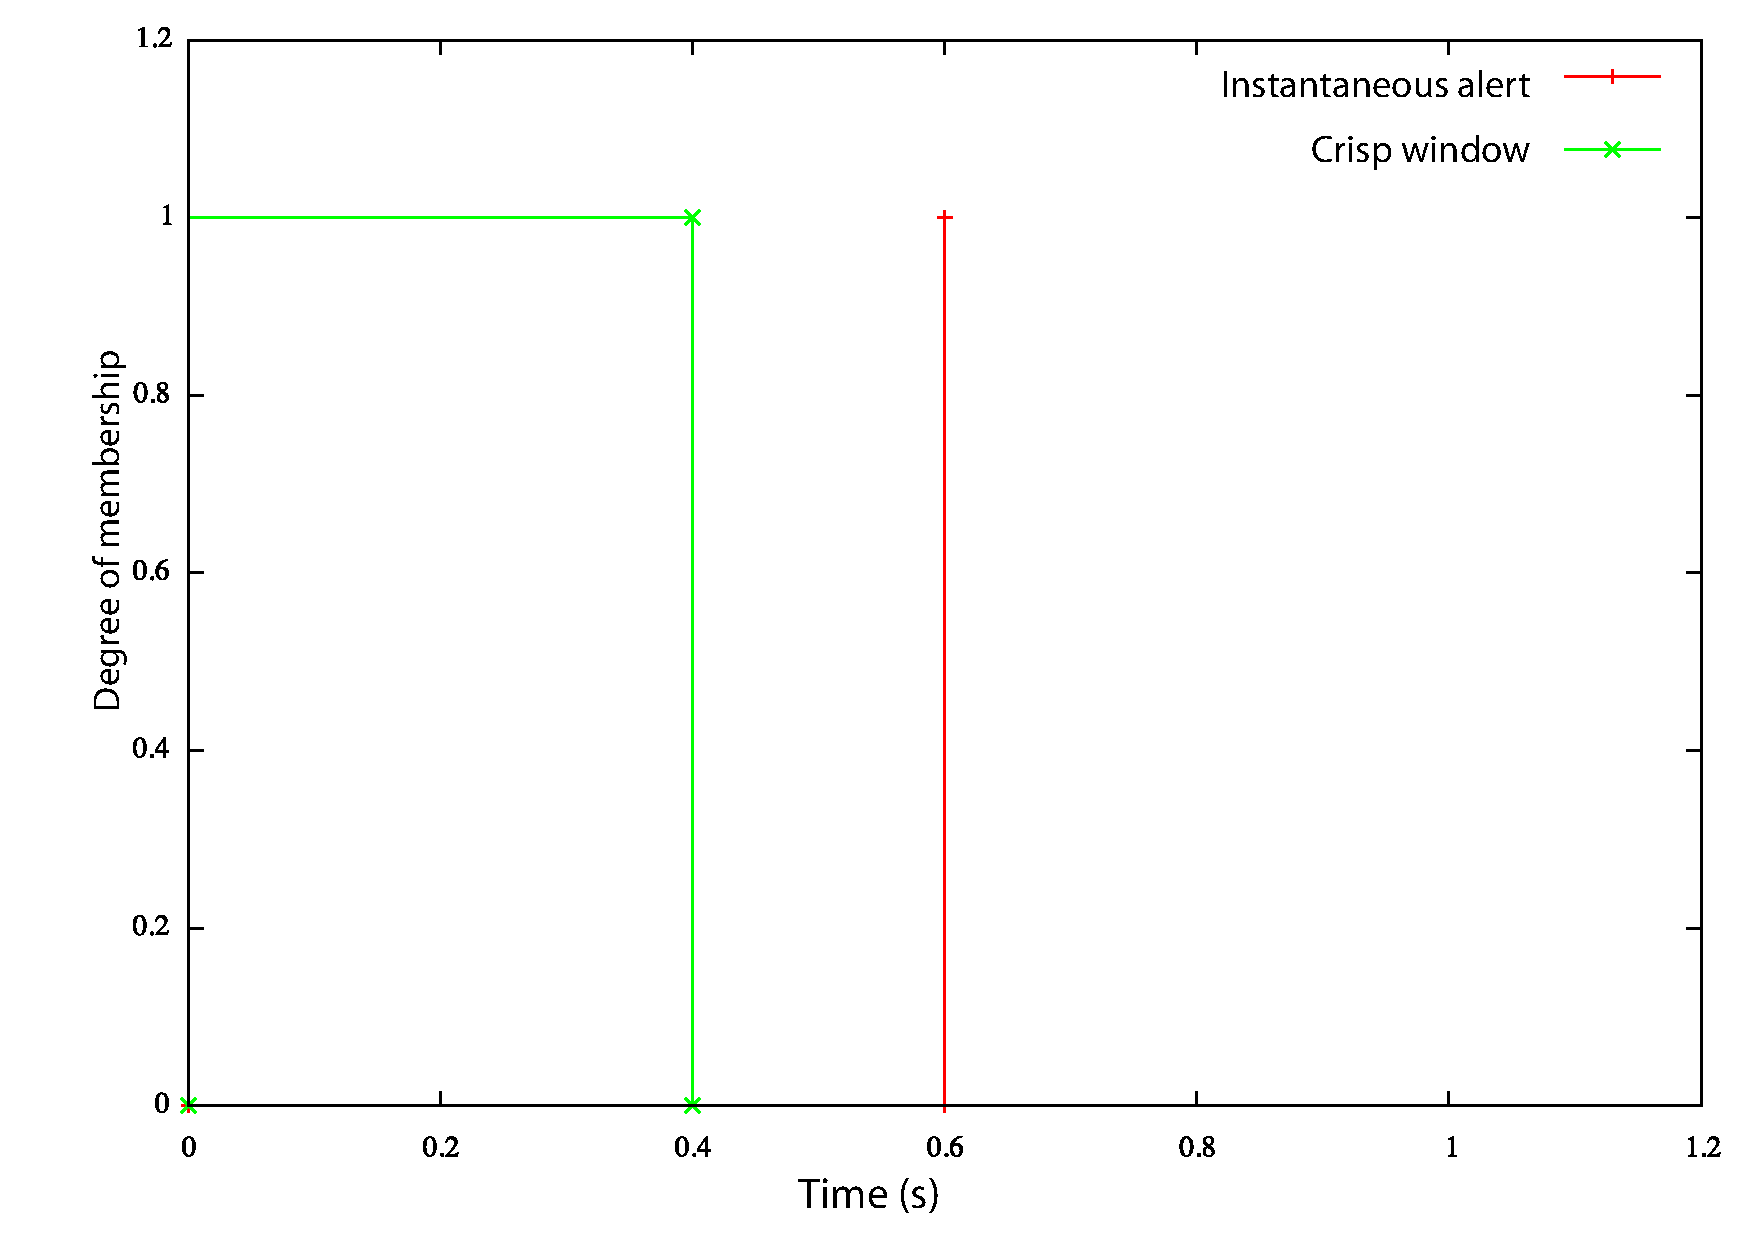
\includegraphics[width=.8\textwidth]{figures/correlation/fusion/fuzzy_crisp_distance}}

  \subfloat[][]{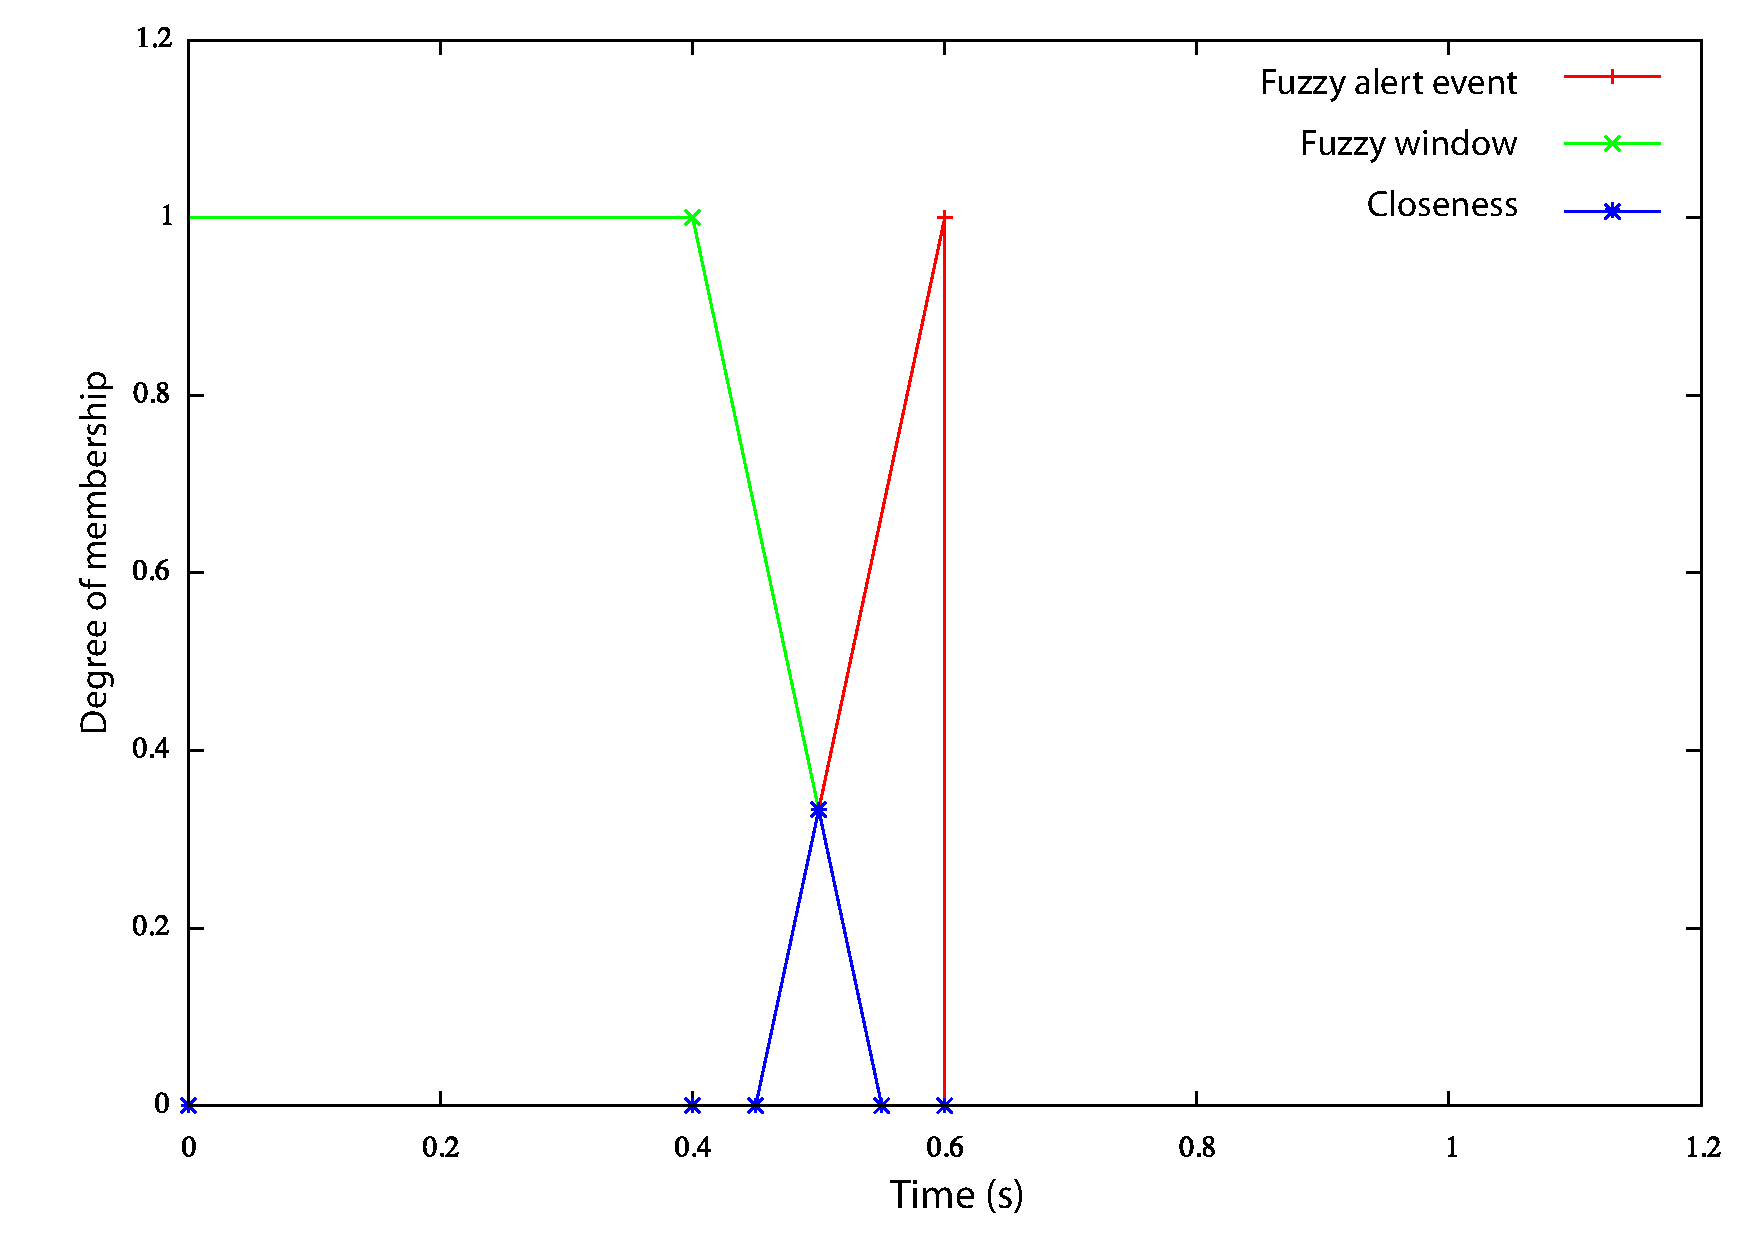
\includegraphics[width=.8\textwidth]{figures/correlation/fusion/fuzzy_distance}}
  
  \caption{Comparison of crisp (a) and fuzzy (b) time-windows. In both
    graphs, one alert is fired at $t = 0$ and another alert occurs at
    $t = 0.6$. Using a crisp time-window and instantaneous alerts (a),
    the distance measurement is not robust to neither delays nor
    erroneous settings of the time-window size. Using fuzzy-shaped
    functions (b) provides more robustness and allows to capture the
    concept of ``closeness'', as implemented with the \textsf{T}-norm
    depicted in (b). Distances in time are normalized in [0,1]
    (w.r.t. the origin).}
  \label{fig:crisp_fuzzy_distance}
\end{figure}

The idea is to \emph{fuse} alerts if they are both close in time, raised from the same \ac{IDS}\index{IDS}, and refer to the same source and destination. This intuition obviously needs to be detailed. First, the concept of ``near'' is not precisely defined; secondly, errors in timestamping are not taken into account; and, a crisp time distance measure is not robust. For instance, if $|t_{h} - t_{n}| = 2.451$ and $T_{near} = 2.450$ the two alerts are obviously near, but not aggregated, because the above condition is not satisfied. To overcome such limitations, we propose a \emph{fuzzy} approach to time-based aggregation.

In the following, we will use the well-known dot notation, as in object-oriented programming languages, to access a specific alert attribute: e.g., $a.start\_ts$ indicates the value of the attribute $start\_ts$ of the alert $a$. Moreover, we will use $T_{(\cdot)}$ to indicate a threshold variable: for instance, $T_{near}$ is the threshold variable called (or regarding to) ``near''.

We rely on fuzzy sets for modeling both the uncertainty on the timestamps of alerts and the time distance in a robust manner. Regarding the uncertainty on measurements, we focus on delayed detections by using triangle-shaped fuzzy sets to model the occurrence of an alert. Since the measured timestamp may be affected by errors or delays, we extend the singleton shown in Figure \ref{fig:crisp_fuzzy_distance} (a) with a triangle, as depicted in Figure \ref{fig:crisp_fuzzy_distance} (b). We also take into account uncertainty on the dimension of the aggregation window: instead of using a crisp window (as in Figure \ref{fig:crisp_fuzzy_distance} (a)), we extend it to a trapezoidal fuzzy set, resulting in a more robust distance measurement. In both graphs, one alert is fired at $t = 0$ and another alert occurs at $t = 0.6$. Using a crisp time-window and instantaneous alerts (Figure \ref{fig:crisp_fuzzy_distance} (a)), the distance measurement is not robust to neither delays nor erroneous settings of the time-window size. Using fuzzy-shaped functions (Figure \ref{fig:crisp_fuzzy_distance} (b)) provides more robustness and allows to capture the concept of ``closeness'', as implemented with the \textsf{T}-norm depicted in Figure \ref{fig:crisp_fuzzy_distance} (b). In Figure \ref{fig:crisp_fuzzy_distance} distances in time are normalized in [0,1] (w.r.t. the origin).

Note that, Figure \ref{fig:fuzzy_delay} compares two possible manners to model uncertainty on alert timestamps: in Figure \ref{fig:fuzzy_delay} (a) the alert is recorded at 0.5 seconds but the measurement may have both positive (in the future) and negative (in the past) errors. Figure \ref{fig:fuzzy_delay} (b) is more realistic because positive errors are not likely to happen (i.e., we cannot ``anticipate'' detections), while events are often delayed, especially in network environments. In comparison to our proposal of using ``fuzzy timestamps'', the \ac{IDMEF} describes event occurrences using \emph{three} timestamps (\texttt{Create-}, \texttt{Detect-}, and \texttt{Analyzer-Time}): this is obviously more generic and allows the reconstruction of the entire event path from the attack to the analyzer that reports the alert. However, all timestamps are not always known: for example, the \ac{IDS} might not have such a feature, thus the \ac{IDMEF} \texttt{Alert}s cannot be completely filled.

\begin{figure}[p]
  \centering
  \subfloat[][]{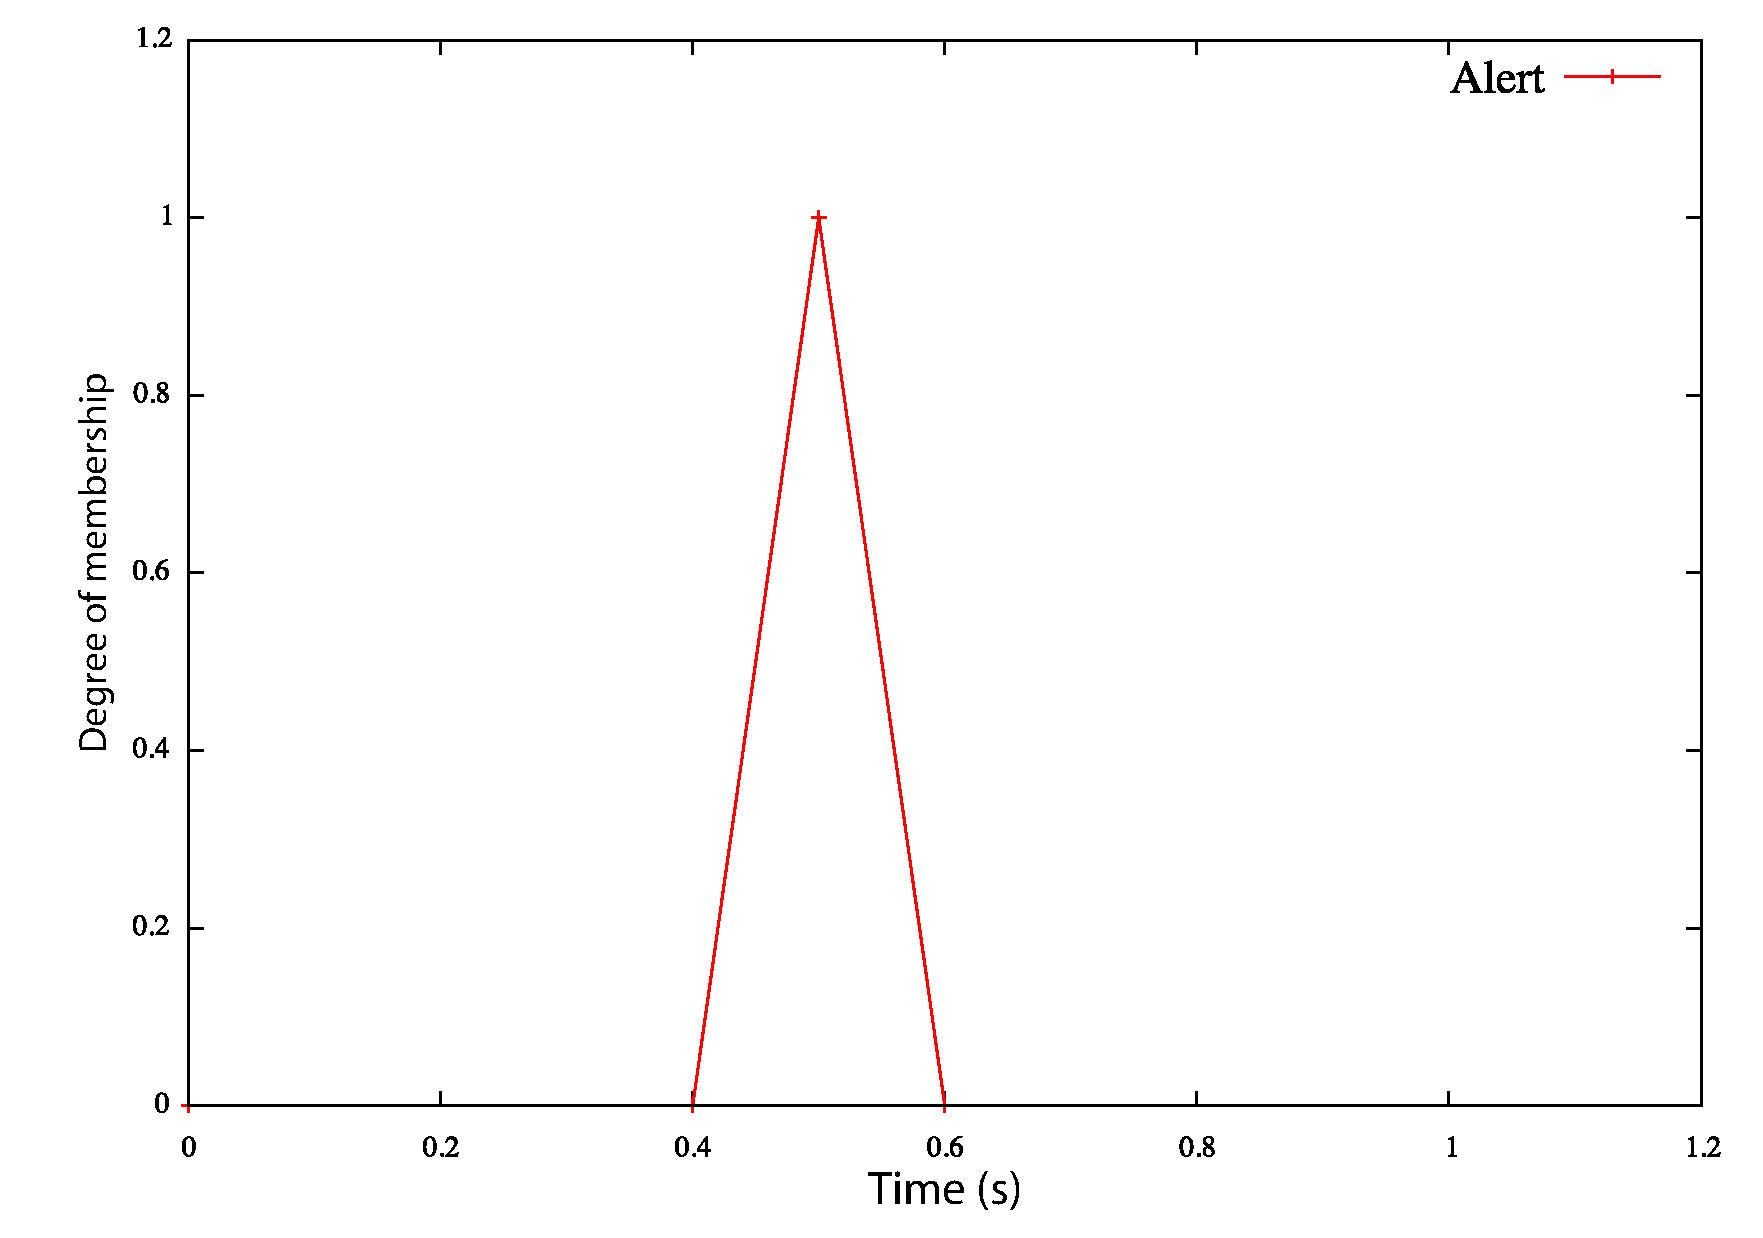
\includegraphics[width=0.8\textwidth]{figures/correlation/fusion/fuzzy_alert_delay}
  }\\

  \subfloat[][]{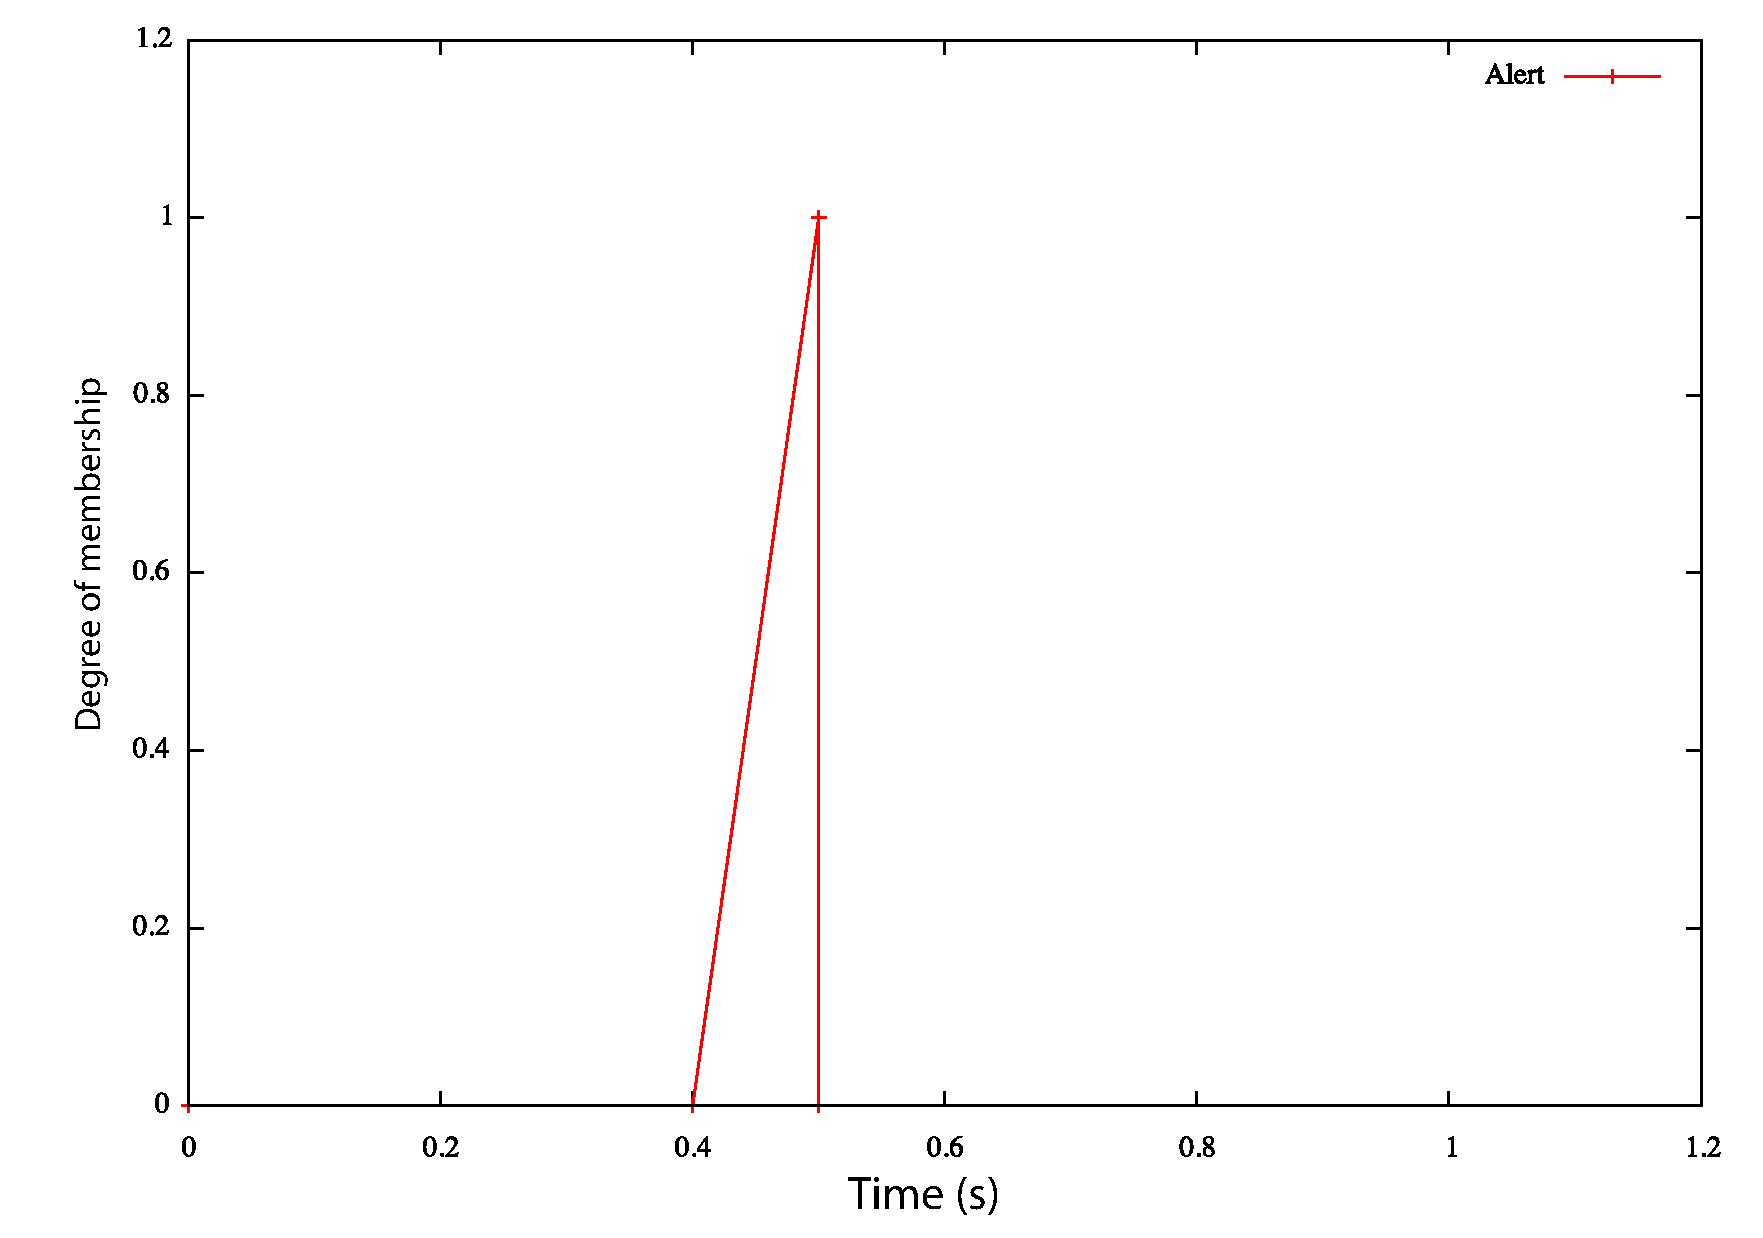
\includegraphics[width=0.8\textwidth]{figures/correlation/fusion/fuzzy_alert_delay_ok}}
  
  \caption{Comparing two possible models of uncertainty on timestamps of single alerts.}
  \label{fig:fuzzy_delay}
\end{figure}

As stated above, the main goal is to measure the time distance between two alerts, $a_{1}$ and $a_{2}$ (note that, in the following, $a_{2}$ occurs after $a_{1}$). We first exemplify the case of instantaneous alerts, that is $a_{i}.start\_ts = a_{i}.end\_ts = a_{i}.ts$ for $i \in \{1, 2\}$. To state whether or not $a_{1}$ is close to $a_{2}$ we use a $T_{near}$ sized time window: in other words, an interval spreading from $a_{1}.ts$ to $a_{1}.ts + T_{near}$ (Figure \ref{fig:crisp_fuzzy_distance} (a) shows the described situation for $a_{1}.ts = 0$, $T_{near} = 0.4$, and $a_{2}.ts = 0.6$: values have been normalized to place $a_{1}$ alert in the origin).

Extending the example shown in Figure \ref{fig:crisp_fuzzy_distance} (a) to uncertainty in measurements is straightforward; let us suppose to have an average uncertainty of 0.15 seconds on the measured (normalized w.r.t. the origin) value of $a_{2}.ts$: we model is as a triangle-shaped fuzzy set as the one drawn in Figure \ref{fig:crisp_fuzzy_distance} (b).

In the second place, our method takes into account uncertainty regarding the thresholding of the distance between two events, modeled in Figure \ref{fig:crisp_fuzzy_distance} (b) by the trapezoidal fuzzy window: the smoothing factor, 0.15 seconds, represents potential errors (i.e., the time values for which the membership function is neither 1 nor 0). Given these premises, the fuzzy variable ``near'' is defined by a T-norm \citep{folger_klir} as shown in Figure \ref{fig:crisp_fuzzy_distance} (b): the resulting triangle represents the alerts overlapping in time. In the example we used $\mathrm{min}(\cdot)$ as T-norm.

In the above examples, simple triangles and trapezoids have been used
but more accurate/complex membership functions could be used as
well. However, we remark here that trapezoid-like sets are
conceptually different from triangles as the former have a membership
value of 100\%; this means certainty on the observed/measured
phenomenon (i.e., closeness), while lower values mean
uncertainty. Trapezoids-like functions should be used whenever a
100\%-certainty interval is known: for instance, in Figure
\ref{fig:crisp_fuzzy_distance} (b) if two alerts occur within 0.4
seconds they are near at 100\%; between 0.4 and 0.55 seconds, such
certainty decreases accordingly.

\begin{note}[Extended crisp window]
  It is important to underline that, from a purely practical point of
  view, one may achieve the same effect on alert fusion by building a
  more ``flexible'' crisp time window (e.g., by increasing its size
  by, say, 15\%). However, from a theoretical point of view, it must
  be noted that our approach explicitly models the errors that occur
  during the alert generation process. On the other hand, by
  increasing a time window of a certain percentage would only give
  more flexibility, without giving any semantic definition of ``near
  alerts''. There is a profound difference between saying ``15\%
  larger'' and assigning a precise membership function to a certain
  variable and defining T-norms for aggregation.
\end{note}

The approach can be easily generalized to take into account
non\hyp{}instantaneous events, i.e. $a_{i}.start\_ts <
a_{i}.end\_ts$. In this case, alerts delays have to be represented by
a trapezoidal fuzzy set. Note that, smoothing parameters are
configurable values as well as fuzzy set shapes, in order to be as
generic as possible w.r.t. the particular network environment; in the
most general case, such parameters should be estimated before the
system deployment. In Figure \ref{fig:fuzzy_alert_trapez} the measured
value of $a_{i}.start\_ts$ is $0.4$, while $a_{i}.end\_ts = 0.8$;
moreover, a smoothing factor of 0.15 seconds is added as a negative
error, allowing the real $a_{i}.start\_ts$ to be 0.25.

\begin{figure}[t]
  \centering
  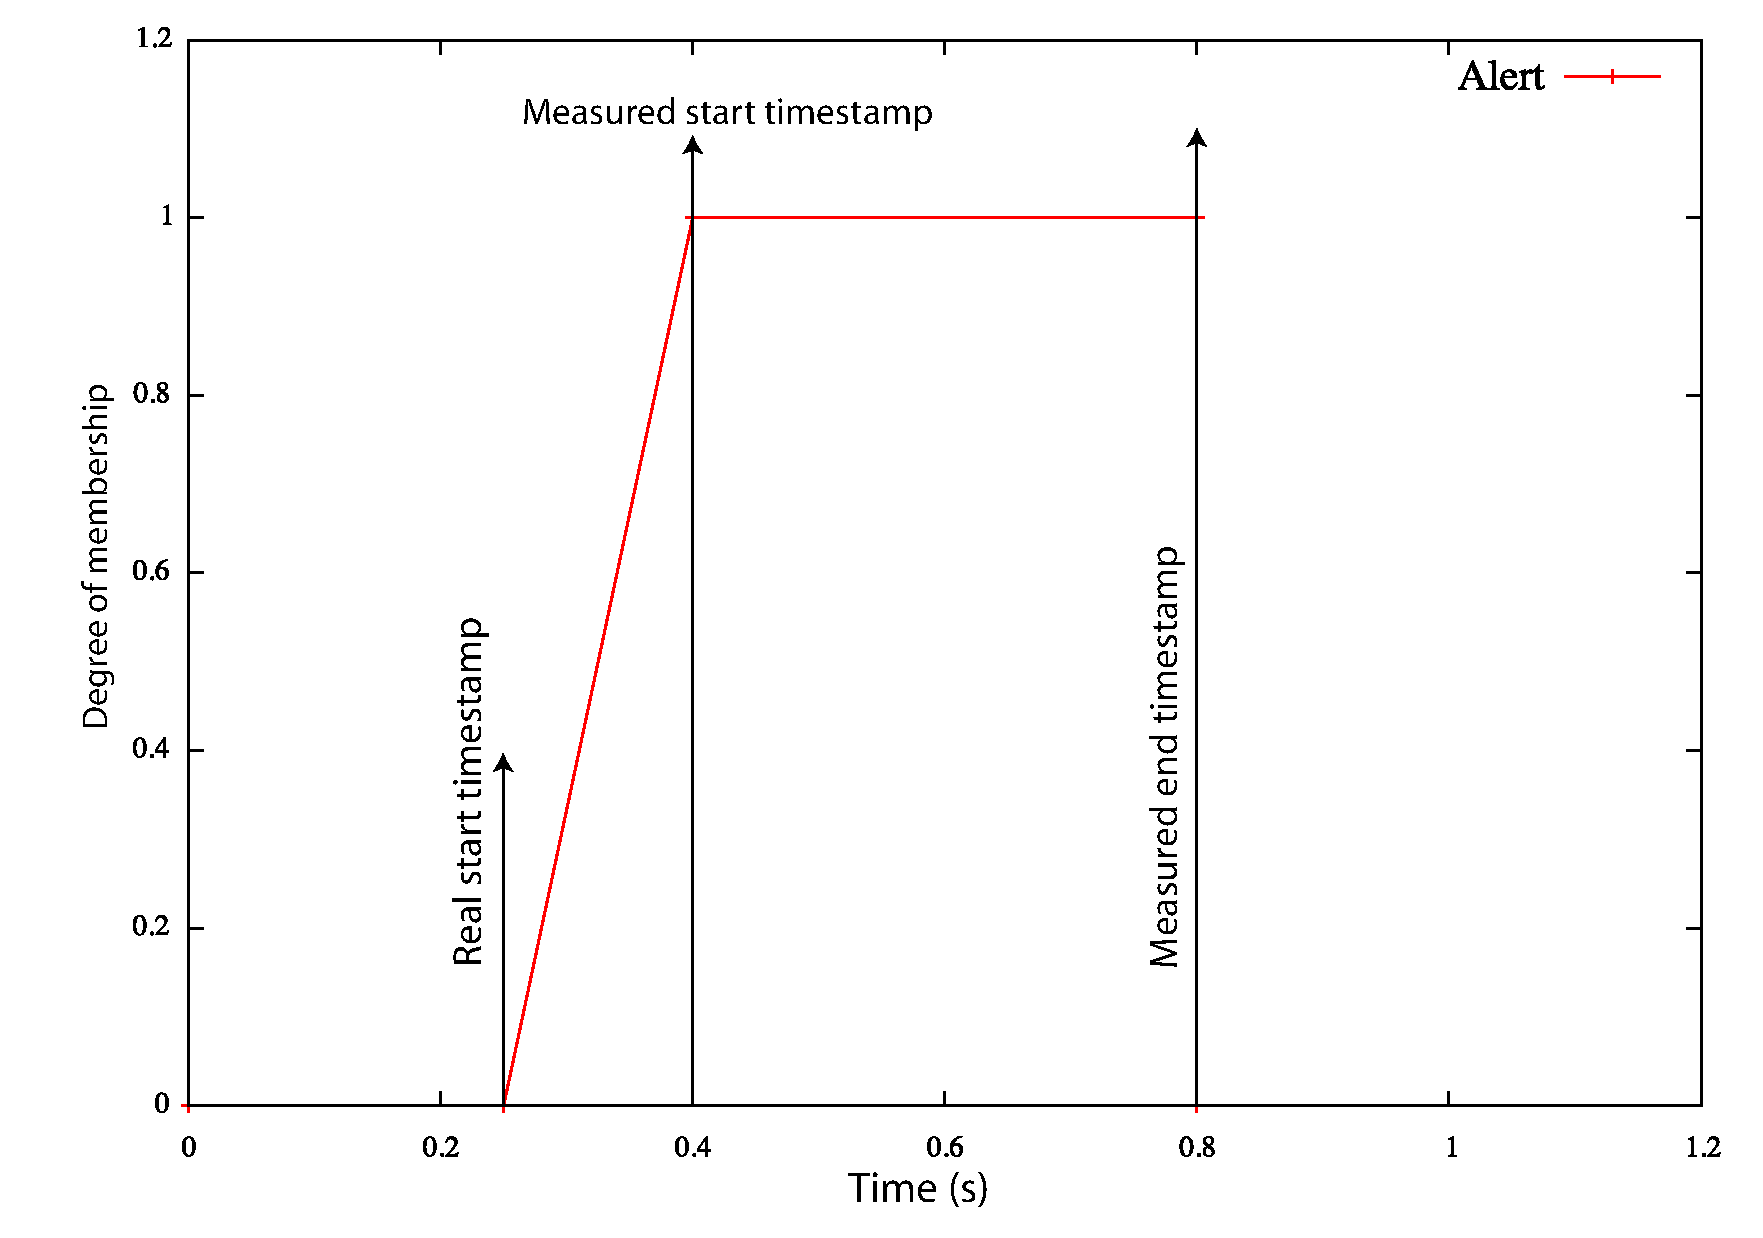
\includegraphics[width=\textwidth]{figures/correlation/fusion/fuzzy_alert_trapez}
  \caption{Non-zero long alert: uncertainty on measured timestamps are modeled.}
  \label{fig:fuzzy_alert_trapez}
\end{figure}

\subsubsection{Alert pruning}
\label{correlation:fusion:fuzzy-based-pruning}
As suggested by the \ac{IDMEF}\index{IDMEF} \texttt{Confidence} attribute both the \ac{IDS} described in Chapter~\ref{host} and \citep{zanero-savaresi,zanero-pattern} --- that we also use in the following experiments --- feature an \texttt{attack\_belief} value. For a generic alert $a$ the \texttt{attack\_belief} represents the deviation of the anomaly score, $a.score$, from the threshold, $T$. The concept of anomaly score is typical of anomaly detectors and, even if there is no agreement about its definition, it can intuitively interpreted as an internal, absolute indicator of abnormality. To complete our approach we consider the \texttt{attack\_belief} attribute for alert pruning, after the aggregation phase.

Many \acp{IDS}\index{IDS}, including the ones that we proposed, rely on probabilistic scores and thresholds in order to isolate anomalies from normal activity; thus, we implemented a first naive belief measure:

\begin{equation}\label{eq:bel}
  \mathrm{Bel}(a) = |a.score - T_{anomaly}| \in [0, 1]
\end{equation}

We remark that $a.score \in [0,1] \wedge T_{anomaly} \in [0,1] \Rightarrow \mathrm{Bel}(a) \in [0, 1]$. Also note that in the belief theory \citep{fuzzymeasure,folger_klir} $\mathrm{Bel}(B)$ indicates the belief associated to the hypothesis (or proposition) $B$; with an abbreviate notation, we indicate $\mathrm{Bel}(a)$ meaning the belief of the proposition ``the alert $a$ is associated to a real anomaly''. In this case, the domain of discourse is the set of all the alerts, which contains both the alerts that are real anomalies and the alerts that are not.

The belief theory has been used to implement complex decision support systems, such as \citep{mycin}, in which a more comprehensive belief model has been formalized taking into account both belief and misbelief. The event (mis)belief basically represents the amount of evidence is available to support the (non-)occurrence of that event. In a similar vein, we exploit both the belief and the \emph{a-priori} misbelief, the \ac{FPR}. The \ac{FPR} tells how much the anomaly detector is likely to report false alerts (i.e., the \emph{a-priori} probability of reporting false alerts, or the so called \emph{type I error}), thus it is a good candidate for modeling the misbelief of the alert. The more the \ac{FPR} increases, the more the belief associated to an alert should decrease. In the first place, such intuition can be formalized using a linear-scaling function:

\begin{equation}\label{eq:bel_lin}
  \mathrm{Bel}_{lin}(a) = (1-\underbrace{FPR}_{\mathrm{misbelief}})\mathrm{Bel}(a)
\end{equation}

However, such a scaling function (see, dashed-line plot in Figure \ref{fig:bel_fpr}) makes the belief to decrease too fast w.r.t. the misbelief. As Figure \ref{fig:bel_fpr} shows, a smoother rescaling function is the following:

\begin{equation}\label{eq:bel_exp}
  \mathrm{Bel}_{exp}(a) = (1-FPR) \mathrm{Bel}(a) e^{FPR}
\end{equation}

\begin{figure}[t]
  \centering
  
  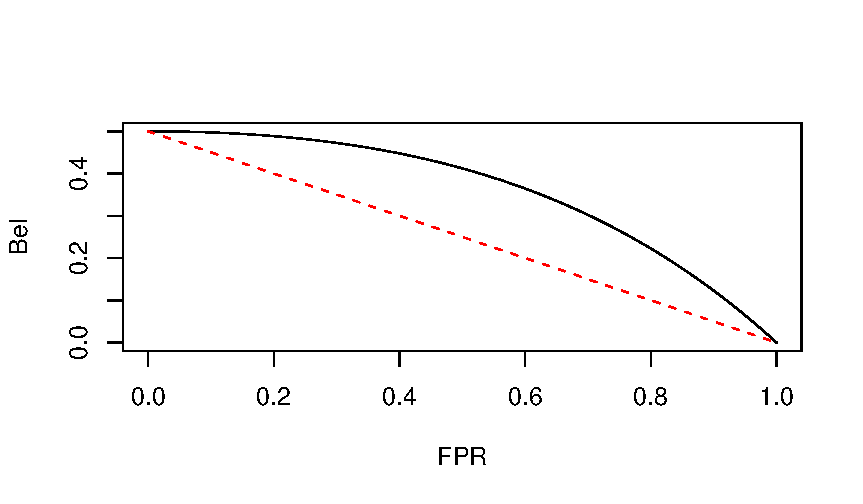
\includegraphics[width=0.8\textwidth]{figures/correlation/fusion/bel_fpr}
  
  \caption{A sample plot of $\mathrm{Bel}_{exp}(a)$ (with $|a.score -
    T_{anomaly}|, FPR \in [0,1]$) compared to a linear scaling
    function, i.e. $\mathrm{Bel}_{lin}(a)$ (dashed line)}
  \label{fig:bel_fpr}
\end{figure}

The above defined \texttt{attack\_belief} is exploited to further
reduce the resulting set of alerts. Alerts are reported only if

\begin{displaymath}
  a_{i}.attack\_belief > T_{bel}
\end{displaymath}

\noindent where $T_{bel}$ must be set to reasonable values according
to the particular environment (in our experiments we used 0.66). The
attack belief variable may be modeled using fuzzy variables with, for
example, three membership functions labeled as ``Low'', ``Medium'',
and ``High'' (\ac{IDMEF}\index{IDMEF} uses the same three-values
assignment for each alert \texttt{Confidence} attribute and we used
crisp numbers for it), but this has not been implemented yet in our
working prototype.

Let us now to summarize the incremental approaches; the first
``\emph{naive time-distance}'' uses a crisp window (as in Figure
\ref{fig:crisp_fuzzy_distance} (a)) to groups alerts w.r.t. their
timestamps. The second approach, called ``\emph{fuzzy
  time-distance}'', extends the first method: it relies on fuzzy sets
(as shown in Figure \ref{fig:crisp_fuzzy_distance} (b)) to take into
account uncertainty on timestamping and window sizing. The last
version, ``\emph{fuzzy time-distance with belief-based alert
  pruning}'', includes the last explained criterion. In the following
we will show the results of the proposed approaches on a realistic
test bench we have developed using alerts generated by our
\ac{IDS}\index{IDS} on the complete \ac{IDEVAL}\index{IDEVAL} testing
dataset (both host and network data).

\section{Mitigating Evaluation Issues}
\label{correlation:evaluation}
This section investigates the problem of testing an alert fusion engine. In order to better understand the data we used, the experimental setup is here detailed and, before reporting the results obtained with the fuzzy approach introduced, we also briefly sketch the theoretical foundations, the accuracy, and the peculiarities of the overall implementation of the \acp{IDS}\index{IDS} used for gathering the alerts. At the end of the section, we compare the results of the aggregation phase in comparison with an analysis of the accuracy of an alternative fusion approach \citep{dblp:conf/raid/qinl03}.

\subsection{A common alert representation}
\label{correlation:evaluation:representation}
The output format of our prototypes has been designed with \ac{IDMEF}\index{IDMEF} in mind, to make the normalization process --- the first step Figure~\ref{fig:correlation_model} --- as straightforward as possible. Being more precise, alerts are reported by our tools as a modified version of the original \textsf{Snort} \citep{snortsite} alert format, in order to take into account both the peculiarities of the anomaly detection approach, namely the lack of attacks name, and suggestions from the \ac{IDMEF}\index{IDMEF} data model. In this way, our testing tools can easily implement conversion procedures from and to \ac{IDMEF}\index{IDMEF}.

Basically, we represent an alert as a tuple with the following 9 attributes:

\begin{center}\footnotesize\ttfamily
  (ids\_id, src, dst, ids\_type, start\_ts, end\_ts, attack\_class, attack\_bel, target\_resource)
\end{center}

The \texttt{ids\_id} identifies the \ac{IDS}\index{IDS}, of type \texttt{ids\_type} (host or network), that has reported the alert; \texttt{src} and \texttt{dst} are the \ac{IP}\index{IP} source and destination addresses, respectively; \texttt{start\_ts} and \texttt{end\_ts} are the detection \ac{NTP}\index{NTP} \citep{RFC1305} timestamps: they are both mandatory, even if the alert duration is unknown (i.e., \texttt{start\_ts} equals \texttt{end\_ts}). The discrete attribute \texttt{attack\_class} (or name) indicates the name of the attack (if known); anomaly detectors cannot provide such an information because recognized attacks names are not known, by definition. Instead, anomaly detectors are able to quantify ``how anomalous an activity is'' so we exploited this characteristic and defined the \texttt{attack\_belief}. Finally, the \texttt{target\_resource} attribute stores the \ac{TCP}\index{TCP} port (or service name), if known, or the program begin attacked. An example instance is the following one:

\begin{center}\footnotesize\ttfamily
  (127.0.0.1-z7012gf, 127.0.0.1, 127.0.0.1, H, 0xbc723b45.0xef449129, 0xbc723b45.0xff449130, -, 0.141044, fdformat(2351))
\end{center}

The example reports an attack detected from an host \ac{IDS}\index{IDS} (\texttt{ids\_type = H}), identified by \texttt{127.0.0.1-z7012gf}: the attack against \texttt{fdformat} is started at NTP-second 0xbc723b45 (picosecond 0xef449129) and finished at NTP-second 0xbc723b45 (picosecond 0xff449130); the analyzer detected the activity as an attack with a belief of 14.1044\%. An equivalent example for the network \ac{IDS}\index{IDS} (\texttt{ids\_type = N}) anomaly detector would be something like:

\begin{center}\footnotesize\ttfamily
  (172.16.87.101/24-a032j11, 172.16.87.103/24, 172.16.87.100/24, N, 0xbc723b45.0xef449129, 0xbc723b45.0xff449130, -, 0.290937, smtp)
\end{center}

Here the attack is against the \texttt{smtp} resource (i.e., protocol) and the analyzer believes there is an attack at 29.0937\%.

\subsection{Proposed Evaluation Metrics}
\label{correlation:evaluation:framework}
Alert fusion is a relatively new problem, thus evaluation techniques are limited to a few approaches \citep{correlation_evaluation}. The development of solid testing methodologies is needed from both the theoretical and the practical points of view (a problem shared with \ac{IDS}\index{IDS} testing).

The main goal of fusion systems is to reduce the amount of alerts the security analyst has to check. In doing this, the \emph{global} \ac{DR} should ideally not decrease while the \emph{global} \ac{FPR} should be reduced as much as possible. This suggests that the first sub-goal of fusion systems is the \emph{reduction} of the \emph{global} \ac{FPR} (for instance, by reducing the total number of alerts fired by source \ac{IDS}\index{IDS} through a rejection mechanism). Moreover, the second sub-goal is to limit the decreasing of the \emph{global} \ac{DR}\index{DR}. Let us now formalize the concepts we just introduced.

We indicate with $\mathbb{A}_{i}$ the \emph{alert set} fired by the $i$-th \ac{IDS}\index{IDS}. An \emph{alert stream} is actually a structure $\langle\mathbb{A}_{i}, \prec\rangle$ over $\mathbb{A}_{i}$, where the binary relation $\prec$ means ``occurs before''. More formally

\begin{eqnarray*}
 &&\forall a, a' \in \mathbb{A}_{i}: a \prec a' \Rightarrow a.start\_ts < a'.start\_ts.
\end{eqnarray*}

\noindent with $a.start\_ts, a'.start\_ts \in \mathbb{R}^{+}$. We
assume that common operations between sets such as the union $\cup$
preserves the order or, otherwise, that the order can be recomputed;
hence, given the union between two alert sets $\mathbb{A}_{k} =
\mathbb{A}_{i} \cup \mathbb{A}_{j}$, the alert stream (i.e., ordered
set) can be always reconstructed.

In the second place, we define the two functions $d: \mathbb{A} \times \mathbb{O} \mapsto [0, 1]$, $f: \mathbb{A} \times \mathbb{O} \mapsto [0, 1]$ representing the computation of the \ac{DR} and the \ac{FPR}, respectively, that is: $DR_{i} = \mathrm{d}(\mathbb{A}_{i}, \hat{\mathbb{O}})$, $FPR_{i} = \mathrm{f}(\mathbb{A}_{i}, \hat{\mathbb{O}})$. The set $\mathbb{O}$ contains each and every true alert; $\hat{\mathbb{O}}$ is a particular instance of $\mathbb{O}$ containing alerts occurring in the system under consideration (i.e., those listed in the truth file). We can now define the \emph{global} DR, $DR_{\mathbb{A}}$, and the \emph{global} \ac{FPR}, $FPR_{\mathbb{A}}$, as:

\begin{eqnarray}\label{eq:global_dr_fpr}
  \mathbb{A} & = & \bigcup_{i \in I} \mathbb{A}_{i}\\
  DR_{\mathbb{A}} & = & \mathrm{d}\left(\mathbb{A}, \hat{\mathbb{O}}\right)\\
  FPR_{\mathbb{A}} & = & \mathrm{f}\left(\mathbb{A}, \hat{\mathbb{O}}\right)
\end{eqnarray}

The output of a generic alert fusion system, is another alert stream $\mathbb{A}'$ with $|\mathbb{A}'| \leq |\mathbb{A}|$; of course, $|\mathbb{A}'| = |\mathbb{A}|$ is a degenerative case. To measure the ``impact'' of an alert fusion system we define the \ac{ARR} which quantifies:

\begin{eqnarray}\label{eq:arr}
  ARR = \frac{|\mathbb{A}'|}{|\mathbb{A}|}.
\end{eqnarray}

The aforementioned sub-goals can now be formalized into two performance metrics. The ideal correlation system would maximize both $ARR$ and $\frac{DR_{\mathbb{A'}}}{DR_{\mathbb{A}}}$; meanwhile, it would minimize $\frac{FPR_{\mathbb{A'}}}{FPR_{\mathbb{A}}}$. Of course, $ARR = 1$ and $ARR = 0$ are degenerative cases. Low (i.e., close to $0.0$) $\frac{FPR_{\mathbb{A'}}}{FPR_{\mathbb{A}}}$ means that the fusion system has significantly decreased the original \ac{FPR}; in a similar vein, high (i.e., close to $1.0$) $\frac{DR_{\mathbb{A'}}}{DR_{\mathbb{A}}}$ means that, while reducing false positive alerts, the loss of detection capabilities is minimal.

\begin{figure}[p]
  \centering
  
  \subfloat[][]{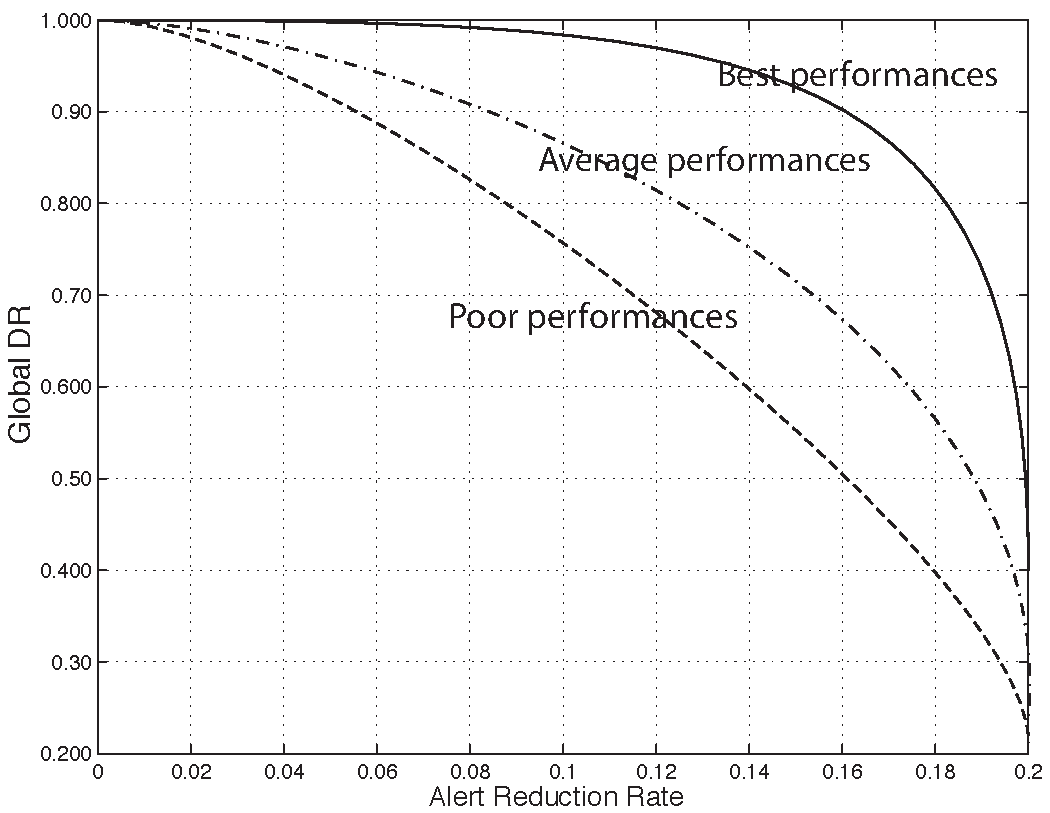
\includegraphics[width=0.8\textwidth]{figures/correlation/evaluation/dummy_dr}\label{subfig:dummy-dr}}
  
  \subfloat[][]{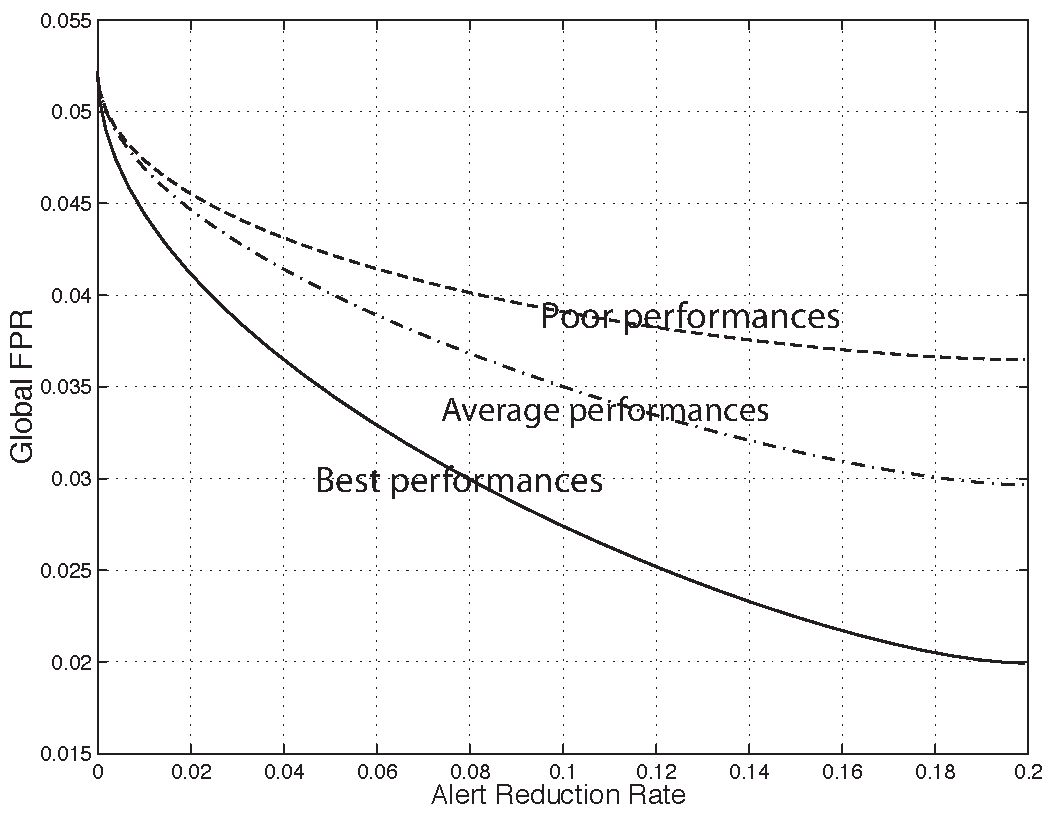
\includegraphics[width=0.8\textwidth]{figures/correlation/evaluation/dummy_fpr}\label{subfig:dummy-fpr}}

  \caption{Hypothetical plots of \subref{subfig:dummy-dr} the global
    DR, $DR_{\mathbb{A}'}$, vs. $ARR$ and \subref{subfig:dummy-fpr}
    the global FPR, $FPR_{\mathbb{A}'}$, vs. $ARR$.}
  \label{fig:dummy}
\end{figure}

Therefore, a fusion system is better than another if it has
\emph{both} a greater $\frac{DR_{\mathbb{A}'}}{DR_{\mathbb{A}}}$ and a
lower $\frac{FPR_{\mathbb{A}'}}{FPR_{\mathbb{A}}}$ rate than the
latter. This criterion by no means has to be considered as complete or
exhaustive. In addition, it is useful to compare $DR_{\mathbb{A}'}$
and $FPR_{\mathbb{A}'}$ plots, vs. $ARR$, of different correlation
systems obtaining diagrams like the one exemplified in Figure
\ref{fig:dummy}; this gives a graphical idea of which correlation
algorithm is better. For instance, Figure \ref{fig:dummy} show that
the algorithm labeled as \textsf{Best performances} is better than the
others, because it shows higher $FPR_{\mathbb{A}'}$ reduction while
$DR_{\mathbb{A}'}$ does not significantly decrease.

\begin{note}[Configuration parameters]
  One limitation of our approach is that it relies on the attack
  belief threshold. Currently, there is no rigorous procedure for
  deriving it in practice. In our experiments, we run the aggregation
  algorithm several times on the same data-set under the same
  conditions until acceptable values of DR and FPR.

  Similarly, the current version of our algorithm relies on alpha cut
  values for deciding whether or not two alerts can be fused or
  not. However, note that this is different from setting thresholds on
  time, e.g., fusing alerts that are delayed, say, 60 seconds. In
  fact, such a threshold would have \emph{direct} impact on the fusion
  procedure; instead, different values of alpha cuts and shapes of
  trapezoid fuzzy sets have a much smoother effects on the results. In
  addition, a user of our system may not be aware of what does it
  means for two alerts to be, say, 60-seconds-close in time; it might
  be easier for the user to just configure the system to fuse alerts
  that are 50\%-close.
\end{note}

\subsection{Experimental Results}
\label{sec:anom-detect-prot}
In these experiments we used two prototypes for network- and
host-based anomaly detection. In particular, we use the system
described in Chapter~\ref{host} (host-based) and
\citep{zanero-savaresi,zanero-pattern} (network-based). These tools
were used to generate alert streams for testing the three variants of
the fuzzy aggregation algorithm we proposed. The same tools were also
used to generate alerts data for testing our correlation algorithm
detailed in Section~\ref{correlation:causality}.

Because of the well known issues of \ac{IDEVAL}\index{IDEVAL} and to
avoid biased interpretation of the results, in our testing we used the
\ac{IDEVAL}\index{IDEVAL} dataset with the following simplification:
we just tried to fuse the stream of alerts coming from a
\ac{HIDS}\index{HIDS} sensor and a \ac{NIDS}\index{NIDS} sensor, which
is monitoring the whole network. To this end, we ran the two
prototypes on the whole 1999 \ac{IDEVAL}\index{IDEVAL} testing
dataset, using the network dumps and the host-based logs from
\texttt{pascal}. We ran the \ac{NIDS}\index{NIDS} prototype on
\texttt{tcpdump} data and collected 128 alerts for attacks against the
host \texttt{pascal.\-eyrie.\-af.\-mil}. The \ac{NIDS}\index{NIDS}
also generated 1009 alerts related to other hosts. Using the
\ac{HIDS}\index{HIDS} prototype we generated 1070 alerts from the
dumps of the host \texttt{pascal.\-eyrie.\-af.\-mil}. The
\ac{NIDS}\index{NIDS} was capable of detecting almost 66\% of the
attacks with less than 0.03\% of false positives; the
\ac{HIDS}\index{HIDS} performs even better with a \ac{DR} of 98\% and
1.7\% of false positives. However, in this experiment we focus on the
aggregated results rather than the detection capabilities of the
single system.

In the following, we use this shorthand notation: $Net$ is the
substream of all the alerts generated by the
\ac{NIDS}\index{NIDS}. $HostP$ is the substream of all the alerts
generated by the \ac{HIDS}\index{HIDS} installed on
\texttt{pascal.\-eyrie.\-af.\-mil}, while $NetP$ regards all the
alerts (with \texttt{pascal} as a target) generated by the
\ac{NIDS}\index{NIDS}; finally, $NetO = Net \backslash NetP$ indicates
all the alerts (with all but \texttt{pascal} as a target) generated by
the \ac{NIDS}\index{NIDS}.

Using the data generated as described above, and the metrics proposed
in Section~\ref{correlation:evaluation:framework}, we compared three
different versions of the alert aggregation algorithms described in
Section \ref{correlation:fusion}. In particular we compare the use of
crisp time-distance aggregation, the use use of a simple fuzzy
time-distance aggregation; and finally, the use of
\texttt{attack\_belief} for alert pruning.

Numerical results are plotted in in Figure \ref{fig:dr_fpr} for
different values of $ARR$. As we discussed in
Section~\ref{correlation:evaluation}, Figure \ref{fig:dr_fpr} (a)
refers to the reduction of \ac{DR} while Figure \ref{fig:dr_fpr} (b)
focuses on \ac{FPR}. $DR_{\mathbb{A}'}$ and $FPR_{\mathbb{A}'}$ were
calculated using the complete alert stream, network and host, at
different values of $ARR$. The values of $ARR$ are obtained by
changing the parameters values: in particular, we set $T_{bel}=0.66$,
the alpha cut of $T_{near}$ to $0.5$, the window size to $1.0$
seconds, and varied the smoothing of the trapezoid between $1.0$ and
$1.5$ seconds, and the alert delay between $0$ and $1.5$ seconds. It
is not useful to plot the increase in false negatives, as it can be
easily deduced from the decrease in \ac{DR}\index{DR}.

\begin{figure}[p]
  \centering
  
  \subfloat[][]{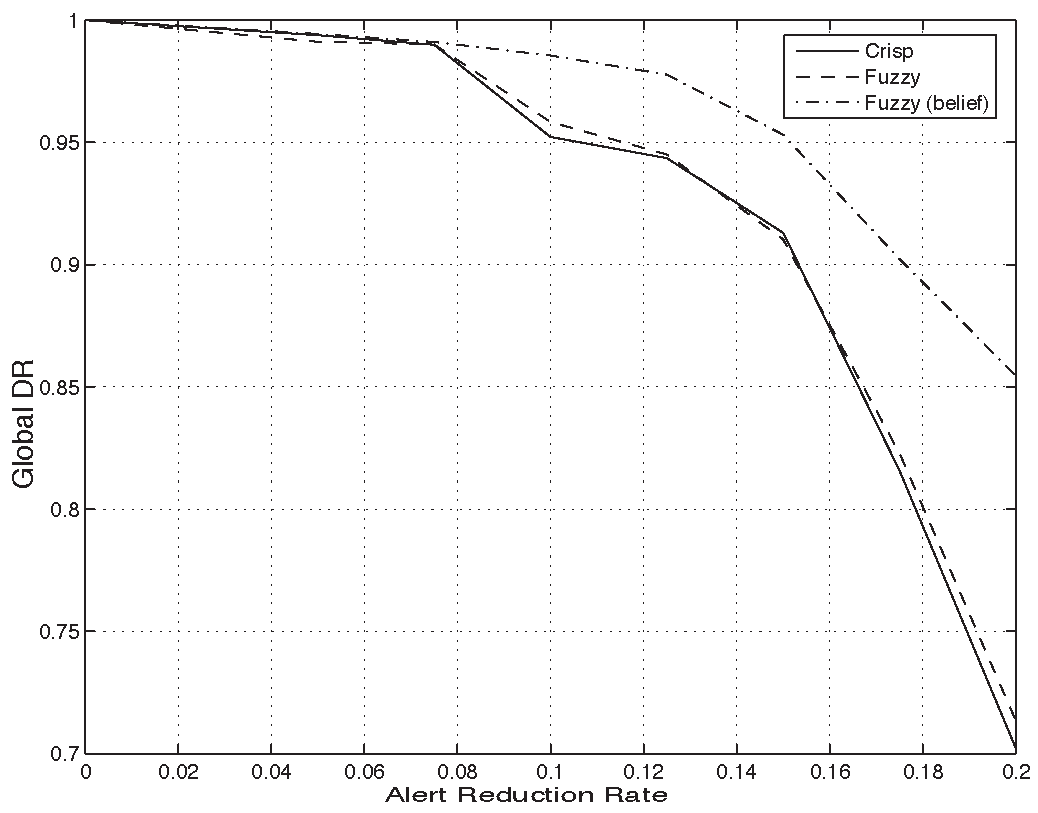
\includegraphics[width=0.8\textwidth]{figures/correlation/fusion/dr_ccf}}
  
  \subfloat[][]{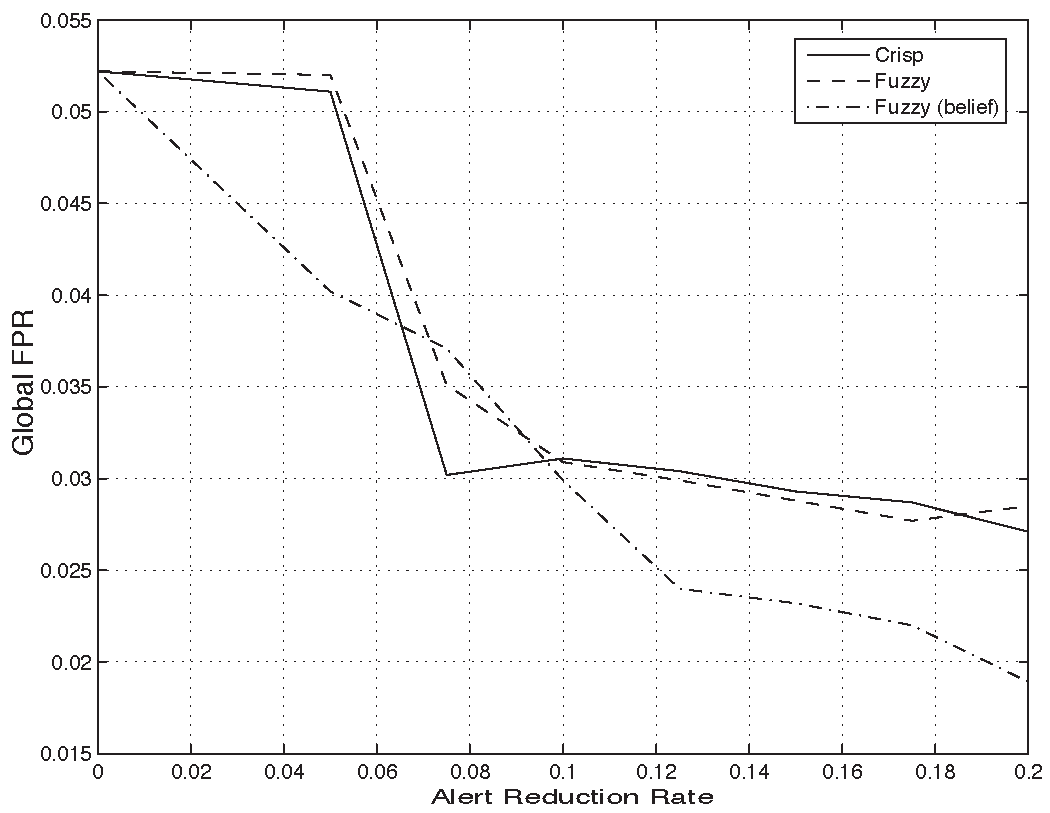
\includegraphics[width=0.8\textwidth]{figures/correlation/fusion/fpr_ccf}}
  
  \caption{Plot of the $DR_{\mathbb{A}'}$ (a) and $FPR_{\mathbb{A}'}$
    (b) vs. $ARR$. ``Crisp'' refers to the use of the crisp
    time-distance aggregation; ``Fuzzy'' and ``Fuzzy (belief)''
    indicates the simple fuzzy time-distance aggregation and the use
    of the \texttt{attack\_belief} for alert discarding,
    respectively.}
  \label{fig:dr_fpr}
\end{figure}

The last aggregation algorithm, denoted as ``Fuzzy (belief)'', shows better performances since the $DR_{\mathbb{A}'}$ is always higher w.r.t. the other two aggregation strategies; this algorithm also causes a significant reduction of the $FPR_{\mathbb{A}'}$. Note that, taking into account the \texttt{attack\_belief} attribute makes the difference because it avoids true positives to be discarded; on the other hand, \emph{real} false positive are not reported in the output alert stream because of their low belief.

It is difficult to properly compare our approach with other other fusion approaches proposed in the reviewed literature, because the latter were not specifically tested from the aggregation point of view, separately from the correlation one. Since the prototypes used to produce results are not released, we are only able to compare our approach with the \emph{overall} fusion systems presented by others. 

\section{Using Non-parametric Statistical Tests}
\label{correlation:causality}
In this section we analyze the use of different types of statistical
tests for the correlation of anomaly detection alerts. We show that
the technique proposed in \citep{dblp:conf/raid/qinl03} and summarized
in Section~\ref{detection:correlation}, one of the few proposals that
can be extended to the anomaly detection domain, strongly depends on
good choices of a parameter which proves to be both sensitive and
difficult to estimate. Rather than using the \acf{GCT} we propose
alternative approach \citep{MaggiZaneroRAID07} based on a set of
simpler statistical tests. We proved that our criteria work well on a
simplified correlation task, without requiring complex configuration
parameters. More precisely, in \citep{MaggiZaneroRAID07} we explored
the use of \emph{statistical causality tests}, which have been
proposed for the correlation of \ac{IDS}\index{IDS} alerts, and which
could be applied to anomaly based \ac{IDS}\index{IDS} as well. We
redefine the problem in terms of a simpler statistical test, and
experimentally validate it.

\subsection{The Granger Causality Test}
\label{correlation:causality:grang-caus-test}
We tested the sensitivity of the \ac{GCT}\index{GCT} to the choice of
two parameters: the sampling time of the time series that represent
the alerts, $w$, and the time lag $l$, i.e., the order of the
\ac{AR}\index{AR} model being fitted. In \citep{dblp:conf/raid/qinl03}
the sampling time was arbitrarily set to $w = 60s$, while the choice
of $l$ is not documented. However, our experiments show that the
choice of these parameters can strongly influence the results of the
test. As explained in \citep{2009_maggi_zanero_matteucci_fusion},
other values of $l$ lead to awkward results.

We used the same dataset described in Section~\ref{sec:anom-detect-prot}, with the following approach: we tested if $NetP$ has any causal relationship\footnote{In the following we will use the symbol ``$\leadsto$'' to denote ``Granger-causes'' so, for instance, ``A $\leadsto$ B'' has to be read as ``A causes B''; the symbol ``$\cancel{\leadsto}$'' indicates the negated causal relationship, i.e., ``does not Granger-cause''.} with $HostP$; we also tested $HostP$ $\cancel{\leadsto}$ $NetP$. Since only a reduced number of alerts was available and since it was impossible to aggregate alerts along the ``attack name'' attribute (unavailable on anomaly detectors), we preferred to construct only two, large time series: one from $NetP$ (denoted as $NetP(k)$) and one from $HostP$ (denoted as $HostP(k)$). In the experiment reported in \citep{dblp:conf/raid/qinl03} the sampling time, $w$, has been fixed at 60 seconds, although we tested different values from 60 to 3600 seconds. In our simple experiment, the expected result is that $NetP \leadsto HostP$, and that $HostP \not\leadsto NetP$ (the $\leadsto$ indicates ``causality'' while $\not\leadsto$ is its negation).

Since the first experiment ($w = 60$) led us to unexpected results (i.e., using a lag, $l$, of $3$ minutes, both $NetP(k)$ $\cancel{\leadsto}$ $HostP(k)$, and vice versa) we decided to plot the test results (i.e., p-value and \ac{GCI}) vs. both $l$ and $w$. In Figure \ref{fig:minute_a0} (a) $l$ is reported in minutes while the experiment has been performed with $w = 60s$; the dashed line is the $p$-value of the test ``$NetP(k)$ $\leadsto$ $HostP(k)$'', the solid line is opposite one. As one may notice, neither the first nor the second test passed, thus nothing can be concluded: fixing the test significance at $\alpha = 0.20$ is the only way for refusing the null hypothesis (around $l \simeq 2.5$ minutes) to conclude both that $NetP \leadsto HostP$'' and that $HostP \cancel{\leadsto} NetP$; the \ac{GCI}\index{GCI} plotted in Figure \ref{fig:minute_a0} (b) confirms the previous result. However, for other values of $l$ the situation changes leading to opposite results.

Figure \ref{fig:hh_a0} shows the results of the test for $w = 1800$ seconds and $l \in [50, 300]$ minutes. If we suppose a test significance of $\alpha = 0.05$ (dotted line), for $l \simeq 120$ the result is that $HostP \leadsto NetP$ while $NetP \cancel{\leadsto} HostP$, the opposite of the previous one. Moreover, for other values of $l$ the $p$-value leads to different results.

The last experiment results are shown in Figure \ref{fig:h_a0}: for $l
> 230$ minutes, one may conclude that $NetP$ $\leadsto$ $HostP$ and
$HostP$ $\cancel{\leadsto}$ $NetP$; i.e., the expected result, even if
the p-value for the second test is close to $\alpha = 0.05$.

\begin{figure}[p]
  \centering
  
  \subfloat[][]{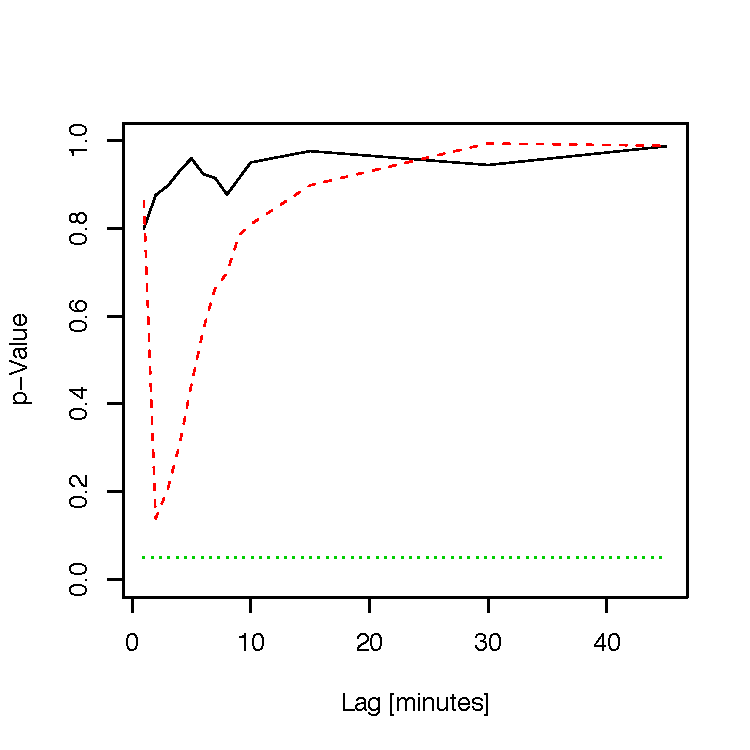
\includegraphics[width=0.8\textwidth]{figures/correlation/fusion/granger/pvalue_minute_a0}}
  
  \subfloat[][]{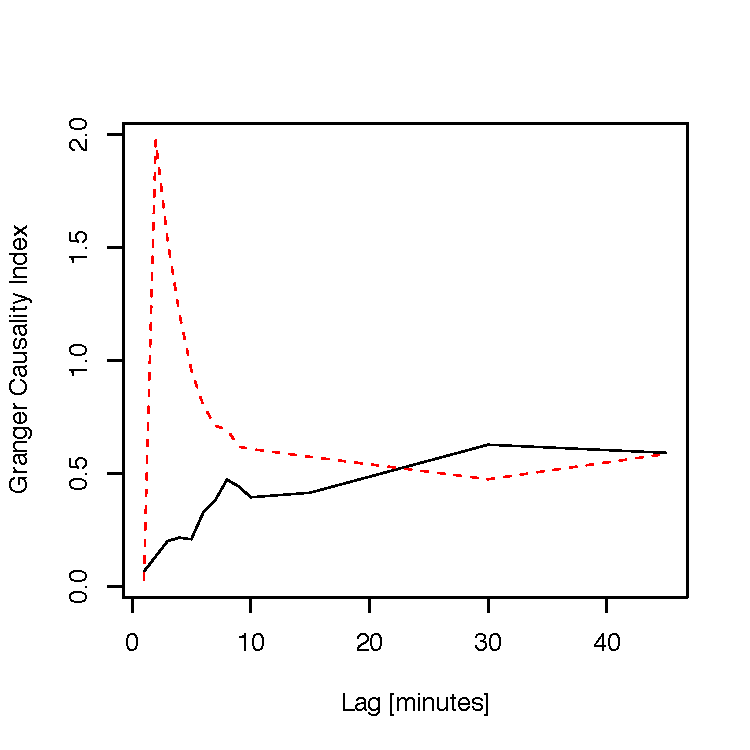
\includegraphics[width=0.8\textwidth]{figures/correlation/fusion/granger/gci_minute_a0}}
  
  \caption{p-value (a) and \ac{GCI} (b) vs. $l$ (in minutes) for the
    first \ac{GCT} experiment ($w = 60.0$ seconds): ``$NetP(k)
    \leadsto HostP(k)$'' (dashed line), ``$HostP(k) \leadsto
    NetP(k)$'' (solid line).}
  \label{fig:minute_a0}
\end{figure}

The previous experiments show only that the \ac{GCT} failed on the dataset we generated, not that it does not work well in general. It may be the case that it is not suitable for ``blind'' alerts (i.e., without any information about the attack) reported by anomaly detectors: in fact, \citep{dblp:conf/raid/qinl03} used time series built from hyper-alerts resulting from an aggregation along \emph{all} attributes: instead, in the anomaly-based case, the lack of attack names does not allow such hyper-alerts to be correctly constructed. In any case, the test result significantly depends on $l$ (i.e., the test is asymptotic); this means that an appropriate choice of $l$ will be required, depending on specific environmental conditions. The optimal $l$ is also likely to change over time in a given environment.

\begin{figure}[p]
  \centering
  
  \subfloat[][]{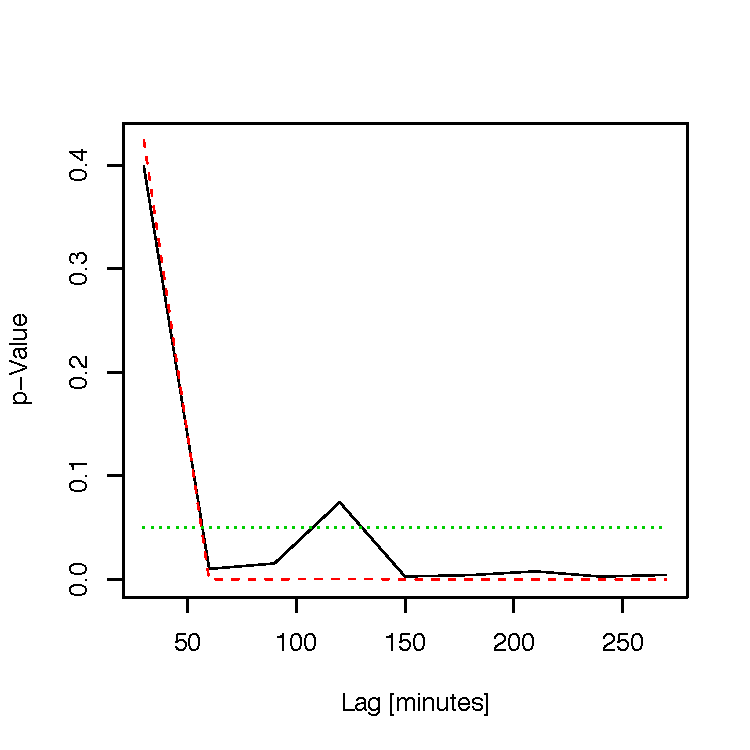
\includegraphics[width=0.8\textwidth]{figures/correlation/fusion/granger/pvalue_hh_a0}}
  
  \subfloat[][]{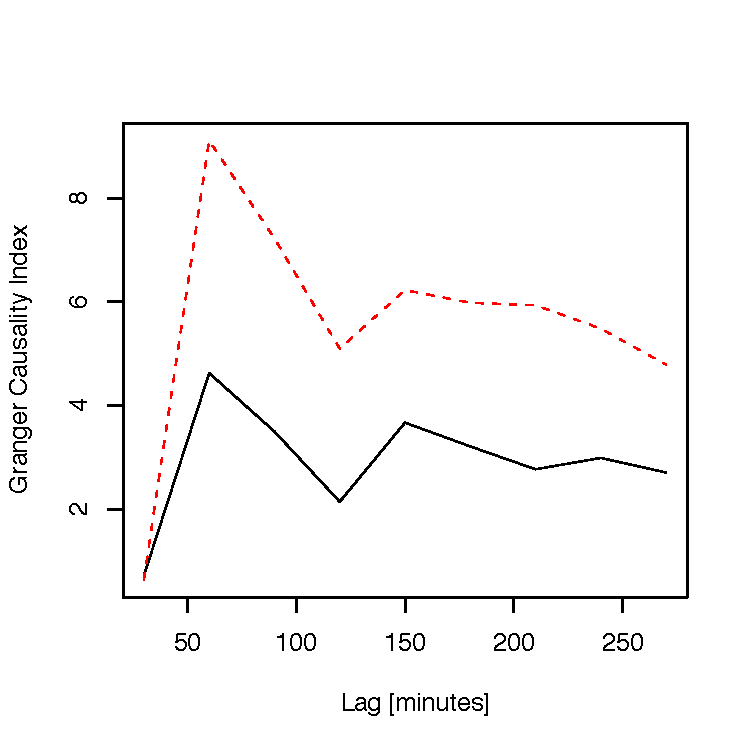
\includegraphics[width=0.8\textwidth]{figures/correlation/fusion/granger/gci_hh_a0}}
  
  \caption{p-value (a) and \ac{GCI}\index{GCI} (b) vs. $l$ (in
    minutes) for the first Granger causality test experiment ($w =
    1800.0$ seconds): ``$NetP(k) \leadsto HostP(k)$'' (dashed line),
    ``$HostP(k) \leadsto NetP(k)$'' (solid line).}
  \label{fig:hh_a0}
\end{figure}

A possible explanation is that the \ac{GCT}\index{GCT} is significant only if both the linear regression models are optimal, in order to calculate the correct residuals. If we use the \ac{AIC} \citep{akaike1974nls} to estimate the optimal time lag $\hat{l}$ over different windows of data, we find out that $\hat{p}$ wildly varies over time, as it is shown in Figure \ref{fig:p-does-vary}. The fact that there is no stable optimal choice of $l$, combined with the fact that the test result significantly depends on it, makes us doubt that the Granger causality test is a viable option for general alert correlation. The choice of $w$ seems equally important and even more difficult to perform, except by guessing.

\begin{figure}[p]
  \centering
  
  \subfloat[][]{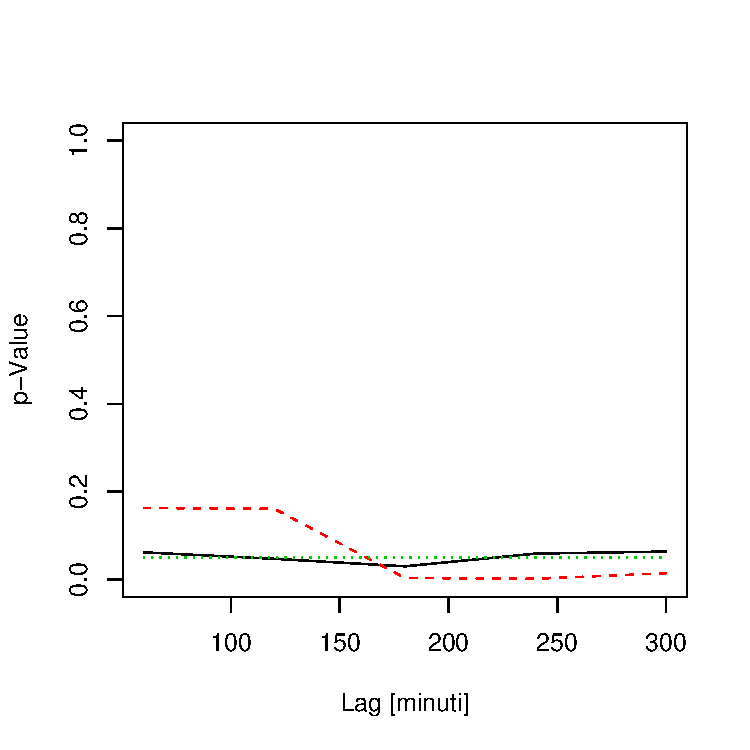
\includegraphics[width=0.8\textwidth]{figures/correlation/fusion/granger/pvalue_h_a0}}
  
  \subfloat[][]{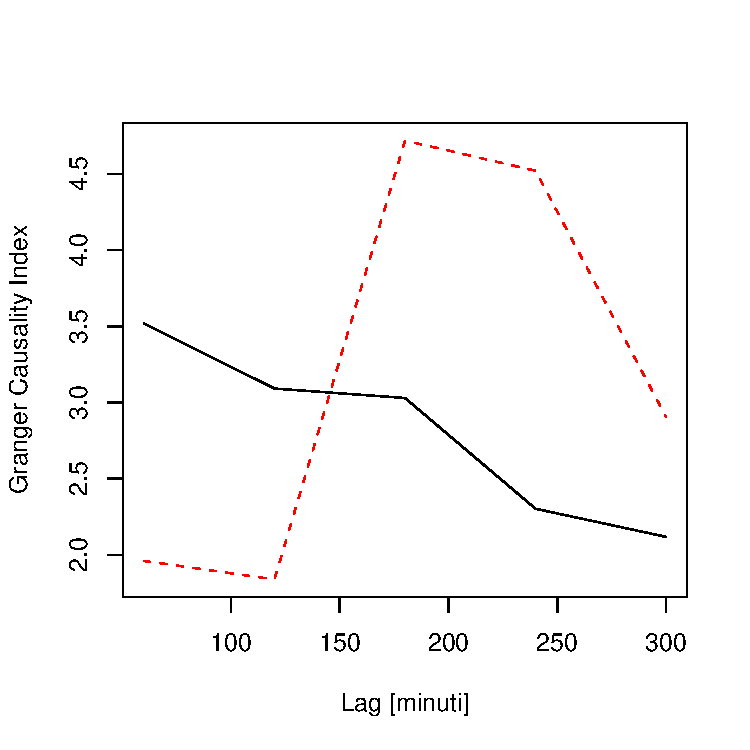
\includegraphics[width=0.8\textwidth]{figures/correlation/fusion/granger/gci_h_a0}}
  
  \caption{p-value (a) and \ac{GCI}\index{GCI} (b) vs. $l$ (in
    minutes) for the first Granger causality test experiment ($w =
    3600.0$ seconds): ``$NetP(k) \leadsto HostP(k)$'' (dashed line),
    ``$HostP(k) \leadsto NetP(k)$'' (solid line).}
  \label{fig:h_a0}
\end{figure}

Of course, our testing is not conclusive: the \ac{IDEVAL}\index{IDEVAL} alert sets may simply not be adequate for showing causal relationships. Another, albeit more unlikely, explanation, is that the \ac{GCT} test may not be suitable for anomaly detection alerts: in fact, in \citep{dblp:conf/raid/qinl03} it has been tested on misuse alerts. But in fact there are also theoretical reasons to doubt that the application of the Granger test can lead to stable, good results. First, the test is asymptotic w.r.t. $l$ meaning that the results reliability decreases as $l$ increases because of the loss of degrees of freedom. Second, it is based on the strong assumption of \emph{linearity} in the auto-regressive model fitting step, which strongly depends on the observed phenomenon. In the same way, the stationarity assumption of the model does not always hold.

\subsection{Modeling alerts as stochastic processes}
\label{correlation:causality:count-proc-model}
Instead of interpreting alert streams as time series (as proposed by
the \ac{GCT}\index{GCT}-based approach), we propose to change point of
view by using a stochastic model in which alerts are modeled as
(random) events in time. This proposal can be seen as a formalized
extension of the approach introduced in \citep{valeur04comprehensive}
(see Figure~\ref{fig:correlation_model}), which correlates alerts if
they are fired by different \ac{IDS}\index{IDS} within a
``negligible'' time frame, where ``negligible'' is defined with a
crisp, fixed threshold.

For simplicity, once again we describe our technique in the simple case of a single \ac{HIDS}\index{HIDS} and a single \ac{NIDS}\index{NIDS} which monitors the whole network. The concepts, however, can be easily generalized to take into account more than two alert streams, by evaluating them couple by couple. For each alert, we have three essential information: a timestamp, a ``target'' host (fixed, in the case of the \ac{HIDS}\index{HIDS}, to the host itself), and the generating sensor (in our case, a binary value).

With a self-explaining notation, define the following random variables: $T_{NetP}$ are the arrival times of network alerts in $NetP$ ($T_{NetO}$, $T_{HostP}$ are similarly defined); $\varepsilon_{NetP}$ ($\varepsilon_{NetO}$) are the delays (caused by transmission, processing and different granularity in detection) between a specific network-based alert regarding \texttt{pascal} (not \texttt{pascal}) and the corresponding host-based one. The actual values of each $T_{(\cdot)}$ is nothing but the set of timestamps extracted from the corresponding alert stream. We reasonably assume that $\varepsilon_{NetP}$ and $T_{NetP}$ are stochastically independent (the same is assumed for $\varepsilon_{NetO}$ and $T_{NetO}$). Figure~\ref{fig:epsilon} shows how delays between network and host alerts are calculated.

\begin{figure}[t]
  \centering
  \includegraphics[width=\textwidth]{figures/correlation/causality/p-does-vary}
  \caption{The optimal time lag $p = \hat{l}$ given by the \ac{AIC}
    criterion strongly varies over time.}
  \label{fig:p-does-vary}
\end{figure}

In an \emph{ideal} correlation framework with two equally perfect \ac{IDS}\index{IDS} with a 100\% \ac{DR} and 0\% \ac{FPR}, if two alert streams are correlated (i.e., they represent independent detections of the same attack occurrences by different \acp{IDS}\index{IDS} \citep{valeur04comprehensive}), they also are ``close'' in time. $NetP$ and $HostP$ should evidently be an example of such a couple of streams. Obviously, in the real world, some alerts will be missing (because of false negatives, or simply because some of the attacks are detectable only by a specific type of detector), and the distances between related alerts will therefore have some higher variability. In order to account for this, we can ``cut off'' alerts that are too far away from a corresponding alert in the other time series, presuming them to be singletons. In our case, knowing that single attacks did not last more than $400 s$ in the original dataset, we tentatively set a cutoff threshold at this point.

Under the given working assumptions, the proposed stochastic model is used to formalize the correlation problem as a set of two statistical hypothesis tests:

\begin{equation}\label{eq:hp-test-1}
  \begin{array}{ccc}
    H_{0} && H_{1}\\
    T_{HostP} \neq T_{NetP} + \varepsilon_{NetP} &vs.& T_{HostP} = T_{NetP} + \varepsilon_{NetP}
  \end{array}
\end{equation}

\begin{equation}\label{eq:hp-test-2}
  \begin{array}{ccc}
    T_{HostP} \neq T_{NetO} + \varepsilon_{NetO} &vs.& T_{HostP} = T_{NetO} + \varepsilon_{NetO}
  \end{array}
\end{equation}

Let $\{t_{i,k}\}$ be the observed timestamps of $T_{i}, \forall i \in \{HostP$, $NetP$, $NetO\}$, the meaning of the first test is straightforward: within a random amount of time, $\varepsilon_{NetP}$, the occurring of a host alert, $t_{HostP,k}$, is preceded by a network alert, $t_{NetP,k}$. If this does not happen for a statistically significant amount of events, the test result is that alert stream $T_{NetP}$ is \emph{uncorrelated} to $T_{HostP}$; in this case, we have \emph{enough statistical evidence} for refusing $H_{1}$ and accepting the null one. Symmetrically, refusing the null hypothesis of the second test means that the $NetO$ alert stream (regarding to all hosts but \texttt{pascal}) is correlated to the alert stream regarding \texttt{pascal}.

Note that, the above two tests are strongly related to each other: in an ideal correlation framework, it cannot happen that both ``$NetP$ is correlated to $HostP$'' and ``$NetO$ is correlated to $HostP$'': this would imply that the network activity regarding to all hosts but \texttt{pascal} (which raises $NetO$) has to do with the host activity of \texttt{pascal} (which raises $HostP$) with the same order of magnitude of $NetP$, that is an intuitively contradictory conclusion. Therefore, the second test acts as a sort of ``robustness'' criterion.

\begin{figure}[t]
  \centering
  \includegraphics[width=\textwidth]{figures/correlation/causality/epsilon}
  \caption{How delays between network and host alerts are calculated.}
  \label{fig:epsilon}
\end{figure}

From our alerts, we can compute a sample of $\varepsilon_{NetP}$ by simply picking, for each value in $NetP$, the value in $HostP$ which is closest, but greater (applying a threshold as defined above). We can do the same for $\varepsilon_{NetO}$, using the alerts in $NetO$ and $HostP$.

The next step involves the \emph{choice of the distributions} of the random variables we defined above. Typical distributions used for modeling random occurrences of timed events fall into the family of exponential \acp{PDF}\index{PDF} \citep{pestman}. In particular, we decided to fit them with Gamma \acp{PDF}\index{PDF}, because our experiments show that such a distribution is a good choice for both the $\varepsilon_{NetP}$ and $\varepsilon_{NetO}$.

\begin{figure}[t]
  \centering
  \includegraphics[width=\textwidth]{figures/correlation/causality/hist_qqplot}
  \caption{Histograms vs. estimated density (red dashes) and Q-Q
    plots, for both $\hat{f_{O}}$ and $\hat{f_{P}}$.}
  \label{fig:hist_qqplot}
\end{figure}

The estimation of the \ac{PDF}\index{PDF} of $\varepsilon_{NetP}$,
$f_{P} := f_{\varepsilon_{NetP}}$, and $\varepsilon_{NetO}$, $f_{O} :=
f_{\varepsilon_{NetO}}$, is performed using the well known \ac{ML}
technique \citep{venables2002mas} as implemented in the \textsf{GNU S}
package: the results are summarized in Figure
\ref{fig:hist_qqplot}. $f_{P}$ and $f_{O}$ are approximated by

\begin{displaymath}
  \mathrm{Gamma}(3.0606, 0.0178)
\end{displaymath}

\begin{displaymath}
  \mathrm{Gamma}(1.6301, 0.0105)
\end{displaymath}


\noindent respectively (standard errors on parameters are $0.7080$, $0.0045$ for $f_{P}$ and $0.1288$, $0.009$ for $f_{O}$). From now on, the estimator of a given density $f$ will be indicated as $\hat{f}$.

\begin{figure}[t]
  \centering
  \includegraphics[width=\textwidth]{figures/correlation/causality/hist_1998}
  \caption{Histograms vs. estimated density (red dashes) for
    both $\hat{f_{O}}$ and $\hat{f_{P}}$ (\ac{IDEVAL}\index{IDEVAL} 1998)}
  \label{fig:hist_1998}
\end{figure}

Figure \ref{fig:hist_qqplot} shows histograms vs. estimated density (red, dashed line) and quantile-quantile plots (Q-Q plots), for both $\hat{f}_{O}$ and $\hat{f}_{P}$. We recall that Q-Q plots are an intuitive graphical ``tool'' for comparing data distributions by plotting the quantile of the first distribution against the quantile of the other one.

Considering that the samples sizes of $\varepsilon_{(\cdot)}$ are around 40, Q-Q plots empirically confirms our intuition: in fact, $\hat{f}_{O}$ and $\hat{f}_{P}$ are both able to explain real data well, within inevitable but negligible estimation errors. Even if $\hat{f}_{P}$ and $\hat{f}_{O}$ are both Gamma-shaped, it must be noticed that they significantly differ in their parametrization; this is a very important result since it allows to set up a proper criterion to decide whether or not $\varepsilon_{NetP}$ and $\varepsilon_{NetO}$ are generated by the same phenomenon.

Given the above estimators, a more precise and robust hypotheses test can be now designed. The Test \ref{eq:hp-test-1} and \ref{eq:hp-test-2} can be mapped into two-sided \ac{KS} tests \citep{pestman}, achieving the same result in terms of decisions:

\begin{equation}\label{eq:ks-test-1}
  \begin{array}{ccc}
    H_{0} && H_{1}\\
    \varepsilon_{NetP} \sim f_{P} &vs.& \varepsilon_{NetP} \not\sim f_{P}
  \end{array}
\end{equation}

\begin{equation}\label{eq:ks-test-3}
  \begin{array}{ccc}
    \varepsilon_{NetO} \sim f_{O} &vs.& \varepsilon_{NetO} \not\sim f_{O}
  \end{array}
\end{equation}

where the symbol $\sim$ means ``has the same distribution of''. Since we do not know the real \acp{PDF}\index{PDF}, estimators are used in their stead. We recall that the \ac{KS}\index{KS}-test is a \emph{non-parametric} test to compare a sample (or a \ac{PDF}) against a \ac{PDF} (or a sample) to check how much they differs from each other (or how much they fit). Such tests can be performed, for instance, with \texttt{ks.test()} (a \texttt{GNU R} native procedure): resulting p-values on \ac{IDEVAL}\index{IDEVAL} 1999 are $0.83$ and $0.03$, respectively.

Noticeably, there is a significant statistical evidence to accept the null hypothesis of Test \ref{eq:ks-test-1}. It seems that the \ac{ML}\index{ML} estimation is capable of correctly fitting a Gamma \ac{PDF}\index{PDF} for $f_{P}$ (given $\varepsilon_{NetP}$ samples), which double-checks our intuition about the distribution. The same does not hold for $f_{O}$: in fact, it cannot be correctly estimated, with a Gamma \ac{PDF}\index{PDF}, from $\varepsilon_{NetO}$. The low p-value for Test \ref{eq:ks-test-3} confirms that the distribution of $\varepsilon_{NetO}$ delays is completely different than the one of $\varepsilon_{NetP}$. Therefore, our criterion doest not only recognize noisy delay-based relationships among alerts stream \emph{if they exists}; it is also capable of detecting if such a correlation does not hold.

We also tested our technique on alerts generated by our NIDS and HIDS
running on \ac{IDEVAL}\index{IDEVAL} 1998 (limiting our analysis to
the first four days of the first week), in order to cross-validate the
above results. We prepared and processed the data with the same
procedures we described above for the 1999 dataset. Starting from
almost the same proportion of host/net alerts against either
\texttt{pascal} or other hosts, the \ac{ML}\index{ML}-estimation has
computed the two Gamma densities shown in Figure \ref{fig:hist_1998}:
$f_{P}$ and $f_{O}$ are approximated by $\mathrm{Gamma}(3.5127,
0.1478)$ and $\mathrm{Gamma}(1.3747, 0.0618)$, respectively (standard
errors on estimated parameters are $1.3173$, $0.0596$ for $f_{P}$ and
$0.1265$, $0.0068$ for $f_{O}$). These parameter are very similar to
the ones we estimated for the \ac{IDEVAL}\index{IDEVAL} 1999
dataset. Furthermore, with p-values of 0.51 and 0.09, the two
\ac{KS}\index{KS} tests confirm the same statistical discrepancies we
observed on the 1999 dataset.

\begin{table}[t]
  \centering\footnotesize
  \begin{tabular}{rcccc}
    \toprule
    & \multicolumn{2}{c}{\textsc{IDEVAL 1998}} & \multicolumn{2}{c}{\textsc{IDEVAL 1999}}\\
    \midrule
    & $\alpha$ & $\beta$ & $\alpha$ & $\beta$\\
    \midrule
    $\hat{f_{P}}$ & 3.512 (1.317) & 0.147 (0.059) & 3.060 (0.708) & 0.017 (0.004)\\
    $\hat{f_{O}}$ & 1.374 (0.126) & 0.061 (0.006) & 1.630
    (0.128) & 0.010 (0.009)\\
    \bottomrule
  \end{tabular}
  \caption{Estimated parameters (and their estimation standard error) for the Gamma \acp{PDF}\index{PDF} on \ac{IDEVAL}\index{IDEVAL} 1998 and 1999.}
  \label{tab:1998-1999}
\end{table}

The above numerical results show that, by interpreting alert streams as random processes, there are several (stochastic) dissimilarities between net-to-host delays belonging to the same net-host attack session, and net-to-host delays belonging to different sessions. Exploiting these dissimilarities, we may find out the correlation among streams in an unsupervised manner, without the need to predefine any parameter.

\section{Concluding Remarks}
\label{correlation:conclusions}
In this chapter we first described and evaluated a technique which uses fuzzy sets and measures to fuse alerts reported by the anomaly detectors. After a brief framework description and precise problem statement, we analyzed previous literature about alert fusion (i.e., aggregation and correlation), and found that effective techniques have been proposed, but they are not really suitable for anomaly detection, because they require a-priori knowledge (e.g., attack names or division into classes) to perform well.

Our proposal defines simple, but robust criteria for computing the time distance between alerts in order to take into account uncertainty on both measurements and the threshold-distance sizing. In addition, we considered the implementation of a post-aggregation phase to remove non-aggregated alerts according to their belief, a value indicating how much the \ac{IDS}\index{IDS} believes the detected attack to be real. Moreover, we defined and used some simple metrics for the evaluation of alert fusion systems. In particular, we propose to plot both the \ac{DR} and the \ac{FPR} vs. the degree of output alert reduction vs. the size of the input alert stream.

We performed experiments for validating our proposal. To this end, we used two prototypes we previously developed: a host anomaly detector, that exploits the analysis of system calls arguments and behavior, and a network anomaly detector, based on unsupervised payload clustering and classification techniques that enables an effective outlier detection algorithm to flag anomalies. During our experiments, we were able to outline many shortcomings of the \ac{IDEVAL}\index{IDEVAL} dataset (the only available \ac{IDS}\index{IDS} benchmark) when used for evaluating alert fusion systems. In addition to known anomalies in network and host data, \ac{IDEVAL}\index{IDEVAL} is outdated both in terms of background traffic and attack scenarios.

Our experiments showed that the proposed fuzzy aggregation approach is able to decrease the \ac{FPR} at the price of a small reduction of the \ac{DR} (a necessary consequence). The approach defines the notion of ``closeness'' in time as the natural extension of the naive, crisp way; to this end, we rely both on fuzzy set theory and fuzzy measures to semantically ground the concept of ``closeness''. By definition, our method is robust because it takes into account major uncertainties on timestamps; this means the choice of window size is less sensitive to fluctuations in the network delays because of the smoothing allowed by the fuzziness of the window itself. Of course, if the delays are varying too much, a dynamic resizing is still necessary. The biggest challenge with our approach would be its extension to the correlation of distributed alerts: in the current state, our modeling is not complete, but can potentially be extended in such a way; being the lack of alert features the main difficult.

Secondly, we analyzed the use of of different types of statistical tests for the correlation of anomaly detection alerts, a problem which has little or no solutions available today. One of the few correlation proposals that can be applied to anomaly detection is the use of a \ac{GCT}. After discussing a possible testing methodology, we observed that the \ac{IDEVAL}\index{IDEVAL} datasets traditionally used for evaluation have various shortcomings, that we partially addressed by using the data for a simpler scenario of correlation, investigating only the link between a stream of host-based alerts for a specific host, and the corresponding stream of alerts from a network based detector.

We examined the usage of a \ac{GCT}\index{GCT} as proposed in earlier works, showing that it relies on the choice of non-obvious configuration parameters which significantly affect the final result. We also showed that one of these parameters (the order of the models) is absolutely critical, but cannot be uniquely estimated for a given system. Instead of the \ac{GCT}\index{GCT}, we proposed a simpler statistical model of alert generation, describing alert streams and timestamps as stochastic variables, and showed that statistical tests can be used to create a reasonable criterion for distinguishing correlated and non correlated streams. We proved that our criteria work well on the simplified correlation task we used for testing, without requiring complex configuration parameters.

These were exploratory works, and further investigations on longer
sequences of data, as well as further refinements of the tests and the
criteria we proposed, are surely needed. Another possible extension of
this work is the investigation of how these criteria can be used to
correlate anomaly and misuse-based alerts together, in order to bridge
the gap between the existing paradigms of intrusion detection. In
particular, another possible correlation criteria could be build upon
the observation that a compromised host behaves differently (e.g., its
response time increases).

%%% Local Variables: 
%%% mode: latex
%%% TeX-master: "thesis"
%%% End: 

\chapter{Conclusions}
\label{conclusions}
The main question that we attempted to answer with our research work is, basically, \emph{to what extent classic \ac{ID} approaches can be adapted and integrated to mitigate todays' Internet threats}. Examples of such threats include attacks against web applications like \ac{SQL} injections, client\hyp{}side malware\index{malware} that force the browser to download viruses or connect to botnets, and so forth. Typically, these attempts are labeled as \emph{malicious activities}. The short answer to the question is the following.

As long as the technologies (e.g., applications, protocols, devices) will prevent us to reach a sophistication level such that malicious activity is seamlessly camouflaged as normal activity, then \ac{ID} techniques will constitute an effective countermeasure. This is because \acp{IDS} --- in particular those that leverage anomaly\hyp{}based techniques --- are specifically designed to detect unexpected events in a computer infrastructure. The crucial point of anomaly\hyp{}based techniques is they are conceived to be generic. In principle, they indeed make no difference between an alteration of a process' control flow caused by an attempt to interpret a crafted \textsf{JavaScript} code and one due to a buffer overflow being exploited. Thus, as long as the benign activity of a system is relatively simple to model, then \ac{ID} techniques are the building block of choice to design effective protections.

Like many other researches, this work is meant to be a longer and more articulated answer to the aforementioned question. The concluding remarks of Chapter~\ref{host}, \ref{web}, and \ref{correlation}, summarize the results of our contributions to mitigate the issues we identified in host and web \acp{IDS}, and alert correlation systems. A common line to the works presented in this thesis is the problem of false detections, which is certainly one of the most significant barriers to the wide adoption of anomaly\hyp{}based systems. In fact, the tools that are available to the public already offer superb detection capabilities that can recognize all the known \footnote{Recall that a large portion of the systems proposed in the literature have been tested using \textsf{Snort} as a baseline, as we argue in Section~\ref{detection:evaluation:issues}} threats and, in theory, are effective also against unknown malicious activities. However, a large share of the alerts fired by these tools are negligible; either because they regard threats that do not apply to the actual scenario (e.g., unsuccessful attacks or vulnerable software version mismatches) or because the recognized anomaly does not reflect an attack at all (e.g., a software is upgraded and a change is confused with an threat). False detections mean time spent by the security officers to investigate the possible causes of the attack, thus, false detections mean costs.

We demonstrated that most of the false detections, especially false positives, can be prevented by carefully designing the models of normal activity. For example, we have been able to suppress many false positives caused by too strict model constraints. In particular, we substituted the ``crisp'' checks performed by deterministic relations learned over system calls' arguments with ``smoother'' models (e.g., Gaussian distributions instead of simple ranges) that, as we shown in Section~\ref{host:improving:improved-models}, preserve the detection capabilities and decrease the rate of false alerts.

We also have shown that another good portion of false positives can be avoided by solving training issues. In particular, our contributions on detection of attacks against web applications have identified that, in certain cases, training is responsible for more than 70\% of the false positives. We proposed to solve this issue by dynamically updating models of benign activity while the system is running. Even though our solution may pose new, limited risks in some situations, it is capable of suppressing all the false detections due to incomplete training; and, given the low base-rate of attacks we pointed out in Section~\ref{detection:evaluation:base-rate-fallacy}, the resulting system offers a good balance between protection and costs (due to false positives).

Another important, desirable feature of an \ac{IDS} is its capability of recognizing logically\hyp{}related alerts. Note that, however, this is nothing but a slightly more sophisticated alert reduction mechanism, which once again means decreasing the effort of the security officer. In fact, as we have shown in the last chapter of this work, alert aggregation techniques can be leveraged to reduce the amount of false detections, not just for compressing them into more compact reports. However, alert correlation is a very difficult task and many efforts have been proposed to address it. Our point is that the research on this topic is still very limited and no common directions can be identified as we highlighted in Section~\ref{detection:conclusions}.

\medskip

The main future directions of our research have been already delineated in each chapter's conclusions. In addition, there are a few ideas that are not mature enough and thus have not been developed yet, even though they were planned to be included in this work. Regarding client-side protection mechanisms for browsers, we are designing a \textsf{Firefox} extension to learn the structure of benign web pages in terms of objects of different types typically contained. Here, the term ``structure'' refers to both the \emph{types} of objects (i.e., images, videos) and the \emph{order} these objects are fetched with and from which domains. We believe that this is a minimal set of features that can be used to design very simple classification features to distinguish between legit and malicious pages. One of our goals is to detect pages that contain an unexpected ``redirection pattern'' due to \texttt{<iframe />}s leveraged by drive-by downloads.

Regarding server-side protection techniques we are currently investigating the possibility of mapping some features of an \ac{HTTP} request, such as the order of the parameters or the characteristics of their content, with the resulting \ac{SQL} query, if any. If such a mapping is found, many of the existing anomaly detection techniques used to protect the \acp{DB} can be coupled with web\hyp{}based \ac{IDS} to offer a double layer protection mechanism. This idea can be leveraged to distinguishing between high-risk requests, which permanently modify a resource, and low-risk ones, which only temporarily affect a web page.

%%% Local Variables: 
%%% mode: latex
%%% TeX-master: "thesis"
%%% End: 


\backmatter

\chapterstyle{default}

\bibliographystyle{plainnat}
\bibliography{bib/all}

\printindex

\newacronym{gcd}{GCD}{Greatest Common Divisor}

\newacronym{lcm}{LCM}{Least Common Multiple}

\cleartoverso

\listoffigures

\cleartoverso

\listoftables

\cleartoverso

\pagestyle{empty}

\vspace*{2em}
\renewcommand{\abstractname}{Colophon}
\begin{abstract}
  This document was typeset using the \textsf{\XeTeX} typesetting
  system created by the Non-Roman Script Initiative and the memoir
  class created by Peter Wilson. The body text is set 10pt
  with~\nfont. Other fonts include \texttt{\ttfont}, \textsf{\sffont}
  and. Most of the drawings are
  typeset using the \textsf{TikZ/PGF} packages by Till Tantau.
\end{abstract}
\vfill

%%% Local Variables: 
%%% mode: latex
%%% TeX-master: "thesis"
%%% End: 


\end{document}

%%% Local Variables: 
%%% mode: latex
%%% TeX-master: t
%%% End: 